\documentclass[FrontPage]{grattan}

%!TEX root = ../Report.tex
\usepackage{eurosym}

\providecommand*{\hl}[1]{\textcolor{red}{#1}}

\newcommand{\cellYellow}{\cellcolor{Color1}}
\newcommand{\cellOrange}{\cellcolor{Color3}}
\newcommand{\cellDarkOrange}{\cellcolor{Color4}}
\newcommand{\cellRed}{\cellcolor{Color5}}
\newcommand{\celltheGrey}{\cellcolor{theGrey!80}}


\newenvironment{recommendationsContd}[1][]%
  {\onecolumn\vtop to 0pt\bgroup\ifstrempty{#1}{\vspace{-24.5pt}}{\vspace{#1}}\chapter*{Recommendations (cont.)}\addtolength{\columnsep}{\recommendationExtra}\begin{multicols}{2}}%
  {\end{multicols}\addtolength{\columnsep}{-\recommendationExtra}\vss\egroup\hfill\twocolumn}

% pages > 100 make the contents page a bit crammed
\makeatletter
\renewcommand{\@pnumwidth}{1.2em}
\makeatother

\AtEveryBibitem{\clearfield{editor}}

\usepackage{lipsum}

\makeatletter
\mdfdefinestyle{GrattanFrameBoxA}{%
    linecolor=Orange,
    nobreak=true, % prevents page breaking
    outerlinewidth=0.5pt,
    innertopmargin=0.5\baselineskip,
    innerbottommargin=0.5\baselineskip,
    innerrightmargin=11pt,
    bottomline=false,
    innerleftmargin=11pt,
    backgroundcolor=OrangeBackground
    }
\mdfdefinestyle{GrattanFrameBoxB}{%
    linecolor=Orange,
    nobreak=true, % prevents page breaking
    outerlinewidth=0.5pt,
    innertopmargin=0.5\baselineskip,
    innerbottommargin=0.5\baselineskip,
    innerrightmargin=11pt,
    topline=false,
    innerleftmargin=11pt,
    backgroundcolor=OrangeBackground
    }

\newcommand{\doublepagebigbox}[4]{
  % \afterpage{\clearpage}
  \@dblfloat{boxe}%
  \begin{mdframed}[style=GrattanFrameBoxA]

  \@boxcaption{#1\label{#2}}%
  % Reduced column sep 
  \addtolength{\columnsep}{-23.8pt}%
  \begin{multicols}{2}
  \setlength{\parskip}{4pt plus 1pt minus 1pt}
  \RaggedRight
   #3
  \end{multicols}\end{mdframed}
  \end@dblfloat
  \clearpage
  \pagecolor{OrangeBackground}
  \@dblfloat{boxe}
  \begin{mdframed}[style=GrattanFrameBoxB]
  \captionsetup{labelfont       = {bf, Orange},
                font            = {bf, Orange},
                format          = plain,
                justification   = raggedright,
                singlelinecheck = false, 
                skip            = 0ex, 
                position        = above}
  \caption*{Box \ref{#2} (continued): #1}%
  \captionsetup{format    = plain,
                font      = {small, bf, theGrey},
                labelfont = {small, bf, theGrey}, 
                position  = above, 
                skip      = 0pt}
  % Reduced column sep 
  \addtolength{\columnsep}{-23.8pt}%
  \begin{multicols}{2}
  \setlength{\parskip}{4pt plus 1pt minus 1pt}
  \RaggedRight
   #4
  \end{multicols}
  \end{mdframed}
  \end@dblfloat 
  \clearpage\nopagecolor

}

\newenvironment{boxshell}{
  \@dblfloat{boxe}[p]
}{
  \end@dblfloat
}

\newcounter{crefa}
\apptocmd{\@cref}{\stepcounter{crefa}\label{crefa@@@#2@@@\thecrefa}\zsavepos{crefa@@@#2@@@\thecrefa}}{}

\makeatother
\usepackage{dpfloat}

\newcommand{\dummyCaption}[1]{\caption{#1}}  % Gr avoidance










% Comments are deployed by the % sign; everything after % is ignored by the compiler.
% Please do not put comments before \documentclass as these are reserved for TeX directives.

% add_to_dictionary: SGS Keystart downsizers homeowning townhouses GPOs GPO HomeStart HomesVic LVR Rooming UBS NIMBYism 
% add_to_dictionary: CGT equivalised ANU HILDA LMI Wollert HES SIH SMSFs? Geelong townhouse Leichhardt Urbis polycentric jure
% add_to_dictionary: Homebush Wolli Anzac Bankstown to Sydenham Hornsby Bondi Strathfield Yarra Moonee Altona Bundoora Surry Townsville Launceston Maribyrnong Phillip Glen Eira Maralinga Tjarutja rent-vestors FIRB skeptical
% add_to_dictionary: Westpac inclusionary ASIC AUSTRAC AML CTF ML XXXII Coasian COAG
% add_to_dictionary: microdata XX Glaeser TW Aus xx JD Kantor Moretti Corelogic i ss Shiller Andric Leptos zonings Landcom Airbnb homeownership NRZ CDCs? CityShape LVC timeframes?
% add_to_dictionary: GrattanFrameBoxA GrattanFrameBoxB labelfont singlelinecheck raggedright theGrey
% add_to_dictionary: LGAs? cf CoreLogic Pty

% stop_if_present: Corelogic
% stop_if_present: (?![-])[Hh]ome\sowners?\b
% stop_if_present: (?![-])[Hh]ome\sownership\b
% stop_if_present: (?<!(non.|...-))[Hh]omeowners?\b
% stop_if_present: (?<!(-))[Hh]omeowners?\b
% stop_if_present: lower\sincome\shouseholds
% stop_if_present: Homestart

\addbibresource{bib/Grattan-Master-Bibliography.bib}

\author{John Daley and Brendan Coates}
% PDF metadata
\hypersetup{pdfauthor={John Daley and Brendan Coates and Trent Wiltshire},
pdftitle={Housing affordability: re-imagining the Australian dream}}
\title{Housing affordability: re-imagining the Australian dream}

\GrattanReportNumber{2018-04}
\MONTH{March}
\ReportOrWorkingPaper{Report}


\acknowledgements{%
This report was written by John Daley, Brendan Coates, and Trent Wiltshire. Lucy Percival and Peter Robertson provided valuable research assistance and made substantial contributions to the report.

The opinions in this report are those of the authors and do not necessarily represent the views of Grattan Institute's founding members, affiliates, board and committee members, or reviewers.
Any remaining errors or omissions are the authors' responsibility.

Grattan Institute is an independent think-tank focused on Australian public policy.
Our work is independent, practical and rigorous.
We aim to improve policy outcomes by engaging with both decision-makers and the community.

For further information on the Institute's programs, or to join our mailing list, please go to: \textcolor{blue}{\url{http://www.grattan.edu.au/}}.


% editorial_author_only: Lucy Percival
{\footnotesize
This report may be cited as:
Daley, J., Coates, B., and Wiltshire, T\@. (2018). \emph{\mytitle}. Grattan Institute.

ISBN: 978-0-6482307-4-8

All material published or otherwise created by Grattan Institute is licensed under a Creative Commons Attribution-NonCommercial-ShareAlike 3.0 Unported License. Front cover photo credit: ``the Commons'' project -- Breathe Architecture, photographer Andrew Wuttke.\par
}
}


\usepackage{longtable}






% set default figure placement to htbp
\makeatletter
\newcounter{grattan@figure@no}
\newcommand{\includenextfigure}[1]{%
\stepcounter{grattan@figure@no}%
\includegraphics[page=\value{grattan@figure@no}]{#1}}
\makeatother

% % Kill footnotes temporarily
\let\origFootnote\footnote
% \renewcommand{\footnote}[1]{}

\hyphenation{Figure}

%%% Include only the chapters you want to edit.
%%% strictly comma-separated (no spaces after comma) and
%%% note the tex/ prefix.
% ./INCLUDEALL.txt is created manually by .travis.yml
% under that condition, all chapters are included.
\IfFileExists{./INCLUDEALL.txt}{}{%
\includeonly{%
%tex/1-Introduction-tackling-Australia-s-housing-affordability-crisis,%
%tex/2-Housing-is-less-affordable,%
%tex/3-The-causes-of-higher-housing-costs,%
%tex/4-Worsening-housing-affordability-has-serious-consequences,%
tex/5-What-can-governments-do-to-fix-housing-affordability-,%
%tex/6-Measures-to-manage-demand,%
%tex/7-Measures-to-boost-supply,%
%tex/8-Proposals-that-won-t-help-much%
}
}

%% Naturally, if you want to edit a particular chapter, not only
%% should you include it in the above, you have to edit the file
%% under the tex/ subdirectory 
%% <--

%% Note that the chapter numbering in the view pane reflects
%% the count of chapters included, so will differ from the 
%% final document and the file name.  Similarly, footnote
%% and figure numbering may or may not reflect the included
%% chapters.

\begin{document}
% Bibliography notes
% https://tex.stackexchange.com/questions/55030/text-before-references-but-after-bibliography-title-with-bibtex#55034
\defbibnote{disclaimers}{%
    \footnotesize
    This paper uses unit record data from the Household, Income and Labour Dynamics in Australia (HILDA) Survey. The HILDA Project was initiated and is funded by the Australian Government Department of Social Services (DSS) and is managed by the Melbourne Institute of Applied Economic and Social Research (Melbourne Institute). The findings and views reported in this paper, however, are those of the author and should not be attributed to either DSS or the Melbourne Institute.

    This publication contains data, analytics, statistics, results and other information licensed to Grattan Institute by RP Data Pty Ltd trading as CoreLogic Asia Pacific (CoreLogic Data) \copyright\ 2018. RP Data Pty Ltd trading as CoreLogic Asia Pacific (CoreLogic) and its licensors are the sole and exclusive owners of all rights, title and interest (including intellectual property rights) subsisting in the CoreLogic Data reproduced in this publication. All rights reserved. The CoreLogic Data provided in this publication is of a general nature and should not be construed as specific advice or relied upon in lieu of appropriate professional advice. While CoreLogic uses commercially reasonable efforts to ensure the CoreLogic Data is current, CoreLogic does not warrant the accuracy, currency or completeness of the CoreLogic Data and to the full extent permitted by law excludes all loss or damage howsoever arising (including through negligence) in connection with the CoreLogic Data.
    
    This paper uses data generously made available by Charter Keck Cramer.
}


\begin{overview}
Within living memory, Australia was a place where housing costs were manageable, and people of all ages and incomes had a reasonable chance to own a home with good access to jobs.
But home-ownership rates are falling among all Australians younger than 65, especially those with lower incomes.
Owning a home increasingly depends on who your parents are, a big change from 35 years ago when home-ownership rates were high for all levels of income.
Those on low incomes – increasingly renters – are spending more of their income on housing.

Cities are not delivering the best mix of housing location and density given what people would prefer.
It's getting harder for people to find housing close to the job that suits them best. 
Major cities are increasingly geographically divided, so that young people with less income and education are concentrated on the fringes of capital cities.

It's been a perfect storm of rising incomes and falling interest rates, rapid migration, tax and welfare settings feeding demand, and planning rules restricting supply.
As a result, house prices more than doubled in real terms over the past 20 years. The strains are most acute in Sydney and Melbourne.
Since 2012, house prices have risen 50 per cent in Melbourne, and 70 per cent in Sydney.

Development in middle suburbs has increased in recent years, especially in Sydney.
But today’s record level of housing construction is the bare minimum needed to meet record levels of population growth driven by rapid migration.
Meanwhile a decade of accumulated shortages are forcing younger people to set up their own homes later in life.

Building an extra 50,000 homes a year for a decade could leave Australian house prices 
5 to 20 per cent lower than what they would have been otherwise, and stem rising public anxiety about housing affordability.
For that to happen, both State and Commonwealth governments must act.

To build more homes, State governments should fix planning rules to allow more homes to be built in inner and middle-ring suburbs of our largest cities.
More small-scale urban infill projects should be allowed without council planning approval. 
State governments should also allow denser development `as of right' along key transport corridors.
They should swap stamp duties for general property taxes.
And state land taxes on investment property should be flat rate with no tax-free threshold, to encourage more institutional investors likely to provide longer-term tenancies.

The Commonwealth Government can improve housing affordability somewhat – and immediately – by reducing demand.
It should reduce the capital gains tax discount to 25 per cent; abolish negative gearing; and include owner-occupied housing in the Age Pension assets test.
And unless the states are prepared to reform their planning systems, the Commonwealth should consider tapping the brakes on Australia’s migrant intake.

It took neglectful governments two decades to create the current housing affordability mess.
They preferred the easy choices that merely appear to address the problem.
The politics of reform are fraught because most voters own a home or an investment property, and mistrust any change that might dent the price of their assets.
But if governments keep pretending there are easy answers, housing affordability will just get worse.
Older people will not be able to downsize in the suburb where they live, and our children won’t be able to buy their own home. 
 
 

\end{overview}

\addchap{Recommendations}\label{chap:recommendations}
\raggedbottom

% \begin{Center}
\section*{Governments should reduce the demand for housing}
% \end{Center}

\subsubsection{1. The Commonwealth Government should limit negative gearing and reduce the capital gains tax discount}
\begin{itemize}
\item  Phase in a 25 per cent discount over five years by reducing the value of the CGT discount by 5 percentage points each year.
\item Limit negative gearing by quarantining wage and salary income so that investment losses can only be written off against other investment income.
\end{itemize}

\subsubsection{2. The Commonwealth Government should include more of the value of high priced homes in the Age Pension assets test}
\begin{itemize}
\item Change the Age Pension assets test to include the value of a home above some threshold – such as \$500,000.
\item Correspondingly, raise the value of assets that do not reduce the Age Pension to the same levels that applies to non-homeowners.
\item Extend the Pension Loans Scheme so that people disqualified from the Age Pension by their assets can borrow income up to the rate of the Age Pension against the security of their home. 
\end{itemize}
\vfill\null
\eject
\null
\vspace*{-0.6\baselineskip}
\subsubsection{3. State governments should broaden land taxes to include owner-occupied housing}
\begin{itemize}
\item Extend state land taxes to owner occupied housing.
\item Alternatively, impose an additional uniform \$2 levy for every \$1,000 of unimproved land value used for owner-occupied housing as recommended in Grattan Institute's 2015 report, \textit{Property Taxes}. 
\end{itemize}

\subsubsection{4. The Commonwealth Government should enforce laws covering foreign investment in residential real estate}
\begin{itemize}
\item Enforce properly the existing limits on foreign investors buying established housing.  
\item Continue to raise revenue from foreign investors, but do not increase taxes by so much that foreign investment falls substantially.
\item Encourage foreign (and domestic) investors to rent out their investment properties.
\end{itemize}

\subsubsection{5. The Commonwealth Government should develop an explicit population policy}
\begin{itemize}
\item Develop a population policy, which articulates the appropriate level of migration given evidence of the impact of migration on the well-being of the Australian community, accounting for both actual and optimal infrastructure and land use planning policies. 
\item If planning and infrastructure policies do not improve, consider reducing Australia's current migrant intake.  
\end{itemize}

% \end{recommendations}

% \begin{recommendationsContd}
\pagebreak
\section*{Governments should improve the supply of housing}
\subsubsection{6. Governments should encourage greater density in inner and middle ring suburbs}
\begin{itemize}
\item All levels of government should build the public case for increased density. 
\item State and local governments should change planning processes to allow more medium-density housing in established suburbs that are close to jobs and transport.
\begin{itemize}
    \item Fewer small-scale urban infill projects should not require development approvals and should instead be code-assessed.
    \item More dense development should be allowed `as of right' along key transport corridors, with height limits set up front.
\end{itemize}
\item The Commonwealth Government should provide incentives to the States to encourage them to revise planning and other policies to permit greater density and increase housing supply.
\end{itemize}

\subsubsection{7. State governments should set housing targets and make sure local governments meet them}
\begin{itemize}
\item Use carrots and sticks to ensure councils meet housing targets that align with long-term city plans.
\item Give independent planning panels responsibility for assessing development applications where local councils fail to meet housing targets.
\end{itemize}
\eject
\null
\vspace*{-0.6\baselineskip}  
\subsubsection{8. State governments need to release more greenfield land, particularly in Sydney}
\begin{itemize}
\item Maintain a long-term supply of new greenfield land for residential development, particularly in Sydney, notwithstanding its geographic constraints.
\item Reform infrastructure charges to align with the Productivity Commission’s general principles on infrastructure costs.
\end{itemize}

\subsubsection{9. State and local councils should consider introducing more explicit betterment taxes to capture the windfall gains from re-zoning of land}
\begin{itemize}
\item Be explicit when aiming to capture a share of windfall profits from rezoning or planning gain
\item Ensure charges are reasonable and predictable.
Aim only to capture a share of the economic value added above costs and a risk-adjusted return on capital.
\end{itemize}

% \end{recommendationsContd}

% \begin{recommendationsContd}

\subsubsection{10. State governments should reform property taxes to improve housing affordability}
\begin{itemize}
\item Swap stamp duties for general property taxes
\item Reform land taxes to encourage institutional investors in rental housing, either by: flattening existing progressive state land taxes and abolishing tax-free thresholds; or switching to a progressive land tax assessed on the value of each property owned, rather than the combined value of an owner's total landholdings.
\end{itemize}

\pagebreak
\subsubsection{11. States governments should amend tenancy laws to make renting more attractive}
\begin{itemize}
\item Change tenancy laws incrementally to enable tenants to make their rental property feel like their home.
\item Change tenancy laws to increase security of tenure for renters, in combination with changes to property taxes to encourage more institutional investment in rental housing.
\end{itemize}

\subsubsection{12. All governments should improve transport networks to increase the effective supply of well-located housing}
\begin{itemize}
\item All governments should amend transport and financial legislation so that public money cannot be committed to a project unless Infrastructure Australia or another independent body has assessed it as high priority, and the business case has been tabled in Parliament.
\item State governments should introduce time-of-day congestion pricing in the most congested central areas of each capital city.
\end{itemize}


\section*{Institutional reforms}
\subsubsection{13. The Commonwealth Government should establish a National Housing Research Council}

\begin{itemize}
\item Establish a National Housing Research Council as an independent statutory body with a mandate to collect nationally consistent data on issues related to housing supply and demand, including data on the operation of state and local government land use planning systems, infrastructure charges and migration. 
\item Use the new body to hold the States to account if they commit to boost housing supply and reform land use planning rules as part of any deal with the Commonwealth Government. 
\end{itemize}

\eject
\section*{Policy ideas we don't recommend}
\begin{itemize}
\item Pushing jobs or people to the regions in the name of housing affordability
\item Further stamp duty concessions and other giveaways to first home-buyers
\item Shared equity schemes that are not targeted to low-income households
\item Financial incentives to encourage downsizing by seniors
\end{itemize}
\flushbottom

% \end{recommendationsContd}

\contentspage
\listoffigures
% \listoftables
% \listofboxes

%!TEX root = ../Report.tex
\chapter{Introduction: tackling Australia's housing affordability crisis}\label{chap:introduction-addressing-australias-housing-affordability-problem}

\section{People are getting more concerned about housing affordability}\label{sec:public-concern-about-housing-affordability-is-increasing}

Most Australians aspire to the great Australian dream of owning a home.
And most have lived that dream, with ownership rates hovering around 70 per cent since the 1950s. But home-ownership rates are now falling among the young and the poor. Home-ownership increasingly depends on who your parents are, a big turn-around from 35 years ago when all income groups had similar home-ownership rates.
Many struggle for the quality of housing that their parents enjoyed.

Australians of all incomes are spending more of their incomes on housing than they used to. While spending on housing was always going to increase as incomes rose, housing is unnecessarily expensive because land use planning rules restrict the supply of new housing, thereby raising prices. But worsening affordability is hitting those at the bottom the hardest: more low-income Australians are experiencing rental stress and are battling to make ends meet.

\begin{smallbox}{What does `housing affordability' mean}{box:What-does-housing-affordability-mean}

`Housing affordability' is a catch-all term for a grab-bag of public concerns linked to rising house prices.
Some people resent spending more of their pay packet on housing. Some fear that younger Australians will be locked out of home-ownership, and that house prices are widening inequality between and among generations.
Economists are worried that many people can't find housing with good access to jobs.
Others fret about the risks that higher house prices pose to the economy.

In this report we use the term housing affordability because of its familiarity.
We use a broad definition of housing affordability, encompassing a  range of issues, including: 
\begin{itemize}
\item
Households, particularly low-income households, are \textbf{spending more of their income} on housing
\item
\textbf{Rental stress} is increasing for low-income households 
\item
\textbf{Home-ownership rates} are declining, particularly among younger and poorer households
\item
Households are \textbf{taking on more risk} for longer when they purchase a home
\item
Purchasing a first home increasingly \textbf{depends on financial assistance} from family
\item
\textbf{Renting is a poor alternative} for many households
\item
Housing is often \textbf{not being built near where new jobs are} being created
\item
Rising house prices have contributed to \textbf{widening wealth inequality} between and within generations
\end{itemize}

%\textcite{Thomas_Hall_2016_housing_affordability__parl_library} `The term `housing affordability' usually refers to the relationship between expenditure on housing (prices, mortgage payments or rents) and household incomes'
%Rowley and Ong (Housing affordability, housing stress and household wellbeing in Australia 2012 p25) argue for a broad definition of housing affordability, including housing standards and appropriateness, economic participation and social and neighbourhood issues and household composition.
%The rule-of-thumb measure of housing or rental stress: more than 30 per cent of gross income spent on housing by low-income earners

\end{smallbox}

Major cities are increasingly geographically divided, so that young people with less income and education are increasingly concentrated in the fringe suburbs of Sydney and Melbourne.

Cities are not delivering the best mix of housing location and density, given what people would prefer.
And it's getting harder for people to find housing close enough to the job that suits them best.

As a result, public anxiety about housing affordability is growing.
According to one survey, housing affordability has risen in prominence to become the second most important issue people want governments to address (\Vref{fig:public-concern-survey}).


\begin{figure}
\caption{Public concern about housing affordability is rising\label{fig:public-concern-survey}}
\units{Per cent of responses to question, ``What are the three most important issues for government?''}
\includenextfigure{atlas/Charts-for-housing-affordability-report.pdf}
\noteswithsources{Top six concerns in 2017 shown. Some questions change slightly across surveys.}%
{\textcites{AHURI-2017-concerned}{EssentialReport-2017}}
\end{figure}

\section{Fixing housing affordability is politically difficult}\label{sec:fixing-housing-affordability-is-politically-difficult}

Improving housing affordability is a major policy challenge for Australian governments.
Historically, governments have avoided the hard choices, preferring policies that merely appear to address the problem.

The politics are difficult because many more people are home-owners than aspiring home-owners.
In a typical year, roughly 100,000 people in Australia will become home-owners for the first time.%
\footnote{Estimated from first home buyer finance commitments  (\textcite{ABSHousingFinanceAustraliaAugust2017}).}
They would benefit from any policy that leads to lower house prices.
But at the same time, 5.4~million households already own at least one property.\footnote{In 2016 there were 9,326,000 private dwellings, of which 8,286,000 were occupied on Census night.} 
Policies that might result in lower house prices are not in their interests.
Former prime minister John Howard famously remarked that people did not complain to him about the price of their house going up.%
	\footcite{age-2003-house-prices}
But older generations do worry about whether their children and grandchildren will be able to buy a house.
And rising house prices don't necessarily help home-owners planning to buy a more expensive home in the future.

Addressing housing affordability will inevitably lead to house prices and rents growing more slowly than otherwise, or even falling.
But gradual change is desirable: a sharp fall in house prices would not only be politically very unpopular, it would probably cause economic upheaval and do more harm than good.
Reform of housing policy settings is therefore a sensitive and long-term project.


\section{What this report does not do}\label{sec:what-this-report-does-not-do}

This report does not examine in detail how governments can best help \textbf{very low income earners meet their housing needs}.
As this report shows, there is a powerful case for additional support to help those worst off to cope with rising housing costs: low-income households are now much less likely to own their own home, and their rents are increasing faster relative to incomes.
As outlined briefly in \Vref{sec:helping-the-bottom}, this may require increasing the social housing stock, which represents a small, and declining, share of the overall housing stock.
But the public subsidies required to make a real difference would be very large.
Alternatively, support may also come in the form of increased financial assistance for low-income earners who are experiencing financial stress in the private rental market.

While very important, a more comprehensive review of the challenges of rising housing costs for low-income earners is beyond the scope of this report.
Others have worked extensively on these important issues,%
	\footnote{See \textcites{Yates2016why}{Pawson-et-al-2015-Addressing}{Milligan-2016-profiling}{SenateEconomicsRefAffordableHousing2015}{Rowley-etal-2017-Govt-led-innovations-affordable-housing-delivery} for policy suggestions.}
which typically require specific policy interventions in addition to those described in the rest of this report applying to the remaining 95 per cent of the housing market.

\section{How the rest of this report is organised}\label{sec:how-the-rest-of-this-report-is-organised}

The following chapters describe in more detail what's happened to housing affordability, what problems this has created, and what governments should do about it.

\Chapref{chap:housing-is-less-affordable} shows how \textbf{housing has become less affordable}, tracking trends in house prices and rents over the past two decades.

\Chapref{chap:the-causes-of-higher-housing-costs} analyses \textbf{why house prices have risen so much} in recent decades, especially compared to incomes, and why rents haven't followed suit.

\Chapref{chap:worsening-housing-affordability-has-serious-consequences} considers the \textbf{effects of worsening housing affordability on peoples' lives}.
Rapid growth in house prices has lowered home-ownership rates among younger and poorer households, contributed to widening wealth inequality, and left the economy more vulnerable to economic shocks.
This chapter also describes why renting is often seen as a poor substitute to owning a home.

\Chapref{chap:what-can-governments-do-to-fix-housing-affordability} outlines our \textbf{framework for how governments should prioritise reforms to improve housing affordability}.
Governments should consider whether a policy materially improves housing affordability, and also the social, economic and budgetary impacts of the policy.

\Chapref{chap:measures-to-manage-demand} outlines \textbf{what governments should do to manage the growing demand for housing.}
This includes potential tax reforms, new macro-prudential rules, and changes to migration rules.

\Chapref{chap:boosting-housing-supply-is-critical-to-make-housing-more-affordable} shows that \textbf{boosting housing supply in our major cities is key to improving affordability}.
State governments control the biggest lever: reforming planning rules to allow more housing to built in inner and middle suburbs of our major cities.

\Chapref{chap:proposals-that-wont-help-much} discusses \textbf{recent government policies and proposals that appear to improve housing affordability, but won't do much} in practice, such as extra tax breaks for first home buyers, and incentives to live in regions.

\Chapref{chap:Conclusion} identifies \textbf{what it would take} for Australian governments to turn around decades of policy failure and build momentum to make housing more affordable.












































































































%!TEX root = ../Report.tex
\chapter{Housing is less affordable}\label{chap:housing-is-less-affordable}

Australian housing is becoming increasingly expensive.
People are spending more of their income on housing.
Dwelling price rises accelerated in the mid 1990s.
Real house prices increased by about 2 per cent a year from the 1970s to the mid-1990s.
Since then, real house prices have risen by about 5 per cent a year.
Prices rose particularly fast in the major capital cities, but they also rose in regional areas.
These price rises are primarily reflected in higher land prices, not more expensive buildings.

Interest rates have fallen, and so repaying a typical first home loan is \emph{not} particularly difficult at the moment.
But it is harder to save a deposit for a first home, a first home loan now entails more risk, borrowers live with that risk for longer, and inflation is unlikely to erode the cost of repayments as quickly as in the past.
And rents are higher relative to incomes, particularly for low-income households in capital cities.

\begin{smallbox}{Different ways of measuring housing costs}{box:measuring-housing-costs}

Just as there are different measures of housing affordability, there are different ways of measuring housing costs. 

Housing costs can be measured as the share of income that Australians are \textbf{spending on housing}.
Economic theory defines this as the actual rent paid by renters, and the `imputed rent' of owning a home -- the amount a household would pay to rent the house they own.%
    \footnote{Conceptually, imputed rent thinks of a home-owner as paying rent to themselves: they are both the tenant and landlord of the property.
    Since the home-owner could obtain the equivalent benefit by renting the property out, imputed rent reflects the opportunity cost of housing for owner-occupiers. 
    For a discussion of how to estimate imputed rent, see \textcite[][Box~2.3]{PC-2015-Housing-decisions-elderly}.} 

Of course, most Australians don't buy a home outright: instead, they borrow to purchase a home. Therefore many people think of housing affordability as the \textbf{mortgage burden} -- the share of household income required to pay the typical mortgage -- property taxes, and the actual rent paid by renters. This approach more closely reflects the cash-flow costs of housing.

Both measures of housing costs are used in this report. And regardless of the measure used, all Australians are spending more of their incomes on housing (\Vref{fig:spending-more-on-housing}).

\end{smallbox}

\section{We're spending more on housing }\label{sec:were-spending-more-on-housing}

Australian spending on housing has increased from about 10 per cent of total pre-tax household income in 1980 to about 14 per cent today (\Cref{fig:spending-more-on-housing}).%
	\footnote{This includes rent and imputed rent, see definition in notes of \Vref{fig:spending-more-on-housing}.}

\doublecolumnfigure{%
\caption{Australians are spending more of their income on housing}\label{fig:spending-more-on-housing}
\units{Housing costs as a share of gross (pre-tax) household income, per cent}
\includenextfigure{atlas/Charts-for-housing-affordability-report.pdf}
\noteswithsources{These different surveys calculate housing costs in slightly different ways.
All of them calculate housing costs to include actual rent paid and water charges. The National Accounts use an aggregate measure and include `imputed rents' in housing costs -- the amount a household would pay to rent the house that they own -- but ignore actual mortgage payments and general rates.
The income measure is `total gross income' from the Household Income Account.
By contrast, the Survey of Income and Housing, and the Survey of Household Expenditure, ignore the value of living in an owner-occupied house, but include mortgage interest and principal repayments and general rates as housing costs.
These two survey measures divide housing costs by gross (pre-tax) household income, but do not include gifts}%
{\textcites{ABS2016-NationalAccounts-ExpenditureProduct}{ABS2011HES0910Summary}{ABS-201516-occupancy-and-costs}}
}{
\caption{All households are spending more of their income on housing, especially low-income earners}\label{fig:spending-on-housing-by-income}
\units{Housing costs as a share of gross (pre-tax) household income, by equivalised disposable household income quintile, per cent}
\includenextfigure{atlas/Charts-for-housing-affordability-report.pdf}
\noteswithsource{Uses Survey of Income and Housing definition of housing costs. For definitions of housing costs and income, see \Cref{fig:spending-more-on-housing}. Data interpolated for missing years}%
{\textcite{ABS-201516-occupancy-and-costs}}
}

Low-income households have always spent more of their income on housing than others.
But their spending on housing as a share of income has increased much more than other households over the past decade (\Vref{fig:spending-on-housing-by-income}).


It is not surprising that Australians are spending more of their incomes on housing.
Around the world, as people become richer they tend to spend a greater share of their incomes on housing.%
	\footnote{\textcites[][20]{Abelsonetal2005}{KohlerandvanderMerwe}. Some of this may be an increase in investment rather than spending on homes. Others argue that spending on homes to live in generally does not increase faster than incomes (\textcites{Albouy-2016-housing-demand}{Windsor-et-al-2013-homeprices}{Rosenthal2014PrivateMarkets}).}
Over the past 35 years, real GDP per capita increased by 85 per cent in Australia.
So Australians are both spending more on other goods and services, and spending even more on housing.
The typical household in each income quintile has more disposable income \emph{after} housing costs in 2016 than 2004 (\Vref{fig:rising-housing-costs-eating-income-growth}).
Nevertheless, each additional dollar spent on housing is a dollar less to spend on other goods and services, from healthcare to entertainment.

\section{House prices have risen much faster than incomes over 30 years}\label{sec:house-prices-have-risen-much-faster-than-incomes-over-30-years}

Australian dwelling prices have grown much faster than incomes, particularly since the mid-1990s (\Vref{fig:long-run-house-prices-income}).
Over the long term, prices have risen rapidly in all cities, and most regions, although there are variations from year to year.\footcite{Stapledon2012} \emph{Average} prices have increased from around 2-3 times \emph{average} disposable incomes in the 1980s and early-1990s, to around 5 times more recently.%
	\footcites{Kent2013Developments}{Ellis-2017-Speech-Aust-Housing-Researchers}{FoxFinlay2012}
\emph{Median} prices have increased from around 4 times \emph{median} incomes in the early 1990s to more than 7 times today (and more than 8 times in Sydney).%
	\footnote{The median dwelling price compared to median household disposable income is the best price-to-income measure, but median measures are often not as readily available as average measures: \textcite{CoreLogic2016-affordability}.
    Other price-to-income measures are even higher due to differences in measuring incomes and prices (for example, \textcite{Demographia-2017-13Annual} calculates Sydney has a price-to-income ratio of~12).}

\begin{figure}
\caption{House prices have grown much faster than incomes since the mid-1990s}\label{fig:long-run-house-prices-income}
\units{Real dwelling prices and full-time weekly earnings, index: 1970 = 100}
\includenextfigure{atlas/Charts-for-housing-affordability-report.pdf}
\noteswithsources{Data for 1970 to 2010 is from \textcite{Yates}. Data from 2010 is six-monthly growth in the residential property price index from \textcite{ABS-2017-Residential}, deflated by the CPI\@.
Earnings data is full-time ordinary time earnings from \textcite{ABS-Avg-weekly-earnings-May2017}, deflated by the CPI}%
{\textcites{Yates}{ABS-2017-Residential}{ABS-Avg-weekly-earnings-May2017}}
\end{figure}

Price movements can vary between regions over shorter periods. For example, the median dwelling price in Sydney and Melbourne has increased by about 30 per cent since the end of 2014.
But in the last few years, prices have grown much more slowly in Brisbane and Adelaide and have fallen in Perth and Darwin.%
    \footcite[][Table~1]{ABS-2017-Residential}

House prices have always been significantly higher in Australia's major cities than in the regions.
The median house price in Sydney, \$1.1~million, is more than double the median price of \$450,000 in the rest of~NSW\@.%
	\footnote{Data supplied by Australian Property Monitors.}
This is not surprising: all around the world, house prices are generally much higher in large cities.%
\footcite{Eslake-why-housing-expensive} Overall, house prices in Australia are about middle of the pack for advanced economies.%
	\footnote{\textcite{Ellis-2017-Speech-Aust-Housing-Researchers}.
	Cross-country comparisons are beset with measurement difficulties, and individual country characteristics can skew results.
    For example, Australia's houses are generally quite large -- although sizes have fallen more recently (\textcite{Van-onselen-2017-property-rent-seeker}), and the US has always had a low price-to-income ratio because many of its cities have very elastic supply.}

Prices are generally a lower multiple of incomes in regions further from our major capital cities (except in Queensland where the Sunshine Coast and the Gold Coast have higher price-to-income ratios than Brisbane).
But even in most regional areas, prices have risen rapidly.
Regional house prices are a higher multiple of regional incomes today than the multiple of house prices to incomes in capital cities 15 years ago (\Vref{fig:house-prices-cities-regions}).
There is some evidence that median house prices in Australia's regions are high relative to regional areas of equivalent size and distance from major cities in comparable countries.%
\footcites{Business-2016-housingaffordabilitybunkum}{Demographia-2017-13Annual}

\doublecolumnfigure{
	\caption{House price-to-income ratios have jumped in cities and regions}\label{fig:house-prices-cities-regions}
\units{Ratio of median dwelling price to median gross household income}
\includenextfigure{atlas/Charts-for-housing-affordability-report.pdf}
\notewithsource{median household income data modelled by ANU}%
{\textcite{CoreLogic2016-affordability}}
}{
	\caption{House prices have grown faster in areas closer to city centres}\label{fig:house-prices-within-cities}
\units{Ratio of inner-ring to outer-ring median prices, detached houses only}
\includenextfigure{atlas/Charts-for-housing-affordability-report.pdf}
\source{\textcite{Ellis2015propmarkets}}
}





In Australia over the past 20 years, prices grew fastest in areas closer to the centres of all capital cities (\Vref{fig:house-prices-within-cities}).%
	\footcite{Ellis2015propmarkets}
This is because capital city populations have grown rapidly, and most of the additional jobs are in city centres,%
	\footcites{KellyDonegan2015-City-limits}{Daley-productivity-geography}
but there is little extra land with good access to these jobs.
And as our cities have grown, traffic congestion has got worse and commuting times have increased, making inner-city houses even more desirable.

\begin{figure}
\caption{Dwelling prices increased primarily because of higher land values, although bigger and better buildings also contributed}\label{fig:aus-property-value}
\units{Real market value of Australian residential property, \$2016, trillions}
\includenextfigure{atlas/Charts-for-housing-affordability-report.pdf}
\noteswithsources{`Residential improvements' consists of the value of the stock of dwelling construction; historical figures are deflated by the Consumer Price Index to \$2016}%
{\textcites{ABS-aus-system-of-nat-accounts2016-17}{ABS-2017-CPI-Sep}; Grattan analysis}
\end{figure}

\section{Rising house prices are primarily due to rising land values, not construction costs }\label{sec:rising-house-prices-are-primarily-due-to-rising-land-values-not-construction-costs}

Most of the price of residential property in Australia reflects the value of land, rather than the dwelling built on it (\Vref{fig:aus-property-value}).
While Australia has an abundance of land, there is a limited supply of well-located land, particularly close to the centre of our major cities.

Over the past 25 years, the price of land rose faster than the price of buildings.%
\footcites{Knoll-et-al-2017-no-price-like-home}{Abelson-and-Chung-2005-realstoryofhousingprices}{FoxFinlay2012}{KohlerandvanderMerwe}{Ellis2015propmarkets}
In 2016, land accounted for 70 per cent of the value of residential property, up from 50 per cent in 1990.%
	\footnote{Grattan analysis of \textcite{ABS-aus-system-of-nat-accounts2016-17} and \textcite{ABS-2017-CPI-Sep}.}



Again, Australian experience is consistent with international trends.
Across the developed world, land values have risen sharply over the past 30 years.%
	\footcite{Knoll-et-al-2017-no-price-like-home}
Some estimate that about 80 per cent of the growth in real house prices in advanced economies in the second half of the 20th century is a result of higher land values rather than more expensive buildings.%
	\footnote{These studies control for quality improvements and compositional changes: \textcite{Knoll-et-al-2017-no-price-like-home}.
For Australia, they estimate that land as share of the value of housing increased from 40 per cent in 1980 to 71 per cent in 2010.}
Land values have generally risen the most in temperate, coastal cities with good access to a variety of high-paying jobs.
	\footcite[][Chapter~1]{HousingAus17}

While rising land values dominate the price increases, bigger and better buildings have also contributed.
From the late-1980s to the mid-2000s, the average floor space of newly constructed houses grew by around 45 per cent,%
	\footcites{Lowe-national-balance-sheet-speech}{Commsec-2016-USovertakesaus}
although it has fallen over the past five years.%
	\footnote{\textcite{Van-onselen-2017-property-rent-seeker}. This is partly attributable to apartments accounting for  a larger share of new dwellings.}
Dwellings are also now better quality.%
	\footcite[][Graph~2]{KohlerandvanderMerwe}
\textcite{Abelson-and-Chung-2005-realstoryofhousingprices} estimate that quality improvements explain about one third of the increase in housing prices between 1970 and 2003.%
	\footcites{Abelson-and-Chung-2005-realstoryofhousingprices}{FoxFinlay2012}

Higher construction costs have contributed only a little to increased house prices.
Construction costs have increased faster than the CPI, although in line with other labour-intensive services.%
	\footcite[][Graph~2]{KohlerandvanderMerwe}

Housing affordability is usually measured using the average or median house price, because this data is more readily available.
However, most first home buyers buy a dwelling that is cheaper than the average or median, especially in Melbourne and Sydney.%
	\footnote{\textcite[][16]{Simon-Stone-2017-Property-Ladder} found that the median home purchased by a first home buyer is around the 30\textsuperscript{th} percentile of all homes and this has not changed much over the past decade.}
Cheaper dwellings increased in price more than expensive dwellings over the past 10-15 years.
The price of a detached house in the 1\textsuperscript{st} and  2\textsuperscript{nd} deciles has increased by more than 100 per cent, while the price of a dwelling in the 6\textsuperscript{th} or 7\textsuperscript{th} decile has increased by only 70 per cent (\Vref{fig:house-price-deciles}).%
	\footnote{The results are similar when restricted to capital cities only, except that prices for the lowest decile increased by about 100 per cent. Analysis of the HILDA survey in  \textcite{Wilkins2016HouseholdIncomeLabour} shows similar results.
	The price of dwellings at the 10\textsuperscript{th} percentile increased by 108 per cent between 2001 and 2014, compared to 47 per cent at the 90\textsuperscript{th} percentile (in real terms).
	The price of the median-priced dwelling increased by 77 per cent.}
The differential for the 1\textsuperscript{st} and 2\textsuperscript{nd} deciles and the 5\textsuperscript{th}, 6\textsuperscript{th} and 7\textsuperscript{th} deciles is smaller for higher density dwellings because new apartments tend to be more expensive than the existing stock (see \Vref{box:Ong-box}).
As a result, analysing average or median dwelling prices may underplay worsening affordability for first home buyers.


\begin{figure}
\caption{Cheaper dwellings have increased in price more than expensive dwellings over the past decade}\label{fig:house-price-deciles}
\units{Per cent change in nominal dwelling prices between 2003-04 and 2015-16, by price decile}
\includenextfigure{atlas/Charts-for-housing-affordability-report.pdf}
\noteswithsources{Only includes owners (with and without mortgage).
Owner's estimated sale price if dwelling sold tomorrow. Average dwelling price in each decile. `Apartments, townhouses \etc.' includes semi-detached houses, row or terrace houses, townhouses, flats, units and apartments}%
{Grattan analysis of \textcites{ABS-HES-201516-Microdata}{ABS-HES-200304-Microdata}}
\end{figure}

\section{It is getting harder to save a deposit}\label{sec:it-is-getting-harder-to-save-for-a-deposit}
Saving a deposit is getting harder as prices rise.
In the early 1990s it took around six years to save a 20 per cent deposit for an typical dwelling for an average household.
It now takes around nine to ten years.%
	\footnote{Assuming the median household saves 15 per cent of their gross income and that house prices do not grow faster than incomes.}
\textcite{Simon-Stone-2017-Property-Ladder} calculate that the median deposit for first home buyers increased from about  \$42,000 in 2008 to almost \$70,000 in 2014.
In addition, many young households are finding it harder to save for a deposit because they face larger HELP debts and are now forced to save more of their income into superannuation than their parents did 25 years ago.%
	\footnote{For example, the 9.5 per cent Superannuation Guarantee means that it takes the average household about one year longer to save a typical deposit on a typical dwelling than if the Superannuation Guarantee did not exist. The Superannuation Guarantee was only introduced in 1992-93, with compulsory contributions rising from 3 per cent of wages in that year to 9 per cent from 2002-03, before reaching the current 9.5 per cent in 2013-14. The Super Guarantee rate will remain fixed at 9.5 per cent until 2021. It will then increase by half a percentage point each year until it reaches 12 per cent in 2025-26 (\textcite[][12]{DaleyCoatesWood-2015-Super-tax-targeting}).}

Although banks no longer insist on a 20 per cent deposit, most people still try to save this much before purchasing a dwelling.%
	\footcite{Ellis-2017-Speech-Aust-Housing-Researchers}
The typical leverage of a first home buyer has remained remarkably constant, at about 83 per cent between 2001 and 2014,%
	\footcite{Simon-Stone-2017-Property-Ladder}
even though banks loosened lending requirements and became more prepared to provide high-leverage loans.
Most new home buyers have not taken up higher leverage loans because they are risk-averse, and they also want to avoid paying for lender's mortgage insurance,%
	\footcites{Ellis2013-Housing-Mortgage-Markets-speech}{Simon-Stone-2017-Property-Ladder}
which can add around 4-to-5 per cent to the amount borrowed.%
	\footnote{Lender's mortgage insurance reimburses a lender if the borrower is forced to sell, but the sale price does not cover the outstanding loan.
	For LMI calculations see \eg~\textcite{Thelander-2017-Canstar-What-is-LMI}.}

The challenge of saving an initial deposit is now typically a bigger barrier to home-ownership than the initial burden of mortgage repayments,%
	\footcite{Simon-Stone-2017-Property-Ladder}
and so younger households increasingly rely on contributions from the `bank of mum and dad' (see \Cref{subsec:rising-house-prices-will-also-contribute-to-intra-generational-inequality-over-time}).
On the other hand, the higher deposit hurdle tends to exclude households who are less-disciplined savers, and so arrears rates are falling among young home-owners.%
	\footcite{Simon-Stone-2017-Property-Ladder}

\begin{figure}
\caption{The cost of servicing a new mortgage is not particularly high -- provided interest rates don't rise}\label{fig:new-mortgage-servicing}
\units{Proportion of mean household disposable income to service a new first home mortgage on average residential dwelling at then current interest rates}
\includenextfigure{atlas/Charts-for-housing-affordability-report.pdf}
\noteswithsources{Assumes first home buyer mortgage is 80 per cent leveraged. Mean income is gross disposable income from National Accounts measure of income (based on ABS), which includes superannuation income and imputed rent, but excludes actual interest payments. Median household income is gross household income from \textcite{ABS-SIH-201314}. House price is the average Australian residential dwelling price from \textcite{ABS-2017-Residential}, using house price index changes from \textcite{BankforIS-2017-longseries} prior to 2011. Interest rates are standard mortgage rates until 2004, then discounted. Future scenario assumes house prices and incomes grow at 3 per cent a year. Includes principal repayments on a 25-year mortgage}%
{\textcites{ABS-SIH-201314}{ABS-2017-Residential}{ABSNationalAccounts2017}{BankforIS-2017-longseries}{RBA2017selectedratios-e2}; Grattan analysis}
\end{figure}
\begin{figure}
\caption{Mortgages servicing costs are well below peaks -- provided interest rates don't rise}\label{fig:mortgage-interest-payments}
\units{Aggregate interest payments on housing debt as a share of household disposable income, per cent}
\includenextfigure{atlas/Charts-for-housing-affordability-report.pdf}
\noteswithsources{Projection is for December 2019, if mortgage rates increase by 2 percentage points and incomes grow by 3 per cent each year. 
This aggregate measure is much lower than \Cref{fig:new-mortgage-servicing} because it includes all households, not just those with a new first home loan. Excludes repayments of the principal borrowed.}%
{\textcites[][Table~E2]{RBA2017selectedratios-e2}; Grattan analysis.}
\end{figure}

\section{The initial mortgage burden hasn't changed much, but borrowers are taking more risk for longer}\label{sec:the-initial-mortgage-burden-hasnt-changed-much-but-borrowers-are-taking-more-risk-for-longer}

Because most people borrow for their first home, the \textbf{cost of mortgage repayments} relative to income often determines whether a dwelling is affordable.
This `mortgage burden' is often defined as the proportion of household income spent on repaying a mortgage.
Depending on the household income measure used, the mortgage burden on a newly purchased first home, assuming a person borrows 80 per cent of the value of the home, is currently lower than much of the period between 2003 and 2012 (\Vref{fig:new-mortgage-servicing}).%
	\footnote{\textcite{CoreLogic2016-affordability}
Different measure can be used, such as median rather than mean incomes, pre-tax rather than post-tax incomes, and the 25\textsuperscript{th} percentile dwelling by price rather than the mean.
Historical peaks and troughs are similar for all these measures.}
Higher house prices have been offset by record-low interest rates.%
	\footnote{Indeed, some have argued that record-low interest rates mean that it now easier to pay off a home than in the past, despite higher house prices (\textcites{Sloan-housing-affordability}{Koukoulas-2016-millennials}).}
As a result, interest payments now comprise the lowest share of national household disposable income since the early-2000s (see \Vref{fig:mortgage-interest-payments}). Principal repayments are relatively high but interest and principal payments combined remain well below the record levels of 2008 to 2011.\footnote{Grattan analysis of \textcites[][Graph 10]{Lowe2017SomeEvolvingQuestions}{Bullock_2018_Household_Indebtednes}.}

But a typical first mortgage now entails a lot \textbf{more risk}.
If interest rates increase by 2 percentage points, mortgage repayments on a new loan will be close to their peak in 2008. They will still be much lower than the brief period around 1989 -- an experience that scarred a generation of home-owners (\Vref{fig:new-mortgage-servicing}). Of course, the RBA is unlikely to raise rates as quickly as in the past precisely because households will probably change their behaviour more than in the past in response to a 0.5 per cent rate rise (\Vref{subsec:risks-from-high-house-prices-and-leverage-are-through-a-slowdown-in-spending-and-higher-unemployment}).

The \textbf{mortgage burden over the life of the loan} can matter as much as the burden of payments at the beginning of the loan.
Homebuyers repay their mortgages over periods as long as 30 years.
The mortgage burden over the life of the loan depends on how fast income grows, and what happens to interest rates.

Most people who bought 20 to 30 years ago now use only a relatively small share of their income to pay the mortgage.
Nominal interest rates fell while nominal wages rose rapidly for most of the 1990s. \Vref{fig:mortgage-tilt} shows that a homebuyer purchasing the average house in 1990 spent less and less of their income paying off the mortgage as the years went by.

In contrast, a new homebuyer today is likely to continue to spend a large proportion of their income on the mortgage for many years, unless wages start to grow faster than in the past few years.%
	\footcites{Jacobs2015Whyiswage}{BishopCassidy2017insights}[][Figure~6]{Simon-Stone-2017-Property-Ladder}{Lowe-2017-Speech-RBA-Dinner}
If interest rates rise faster than wages, then home loan repayments will consume an \emph{increasing} share of income over the life of the loan.

As a result, it is becoming harder for households to pay off a home loan quickly, and fewer now own their home outright.%
	\footnote{The share of owners with a mortgage has increased from 27 per cent in 1991 to 35 per cent in 2016 (\textcites{ABS20016Censuspopulationhousing}{Kryger2009HomeOwnershipinAustralia}).}


\begin{figure}
\caption{It is getting harder to pay off a home despite low interest rates, because loans are larger and wages are growing slowly}\label{fig:mortgage-tilt}
\units{Mortgage repayments on an average dwelling, per cent of median household income}
\includenextfigure{atlas/Charts-for-housing-affordability-report.pdf}
\noteswithsources{2017 average dwelling price is \$679,100; 2003 price is \$327,683; 1990 price is \$143,438 (the average Australian residential dwelling price from \textcite{ABS-2017-Residential}, using house price index changes from \textcite{BankforIS-2017-longseries} prior to 2011). Calculates mortgage repayments on an average dwelling, with a 20 per cent deposit, 25-year principal and interest loan. Uses actual wages (Wage Price Index, and prior to 1998 Average ordinary time, full-time earnings) and interest rates to 2017; future projections assume interest rates remain at 2017 level, and that wages grow at current rates.}%
{\textcites{ABS-SIH-201314}{ABS-2017-Residential}{ABS-WagePriceIndex-Jun2017}{ABS-Avg-weekly-earnings-May2017}{BankforIS-2017-longseries}{RBA2017selectedratios-e2}; Grattan analysis}
\end{figure}

\section{Fewer households are in mortgage stress or behind on their mortgage}\label{sec:fewer-households-are-in-mortgage-stress-or-behind-on-their-mortgage}

Falling interest rates have reduced the proportion of households in mortgage stress.
And relatively few Australians are out of work -- unemployment has remained relatively steady and at a level only slightly above what the RBA considers `full employment'.\footcite{Cusbert_2017_NAIRU}
Mortgage stress, as measured in the 2016 Census,%
	\footnote{The ABS defines mortgage stress as `households where mortgage payments are greater than 30 per cent of household income'.
	The denominator is all occupied private dwellings, including those with a mortgage, rented dwellings, and houses owned outright.}
was 7 per cent, down from 10 per cent in 2011.%
	\footnote{\textcite[][20]{RBAFinancialStabilityOct2017} calculated that the share of indebted owner-occupier households making mortgage payments at or above 30 per cent of gross income fell from 28 per cent in 2011 to around 20 per cent in 2016 -- but this includes voluntary repayments, and so overstates the level of mortgage stress.}

Mortgage stress is higher in suburbs on city fringes where most houses are in new developments (\Vref{fig:mortgage-burden-sa2}).
More households in these suburbs have purchased their house very recently, and so mortgage payments tend to consume a larger share of their income (especially with low wage growth in recent years).
Mortgage stress is highest in Wollert, a suburb in Melbourne's north, where 23 per cent of households are under mortgage stress.%
	\footcite{Mather2017census2016}

\begin{figure}
\caption{Mortgage stress is concentrated on the suburban fringe, and has improved over the past five years}\label{fig:mortgage-burden-sa2}
\units{Per cent of households spending more than 30 per cent of gross income on mortgage repayments, Greater Melbourne, Statistical Area Level 2}
\includenextfigure{atlas/Charts-for-housing-affordability-report.pdf}
\noteswithsources{See Grattan's online map repository for the \href{https://hughparsonage.github.io/content/post/leaflet-prop-mortgage-stress-2011.html}{\textbf{2011 map}} and the \href{https://hughparsonage.github.io/content/post/leaflet-prop-mortgage-stress.html}{\textbf{2016 map}} for other cities and regions. Grey areas are due to confidentiality issues arising from small populations.}%
{\textcite{ABS20016Censuspopulationhousing}; Grattan analysis}
\end{figure}

Low interest rates have also helped households pay off their mortgage.
More households have a buffer on their loan today than at any time since the HILDA survey began in 2002.%
	\footnote{\textcite[][Box~C, p.~20--21]{RBAFinancialStabilityApril2017}. The average mortgage buffer is around 17~per cent of outstanding loan balances, or 2.5 years of scheduled repayments.
	The average loan size for a first home buyer has only increased by 5 per cent in the past three years: \textcite{ABSHousingFinanceAustraliaAugust2017}.}
More than a fifth of households are four years ahead on their repayments.

There are a few signs of mortgage stress. About a third of mortgage holders have minimal buffer on their loans.%
	\footcite{Lowe2017Householddebt}
Banks' non-performing housing loans have increased a little over the past couple of years, but remain low at three-quarters of one per cent of all housing loans.
Mortgage arrears rates have increased primarily in areas exposed to the downturn in the mining sector.%
	\footcite{Kent2017innovativemortgagedata}

\section{Rents have also risen, albeit less quickly than house prices}\label{sec:rents-have-also-risen-albeit-less-quickly-than-house-prices}

Of course, not all Australians own their own homes.
Over 2.6~million Australian households -- nearly one in three -- rented privately in 2016.

Over recent years the proportion of households renting has steadily increased from around 27 per cent of households in 1991 to 32 per cent of households in 2016.%
	\footnote{Census data, excluding dwellings with `tenure type not stated'.}
So rents increasingly matter to housing affordability.

Quality-adjusted rents have grown more slowly than house prices, and over the long term they have more or less tracked wages.
Most households that rent are not spending a greater share of their income on rent.
However, low-income households, particularly those living in capital cities, are spending a greater share of their income on rent, and as a result, more are financially stressed.

\subsection{Rents have increased broadly in line with wages}\label{subsec:rents-have-increased-broadly-in-line-with-wages}

Over the past 20 years, rents have grown much more slowly than house prices.
Rents for a given standard of housing (as measured in the Consumer Price Index) have grown faster than consumer prices but broadly in line with wages (\Vref{fig:rents-v-house-prices}).%
	\footnote{House prices, as measured by the ABS, use a stratification measure, which partially controls for compositional changes in the housing stock, but not for improvements to houses and increases in size.}
Overall, renters are spending about 20 per cent more in rent for the same quality housing as two decades ago.

\begin{figure}
\caption{House prices have increased much faster than rents}\label{fig:rents-v-house-prices}
\units{Nominal, index 1997 = 100}
\includenextfigure{atlas/Charts-for-housing-affordability-report.pdf}
\noteswithsources{Nominal house price growth from \textcite{BankforIS-2017-longseries}; Wage price index (excluding bonuses; private and public). Rents in the CPI are stratified according to location, type and size.}{\textcites{BankforIS-2017-longseries}{ABS-2017-CPI-Sep}{ABS-WagePriceIndex-Jun2017}}
\end{figure}

Rents have consistently consumed around 16-19 per cent of disposable household income since the early 1990s.%
	\footnote{\textcite{Kent2013Developments}.
    For private renters, rent has remained at 19-20 per cent of renters' gross (after tax) household income: (\textcite{ABS-201314-occupancy-and-costs}).}
Rents are a similar proportion of income in other OECD countries.%
	\footcite[][Table~HC~1.2]{OECD2017housingdatabase}
Over the last few years, rents in Australia have grown unusually slowly, at less than 1 per cent per year. Other data sources, generally based on advertised rents, suggest that rents increased faster than the CPI index measure shows.%
	\footnote{\textcite{CoreLogic2017} measured rents growing at 2.5 per cent over the year to July 2017.
	See also \textcite{SQM-research-weekly-rents}. The CPI measure uses a `stratified sample' according to `location, dwelling type and size of dwelling based on the most recent Census of Population and Housing': \textcite[][66]{ABS-2016cNationalAccounts}.}

And simply comparing median rents to median house prices may overstate the divergence between them.
More housing is now better quality, and price-to-rent ratios are generally higher for such housing.%
	\footcites{HillandSyed2016}{Bracke2015houseprices}

\subsection{Housing prices rose faster than rents because low interest rates and tax changes made owning housing more attractive}\label{subsec:housing-prices-rose-faster-than-rents-because-tax-changes-and-low-interest-rates-made-owner-occupancy-and-housing-investment-more-attractive}

Dwelling prices rose faster than rents primarily because yields (\ie~rents) for all asset classes fell, and lower interest rates made investing in assets (including housing) more attractive.

As yields on all asset classes fell, people were prepared to pay more for an asset with a given rental income. This increased the price-to-rent ratio.%
	\footcites[][Figure~7]{HousingAus17}{2010BirdsEyeView}{hatzviottorents2008}
For investors who borrow (and most do\footcite[][Figure~9]{DaleyWood2016-Negative-Gearing-CGT}), lower interest rates increased the effective yield on equity.
Investor yields after tax also increased with changes to the capital gains tax discount in 1999. Higher house prices today may reflect expected increases in rents in future.%
	\footnote{\textcite{Bracke2015houseprices}. \textcite{Lowe-national-balance-sheet-speech} also highlights that higher house prices may reflect higher expected housing costs in future.}
And after many years of rapid capital growth, investors have become prepared to pay more for the (not necessarily rational) expectation that there will be substantial capital gains in future.%
	\footnote{\textcite{FoxTulip2014overvalued}; see also \textcite{KishnorMorley2015}.
	In a survey of US property booms and busts since its formation, \textcite[][3]{Glaeser-2013-Natio-of-gamblers} notes that high prices paid during property booms and the low prices paid during busts are typically consistent with reasonable models of housing valuation and defensible (if ultimately incorrect) beliefs of future price growth.}

Dwelling prices also rose faster than rents because owner-occupancy became more attractive relative to renting.
As interest rates fell, new home-owners were prepared to pay a higher price because the same monthly mortgage payment would service a larger loan.%
	\footnote{See \textcites{Sommeretal-2010}{2010BirdsEyeView} for an analysis of what can change the house price to rent ratio.
    In a survey of Australian house prices from 1970 to 2003, \textcite{Abelsonetal2005} estimate that each 1 per cent fall in real mortgage rates led to a 5.4 per cent increase in real house prices.
    \textcite{Miles-Pillonca-2008} find that declining mortgage interest rates account for between 30 to 70 per cent of house price increases across a number of European countries over the period from 1990 to 2007.}
Strong house price growth made the long-standing tax benefits of owning a home
even more valuable.
	\footcite{KellyHarrisonHunterEtAl2013}
There are claims that the non-financial advantages of home-ownership over renting increased, but there is little evidence of this.%
	\footcite{FoxTulip2014overvalued}

Some argue that the divergence between house prices and rents proves that houses are overpriced.%
	\footnote{For example \textcites{Soos-2011-bubbling-over}{Janda2014}.
	But see \textcite{FoxTulip2014overvalued}, `the expectations of future capital gains implied by current house prices are in line with historical norms.
	That allays some concerns about a housing ``bubble''.'}
But there is empirical evidence that the house-price-to-rent ratio can move away from its long-term average for an extended period of time, or move to a higher stable level.%
	\footcites{Ambroseetal2013}{Sommeretal-2010}[][11]{2010BirdsEyeView}
And the house-price-to-rent ratio may well fall because rents gradually increase while house prices stagnate, rather than because of a sharp fall in house prices.%
    \footcite{2010BirdsEyeView}

\subsection{Rental stress is higher and rising among low-income households, especially in capital cities }\label{subsec:rental-stress-is-higher-among-low-income-households-especially-in-capital-cities}
Although overall rents have grown broadly in line with incomes, and most renting households are \emph{not} spending an increasing proportion of their income on rent, low-income earners who rent in capital cities are paying more of their income on housing costs.

Renters tend to be more financially stressed than home-owners (\Vref{fig:financial-stresses}).
This is not surprising -- renters typically have lower incomes than home-owners. However, the average number of financial stresses per household that is renting has fallen since~2009-10.

\begin{figure}
\caption{Renters tend to be more financially stressed than home-owners}\label{fig:financial-stresses}
\units{Per cent of households facing at least one financial stress, 2015-2016}
\includenextfigure{atlas/Charts-for-housing-affordability-report.pdf}
\noteswithsource{Financial stress defined as whether a household due to a money shortage 1) skipped meals; 2) did not heat their home; 3) failed to pay gas, electricity or telephone bills on time; or 4) failed to pay registration insurance on time. The data can also be analysed show the average number of stresses per household in a given category. The financial stress of different categories of household maintain the same relativities whichever measure is used. Financial stress can also be measured by asking which households do not have goods and services that survey participants evaluate as relatively `essential'. Such analysis also produces similar relativities between the categories:
\textcite{Saunders2011gfc}. `Pension' includes everyone over the age of 65 who receives social assistance benefits in cash of more than \$100 per week. `Welfare' includes those who receive more than \$100 per week from a disability support pension, carer payment, unemployment or student allowance or other government pension.}%
{Grattan analysis of \textcite{ABS-HES-201516-Microdata}.}
\end{figure}

Rental stress tends to be higher, and is increasing faster, for low income households, particularly in capital cities. 
As \Vref{fig:rental-stress-by-area} shows, the proportion of low-income households in capital cities spending more than 30 per cent of their gross income on rent increased from 36 per cent in 2007-08 to 47 per cent in 2015-16.%
	\footnote{See also \textcite{Yates2016why}.}
Rental stress is lower, and has not increased as much for low-income households in regional areas, where land values have not increased as much. Only about 20 per cent of middle-income households who rent are spending more than 30 per cent of their income on rent.\footnote{Grattan analysis of \textcite{ABS-HES-201516-Microdata}. This is an estimate as Commonwealth Rent Assistance data for households is only available for some years.}

\begin{figure}
\caption{Rental stress is higher among low-income households, especially in capital cities}\label{fig:rental-stress-by-area}
\units{Per cent of low-income renters with housing costs more than 30 per cent of gross household income}
\includenextfigure{atlas/Charts-for-housing-affordability-report.pdf}
\notewithsource{Low income households are defined as the 40 per cent of households with equivalised disposable household income (excluding Commonwealth Rent Assistance)  at or below the 40th percentile, calculated for greater capital city areas and rest of state, on a state-by-state basis.}
{\textcite{ABS-201516-occupancy-and-costs}}
\end{figure}

While there has been little change for other households, 
a number of factors may explain why
lower-income households are under increasing rental stress.
First, the stock of lower rent social housing did not keep pace with population growth (\Vref{subsec:the-supply-of-social-housing-has-not-kept-up-with-population-growth}).%
    \footnote{Over 60 per cent of low-income renters in the private rental market experience rental stress, compared to only 17 per cent of low-income rental households living in public housing: 	\textcite[][10]{Council-Fed-Fin-Relations-2016-Innovative-models-to-improve-supply-affordable-housing}.}
Second, rents for cheaper dwellings have grown slightly faster than rents for more expensive dwellings (\Vref{fig:rents-deciles}).%
	\footnote{\textcite[][20]{HousingAus17} estimates a shortfall of up to 300,000 rental dwellings in 2011 for households in the lowest income quintile and more than 100,000 for those in the second income quintile.}
Third, Commonwealth Rent Assistance, which provides financial support to low income renters is indexed to CPI, and so it fell behind private market rents which roughly rose in line with wages (\Vref{fig:rents-v-house-prices}).%
	\footcite{AHURI-2017-Private-rental-for-lower-income-households}

\begin{figure}
\caption{Rents for cheaper housing increased a little more than rents for more expensive housing}\label{fig:rents-deciles}
\units{Per cent change in nominal rents between 2003-04 and 2013-14, by private rental decile}
\includenextfigure{atlas/Charts-for-housing-affordability-report.pdf}
\noteswithsource{Average rent in each decile. `Apartments, townhouses \etc' includes semi-detached houses, row or terrace houses, townhouses, flats, units and apartments. Excludes public and social housing tenants and those paying less than \$20 per week in rent in 2003-04 and \$31 per week in rent in 2013-14. Approximately 70 per cent of households in the first decile are  renting from family, friends and others and may be paying below-market rent.}%
{\textcites{ABS-HES-201516-Microdata}{ABS-HES-200304-Microdata}}
\end{figure}



























































































































































































































































































































































































































%!TEX root = ../Report.tex
\chapter{The causes of higher housing costs}\label{chap:the-causes-of-higher-housing-costs}

There are many reasons housing prices have increased so rapidly over the past two decades.

Economic changes -- largely welcome -- increased how much people are prepared to pay for housing.
Household incomes have grown, credit is more available following financial deregulation, and nominal interest rates are lower, partly as a result of inflation targeting.

Tax and welfare settings have encouraged people to buy their own homes and to invest in housing.
Tax settings have made home-ownership attractive relative to renting, and housing investments attractive relative to other investments.
And demand has been fuelled by leverage cycles and market sentiment expecting house prices to keep going up.

There are also more people wanting to be housed.
The population has grown particularly rapidly over the past decade, after immigration jumped in the mid-2000s.
And there are more overseas investors -- although they have probably also increased supply.

In the short run, any unexpected increase in demand raises prices, because it takes many months to build new housing.%
	\footcites{RBA2014SubmissionAffordableHousingInquiry}{RBAStatementonMonetaryPolicyFeb17}{HousingAus17}
But over the long run, rising demand won't result in much higher house prices if more housing can be built.%
	\footcites{RBA2014SubmissionAffordableHousingInquiry}[][4]{Glaeser-2013-Natio-of-gamblers}
Rapid population growth in Australia in the 1950s was matched by record rates of home building,%
    \footcite{Eslake2013}
and house prices barely moved.

But over much of the last two decades, constraints have limited new supply that would normally respond to higher demand. Planning rules that restrict the construction of more homes in inner and middle ring suburbs have dragged on development. Not enough medium-density housing, such as mid-rise and low-rise apartments, townhouses and terraces, has been built in the established suburbs of our major cities closest to most new jobs and existing infrastructure. Although there have been more high-rise apartments, overall dwelling supply has not matched population growth, resulting in higher prices.

Construction has picked up in recent years, especially in the middle ring of Sydney. But building has only just reached the level required given population growth, while community opposition is mounting.

\section{Strong demand for housing has contributed to rising prices }\label{sec:strong-demand-for-housing-has-contributed-to-rising-prices}

Many factors have contributed to rising housing demand from both investors and owner-occupiers.%
	\footcites{Yates}{ABSHousingFinanceAustraliaAugust2017}
This section explains them:

\begin{itemize}
\item
Strong economic growth and rising household incomes;
\item
Falling interest rates and more readily available credit;
\item
The geographic shift of jobs -- and therefore demand for accommodation -- towards large capital cities, particularly their centres;
\item
Tax and welfare settings encouraging home-ownership, including first-home buyers assistance, and the exclusion of family homes from capital gains tax, Age Pension assets test, and state land tax;
\item
Tax settings encouraging investment in housing, particularly the capital gains tax discount and negative gearing arrangements;
\item
Tax settings that discourage downsizing;
\item
High rates of immigration;
\item
More foreigners responding to global economic factors by investing in Australian housing; and
\item
A self-reinforcing cycle of increased prices and leverage.
\end{itemize}

\subsection{Economic changes allow Australians to spend more on housing }\label{subsec:economic-changes-allow-australians-to-spend-more-on-housing}

A variety of economic changes led to Australian households being prepared to pay more to own their own home.

Australian households have benefited from \textbf{strong economic growth}.
Median equivalised household income increased by more than 60 per cent in real terms over the past two decades.
In part this reflects rising income per hour worked.%
\footcites{AusProdTrends17}{EslakeWalsh-2011-Aust-Prod-challenge}
And in part it reflects rising workforce participation,%
    \footcites{YatesExplainer2015}{AGoodHouse2008}
particularly of women.%
	\footcite{Borland-June-2017-snapshot}

As they became richer, households devoted a greater proportion of their growing incomes to larger, higher-quality and better-located homes.%
	\footnote{See \Vref{sec:were-spending-more-on-housing}.}
And people also chose to live in \textbf{smaller households} (see \Vref{fig:household-size-projections}).
Strong economic growth also boosted confidence that house prices would continue to grow.

As \textbf{interest rates fell,} Australian households could afford to borrow more to pay more for housing. \emph{Official} interest rates fell as a result of inflation targeting from the mid-1990s.
Interest rates \emph{paid} also fell as a result of financial deregulation in the 1980s and 1990s, which compressed bank margins.%
	\footcites{Lowe2017Householddebt}{2010BirdsEyeView}
The decline in interest rates meant that a given monthly mortgage repayment could support a loan of twice the size, and so people bid up the price of houses.%
	\footcites{KellyHarrisonHunterEtAl2013}{Ellis2013-Housing-Mortgage-Markets-speech}{InterestRatesandHosuePrices}{KohlerandvanderMerwe}{OttoGrowthofHousePrices}
Consequently, household borrowing and house prices became a much larger multiple of household incomes.%
	\footcites{KellyHarrisonHunterEtAl2013}{KohlerandvanderMerwe}
Australia is not alone: lower interest rates across the globe have increased house prices in most countries.%
	\footnote{\textcite{InterestRatesandHosuePrices} found that short-term interest rates are an important driver of house prices in most countries. \textcite{SecularDrivers2015} found that the long-term decline in global interest rates is due to weaker global economic growth, population ageing, higher inequality globally, and precautionary saving in emerging markets.}

Australia is becoming a more \textbf{services and knowledge-based economy}, which is concentrating economic activity, jobs, and demand for accommodation into a relatively small area, increasing housing demand in Australia's large cities, and especially their inner suburbs (see \Vref{fig:house-prices-cities-regions} and \Vref{fig:house-prices-within-cities}).

\phantomsection\label{paragraph:cities-increase-incomes}
Australia is already highly urbanised by world standards, with more of its people in its two biggest cities than any other country in the OECD.%
    \footcite{OECD2014OECDFactbook2014}
The shift of economic activity and population towards major cities and their surrounds is continuing notwithstanding a once-in-a-century mining boom.%
    \footcite{DaleyWoodChivers2017RegPatterns}
Cities tend to be more productive, as is reflected in higher wages, GDP and rates of innovation per person.%
    \footcite{Romer-cities}
Large-city populations and jobs are continuing to grow as the economy continues to shift from manufacturing and agriculture to business and other services.%
    \footcite{Daley-productivity-geography}
Official population projections expect these trends to continue.%
    \footcites{ABS2013PopulationprojectionsAustralia}[][21]{IA_2018_Future_cities}
Again, these are global trends.%
	\footnote{According to \textcite{SuperstarCities} people are attracted to `superstar' cities -- a definition which covers most large Australian cities -- that offer high-paying jobs and good amenity, and this pushes up house prices. Larger cities tend to have higher house prices as well-located land becomes more valuable. \textcite{EllisAndrewsRBA2001}.}
While the crowding and congestion of very large cities might one day encourage more population growth in Australia's regions, this has not yet happened in international cities much larger than Sydney and Melbourne.

Within major cities, jobs are concentrating towards their centre.\footcites{Jackson_2018_id_where_are_the_jobs}{SGS2017jobscities}
Between 2006 and 2011, half of all jobs growth was  within the city centres and inner suburbs in both Melbourne and Sydney (\Vref{fig:jobs-growth-cbds}).%
	\footnote{Melbourne residents in suburbs more than 20 kilometres from the CBD have fewer than three jobs nearby for every 10 residents, while those close to the city centre have access to nine jobs for every 10 residents: \textcite{KellyDonegan2015-City-limits}.}
Knowledge-intensive businesses -- which tend to be the most productive, and which are growing fastest -- particularly benefit from clustering together in the centres of large cities.%
	\footcite[][23--29]{KellyDonegan2015-City-limits}

\begin{figure}
\caption{Most jobs growth between 2006 and 2011 was in city centres}\label{fig:jobs-growth-cbds}
\units{Net employment growth, Sydney and Melbourne, thousands}
\includenextfigure{atlas/Charts-for-housing-affordability-report.pdf}
\noteswithsources{For definitions of inner, middle and outer suburbs, see \textcite{BITRE14-15}}
{Grattan analysis; \textcite{BITRE14-15}}
\end{figure}

Melbourne is Australia's most highly centralised city.
New medium-sized and large businesses mainly choose to locate in Melbourne's CBD and its immediate surrounds, or close to the airport.%
	\footcite{Rasmussen-economic-geography}
Meanwhile, most of Melbourne's middle and outer suburbs had fewer companies with turnover of more than \$1~million in 2016 than in 2011.

Because many of the additional jobs are being created towards large city centres, residential land close by has become more desirable.
As a result, dwelling prices have risen faster in the inner-city than in outer suburbs (\Vref{fig:house-prices-within-cities}).

\subsection{High immigration boosted demand for housing, particularly in major cities }\label{subsec:high-immigration-boosted-demand-for-housing-particularly-in-major-cities}
\CenturyFootnote

Strong population growth, both from natural increase and overseas migration, has increased demand for housing and contributed to the increase in dwelling prices, particularly in our major cities.%
    \footnote{\textcites{RBA2015SubmissionHomeOwnershipInquiry}{CommissionMigrantIntake2016}. There is also international evidence that immigration can contribute to higher house prices, particularly if the supply of new housing is constrained (as is the case in Australia). For example%
    , \textcite{AndrewsEtAlHousing} conclude that migration tends to initially translate into higher real house
prices in the short to medium run, particularly when new housing supply is inelastic. \textcite{Gonzalez_2013_spain_house_prices} found that immigration accounted for roughly one-third of the increase in Spanish housing prices over the period 1998-2008.}

Australia's population increased by 3.8~million between 2006 and 2016.
Most of the increase is housed in the major cities.
Melbourne's population grew from 3.6~million to 4.5~million people between 2006 and 2016, while Sydney's grew by 700,000 to 4.6~million.%
    \footnote{Using `Significant Urban Area' geographical classification from \textcite{ABS-2017-regionalpopgrowth}.}
Strong interstate migration has also contributed to population growth in Melbourne in recent years.
The Australian Bureau of Statistics (ABS) forecasts that Australia's population will grow to around 38~million by 2050.%
	\footcite[][Series~B]{ABS2013PopulationprojectionsAustralia}

Immigration has been the major driver of population growth since the mid-2000s (\Vref{fig:pop-growth-cities}).
Since 2005, annual net overseas migration has averaged 200,000 people per year, up from 100,000 in the decade prior.
    \footcite{ABS-2016-Aust-Demographic-stats}
More temporary migrants, mainly students and skilled workers, contributed to much of the increase in net overseas migration.%
    \footnote{Most temporary skilled workers came to Australia under the 457 visa, which was introduced in 1996 (\textcite[][11]{Philipsmigrationstats2010}).
    The 457 visa is uncapped and is used by Australian businesses to fill vacancies when there is a recognised skills shortage. Skilled migration (both temporary and permanent), and uncapped migration from New Zealand, grew faster when Australia's mining boom economy grew faster than almost all other developed economies.  
    In combination with  increasing demand for higher education from Asia, student visa changes and universities seeking more international students, Australia became more attractive for international students due to changes to permanent migration policies that favoured former international students (\textcite[][23]{Norton2016MappingAustralianhigher}).}

\begin{figure}
\caption{Population growth has been strong since the mid-2000s, especially in major capital cities}\label{fig:pop-growth-cities}
\includenextfigure{atlas/Charts-for-housing-affordability-report.pdf}
\noteswithsources{There is a series break in the September quarter 2006 when the `net overseas migration' definition was changed to include people living in Australia for 12 months out of a 16-month period (12/16 method), rather than 12 months out of 12 months (12/12 method). The ABS estimates that the change in methodology to the 12/16 method results in net overseas migration being about 25 per cent higher than under the 12/12 method. See \textcites{ABS_2016_1415_explanatory_note}{Morrison-2017-Missing-million-is-Aust-migration-actually-high}{Murray-2017-Finding-Australias-missing-million} for a detailed discussion.}%
{\textcites{ABS-2017-AustDemographicstats}{ABS-2017-regionalpopgrowth}}
\end{figure}

Net overseas migration had slowed from the very high levels seen in 2007-08 and 2012-13, but has recently accelerated again. In the past year the number of new overseas migrants to Melbourne and Sydney has passed its previous peak in 2008 (\Vref{fig:NOM-states}).

\begin{figure}
\caption{Overseas migration into NSW and Victoria is at the record levels seen in 2008}\label{fig:NOM-states}
\units{Four-quarter rolling annual sum, thousands of people}
\includenextfigure{atlas/Charts-for-housing-affordability-report.pdf}
\noteswithsource{There is a series break in 2006 when the `net overseas migration' definition was changed, see Notes in \Cref{fig:pop-growth-cities}}%
{\textcites{ABS-2017-AustDemographicstats}}
\end{figure}

Immigrants are more likely to move to Australia's major cities than existing residents, which increases demand for well-located housing in cities.
In 2011, 86 per cent of immigrants lived in major cities, compared to 65 per cent of the Australian-born population.%
    \footcites{CommissionMigrantIntake2016}[][24--25]{DaleyWoodChivers2017RegPatterns}
Within cities, recent immigrants are more likely than existing residents to live in apartments or in fringe suburbs.%
    \footcites[][12]{Birrellhousingaffordabilitycrisis}{SGS2017popgrowth}

The migrants who contributed to the boom in Australia's population from the mid-2000s tended to be younger than the Australian population average, and much younger than migrants in the past, as \Vref{fig:pop-generations} shows.%
  \footnote{See also \textcite[][Graph~5]{Ellis2017Kellyspeech}.}
A large and growing share of these migrants were skilled workers and international students (see \Vref{fig:NOM-categories}).
International students primarily move to inner-city areas and generally seek cheaper housing.
This may have contributed to cheaper housing rising in price by more than expensive housing.%
    \footnote{See \Vref{fig:house-price-deciles} and \Vref{fig:rents-deciles}.}

\doublecolumnfigure{
\caption{Australia's population was significantly reshaped by the \mbox{late-2000} migration wave}\label{fig:pop-generations}
\units{Australian population by age, millions}
\includenextfigure{atlas/Charts-for-housing-affordability-report.pdf}
\sources{\textcites{ABS2014Australianhistoricalpop}{ABS20016Censuspopulationhousing}}
}{
\caption{Australia's net migrant intake is expected to be 250,000 in 2020, most of whom will be temporary residents}\label{fig:NOM-categories}
\units{Net overseas migration, by visa type}
\includenextfigure{atlas/Charts-for-housing-affordability-report.pdf}
\sources{\textcites{ABS-2017-Migration-Aust-201516}{DIBP2016}.}
}


Net overseas migration is predicted to increase to 250,000 per year by 2019-20 (\Vref{fig:NOM-categories}).%
	\footnote{\textcite{DIBP2016}. Net overseas migration is composed of temporary and permanent migration. The Federal Government has a permanent migrant target of 190,000 per year, plus a humanitarian intake that averaged 15,800 over the five years to 2015-16
	(\textcite{Phillips-2017-Aust-humanitarian-program-guide-to-the-stats}).}
Changes to the temporary skilled migration program, to take effect in March 2018,%
    \footnote{\textcite{DIBP2017457changes}. The government is abolishing the 457 visa and replacing it with a  Temporary Skills Shortage (TSS) visa.}
may result in fewer skilled workers immigrating to Australia than forecast by the Department of Immigration and Border Protection in 2016.%
    \footnote{\textcites{Sherrell20184_57changes}{Birrell457changes}. 
    This already seems to be happening: 457 visa numbers fell over the year to December 2017: \textcite{457_datagovau_2018}.}
While these changes will not directly affect the uncapped foreign students program, which is driving much of the current increase in net overseas migration, they may put off some potential students who planned to transition to a 457 visa as a potential pathway towards permanent residence.\footcite{Pascoe_2018_smh_457_student_visas}
Many of the temporary migrants who add to net overseas migration in one year subsequently become permanent residents: temporary migrants receive about half of the 190,000 permanent residency visas granted each year.%
	\footnote{\textcite[][19]{DIBP-2016-Australias-migration-trends-1415}. Net arrivals of people on permanent visas accounts for 30 to 40 per cent of net overseas migration (\Cref{fig:NOM-categories}).}


House prices themselves can alter the distribution of population growth \emph{between} large cities. In recent years Melbourne's relatively cheaper land has attracted people that may have otherwise considered moving to Sydney.%
    \footnote{\textcite{RBACarrFernandesRosewall}. 
    Others may have chosen to relocate to regional NSW: \textcite{Hanna_2018_smh_sydney_migration}.}
Estimates suggest that a 10 per cent increase in Sydney prices relative to other large cities would reduce migration to Sydney by about 10,000 people per year.%
	\footnote{\textcite[][13]{NSW-Treasury-Housing-Prices-and-Migration-Flows}
	find that a 1 percentage point increase in NSW house prices relative to the rest of Australia would lower NSW's share of net overseas migration by just over 0.3 percentage points (about 600 people a year at current migration rates).
	The same relative increase in NSW house prices would also result in an outflow of around 550 persons each year in interstate migration. Modelling by the \textcite{GeographicLabourMobility} found that a 10 per cent fall in the ratio of house prices between a destination region in Australia and a source region increases the labour force migration flow by 1.8 per cent (Sydney prices increased by around 10 per cent relative to Melbourne in the four years to September 2017).}


\subsection{Government tax and welfare settings encourage people to buy homes }\label{subsec:government-policy-settings-encourage-people-to-buy-homes}

Four key policy settings in place for decades have encouraged people to own a home.
Given the non-financial benefits of home-ownership, particularly security of tenure, it is likely that many people would buy a home even without these policies.

First, owner-occupiers benefit because the family home is \textbf{exempt from capital gains tax (CGT)} and there is \textbf{no tax on imputed rents} (the value of owning a home that you live in).
These concessions combined are estimated to be worth around \$35~billion a year.%
    \footnote{\Vref{sec:any-reforms-to-the-capital-gains-tax-exemption-on-the-main-residence-should-proceed-with-caution}. See also \textcite[][23]{KellyHarrisonHunterEtAl2013}.}
They would be worth even more today given recent increases in house prices.%
    \footnote{For example, exempting owner-occupied housing liable for capital gains tax benefits home-owners to the tune of \$35 billion a year. Taxing imputed rents is worth billions more (\textcite[][88--89]{Treasury-2017-TES-for-2016}).}

Second, most of the value of the main residence is \textbf{excluded from the Age Pension assets test}.
This benefit is worth at least \$7 billion a year to home-owning pensioners.%
    \footnote{\textcite{DaleyEtAl-2013-BalancingBudgets}.
	The pension assets test effectively includes only the first \$200,000 of value of a family home, and ignores the remainder.}
The pension assets test heavily favours owner-occupiers. Many households with significant housing wealth receive a full-rate Age Pension, while many pensioners who do not own their homes get much less pension despite having less assets overall.%
    \footnote{Half of all Age Pension payments go to households with net wealth of more than \$500,000.
	One in five pension dollars go to households worth at least \$1~million: \textcites[][37]{DaleyEtAl-2013-BalancingBudgets}[][21]{Daley2017implicationsageing}. This excludes the impact of changes to the Age Pension assets test that took effect from 1 January 2017, which reduced the entitlements of 326,000 Age Pensioners.
	However these changes will only reduce overall Age Pension payments to part-rate pensioners by around \$1~billion in 2017-18, which is unlikely to substantially change the distribution of pension payments by net wealth given total Age Pension spending of \$45~billion in 2017-18. \textcites{FairerAccess2017MorrisonMediaRelease}[][6--27]{Budget2017-18-BP1}.}

Third, owner-occupied housing is \textbf{exempt from state land taxes}.
As a result, about 75 per cent of residential land by value attracts no land tax, and state government budgets forgo about \$7~billion a year in revenue.%
  \footnote{\textcite[][24]{KellyHarrisonHunterEtAl2013} updated to 2017 using \textcite[][Table~61]{ABS-aus-system-of-nat-accounts2016-17}.}

Fourth, federal and state governments have provided \textbf{financial assistance to first home buyers} in various forms for decades.%
    \footnote{\textcite{Eslake2013} identifies 1964 as the beginning of Commonwealth assistance.}
Government assistance has mainly pushed up purchase prices for first home buyers rather than making the first purchases of a home more affordable (See \Vref{fig:fhb-grants-fhb-financing}). It has been expensive: it is estimated that governments spent \$22.5~billion (in 2010-11 dollars) on grants to first home buyers between 1964 and 2011.%
    \footnote{\textcite{Eslake2013} states that, `it's hard to think of any government policy that has been pursued for so long, in the face of such incontrovertible evidence that it doesn't work, than the policy of giving cash to first home buyers'.}

\subsection{Tax settings encourage people to invest in housing}\label{subsec:tax-settings-encourage-people-to-invest-in-housing}

More recently, changes to capital gains tax in 1999 encouraged investors to buy property, increasing investor demand for housing and pushing some first home buyers out of the market.%
    \footnote{First home buyers account for less than 10 per cent of housing financing commitments, down from 20 per cent in the early 1990s, while investors account for around half of financing commitments, up from around 20 per cent. \textcites{ABSHousingFinanceAustraliaAugust2017}{Eslake-2017-causes-effects-housing-affordability}.}
In 1999, the CGT system was changed so that tax was levied on only 50 per cent of the \emph{nominal} capital gain on an asset held for more than one year.
Previously, 100 per cent of the \emph{real} capital gain was taxed.
As things turned out, over the past 18 years much less capital gains tax has been collected, because dwelling prices have risen much faster than inflation.%
	\footnote{\textcite[][10]{DaleyWood2016-Negative-Gearing-CGT}. Because inflationary gains are not `income' in a true sense, some discount on returns to savings is justified. Given inflation rates and returns in 1999, a tax on only 50 per cent of the gains was roughly equivalent to taxing only the real return. But with falling inflation and rapidly rising asset prices, the 50 per cent discount has overcompensated property investors for inflation over time.}

With capital gains taxed less than income, investors have preferred investments with strong capital returns, even if they earnt relatively little annual income.
So property investors have been willing to accept relatively little rental income in the expectation of a more lightly-taxed capital gain.%
	\footcites{RBA2015SubmissionHomeOwnershipInquiry}{DaleyWood2016-Negative-Gearing-CGT}
With strong price growth, this strategy has been largely successful over the past two decades.%
	\footcite[][9]{DaleyWood2016-Negative-Gearing-CGT}

The relatively light taxation of capital gains increased the incentives for investors to negatively gear property.
Investors can borrow to invest and deduct the interest costs against other income at their marginal rate.
The capital gains are then only taxed at half their marginal rate.%
    \footnote{In addition, they benefit because the tax deduction for the interest payments is claimed immediately,
    but the tax on the capital gain is deferred until sale.}
Since the introduction of the CGT discount, landlords have collectively paid more in interest costs than they have received in rents.
And almost all the net additional investors in property have been negatively geared.
Some 1.3~million landlords reported collective losses of \$11~billion in 2014-15.%
	\footnote{\textcite[][9, 25--26]{DaleyWood2016-Negative-Gearing-CGT}. The CGT discount and negative gearing cost the budget \$6.8~billion a year.}

Tax incentives encouraging housing investors may also explain why the prices of low-value homes have increased faster than other homes (See \Vref{fig:house-price-deciles}). Increased investor demand for housing has likely been channelled into low-value homes that are lightly taxed under states' progressive land taxes and tax-free thresholds.%
    \footnote{Progressive state land tax rate schedules and tax-free thresholds mean that higher value land and larger landholders are subject to higher rates of land tax, affecting rental yields.
    (See \Vref{fig:land-tax-investors}.)
    For example, \textcite[][21]{Wood-Ong-AHURI-2010-factors-affecting-landlords} note that booming land values have pushed residential property investors beyond land tax tax-free thresholds and into higher land tax brackets in recent years, especially in states where land tax thresholds are not indexed to rising land values. Existing research suggests the presence of investor clientele effects where housing investment is targeted at housing market segments that benefit from the most generous tax treatment (\textcite{Wood-Tu-2004-investor-clienteles-rental-housing}).}


Since 2003, self-managed super funds have also been able to borrow and invest in property, although this change has had little impact on the overall property market.%
    \footnote{Since the rule change, \$26~billion of self-managed super fund assets have been invested in residential property -- or just 0.4 per cent of the total value of Australia's \$6.6~trillion residential property market.
	SMSFs have invested a further \$74~billion in non-residential property.
	\textcites[][13]{RBA2015SubmissionHomeOwnershipInquiry}[][Asset allocation tables]{ATO-2016-Asset-allocation-tables}.
	The ALP has announced plans to reverse this policy change: \textcite{Coorey2017-AFR-housing}.}

These tax settings have encouraged investment in housing in preference to other more productive assets, dragging on economic growth.\footnote{\textcite[][15--16]{DaleyWood2016-Negative-Gearing-CGT}.}

\subsection{Tax settings discourage people from downsizing, increasing demand for well-located houses}\label{subsec:tax-settings-discourage-people-from-downsizing-increasing-demand-for-well-located-houses}

As life expectancy increases and people stay healthier, older people are staying in their homes for longer,%
	\footnote{According to the Productivity Commission,~about 20 per cent of people aged 60 or over~have sold their home and purchased a less expensive one since turning 50.
	Another 15 per cent have ``strong intentions'' to do so in future. \textcite{PC-2015-Housing-decisions-elderly}.}
even if their home is unsuitable for their needs, and has poorly utilised space.%
	\footnote{In 2016, 325,000 (13 per cent) of people aged 70 years or over without children lived in a house with four bedrooms or more: see \Vref{fig:owners-spare-bedrooms}.}
This inefficient use of the housing stock is partly a result of tax and welfare settings, but mainly the result of the failure to build more medium-density housing in established areas.

A number of tax and welfare settings discourage downsizing and more efficient use of the housing stock.
Because primary residences are not included in the Age Pension means test, pensioners may lose some or all of their pension if they downsize.
Downsizers have to pay stamp duty on any new home they buy.%
    \footnote{A number of States and Territories have exemptions specifically for seniors and pensioners: \textcite[][137]{PC-2015-Housing-decisions-elderly}.}
And earnings from the cash released by downsizing are taxed, whereas capital gains on the existing home are not.
These disincentives become more substantial as house prices rise.

However, research suggests~that for most older Australians, these financial considerations are not the dominant influences on the decision to downsize or not.

When people do move, their choice is primarily driven by lifestyle reasons and difficulty in maintaining a large house and garden (\Vref{fig:motives-for-downsizing}).%
    \footcites[][40]{PC-2015-Housing-decisions-elderly}[][81--82, 138]{JuddEtAlDownsizing2014}[][15]{Daley-2017-AAA-Housing-for-older-Australians-COTA-prez}
They look primarily for a home that will be easier to maintain, and that is close to facilities and their networks.
    \footcite[][95]{JuddEtAlDownsizing2014}
Financial considerations are much less of an issue on their minds.

And when people do not downsize, their primary problem is usually that they cannot `downsize in place' -- they can't find suitable housing in the same local area.
These considerations typically dwarf the financial trade-off between more free cash, but a lower age pension.%
	\footcite[][7]{PC-2015-Housing-decisions-elderly}
Stamp duty costs were a barrier for only about 5 per cent of those thinking about downsizing.%
    \footcite[][40]{PC-2015-Housing-decisions-elderly}
\begin{figure}
\caption{A downsized home is chosen primarily for features and location, not financial outcomes}\label{fig:motives-for-downsizing}
\units{Important considerations when moving, percentage of downsizers}
\includenextfigure{atlas/Charts-for-housing-affordability-report.pdf}
\source{\textcite[][95]{JuddEtAlDownsizing2014}}
\end{figure}

\subsection{Foreign investors have added to already strong housing demand, but have probably also increased supply}\label{subsec:foreign-investors-have-added-to-already-strong-housing-demand-but-have-also-increased-supply}

Increased investment by foreigners has increased demand for Australian housing, although it has probably also increased supply. Foreign investment in housing has also increased a lot in many other global cities such as London, New York, San Francisco and Vancouver.%
    \footcites{Surowiecki2014realestate}{UBSglobalrealestate}{Rogers_2016_foreign_investment_broken_supply}
Despite public perceptions, the best evidence is that foreign investment has only increased housing prices a little, and may well have slowed growth in rents a little.

\subsubsection{The scale of foreign investment}\label{subsec:scale-foreign-investment}

Foreign investors have become an increasingly prominent, and controversial, part of Australia's property market.

Foreign investment in residential property was  approximately 5-10 per cent of the volume of turnover in 2016-17, and 10-15 per cent of new housing construction.%
	\footnote{Based on \textcite{Fraser2017stockbroker} forecast of 15,000 approvals in 2016‑17 and adjusted according to historical number of conversions from approvals to actual purchases.
	Foreign investments in real estate must be approved by the Foreign Investment Review Board (FIRB).
	We assume that 35 per cent of approvals for developers, and 90 per cent of approvals for individuals, ultimately result in a foreign purchase (\textcite[][]{GauderHoussardOrsmond}).
    FIRB approvals accounted for 24 per cent of the value of residential real estate transactions in 2015-16 (8 per cent of the number) (\textcite{FIRB2015factsheet}).
    This amounted to \$72~billion of approvals, up from \$5-to-\$20 billion in the 2000s, and more than double the value of approvals in 2013-14 (\textcites{ABS-2017-Residential}{HassanEconomicUpdate}).
    But approvals in 2015-16 were probably boosted by one-off factors.
    Higher foreign investor application fees were imposed from December 2015, which encouraged foreign investors to bring forward applications to before December 2015.
    And prior to the December 2015 changes, investors could submit multiple applications for multiple dwellings but  not follow through with a purchase: \textcite[][13]{GauderHoussardOrsmond}.
	So from 2016-17 onwards, approvals are likely to be lower than in 2015-16, but actual foreign purchases will be closer to FIRB approvals data than in previous years (see also \textcite{Kearns2017ausproperty}).}
A number of data sources show that over recent years there are more foreign investors, particularly Chinese, in residential property in Australia.
    \footcites{NAB2017}{SMHAusHousing}[][Box~B]{RBAFinancialStability2016}{JandaForeigners}
But overall, foreigners own at most 2 per cent of the housing stock.%  

\subsubsection{Controls on foreign investment}\label{subsec:controls-foreign-investment}

Australia now regulates foreign investment in real estate more tightly than any other country (\Vref{tbl:Intl-regulation-of-foreign-real-estate-investment}). In part, these laws aim to direct foreign investment into building new houses and apartments, increasing supply of new housing, and limiting upward pressure on house prices.%
    \footcite{FIRB2017realestate}
Foreign investors cannot legally buy existing residential property in Australia. They can buy \emph{new} residential property in Australia if they receive approval from the FIRB and after paying a fee.%
    \footcite{FIRB2017residentialland}
These properties can be rented out.
Temporary residents may purchase one established property as their place of residence while in Australia if they receive FIRB approval.
And some foreign investors may become citizens over time.

About 90 per cent of the FIRB approvals for foreign investment in 2015-16 were for new housing, with the remainder for established properties (which can be purchased by temporary residents to live in while they reside in Australia).%
	\footnote{Foreign investment has become increasingly focused on new dwellings: approvals for purchases of new residential dwellings accounted for about 82 per cent of the value of all FIRB residential approvals over the past decade.}

The Commonwealth Government announced additional charges on foreign investment in the 2017 Budget, including curbs on CGT exemptions, a tax on vacant properties, and higher application fees.%
	\footnote{The Commonwealth Government announced that temporary and foreign residents will now pay capital gains tax on their main residence, unlike permanent residents (\textcite{Budget1718-Stronger-rules-foreign-investors-own-Aust-housing}).}
State governments also tax foreign investors more than other owners of residential real estate. Most states levy a stamp duty surcharge on foreign investors, and some have introduced a land tax surcharge.
Some states are also introducing a vacant property tax (see \Vref{sec:better-enforcing-existing-rules-on-foreign-investment-in-housing-could-make-housing-more-affordable}).

\begin{table*}
\renewcommand*{\arraystretch}{1.25}
\caption{Australia's laws covering foreign investment in residential real estate are strict compared to most comparable countries}\label{tbl:Intl-regulation-of-foreign-real-estate-investment}
\units{Summary of laws covering foreign investment in residential real estate}
\begin{tabularx}{\linewidth}{p{0.15\linewidth}XXXXX}
\toprule
                        & \textbf{Limit on purchase}                       & \textbf{Special taxes}                                              & \textbf{Purchase approvals}      & \textbf{Empty dwelling taxes}          & \textbf{Other}\tabularnewline
\midrule
\textbf{Australia}      & \textcolor{white}{Only new}\cellRed              & \textcolor{white}{Stamp duty and land tax in some states.
No main residence capital gains tax exemption.}\cellRed    & \textcolor{white}{Yes, with application fee}\cellRed & \textcolor{white}{Yes. Additional vacant property tax for both foreigners and locals in Victoria.}\cellRed & Withholding tax on sale\cellOrange\tabularnewline
\textbf{Canada}         & None                                             & \textcolor{white}{15 per cent tax in Vancouver and Toronto}\cellRed & \textcolor{white}{Yes}\cellRed         & Vancouver only\cellOrange      & Can only finance with Canadian bank\cellOrange\tabularnewline
\textbf{Denmark}        & Restrictions in holiday areas\cellOrange         & No                                                                  & \textcolor{white}{Yes}\cellRed         & No                             & \tabularnewline
\textbf{France}         & None                                             & Wealth tax\cellDarkOrange                                           & No                                     & Paris only\cellDarkOrange      & \tabularnewline
\textbf{Hong Kong}      & None                                             & \textcolor{white}{Higher stamp duty for foreign buyers}\cellRed   & No                                     & No                             & \tabularnewline
\textbf{New Zealand}    & \textcolor{white}{Restriction to new properties to be introduced}\cellRed       & No                                                                  & Yes if `sensitive land'\cellOrange         & No                             & Withholding tax on sale\cellOrange\tabularnewline
\textbf{Singapore}      & Apartments only\cellDarkOrange                   & \textcolor{white}{Higher stamp duty}\cellRed                        & Sometimes\cellDarkOrange               & Yes                            & \tabularnewline
\textbf{Switzerland}    & \textcolor{white}{Only one holiday home}\cellRed & No                                                                  & \textcolor{white}{Yes}\cellRed         & No                             & \textcolor{white}{Restrictions on renting out and selling in some cantons}\cellRed\tabularnewline
\textbf{United Kingdom} & None                                             & Non-resident companies pay capital gains tax\cellOrange                                     & No                                     & No                             & \tabularnewline
\textbf{USA}            & None                                             & No                                                                  & No                                     & No                             & Withholding tax on sale\cellOrange\tabularnewline
\textbf{Germany, Belgium, Netherlands, Japan, Spain} & In Spain, only residents can buy \textgreater{} \euro{}500,000 & No & No & No &\tabularnewline
\bottomrule
\end{tabularx}

\sources{\textcite{ACIL2017Property}; Grattan analysis}
\end{table*}

\subsubsection{Existing housing and foreign investors}\label{subsec:foreign-investment-existing-housing}

While official FIRB data suggests foreigners have mostly invested in new housing developments, foreigners may have in fact purchased established dwellings in contravention of Australia's foreign investment rules, contributing to higher demand, but not increasing supply.%
    \footnote{\textcite{AbacusGuestRohde} find that foreign investment in existing housing pushed up prices by more than investment in new housing.}
Numerous reports of foreign investment rules being circumvented prompted a House of Representatives Standing Committee inquiry into foreign investment in residential real estate in~2014.%
    \footnote{\textcite{Harrisinvestors}.
    More than 60 established properties illegally purchased have been forcibly sold over the past two years:  \textcite{Cadmanforiegnproperty}.}
This inquiry found evidence of a number of illegal purchases of established property, in breach of foreign investment rules. 

As a result, in December 2015 the Federal Government shifted enforcement to the Australian Taxation Office, tightened foreign investment rules further, and increased penalties.%
    \footcites{HouseofReps2014}{FIRB2015factsheet}{WallaceRealEstate}{RyanForeignInvestment}
Since these changes, the ATO has detected some 570 foreign purchasers that have broken foreign investment rules relating to residential property, leading to 61 forced property sales%
	\footcite{Morrison-2017-Govt-force-forns-sell-100M-real-estate}
-- not a particularly material issue relative to Australia's housing market of 9.3 million dwellings.

Nevertheless, suspicions remain that foreign investors are continuing to purchase established dwellings.%
    \footnote{\textcite{RogersetalChineseRealEstate}; 53 per cent of respondents disagreed with the statement `Government has effectively regulated foreign investment in greater Sydney's housing market' and 25 per cent disagreed with the statement that `Chinese investments in greater Sydney's housing market are by and large conducted legally within the foreign investment rules'.}
If foreign investors are breaching the law, this may have increased prices in some areas, particularly in Sydney and Melbourne.

\subsubsection{Price impact of foreign investment}\label{subsec:foreign-investment-prices}

The extent to which foreign investment pushes up the price of housing depends on how much foreign investment adds to both demand \emph{and} supply.%
	\footnote{How increased foreign demand affects increased supply depends on the elasticity of the supply of new housing, and these two factors then affect the price of both new housing and established housing, which are close substitutes.}
Greater foreign investor demand will lead to higher prices unless the additional supply of new housing due to foreign investors is even greater than the additional demand.

Permitting foreign investors to buy new housing obviously increases demand for housing.
But supply also increases if foreign investors enable developers to build more housing than otherwise.%
  \footcite{ACIL2017Property}
This may be because overseas investors enable developers -- often themselves foreigners -- to build larger or higher buildings. Overseas investors may be more prepared to buy new properties off the plan or be prepared to accept a lower rate of return.%
    \footnote{A lower rate of return enables a higher building because additional storeys usually cost more to build per dwelling: they require additional engineering, and take longer to construct, which adds to holding costs (\textcite[][5]{ShooryRosewall2017}).}
And overseas investors may attract overseas developers with better access to finance, or with better knowledge of new technology.%
	\footcites{Kearns2017ausproperty}{GauderHoussardOrsmond}
These factors matter more for inner-city apartment developments, which are less constrained by planning rules, and which have been the focus for foreign investors.
Apart from these markets, new housing supply is fairly inelastic in Australia (see \Vref{subsec:housing-construction-did-not-keep-pace-with-increased-demand-and-prices}).

The evidence is limited, but it seems that overall foreign investment has \emph{both} increased prices a little, and increased the supply of housing a little.

A 2016 Treasury Working Paper concluded that foreign investment pushed up prices by only a small amount between~2010 and~2015.
This paper found that foreign investment accounted for 0.5 to 1~per cent of the average increase in prices in Melbourne and Sydney (between \$80 and \$122 of the average increase in dwelling prices of \$12,800 each quarter).%
	\footnote{\textcite{Treasury2016Wokker}. This study used data from July 2010 to March 2015.}
The OECD recently concluded that foreign investment has not had a substantial impact on prices.%
    \footnote{\textcite[][29]{OECD2017c}. See also \textcite{GauderHoussardOrsmond} which came to a similar conclusion.
    In contrast, \textcite{AbacusGuestRohde} found that foreign investment accounted for 20-to-30 per cent of the increase in housing prices between 2004 and 2014 in Sydney and Melbourne.
    But there are problems with the methods in this paper.
    The authors use FIRB approvals as a proxy for foreign investment, but fail to adjust for approvals that do not result in purchases, and so overstate the impact of foreign investment on house prices.}
Nonetheless, public perception is that foreign investment is a major cause of rising house prices in recent years.%
    \footnote{A survey of Sydney residents by \textcite{RogersetalChineseRealEstate} found high levels of concern and discontent about foreign investment.
    A \textcite{McCrindleSydneyReport} report found that `81 per cent of survey respondents believe that overseas property investors are driving price increases' (41 per cent said Australian investors are contributing).
    A \textcite{DukeProperty} survey found that 60 per cent of respondents believed foreign investors caused the housing boom.
    A \textcite{LowyInstPoll} poll found that 70 per cent of respondents believe the government allows too much investment from China in Australian residential real estate.}

\subsubsection{Rental impact of foreign investment}\label{subsec:foreign-investment-rents}

Whatever its impact on asset prices, foreign investment may have a different impact on rents.
The best evidence is that it has had little effect, and if anything has probably slowed rent growth a little.
The effect on rents depends on how much of the housing purchased by foreign investors is then rented out to Australian residents.
If a foreign investor is also a migrant and lives in the purchased property themselves, they do not add to housing pressures since they would have needed to be housed anyhow.

It seems that relatively few foreign purchases are left vacant, and they are a very small proportion of the housing stock. Census data suggest that the share of vacant dwellings has increased only slightly over recent decades.%
    \footnote{Analysis of Census data by \textcite{SGSCensus2017} suggests the share of unoccupied private dwellings increased from 9-to-10 per cent in the 1980 and 1990s to 10.7 per cent in 2011 and 11.2 per cent in 2016.
	See also \textcite{Pawson-2017-theConvo-Taxing-empty-homes}.
	Others dispute the extent of vacancies, \textcite{ACIL2017Property}. According to \textcite{OECD2017housingdatabase}, vacant dwellings account for 10 per cent of Australia's dwelling stock. This is lower then the 12 per cent vacancy rate in New Zealand and 13 per cent in the USA, but Australia's vacancy rate is much higher than European countries such as Germany and Switzerland.
	By contrast, analysis of water consumption suggests that about 5 per cent of Melbourne's dwellings are left vacant (\textcite{CashmoreSpecVac}). Official rental vacancy rates -- calculated as the share of properties advertised for rent divided by the number of private rental properties in the market -- are around 2 per cent in Melbourne and Sydney.  However, these vacancy rates explicitly exclude homes that are not advertised for rent (\textcites{RENSW-vacancy-rate-2018}{REIV-vacancy-rate-2018}).}
A significant number of these vacant dwellings are holiday homes, in the process of being sold, or between tenants.

At most, properties left vacant by foreign owners would comprise less than 0.3 per cent of the housing stock.%
    \footnote{Foreigners only own 2 per cent of the housing stock, and only a fraction of this is vacant at any one time.}
Similarly, a study found that the vast majority of foreign-owned property in London is used regularly by locals, with only a small proportion used irregularly, and less than 1 per cent largely vacant.%
    \footcite{ScanlonLondon}
Nevertheless, vacancy rates are materially lower in greater Melbourne than in inner Melbourne, where there are substantially more foreign owners.%
    \footcite{SGSCensus2017}

But even if all vacant properties suspected to be owned by foreign investors were rented out, rents would only reduce a little.%
	\footcite{Murray2017a}
And if all these vacant properties were sold, house prices would be at most about 1 per cent lower than otherwise.%
	\footnote{Grattan analysis of \textcite{Abelson-and-Chung-2005-realstoryofhousingprices}.}

In reality, while some foreign-owned houses may be left vacant, many foreign investors may end up settling in Australia, or have family in Australia who use their property.
In these cases, foreign investment is just an early manifestation of demand from future migration.

Apart from increasing house prices a little, and reducing rents a little, foreign investment in housing can bring other benefits: foreign developers can bring in new techniques and skills that increase productivity in construction; and they add to government revenue.%
	\footcites{FairerAccess2017MorrisonMediaRelease}{ACIL2017Property}

\subsection{Higher leverage contributes to higher property prices}\label{subsec:financial-cycles-affect-housing}

Finally, house prices are also affected by leverage cycles and expectations of future house price increases.

Property prices usually play an important role in determining how much a household can borrow for other purposes such as funding a small business, or making other investments.
This can have a self-reinforcing effect: rapid increases in credit, particularly for mortgages, drive up property prices, which in turn increase collateral values and thus the amount of credit that households can obtain.%
    \footcites{NBER-Credit-Supply-and-House-Prices}{Bernanke-Gertler-credit-channel-1995}

Past house price cycles have seen similar patterns. Periods of strong credit growth and rapid house price appreciation have been followed by periods of stagnating prices and flat-lining housing debt.\footcite{Daley-Coates-Wiltshire-2017-InsideStory-What-comes-after-housing-boom} 

Whether leverage cycles and potentially irrational expectations of future growth in house prices lead to sustained house price falls depends on whether banks maintain good lending standards and remain well regulated (see \Vref{subsec:australias-banking-system-seems-robust-but-regulators-need-to-remain-vigilant}).%
    \footcite[][]{Glaeser-2013-Natio-of-gamblers}

\section{Supply has not kept up with growing demand, leading to higher prices}\label{sec:supply-has-not-kept-up-with-growing-demand}

House prices would not rise so far in response to rising demand if more housing could be built in our major cities where most of the additional population want to live.%
    \footnote{For example, \textcite[][325]{Glaeser-Gyourko-Can-Cheap-Credit-Explain-the-Housing-Boom} find that interest rates have a much larger impact on house prices in supply-constrained cities than where new housing supply is more responsive.
    Where housing supply is relatively elastic, increased housing demand should lead to substantially more housing construction and relatively flat house prices equal to the costs of new construction.
    And this outcome is possible: \textcite{Eslake2013} notes that the total number of homes in Australia grew faster than the Australian population in every decade until the 2000s.}
But construction has failed to keep pace with the rapid increase in demand for housing in Australia, and consequently prices rose.%
    \footnote{Of course, in the short run, there are lags in the ability of the supply of housing to respond to changes in demand, which can leave house prices temporarily higher than they would be otherwise (\textcite[][26]{KohlerandvanderMerwe}). However such lags cannot account for sustained price increases over the past two decades, or the decade-long delay in housing supply responding to increased demand.}
The primary obstacle is that planning rules delay or prevent development (see \Vref{sec:the-major-problem-is-planning-regulations}).
The story is similar in many markets around the world (\Vref{box:International-supply-literature}).



On most estimates, dwellings fell behind population growth for the decade from 2005 to 2014.\footcites{KohlerandvanderMerwe}{Gradwell2017HousingBalance}
Only in the past couple of years has construction started to get close to matching population growth; the backlog of a decade of under-supply remains.
If projections for future population growth are right, then future rates of construction will need to be even higher than at present.

When construction did increase over the past few years, a large proportion was inner-city high-rise construction in Melbourne and Brisbane.
But, inner-city areas are inherently limited, and are unlikely to provide sufficient housing for future (or even current) population growth. There has been a greater volume of medium-density development in middle-ring suburbs in Sydney, but less elsewhere.

In Sydney, there has been limited city fringe development until recently, increasing its price.
In Melbourne, Brisbane and Perth, supply on the urban fringe has been less constrained, and many new homes have been built.
But these homes are often far from jobs, and poorly served by public transport.%
    \footcites{NBER2017HsiehMoretti}{Parkhomenko2016}{Herkenhoff2017EmpireStates}

\subsection{Housing construction fell well behind increased demand from 2006}\label{subsec:housing-construction-did-not-keep-pace-with-increased-demand-and-prices}

For much of the last 15 years, housing construction did not keep up with the strong growth in demand for housing described in \Cref{sec:strong-demand-for-housing-has-contributed-to-rising-prices}. This mismatch contributed to higher housing prices.%
	\footnote{\textcite{Abelsonetal2005} found that more housing results in lower prices than otherwise in the long run. Between the 1970s and 2003, a 1 per cent increase in the housing stock per capita resulted in an estimated decrease in real house prices of around 3.5 per cent.}
The best estimate is that several years of construction -- probably at even faster rates than now -- will be needed to erode the large backlog that accumulated in the 2000s.

\doublecolumnfigure{%
\caption{Population growth jumped from 2006, but construction did not increase until about 2013}\label{fig:dwelling-construction-overall}
\includenextfigure{atlas/Charts-for-housing-affordability-report.pdf}
\sources{\textcites{ABS-2017-AustDemographicstats}{ABS-2017g-BuildingActivity}}
}{
\caption{Housing construction lagged population growth for much of the 2000s, particularly in NSW, but picked up recently}\label{fig:dwelling-construction-states}
\units{Dwelling completions per additional thousand people}
\includenextfigure{atlas/Charts-for-housing-affordability-report.pdf}
\noteswithsources{Does not take into account demolitions. The Victorian series spikes at 3,500 in 1993 (cut off to improve readability). Higher rates of home building per additional resident in the 1990s in part reflect declines in average household size among the existing population. Average household size fell from 2.8 people per household in 1991 to 2.6 by 2001. Average household size has been flat at around 2.6 people per household since 2001.}%
{\textcites{ABS-2017-AustDemographicstats}{ABS-2017g-BuildingActivity}}
}


For much of the decade from 2005 to 2014, annual housing construction was at or lower than the average of the previous 25 years, even though population increase was much higher (\Cref{fig:dwelling-construction-overall}).
With migration increasing substantially from about 2005, Australia's population grew by around 350,000 per year, rather than 220,000 per year that was typical in the previous decade.
Dwelling construction did not match population increases, particularly in New South Wales.%
  \footcites{KohlerandvanderMerwe}[][57]{NSWBudget2016}
Between 450 and 550 new homes are likely to be needed for each 1,000 new residents after accounting for demolitions and assuming that an average of between 2 and 2.5 persons live in each additional household.%
    \footnote{The average number of people living in each home has flat-lined at around 2.6 persons per household since 2001, but would likely be lower if not for worsening housing affordability (\textcite{Daley-Coates-2017-Ben-phillips}). Assumes 10 per cent of new homes are demolitions.}
Yet fewer than 500 new homes have been built per additional thousand residents for the past decade (\Vref{fig:dwelling-construction-states}). Unsurprisingly, prices increased.
The global financial crisis contributed to a small decrease in housing construction in 2008 and 2009, but construction and approvals bounced back to their previous averages reasonably quickly.

The National Housing Supply Council (NHSC) estimated that there was a shortage of 228,000 dwellings in 2011 when compared to the estimated underlying demand for housing (which is based on trends in demographics, household formation and population growth  assuming prices don't change significantly).\footnote{\textcites{Treasury2012SupplyAfford}{Kearns2012dwellings}.
Using different assumptions in a 2013 (unpublished) report, the NHSC estimated that the shortage was 284,000 (\textcite{Treasury2013SupplyAffordchanges}).} A more recent estimate is that the shortfall has been eroded to around 100,000 by higher rates of construction in recent years (assuming the propensity of young people to form new households was unchanged from 2011 to 2016).%
    \footnote{\textcite{Gradwell2017HousingBalance}. See also \textcites{KohlerandvanderMerwe}{OngEtAl-AHURI-2017-Housing-supply-responsiveness} for estimates of the supply of housing relative to underlying demand.}
The under-supply has been most severe in NSW -- where the price increases have been steepest.
The NSW Treasury's 2016 Intergenerational Report estimated that there was an undersupply of 100,000 dwellings in NSW.%
\footcite[][57]{NSWBudget2016}

\subsection{Undersupply led to larger households than otherwise}\label{subsec:undersupply-led-to-larger-households}

Some argue that there is no undersupply and possibly even an oversupply of homes in Australia.%
    \footnote{For example, \textcite{Phillipshousingshortage2017} estimate that between the years 2001 and 2017 the Australian housing market experienced an oversupply of 164,000 dwellings. See also (\textcites{Janda2017b}{RBA2015SubmissionHomeOwnershipInquiry}).} %
However, these estimates typically ignore how rising prices and worsening affordability pushed people into larger households than they otherwise would have chosen.%
    \footcite{Kearns2012dwellings}
Therefore, these estimates underplay the number of dwellings needed to accommodate Australia's growing population.%
    \footnote{\textcite{Daley-Coates-2017-Ben-phillips}. For example, if the average household size in Australia had followed previous trends and fallen to 2.5 people per household, rather than remaining steady at 2.6 people per household, then the estimated housing `surplus' of \textcite{Phillipshousingshortage2017} would become a substantial shortage of some 220,000 homes.} %

The average number of people living in each dwelling fell from 3.5 to 2.6 between 1966 and 1996 due to couples having fewer children, the ageing of the population, shifting lifestyle preferences,%
    \footcites{Corsetti-2015-ABC-Childless-couples-to-be-modal-family-type}{AIFS-2015-Household-composition-Aust}
more family breakdowns leading to smaller households, and older people living in their home for longer.%
	\footcites{KohlerandvanderMerwe}{AIFS-2015-Household-composition-Aust}{ABS20016Censuspopulationhousing}{Eslake2013}[][Chapter~4]{AGoodHouse2008}
Demographers had predicted that the average household size would continue to fall though the 2000s, the 2010s and the next few decades (\Vref{fig:household-size-projections}).
	%\footnote{\hl{**maybe delete and ref to chart in Ch. 3 instead**. For example \textcites{ABS-1999-Household-family-projections-1996-to-2021}{ABS-2015-Household-family-projections-2011-to-2036}. More recent projections have continued to predict falls in average household size: \textcite{ABS-2010-Year-book-Aust-200910} projected household size of 2.27 by 2026 (series B projection);
	% \textcite{ABS-2015-Household-family-projections-2011-to-2036} projected that average household size would fall from 2.6 in 2011 to 2.5 in 2036 (series II projection);
	 % \textcite{McDonaldTemple-2013-Projs-Housing-demand-Aust} projected in 2013 that the average household size would fall from 2.57 in 2011 to 2.41 in 2041 (medium scenario);
	 %Victoria in Future 2016 projected that the average Victorian household would fall from 2.53 in 2011 to 2.41 in 2051 (\textcite{VictorianDepartmentofTransportInfrastructure2014}.}}
However, household size has remained roughly constant since the late 1990s.%
	\footcite{Capuano-2012-Our-expanding-households}
Australia now has among the least housing stock per adult in the developed world, and Australia is one of the few countries where the housing stock has not increased relative to the population in the last 15 years (\Vref{fig:oecd-housing-stock-per-thousand-people}).%
    \footcites[][59]{ResolutionFoundation-2018-Intl-comparisons-intergen-trends}{OECD2017housingdatabase}

In particular, the share of younger Australians aged 20-34 that are starting their own households has fallen since 2001.%
    \footnote{See \Vref{subsec:rising-house-prices-increase-the-risks-that-younger-generations-will-be-worse-off-than-their-parents}.}
Unsurprisingly, the share of younger Australians that do start a household before age 35 is lowest in Sydney and Melbourne where housing is most expensive.%
    \footcite{Gradwell2017HousingBalance}

\doublecolumnfigure{
\caption{Most predictions were that the average household size would continue to fall, but it has remained unchanged since 2000}\label{fig:household-size-projections}
\units{Average household size, actual and projected}
\includenextfigure{atlas/Charts-for-housing-affordability-report.pdf}
\notewithsources{ABS projections are series II or series B projections. \textcite{ABS-1999-Household-family-projections-1996-to-2021} projection for 2021 is for average household size to be between 2.2 and 2.3}{\textcites{McDonaldTemple-2013-Projs-Housing-demand-Aust}{ABS-1999-Household-family-projections-1996-to-2021}{ABS-2015-Household-family-projections-2011-to-2036}{ABS-2010-Year-book-Aust-200910}{Capuano-2012-Our-expanding-households}}
}{
\caption{For its population, Australia has relatively little housing stock, and it’s falling}\label{fig:oecd-housing-stock-per-thousand-people}
\units{Dwellings per 1,000 people}
\includenextfigure{atlas/Charts-for-housing-affordability-report.pdf}
\notewithsource{Data for 2000 and 2015, or closest year}{\textcite{OECD2017housingdatabase}}
}

\subsection{Undersupply resulted in higher prices since 2006}\label{subsec:undersupply-led-to-higher-prices}

Overall, housing construction in Australia seems slow to respond to higher prices.%
    \footcites{Treasury2013Housing}[][90]{IMF2018_ArticleIV}{OngEtAl-AHURI-2017-Housing-supply-responsiveness}
The best available estimates of the `price elasticity of supply' in Australia is that a 10 per cent increase in dwelling prices leads to an increase in the \emph{stock} of new housing of between 3 and 5 per cent, although other sources vary.%
    \footnote{Increase in housing stock in response to a 1 per cent increase in prices: \textcite{GitelmanOtto2012} Sydney elasticity = 0.3 (strata = 0.6, non-strata = 0.2); \textcite{Ball-etal-2010-Housing-supply-elasticities} Australia = 0.55; \textcite{OngEtAl-AHURI-2017-Housing-supply-responsiveness}
	Australia-wide elasticity = between 0.05 and 0.09. \textcite{Liu-Otto-2017-Housing-supply-elasticity-Syd-LGA} estimate a Sydney elasticity of approximately 0.4 (0.2 for houses, 0.8 for units).}
Others estimate that a 10 per cent increase in dwelling prices leads to an increase in the \emph{flow} of new housing of 5 per cent.%
    \footnote{\textcite{AndrewsEtAlHousing}.
	In this OECD study, the Australian elasticity is about the mid-point of a range of OECD countries, with the USA and Scandinavian countries housing supply most elastic. See also \textcite[][31]{IMF2018_ArticleIV}.
	Our replication of \textcite{AndrewsEtAlHousing} produced similar results.}
Construction is generally more elastic in outer suburbs and for higher-density apartment buildings,%
    \footnote{\textcites{GitelmanOtto2012}{Liu-Otto-2017-Housing-supply-elasticity-Syd-LGA}.
    \textcite{McLaughlinHousing2012} finds greater elasticity for units and apartments, but longer supply lags for these dwelling types.}
but there is significant variation across Australia.

It appears that new housing supply in regional areas also doesn't respond much to prices.%
    \footnote{\textcite{HsiehEtAlSupply2012} state that supply impediments in capital cities also apply to regional cities. \textcites[][11]{BeerEtAl2011drivers} found that the speed of land release in regional towns was a significant impediment to the supply of new housing.}
Even though most regional towns have more available land and fewer geographical constraints than large cities, regional councils are often slow to release land for new housing.
The slow release of land has contributed to prices rising in regional areas about as fast as in cities (\Vref{fig:house-prices-cities-regions}).%
	\footnote{\textcite{Liu-Otto-2014-Housing-supply-elasticity-Regional-NSW} estimate a supply elasticity of 0.3 for houses in regional NSW councils, compared to approximately 0.2 in Sydney.}

A number of factors have maintained regional house prices relative to the capital cities.
Regional populations are increasingly concentrated in medium-sized regional towns, which have typically kept growing even as the rural areas around them lose population.%
	\footcite[][21]{DaleyWoodChivers2017RegPatterns}
Most regional population growth has been in coastal cities,%
	\footcite[][23]{DaleyWoodChivers2017RegPatterns}
where new housing supply is more likely to be constrained by geography and planning rules.%
    \footnote{\textcite{Beer2017Housing}. Geographic constraints on new housing subdivisions tend to lead to more restrictive land use planning policies for existing properties, thereby increasing land values, \textcite[][1286]{Saiz2010Geog}.}
Cashed-up city retirees have pushed up demand in many coastal towns that house a large proportion of Australia's regional population.
Many fast-growing capital city satellite cities are also coastal cities, such as Wollongong (NSW), Geelong (Victoria), and the Gold Coast (Queensland).%
	\footcites[][10]{DaleyLancy2011-Investing-regions}{DaleyWoodChivers2017RegPatterns}

\subsection{Housing construction increased in recent years}\label{subsec:housing-construction-increased-in-recent-years}

After lagging behind population growth for many years, housing construction increased significantly around 2014.
Most of the additional approvals were for apartments in buildings with four or more storeys, with some pick-up in semi-detached townhouses. (\Vref{fig:building-approvals-type}).%
	\footnote{See \textcite{Shoory2016Apartment}.
	The share of approvals that translate into actual construction has been trending lower due to the longer construction timeframe for large apartment buildings, which now make up a larger share of the construction pipeline.}
A large amount of work remains in the pipeline, so completions are expected to remain at high levels over the next two years.%
    \footcites{ShooryRosewall2017}[][62]{RBAStatementonMonetaryPolicyAug17}[][Graph~2.9]{RBAFinancialStabilityOct2017}

\begin{figure}
\caption{More middle and high-rise apartments have increased overall dwelling approvals}\label{fig:building-approvals-type}
\units{Annual building approvals by dwelling type, thousands}
\includenextfigure{atlas/Charts-for-housing-affordability-report.pdf}
\noteswithsource{`Low-rise apartments' are flats, units and apartments in one, two or three storey blocks. `Middle and high rise apartments' are flats, units and apartments in four or more storey blocks}
{\textcite{ABS-2017-Building-approvals-Sep-2015}}
\end{figure}

The growth in apartments partly reflects a shift in housing demand.
Many foreign investors and international students are more familiar with such housing stock.
Higher land prices make apartments relatively more attractive.
And employment grew strongly in CBDs.

In Melbourne, many of the new apartments are high rise in the CBD\@.
Brisbane's new apartments also tend to be high rise, but on the city fringe. By contrast, new apartments in Sydney over the last few years are primarily 4 to 9 storey buildings in the middle suburbs (\Vref{fig:ckc-apartment-completions} and \Vref{box:middle-ring-development}).%
	\footcites{KentPhibbs2017Charts}{Shoory2016Apartment}

\begin{figure}
\caption{Many mid-rise apartments are being built in the middle ring suburbs of Sydney}\label{fig:ckc-apartment-completions}
\units{Apartment completions, 2014-2017, thousands, by region and number of storeys}
\includenextfigure{atlas/Charts-for-housing-affordability-report.pdf}
\notewithsources{Includes projects containing 10 or more dwellings. The Central city region = CBD and approximately 0-2\,km from the CBD\@.
City fringe region = approximately 2-5\,km from the CBD\@.
Inner region = approximately 5-10\,km from each CBD\@.
Middle region = approximately 10-35\,km from each CBD\@.
Outer region = approximately 35\,km+ from the CBD\@.
Middle Brisbane is work in progress, outer Brisbane is not tracked.}%
{Charter Keck Cramer}
\end{figure}


% put CKC double here
\doublecolumnfigure{%
\caption{Apartment completions boomed in Sydney's middle ring from 2013, and in Brisbane's inner suburbs from 2016}\label{fig:CKC-region-timeseries}
\units{Apartment completions and projected completions, thousands}
\includenextfigure{atlas/Charts-for-housing-affordability-report.pdf}
\notewithsource{Includes projects containing 10 or more dwellings. The Central city region = CBD and approximately 0-2\,km from the CBD\@.
City fringe region = approximately 2-5\,km from the CBD\@.
Inner region = approximately 5-10\,km from each CBD\@.
Middle region = approximately 10-35\,km from each CBD\@.
Outer region = approximately 35\,km+ from the CBD\@.
Middle Brisbane is work in progress, outer Brisbane is not tracked.}{Charter Keck Cramer.}
}{
\caption{In Sydney, medium-high rise boomed; In Melbourne and Brisbane high rise increased most}\label{fig:CKC-storeys-timeseries}
\units{Apartment completions and projected completions, thousands}
\includenextfigure{atlas/Charts-for-housing-affordability-report.pdf}
\noteswithsource{Includes projects containing 10 or more dwellings. The Central city region = CBD and approximately 0-2\,km from the CBD\@.
City fringe region = approximately 2-5\,km from the CBD\@.
Inner region = approximately 5-10\,km from each CBD\@.
Middle region = approximately 10-35\,km from each CBD\@.
Outer region = approximately 35\,km+ from the CBD\@.
Middle Brisbane is work in progress, outer Brisbane is not tracked.}
{Charter Keck Cramer.}
}


Changes in the location of populations between 2006 and 2016 reflect these building patterns.
Melbourne increased its CBD population a little more than Sydney.
But Sydney added more population between 10 and 20 kilometres from the CBD\@.
Melbourne added around 600,000 people in suburbs over 20 kilometres from the CBD, Sydney only around 350,000.
Much of this greenfield  development in Melbourne was less than 30 kilometres from the CBD; in Sydney it tended to be more than 40 kilometres from the CBD (\Vref{fig:pop-infill-sydney-melbourne}).

\doublecolumnfigure{
\caption{There has been some urban infill in Sydney and Melbourne over the past decade}\label{fig:pop-infill-sydney-melbourne}
\units{Population increase between 2006 and 2016, by distance from CBD}
\includenextfigure{atlas/Charts-for-housing-affordability-report.pdf}
\notewithsources{Distance from middle of Statistical Area Level 2 (SA2) to capital city GPO}%
{Grattan analysis of \textcites{ABS2011Census}{ABS20016Censuspopulationhousing}.}
}{
\caption{Strong housing construction will need to be maintained to meet city plan housing targets}\label{fig:sydney-melbourne-pop-targets}
\units{Average annual net housing construction}
\includenextfigure{atlas/Charts-for-housing-affordability-report.pdf}
\noteswithsources{Draft Greater Sydney Region Plan: 725,000 additional dwellings over 2016-2036 (excludes the Central Coast). Plan Melbourne 2017: 1,550,000 additional dwellings over 2015-2051 (based on Victoria in Future projections). For 2006 to 2016 data, growth in dwelling stock is calculated using 2016 Greater Capital City Statistical Areas. Data for 2017 dwelling completions in Sydney from \textcite{NSW_DPE_Metro_housing_monitor}. No 2017 completions data available for Melbourne.}%
{\textcites{GSC-2017-draftplan}{NSW_DPE_Metro_housing_monitor}{VicGovPlanMelb2017}.}
}



\begin{bigbox}{There has been more middle-ring medium-density development in Sydney than Melbourne}{box:middle-ring-development}
\setlength{\parskip}{7.5pt}
There has been more medium-density development in the middle-ring suburbs of Sydney than Melbourne, as shown by the location of construction cranes in these cities (\Vref{fig:gRLB-crane-maps}) and data on apartment completions (\Vref{fig:ckc-apartment-completions}).%
	\footcite{RLB2017CraneIndex}
Sydney has more higher-density developments in middle-ring suburbs because land prices are higher.
It is a more polycentric city, perhaps in part because commuting to the CBD from many parts of Sydney takes much longer than in Melbourne.%
	\footcite[][26]{KellyMaresHarrisonEtAl2013}

Sydney's denser developments are generally concentrated around transport hubs such as Homebush, Wolli Creek and North Sydney.%
	\footnote{\textcites{KentPhibbs2017Charts}[][8]{RLB2017CraneIndex}[][Action~2.2.2.]{NSWDPE2017ihaps}
    Additional housing is to be focused in the following corridors: Parramatta Road; North West Rail Link; Anzac Parade; and Bankstown to Sydenham.
    They then plan to investigate the potential for future urban renewal in the following corridors: Sutherland to Sydenham; East Hills to Sydenham; Hornsby to Strathfield via Epping; Hornsby to North Sydney via Gordon; Kings Cross to Bondi Junction.}
Higher-density development is also planned for areas with new transport infrastructure, notably along eight new train stations on the North West rail link.%
	\footcite[][10]{NSWNorthWestRail2013}

In Melbourne, higher-density development has been more centralised, focused on the CBD and nearby suburbs such as South Yarra and Richmond, although there is some higher-density development occurring around suburban train stations such as Ormond and Moonee Ponds.

\begin{figure}[H]
\caption{High-density development in Melbourne is concentrated around the CBD}\label{fig:gRLB-crane-maps}

\includegraphics[page=2]{atlas/RLB-cranes-maps.pdf}
\notewithsource{Maps are approximately the same scale. Crane `intensity' levels are not directly comparable between cities}{\textcite{RLB2017CraneIndex}}
\end{figure}

\end{bigbox}

The boom and its location in Melbourne and Brisbane primarily result from the Victorian Government and Brisbane City Council approving high-rise inner-city developments more readily than medium-density housing in the suburbs.%
    \footnote{\textcite{Shoory2016Apartment}; see \Vref{box:brisbane-council-2014} for a description of Brisbane reforms.}
There are limits to this boom.
While high-rise developments contribute to the supply of housing in good locations, they can only add so much to the housing stock because they are generally limited to the relatively confined area of city centres, especially in Melbourne and Brisbane.

In Sydney, the boom in apartment construction in the middle-ring suburbs has been driven by the higher cost of greenfield land that made infill development relatively attractive, greater use of independent panels to assess development applications by local councils, restrictions on residential development in the Sydney CBD, and the creation of `priority precincts' around transport corridors (formerly `urban activation precincts').\footcite{KentPhibbs2017Charts}

\subsection{But supply is still not enough relative to population growth}\label{subsec:but-supply-is-still-not-enough-relative-to-population-growth}

Current population projections suggest that the problems of undersupply will get worse.
The share of Australia's population living in our four largest cities is expected to increase from 58 per cent today to 66 per cent by 2061.%
	\footcite{Terrill2016Roadsrichesbetter}
The population of Melbourne is expected to increase by over 3 million to almost 8~million by 2051.
Victoria's population grew by 144,000 in the 12 months to June 2017, materially faster than the 112,000 per year forecast in \textit{Plan Melbourne}.
Sydney's population is forecast to increase by 1.7 million people by 2036 and could total 8~million by 2056.%
	\footnote{\textcites{VicGovPlanMelb2017}{GreaterSyd2016}{ABS2013PopulationprojectionsAustralia}. See also \textcite{IA_2018_Future_cities}.}

Even today's record rates of housing construction in Sydney just exceed, and in Melbourne fall short of, what is required to accommodate the population increases projected in state governments' strategic plans.
The NSW Government's most recent city plan, the draft \emph{Greater Sydney Region Plan} forecasts that a minimum 725,000 additional dwellings will be needed between 2016 and 2036.
\emph{Plan Melbourne 2017} projects that 1,550,000 additional houses will be needed over 2015-2051.
To meet these projections, housing construction will need to increase beyond the average annual rates of the past 5 and 10 years (\Vref{fig:sydney-melbourne-pop-targets}).
Construction rates will need to increase across most local government areas in both cities.%
	\footnote{According to our analysis by region, four of the five Sydney districts will need to increase the rates of housing construction (the average of the past four years) to meet the forecasts in the \textit{Draft Greater Sydney Region} Plan (\textcite{GSC-2017-draftplan}) -- only the Eastern City (formerly Central) District is building at the rate required. Similarly, most Melbourne councils are not currently approving enough construction to meet the projections in \textit{Victoria in Future 2016} (\textcite{DEWLP2016VicFuture}).}

\section{Supply has not matched consumer preferences for more medium-density housing}\label{sec:supply-has-not-matched-consumer-preferences-well}
\label{sec:additional-supply-has-not-matched-consumer-preferences}

The increased supply of apartments and townhouses is a closer match to what people say they would like the housing stock to look like.
But there is a long way to go.
Grattan Institute research shows that after accounting for trade-offs in price, location, and size, rather than a house on the city fringe, many people would prefer a townhouse, semi-detached dwelling or apartment in a middle or outer suburb (\Vref{tbl:Housing-stock-vs-preferences}).%
    \footnote{This analysis was pioneered in \textcite{KellyWeidmannWalsh2011}.
	Similar methodologies produced similar results for Perth (\textcite{HousingWedChoose2013WA}) and for Auckland (\textcite{YeomanAkehurst2015}).
	See also \textcite{Newton-2017-becoming-urban}.}
It is a myth that all new home-owners are only interested in the quarter-acre block.
Often new home-owners buy a detached house on the city fringe simply because that is the cheapest dwelling available.
The under-supply of medium-density housing in the middle ring of our cities%
	\footcites{KellyWeidmannWalsh2011}[][xx]{KellyDonegan2015-City-limits}[][20]{Treasury2010HousingSupply}
is sometimes described as the `missing middle'.%
	\footcite{NSWGovDesign2016}

\begin{table*}
\caption{The housing stock in Sydney and Melbourne is still some way from what people would prefer}\label{tbl:Housing-stock-vs-preferences}
\begin{tabularx}{\linewidth}{XRRRRp{1cm}XRRRR}
\toprule
\multicolumn{5}{c}{\textbf{Sydney}} & & \multicolumn{5}{c}{\textbf{Melbourne}} \\
\cmidrule{1-5}\cmidrule{7-11}
& Detached & Semi-detached or town-house & Apartment building up to 3 storeys & Apartment buildings 4+ storeys & & & Detached & Semi-detached or town-house & Apartment building up to 3 storeys & Apartment buildings 4+ storeys \\
\cmidrule{2-5}\cmidrule{8-11}
\multicolumn{6}{l}{\textbf{\% housing stock in 2016}} \\
\midrule
%
Inner          & 5           & 4           & 6           & 7           & & Inner          & 10          & 6           & 6           & 6 \\
Middle         & 13          & 3           & 5           & 4           & & Middle         & 18          & 6           & 2           & 1 \\
Outer          & 18          & 4           & 4           & 2           & & Outer          & 25          & 4           & 1           & 0 \\
Fringe         & 21          & 3           & 1           & 0           & & Fringe         & 14          & 1           & 0           & 0 \\
\textbf{Total} & \textbf{55} & \textbf{14} & \textbf{16} & \textbf{14} & & \textbf{Total} & \textbf{67} & \textbf{17} & \textbf{10} & \textbf{7} \\
\strut \\
\multicolumn{6}{l}{\textbf{Preferred housing stock, \% of respondents}} \\
\midrule
Inner          & 9           & 4           & 2           & 5           & & Inner          & 8           & 6           & 3           & 5 \\
Middle         & 9           & 7           & 4           & 5           & & Middle         & 14          & 9           & 4           & 4 \\
Outer          & 12          & 7           & 4           & 6           & & Outer          & 14          & 6           & 3           & 3 \\
Fringe         & 10          & 6           & 5           & 4           & & Fringe         & 12          & 6           & 2           & 2 \\
\textbf{Total} & \textbf{41} & \textbf{25} & \textbf{15} & \textbf{20} & & \textbf{Total} & \textbf{48} & \textbf{26} & \textbf{12} & \textbf{14} \\
\strut \\
\multicolumn{8}{l}{\textbf{Housing stock mismatch (housing stock in 2016 minus preferred housing stock), percentage points}} \\
\midrule
Inner          & \(-\)4      & 0                & 4          & 2               & & Inner          & 2           & 0               & 3               & 1 \\
Middle         & 4           & \(-\)4           & 1          & \(-\)1          & & Middle         & 4           & \(-\)3          & \(-\)2          & \(-\)3 \\
Outer          & 6           & \(-\)3           & 0          & \(-\)4          & & Outer          & 11          & \(-\)2          & \(-\)2          & \(-\)3 \\
Fringe         & 11          & \(-\)3           & \(-\)4     & \(-\)4          & & Fringe         & 2           & \(-\)5          & \(-\)2          & \(-\)2 \\
\textbf{Total} & \textbf{15} & \(-\)\textbf{11} & \textbf{1} & \(-\)\textbf{6} & & \textbf{Total} & \textbf{19} & \(-\)\textbf{9} & \(-\)\textbf{2} & \(-\)\textbf{7} \\
\bottomrule
\end{tabularx}
\noteswithsources{Preferred stock is from the trade-off survey in \textcite{KellyWeidmannWalsh2011}.
Excludes dwellings listed as `Not stated' and `Other dwellings'.
Semi-detached/townhouses includes townhouses, terrace houses, row houses, courtyard houses and villa units.
Regions are at statistical local area level, sorted according to land price in 2011, and approximately matches distance to the CBD\@.
Data may not sum due to rounding}%
{\textcites[][Table~2]{KellyWeidmannWalsh2011}{ABS20016Censuspopulationhousing}, Grattan analysis.}
\end{table*}

Urban infill could supply a lot of the new housing needed for a growing population.%
    \footnote{For example, see \textcites{BuxtonEtAl2015}{PhanEtAl2011UrbanInfill} estimates that 80 per cent of new dwellings needed in Melbourne to 2051 could be supplied within the areas of Melbourne that have already been built upon, largely via small-scale urban infill in middle-ring suburbs. See also \textcite{PhanEtAl2011UrbanInfill}. 
	Similar increases in dwellings could be achieved in Sydney.}
Higher density is easy to imagine.
Australian capital cities are more sparsely populated than cities of similar size in other developed economies.
This is so, even when comparing Melbourne and Sydney to North American cities such as Toronto (\Vref{fig:aus-density-global-comparison}).

\begin{figure*}
    \begin{minipage}[t][\textheight]{\textwidth}\vspace{1pt}
\caption{Australia's large capital cities are more sparsely populated than comparable cities internationally}\label{fig:aus-density-global-comparison}
\units{Population density (people per hectare)}

\includegraphics[page=2]{atlas/Aus-capitals-density.pdf}
\notewithsources{Constant scale}{\textcites{chartingtransportcitydensity2016}{ABS-2017-regionalpopgrowth}{worl_pop_review_2018}}
    \end{minipage}
\end{figure*}

The housing stock in Australia's major cities has moved a little closer to what people say they would prefer over the past 30 years (\Vref{fig:pop-density-cities}).
Sydney's middle-ring suburbs are a little more densely populated than Melbourne's, and they are becoming more so.%
    \footcites{coffee-visualising-pop-change}[][29--30]{FloodBaker2010}[][5--7]{SGS2013Infrastructure}
Semi-detached dwellings, townhouses, units and apartments made up 44 per cent of Sydney's and 33 per cent of Melbourne's dwelling stock in 2016, up from about 38 per cent and 28 per cent respectively in 2006.
But this is still well short of the 59 per cent and 52 per cent respectively that residents say they want.
Population has increased far more in the inner city (mainly reflecting high-rise apartments) and in outer suburbs (mainly reflecting greenfield development) than in the middle ring.

\begin{figure}
\caption{Population density has increased overall, but not by much in the middle ring}\label{fig:pop-density-cities}
\units{Population density (per square kilometre), 1981 and 2016}
\includenextfigure{atlas/Charts-for-housing-affordability-report.pdf}
\noteswithsources{\textcite{coffee-visualising-pop-change} updated using 2016 Census data, based on SA1 geographic units.
Capital city boundaries in 2016 are Greater Capital City Statistical Areas.
Population density for Adelaide in 2016 is only shown to 20\,km from GPO because the Greater Capital City Statistical Area is significantly different to the 1980 Statistical Division boundary.}%
{Grattan analysis of \textcites{coffee-visualising-pop-change}{ABS20016Censuspopulationhousing}.}
\end{figure}

\section{Planning regulations have limited housing growth in middle rings}\label{sec:the-major-problem-is-planning-regulations}

The failure to build enough housing to meet demand, and the failure to fill the missing middle, are primarily the result of planning restrictions (\Vref{box:International-supply-literature}).%
    \footnote{\textcites{Kendall_Tulip_2018_zoning}{KellyWeidmannWalsh2011}[][20]{Treasury2010HousingSupply}{RowleyPhibbs2012}{Shoory2016Apartment}{SGS2017popgrowth}.
    Water surrounding Australia's mostly coastal cities also creates a natural barrier to housing supply: \textcites{GlaeserGyourko2003BuildRestriction}{GlaeserGyourko2017EconImplications}.}
In recent years planning controls have been significantly relaxed for high rise in inner Melbourne and Brisbane and for medium-high density dwelling in Sydney (see \Vref{subsec:housing-construction-increased-in-recent-years}).
But Australian cities still have relatively little medium density development in their extensive middle rings.
Many local governments restrict medium-density developments to appease local residents' concerns about road congestion, parking problems and damage to neighbourhood character.
In practice, planning restrictions significantly increase delays and uncertainty in development, increasing the cost, and reducing development.

\subsection{How planning regulations limit development}\label{subsec:impact-of-planning-regulations}

\begin{bigbox}{Planning rules limit housing supply and raise prices}{box:International-supply-literature}

Planning systems play an important role in managing the growth of cities. Land use planning rules set out how competing land uses should be managed to coordinate the provision of infrastructure and to minimise the externality costs produced by some land users -- such as pollution, noise, congestion or poorly planned or poor quality development -- on others.%
    \footcites[][3]{PC-2017-shifting-dial-potential-of-land}[][85]{Gurran_Bramley_2017_urban_planning_housing_market}

One prominent Australian study by %
    \textcite{OngEtAl-AHURI-2017-Housing-supply-responsiveness} %
examines variations in the number and types of planning controls used by local councils and find they have little effect on housing supply. This may be because their planning controls do not reflect variations in zoning or density measures.  Instead, their measure places substantial weight on the number of controls used, including a variety of controls that we would not expect to have a material effect on supply or prices -- for example, relating to caravan parks, native vegetation and so on. Other Australian studies, such as \textcite{Gurran_Bramley_2017_urban_planning_housing_market} and \textcite{Gurran_Phibbs_2016_boulevard} argue that state government reforms, particularly in NSW, have made planning systems more responsive to changes in demand and are therefore not a major contributor to house price increases in recent years.\footnote{For example, \textcite[][]{Gurran_Phibbs_2016_boulevard} state that ``in contrast to the perceptions of planning as a `constraint' to new housing supply, the empirical analysis suggests that the NSW planning system appears well able to adjust to increases in housing demand''.}

But several other Australian government, academic and private sector studies have pointed to restrictive zoning as being an important factor in Australia's high and rising housing prices.%
    \footnote{For example, see  \textcites{Kendall_Tulip_2018_zoning}{OECD-2010-Economic-Survey-Australia}{KulishRichardsGillitzer2011}{PC2011PerformanceBenchmark}{PC-2017-shifting-dial}.}
Most of those papers that make policy recommendations call for increases in land supply and changes to zoning rules to allow for greater housing density.

And a growing international literature consistently highlights how land use planning rules -- including zoning, other land use regulations, and lengthy development approval processes – have reduced the ability of many housing markets to respond to growing demand, pushing up house prices in a number of countries.
For example, \textcite{Hilber-Vermeulen-2015-Supply-constraints-effect-on-English-house-prices} find that house prices in the south-east of the \textbf{United Kingdom} would be 35 per cent lower if as many planning permits were issued as in the north east. \textcite{Lees2017LandRegulation} estimates that land use regulation accounts for large share of the cost of homes in major \textbf{New Zealand} cities including Auckland (56 per cent) and Wellington (48 per cent).  Meanwhile, \textcite{GlaeserGyourko2017EconImplications} find that the prices of existing homes vastly exceed the cost of building new housing in a handful of coastal cities in the \textbf{United States} with the most restrictive land-use planning rules, such as San Francisco, Los Angeles, New York, Boston, Seattle and Honolulu.

Of course land use planning rules benefit other land users by preserving the views of existing residents or preventing increased congestion. But studies assessing the local costs and benefits of restricting building generally conclude that the negative externalities are not nearly large enough to justify the costs of regulation.%
    \footnote{For example, see \textcites{Chesire-The-welfare-economics-of-land-use-planning}{Glaeser-Why-is-Manhattan-So-Expensive}{Turner-land-use-regulation-and-welfare}.}
In a review of the literature, \textcite{Gyourko-Molloy-Regulation-and-Housing-Supply} conclude that while the benefits of land use planning rules are difficult to quantify, `recent studies suggest that the overall efficiency losses from binding constraints on residential development could be quite large'.

\end{bigbox}

The precise mechanism used to limit development varies from state to state, although the effects are similar.%
    \footcites[][xxv]{PC2011PerformanceBenchmark}{HsiehEtAlSupply2012}

In Victoria, large swathes of middle-ring suburbs have been locked up by the application of the restrictive `neighbourhood residential zone' (NRZ) by councils.%
    \footnote{\textcites{VICDepEnvironLWP2017}
	For example, \textcite{BaysideHousing2017}, in Melbourne's south, states on its website that `We have~achieved the strictest planning controls available in Victoria for 83\% of residential land in Bayside'.}
While the state government removed the excessively tight restrictions on subdivisions in the NRZ as part of early 2017 reforms, it failed to reverse the original zoning allocations across councils, while also introducing a new restriction on redevelopment, a minimum `garden area requirement'.%
	\footcite{VICDepEnvironLWP2017}
There is also a strong emphasis on maintaining `neighbourhood character' in Melbourne's suburbs%
    \footnote{According to \textcite{VICDepLWP2017Neighbour}, `Designing and siting new dwellings to respect neighbourhood character is a fundamental objective of the residential development provisions in planning schemes'.
    See also \textcites[][91]{Rowley_2017_Vic_planning_system}{Dutta2017Subdivisions}{DoveyEtAl2009Neighbourhood}{Newton-2017-becoming-urban}.}
In practice, planning restrictions significantly increase delays or uncertainty in development, either precluding it altogether, or increasing its costs (see \Vref{box:Victoria-planning-applications}).

In NSW as well, slow and uncertain development approval processes can also impede development.
Large swathes of Sydney are covered by the R2 Low Density Residential zones, within which multi-unit developments are generally restricted.%
    \footcite{PWC2017sydneyaffordabilitycrisis}
Some Sydney councils appear to use restrictive floor space ratios (FSRs) within their local environmental plan to limit the amount and size of medium and high-density development that is nominally allowed in zones R3 and R4.%
	\footnote{See \textcite{Daley-etal-2017-Submission-NSW-housing-supply-inquiry}.
	\eg~the Leichhardt Municipal Council wrote that they have set low FSRs to use as a negotiating tool with developers (\textcite{Leichhardt2014}) and more restrictive FSRs often apply to residential developments compared to commercial developments (\textcite[][28]{UrbanTaskforce2011}).}
Some also argue the NSW Government's Apartment Design Guide pushes up the price of new apartments.%
    \footnote{An Urban Taskforce report estimated  the NSW apartment guidelines increase the price of an apartment by up to \$150,000 compared to what can be built in Melbourne (\textcite{urbantaskforce2017apartments}).}

In Brisbane little of the middle ring has been subdivided.
In many areas designated as `low-density', subdivision is precluded by minimum lot sizes of 450\,m\textsuperscript{2} or 400\,m\textsuperscript{2}, with minimum lot width of 15\,m or 10\,m.%
  \footcite[][Table~9.4.10.3.B]{BrisbaneCityCouncil-2014-City-Plan-Part9}
Heritage requirements also limit subdivision in intact areas of pre-1946 `timber and tin' housing -- which applies to a significant portion of Brisbane's middle ring.%
	\footnote{See Brisbane City Council's City Plan 2014 mapping tool (\textcite{BCC2018_interactive_mapping}).}

Whatever the precise terms of the legislation, the planning \emph{process} is often an effective obstacle to subdivision in existing areas.
Developers say that long, complex, and uncertain planning processes have increased the costs of holding land in established areas. As a result, redevelopment in established areas has been unattractive compared to development on the fringes of major cities.%
	\footnote{\textcites{ShooryRosewall2017}{HsiehEtAlSupply2012}[][XXVIII]{PC2011PerformanceBenchmark}: `These different and complex planning systems are difficult for businesses and citizens to navigate. They lack transparency, create uncertainty for users and regulators and impose significant compliance burdens, especially for businesses which operate across state and territory boundaries.'}
Developers often struggle to find land to construct multi-dwelling buildings in established suburbs.%
	\footcite{RowleyPhibbs2012}
The costs of planning are sometimes compounded by restrictive financing practices.%
	\footcite[][30]{KellyWeidmannWalsh2011}

Such land use regulation issues have contributed to higher land prices in many large cities in other developed countries,%
    \footnote{Notably in the
     US (see \textcite{GlaeserGyourko2003BuildRestriction}),
     England (see \textcite{Hilber-Vermeulen-2015-Supply-constraints-effect-on-English-house-prices}),
     and New Zealand (see \textcite{Lees2017LandRegulation}).}
although Australia's large cities remain particularly sparsely populated compared with cities of similar size (\Vref{fig:aus-density-global-comparison}).

\subsection{There have been some effective planning reforms}\label{subsec:some-planning-reforms}

Planning has changed in some places, and this is reflected in more homes being built. 

As reflected in the boom in middle ring apartments, reforms have made it easier to
get development approval in some areas of Sydney in recent years.

The NSW Government has reformed its planning system over the past decade.
It expanded the use of independent panels to assess development applications.
And it expanded its fast-track development process (known as `complying development certificates' or CDCs).
Under the CDC process, if an application meets specific criteria in the code, it can be fast-tracked and a decision made by a council or accredited certifier without the need for a full development application.%
    \footcites{NSW-2015-Planning-Complying-date}{NSWDPE2017ihaps}{NSWGovFirstHome2017}{Stokes2017HousingSupply}
By 2015-16 these changes resulted in CDCs accounting for 43 per cent of residential development applications in Sydney, up from 3 per cent in 2007-08,%
    \footnote{\textcites{NSW_OEH_2018_local_development_performance}[][27]{PC-2017-shifting-dial-potential-of-land}. CDCs accounted for 14 per cent of the value of all approved development applications.}
The NSW Government is working on expanding CDCs to include medium-density developments up to three storeys.%
	\footcite{NSWGovFirstHome2017}
But councils appear to have the choice whether to adopt the code.
And it will apply only in areas zoned R3, the medium-density residential zone, which covers a relatively small area of Sydney.%
	\footcite{PWC2017sydneyaffordabilitycrisis}
The government is also simplifying CDCs for greenfield developments.

The Victorian Government has also made changes to zoning rules.%
    \footcite[][Policy~2.4.2.]{VicGov2017PlanMelb}
These reforms will probably allow some modest extra subdivision in some previously locked-up areas, because they allow an existing property to be split into more than two properties.
But a new minimum `garden area' requirement may limit the impact of this reform, because the combination of height limits and the garden area could make sub-division uneconomic.
And the reforms do little to reverse the former Liberal government's decision to allow wealthy inner-city Melbourne councils to lock-up most of their suburbs in restrictive residential zones.%
	\footcite{VICDepEnvironLWP2017}
Other minor changes are in the right direction, but are unlikely to make much difference: there will be an extra \$21~million over four years to speed-up local government planning decisions, and planning amendments will be put online.
Overall, Victorian reforms over the last decade have had less impact on development than those in Sydney.% 
    \footnote{\Vref{box:middle-ring-development}.}

The Brisbane City Council substantially changed planning rules from 2014, which led to a boom of apartments on the fringe of the CBD and on brownfield sites, and ultimately reduced prices (\Vref{box:brisbane-council-2014}).
But this boom mainly produced high rise apartments very close to the CBD, and did not fill latent demand for medium density dwellings further out (\Vref{sec:additional-supply-has-not-matched-consumer-preferences}).
    

\section{Construction costs have not significantly limited development growth}\label{sec:construction-costs-havent-limited-development}


The introduction of a GST caused a one-off increase in construction costs in 2001 of about 8 per cent.%
	\footnote{\textcites{ProductivityCommission2004FirstHomeOwnership}{BergerThomsonEllis2004HousingConstruction}.
This eventually flowed through to a (smaller) increase in price for all dwellings.}
Otherwise, higher construction costs have not significantly increased dwelling prices (see \Vref{sec:rising-house-prices-are-primarily-due-to-rising-land-values-not-construction-costs}).

\section{Greenfield housing is growing, but it has been limited in Sydney and it is often a poor option}\label{sec:greenfield-housing-is-growing-but-it-has-been-limited-in-sydney-and-it-is-often-a-poor-option}

As a result of these barriers to development in established suburbs, most of the population increase has been accommodated on the fringes of major cities.

\subsection{The growth of greenfield housing}\label{subsec:the-growth-of-greenfield-housing}

Since 1991, more than half of new development in Melbourne has been in greenfield areas.%
	\footcite{Deacon-2014-Share-urban-dev-greenfield-vs-established-areas}
Between today and 2051, 540,000 houses, or 35 per cent, of Melbourne's new housing, are projected to be in new developments on the urban fringe.%
	\footcites{VicTransport2014VicFuture}[][Figure~7]{VicGov2017PlanMelb}
New homes in greenfield developments are generally the cheapest option for first home buyers, especially those looking for a larger home.

\subsection{The limits to greenfield housing in Sydney}\label{subsec:the-limits-to-greenfield-housing-in-sydney}

There has been less greenfield development in Sydney.
Relative to other capitals, buying a new house in a new greenfield development is significantly more expensive on Sydney's fringe (\Vref{fig:greenfield-land-three-panel}), and further from the CBD (\Vref{fig:pop-infill-sydney-melbourne}).
In 2016, greenfield land in Sydney sold for just under \$1,200 per square metre, compared to about \$600 per square metre in Melbourne and Brisbane (\Vref{fig:greenfield-land-three-panel}).%
	\footcite{UDIA2017StateofLand}
And the gap has widened in recent years.
An undersupply of greenfield land lots has contributed to an estimated backlog of 40,000 lots compared to population and planning targets in Melbourne, Sydney and Brisbane, with the undersupply most acute in Sydney.%
	\footnote{\textcite[][6]{UDIA2017StateofLand}.
	Almost 40 per cent of Australia's new housing lots are in Melbourne.}

\begin{figure}
\caption{Greenfield land is most expensive and land release slowest in Sydney}\label{fig:greenfield-land-three-panel}
\includenextfigure{atlas/Charts-for-housing-affordability-report.pdf}
\sources{\textcite{UDIA2017StateofLand} and Charter Keck Cramer research.}
\end{figure}


Geographical constraints, limited land release, delays and restrictions enforced by governments, developer uncertainty, infrastructure charges, and fragmented ownership all increased the price of greenfield land in Sydney.%
	\footcites{GlaeserGyourko2017EconImplications}{Saiz2010Geog}{HsiehEtAlSupply2012}{Urbis2011Housing}{Property-Council-2016-Delays-costing-new-homebuyers}{PC2011PerformanceBenchmark}

Sydney's higher land prices are partly a result of geographical constraints.
There is less available land closer to the centre of Sydney due to national parks to the north and south, ocean to the east, and the Blue Mountains to the west.
In contrast, Melbourne has plentiful land relatively close to the city centre, particularly in the north and west.

Government policies have also contributed to higher prices.
The Urban Development Institute of Australia showed that limited land release through much of the 2000s contributed to Sydney's shortage and drove up land prices.%
	\footcite{UDIA2017StateofLand} Land release has picked up in the past few years, but still lags well behind Melbourne (\Vref{fig:greenfield-land-three-panel}).

A 2011 Productivity Commission study found that in Sydney, the time between the rezoning of land and the construction of new infrastructure is around 10 years.%
	\footcite[][142--143]{PC2011PerformanceBenchmark}
This adds to developers' holding and interest costs.

State and local government infrastructure charges levied on developers are also higher in Sydney.%
	\footnote{Infrastructure charges are also known as developer levies.
	State governments have moved to greater use of infrastructure charges for new developments (\textcite{HsiehEtAlSupply2012}).
	The NSW Government announced reforms to infrastructure charges in its recent housing affordability package (\textcite{NSWGovFirstHome2017}). If infrastructure charges are known in advance, then the cost will be mostly borne by the initial landowner.}
According to the 2010 National Dwelling Cost Study, land prices and government charges on developers make up around 45 per cent of housing costs in Sydney, compared to 25-30 per cent for other capitals (\Vref{fig:greenfield-land-cost-base}).%
	\footcites{Urbis2011Housing}{UDIA2017StateofLand}
However, the evidence suggests that these charges are borne by the landowner or developer, rather than passed on to buyers.%
	\footnote{\textcite{Murray_2018_Developers_pay_charges}, using changes to developer charges in Queensland in 2011, finds that the charges fell on the landowner and had no effect on dwelling prices.
	But \textcite{BryantEves2014Infrastructure} used international evidence to find that infrastructure charges can increase new house prices.}

\begin{figure}
\caption{Government taxes and charges contribute to higher greenfield development prices in Sydney}\label{fig:greenfield-land-cost-base}
\units{Greenfield dwelling price in capital cities, \$2010}
\includenextfigure{atlas/Charts-for-housing-affordability-report.pdf}
\source{\textcite{Urbis2011Housing}}
\end{figure}


\subsection{The problems with greenfield housing }\label{subsec:the-problems-with-greenfield-housing}

Dwellings on the city fringes are often a poor substitute for dwellings in inner and middle-ring suburbs.
Transport links and other infrastructure are generally poor, new infrastructure costs significantly more than in established areas.%
	\footcite{HamiltonKellett2017Cost}
People in new suburbs face long commutes and fewer job opportunities.
For example, in parts of Sydney only 14 per cent of the city's jobs can be accessed by car within a reasonable commute time.%
	\footcite{KellyDonegan2015-City-limits}

These problems are getting worse as traffic becomes more congested, particularly in Melbourne and Sydney.%
    \footcite{Terrill-2017-Road-congestion}
On average, Australians are spending 20 per cent longer commuting than a decade ago.%
	\footcite{KulishRichardsGillitzer2011}
Increased congestion makes housing in the middle ring even more valuable than housing on the city fringe.%
	\footcite{Ellis-2017-Speech-Aust-Housing-Researchers}

Well-designed transport policies can mitigate these problems and enable people in outer suburbs to access jobs across the city.
In effect, improving transport networks increases the supply of well-located houses.
But governments have generally failed to improve transport networks.

First, our \textbf{existing transport infrastructure is not being used as efficiently as it could be}.
Road congestion is partly attributable to most roads being free to use, even during peak times.%
	\footnote{\textcite{IV2016RoadAhead}.
	Public transport is generally the same price regardless of the time used (or there are only small differences).}
As a result, congestion is higher in peak times on roads and public transport than it would be if a small number of peak-period users travelled at different times.%
	\footcite{OrangeBook-2016}

Second, \textbf{politics too often comes ahead of the public interest} when it comes to choosing what new transport infrastructure to build.
Australian governments spent unprecedented sums on transport infrastructure in the past decade -- more than 1 per cent of GDP since~2009.
But they have not always spent wisely.
Governments have disproportionately spent on road and rail transport infrastructure in regional NSW and Queensland, where there are more swing seats.%
	\footcite{Terrill2016Roadsrichesbetter}


\section{Social housing did not add to supply}\label{subsec:the-supply-of-social-housing-did-not-add-to-supply}

\subsection{The supply of social housing did not keep up with population growth}\label{subsec:the-supply-of-social-housing-has-not-kept-up-with-population-growth}



The provision of social housing has not kept pace with population growth.%
\footnote{\textcite{Daley-etal-2017-Submission-NSW-housing-supply-inquiry}.}
The stock of social housing -- currently around 400,000 dwellings -- has barely grown in 20 years,%
    \footnote{There are roughly 320,000 public housing dwellings in Australia and a further 80,000 homes managed by Community Housing Providers (\textcites{PC2017GovServ}[][Table~G.1]{AIHW2017HousingAssist}).}
while the population has increased by 33 per cent.
As a result the proportion of dwellings with subsidised rental has declined from a peak in the mid-1990s by about 1 per cent to just under 5 per cent today (\Vref{fig:public-housing-stock}).
This is despite some significant investments in public housing, including under the controversial and now discontinued National Rental Affordability Scheme.\footcite{thomasNRAS2015}
Public housing has become less available in both capital cities and regions (\Vref{tbl:proportion-population-in-public-housing}), although some of the decline results from the switch of stock from public housing to community housing.

\begin{table}[!t]
\caption{Percentage of households living in public housing}\label{tbl:proportion-population-in-public-housing}

\begin{tabularx}{\linewidth}{Xrrr}
\toprule
\textbf{Area} & \textbf{1988-89} & \textbf{2003-04} & \textbf{2015-16}\tabularnewline
\midrule
Capital cities & 6.0\% & 4.9\% & 3.5\%\tabularnewline
Other & 6.9\% & 4.4\% & 3.5\%\tabularnewline
\bottomrule
\end{tabularx}
\noteswithsources{Does not include the growing category of community housing, see \Cref{fig:public-housing-stock}}%
{\textcite{ABS-HES-201516-Microdata}; Grattan analysis}
\end{table}

But this decline needs to be seen in context. The change of about 1 per cent of the total housing stock can't explain more than half of the increase in rental stress on low income households.%
    \footnote{Between 1997 and 2016 social housing declined by 1 per cent of all households; we assume that this only affected the 40 per cent of households that are defined as low income; 
    so about 2.5 per cent of low income households were affected.
    But between 2008 and 2016 (a shorter time period) rental stress affected an additional 9 per cent of low income households (\Vref{fig:rental-stress-by-area}).}

In addition, much of the existing social housing stock is in a poor state of repair, or is approaching the end of its useful life.
 	\footcite[][27]{AIHW2014HousingAssist}
Tenants lack choice, and housing providers have little incentive to respond to tenant needs and preferences.
	\footcite{Potter-2017-Affordablehousing}
In 2016, about 27 per cent of public housing tenants were not satisfied with their accommodation, and almost 20 per cent of dwellings did not meet a (fairly undemanding) adequacy standard.%
    \footnote{The adequacy standard is `at least four working facilities and not more than two major structural problems'. \textcite[][Table~18A.36.]{PC2017GovServ}.}

\begin{figure}
\caption{Australia's public housing stock has not kept pace with population growth since 1995}\label{fig:public-housing-stock}
\units{Social housing share of total housing stock, per cent}
\includenextfigure{atlas/Charts-for-housing-affordability-report.pdf}
\notewithsources{Series break after 1999}{\textcites{Eslake-AIST}[][3]{PC-2015-housingassistance}}
\end{figure}


\subsection{More housing supply will make housing more affordable to low income earners }\label{subsec:additional-housing-was-primarily-above-average-quality-although-this-is-less-of-a-problem}

Some argue that the additional dwellings built over the past decade have not improved affordability because they were generally much more expensive than the existing housing stock.%
	\footnote{See \textcites[][16]{OngEtAl-AHURI-2017-Housing-supply-responsiveness}[][12]{GurranEtAl2015Housing}.}
They argue that housing will only help lower-income households if it is initially built at a price point they can afford.%
    \footnote{For example, \textcite[][1]{OngEtAl-AHURI-2017-Housing-supply-responsiveness} concludes that `there seems to be structural impediments to the trickle-down of new housing supply'.} %

But prominent research that many use to support this view is flawed. Our new analysis of the data, updated to 2016-17, shows that two-thirds of new houses have been built in the cheapest half of all suburbs, and most new units and apartments have been built in Sydney and Melbourne (\Vref{box:Ong-box}). And it's plausible that many new apartments built in more expensive suburbs will still be cheaper than existing detached houses in those suburbs, thereby making the suburbs cheaper overall.\footcite{Coates-Wiltshire-2018-InsideStory-conventional-wisdom-wrong}

\begin{bigbox*}{Is new Australian housing mostly targeted at the top end of the market?}{box:Ong-box}
\setlength{\parskip}{9pt}
A recent prominent Australian paper by 
    \textcite{OngEtAl-AHURI-2017-Housing-supply-responsiveness} 
finds that most of the additional dwellings built over the past decade were substantially more expensive than the existing housing stock.%\footcite{Trembath-2016-ABC-BobCarr-sez-few-immigrants} 
They find that over the past decade almost 90 per cent of houses and 95 per cent of units were built in the 50 per cent of Local Government Areas (LGAs) with more expensive housing (\Vref{fig:approvals_by_decile_ahuri_grattan}).
In contrast, less than 5 per cent of new homes were built in the 20 per cent of LGAs with the cheapest housing. But this study is flawed because it groups price deciles by the number of LGAs, rather than by the number of dwellings

To support this conclusion the study presented analysis of building approvals in each LGA in Australia. The authors counted the number of new housing and apartment approvals made in each of 2005-06 and 2013-14 in each LGA, and the LGAs were then ranked from lowest to highest according to their median house and apartment price values.
\textcite[][16]{OngEtAl-AHURI-2017-Housing-supply-responsiveness} then divided the LGAs into 10 groups (deciles) that each contained the same number of LGAs.    
The critical flaw is that when they group LGAs into deciles, the authors fail to weight them by the existing number of dwellings in each LGA\@. This is more than a rounding error, because LGAs have very different populations.

Our new analysis of the data, updated to 2016-17, shows that two-thirds of new houses have been built in the cheapest half of all suburbs, and most new units and apartments have been built in Sydney and Melbourne, where median prices are higher.\footnote{See \textcite{Coates-Wiltshire-2018-InsideStory-conventional-wisdom-wrong} for more detail.} The charts in the bottom row in \Vref{fig:approvals_by_decile_ahuri_grattan} use weighted price deciles for houses and units. In 2016-17, almost half of the new houses were built in the 3rd, 4th and 5th price deciles, where the median price ranges from \$343,000 to \$541,000. New units and apartments tend to be built in more expensive LGAs, particularly in Sydney where prices are highest. 
%New housing should be disproportionately located in suburbs that are more attractive (both in access to jobs and quality of life). It would not be good to disproportionately build housing in LGAs with the lowest median house prices.

\begin{figure}[H]
		\caption{Most new houses are in cheaper LGAs; new units are in Sydney and Melbourne where prices are higher}\label{fig:approvals_by_decile_ahuri_grattan}
		\units{Share of new housing and unit approvals (per cent) in each LGA, ranked by median price deciles}
		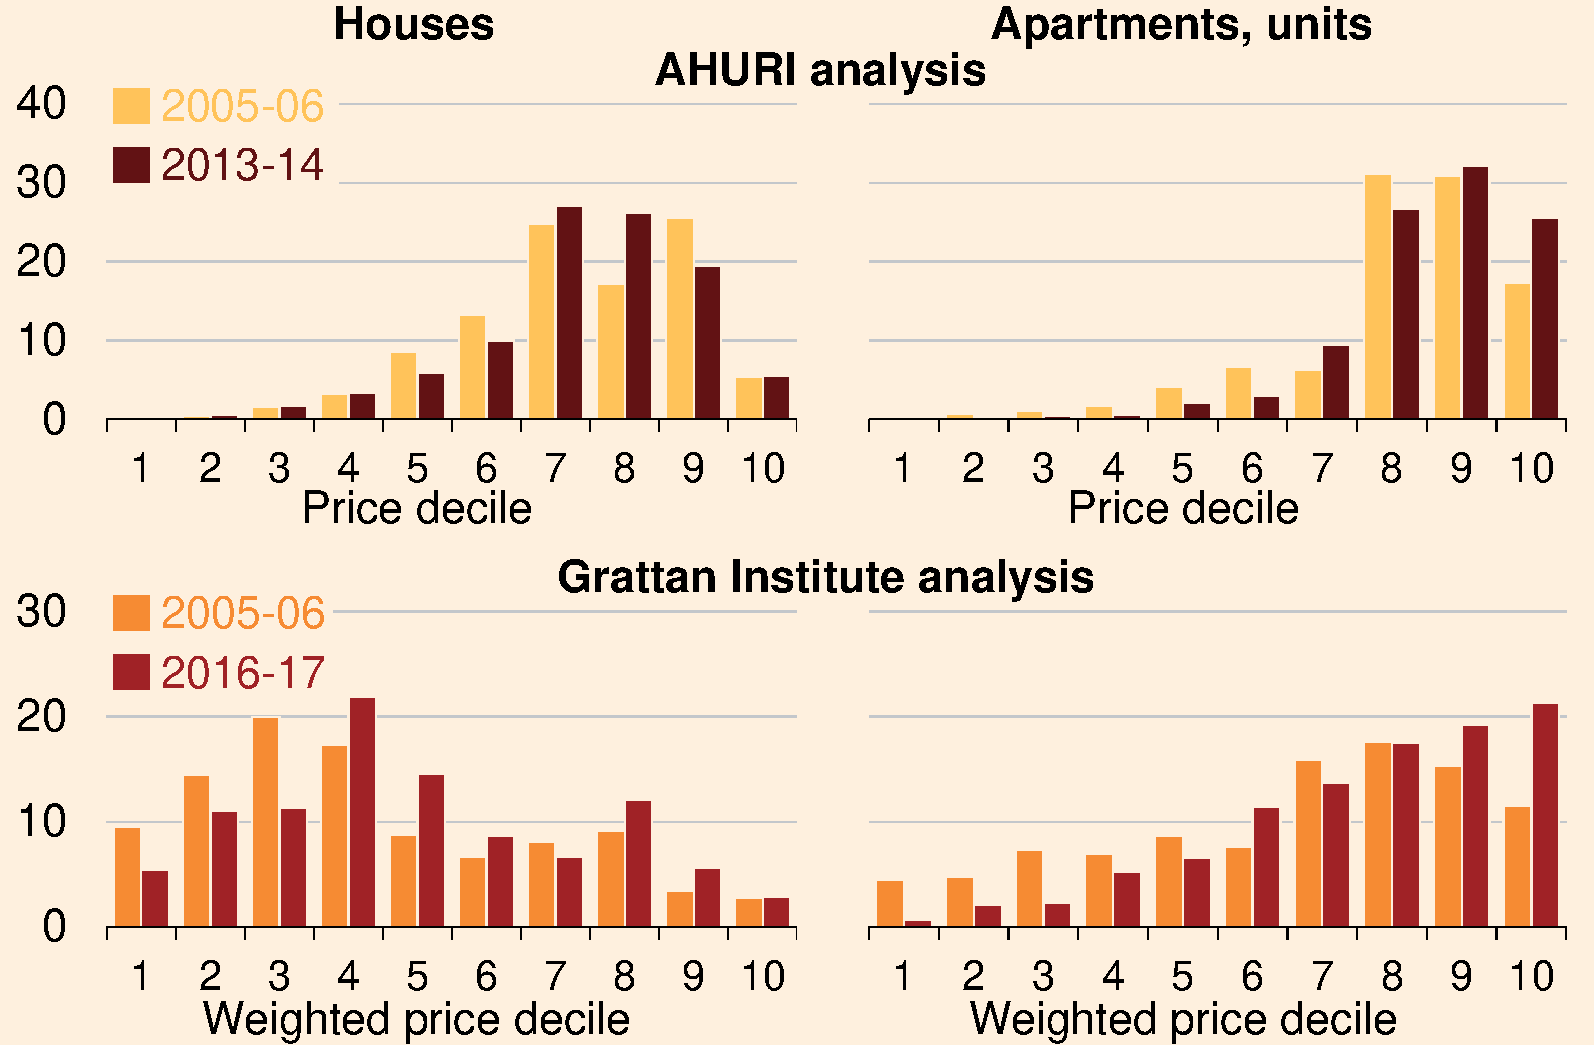
\includegraphics[page=1]{atlas/Approvals_by_weighted_price_decile_long.pdf}
		\noteswithsource{Weighted price deciles are calculated by ranking LGAs according to their median price values, and sorting into deciles weighted by the total dwelling stock in each LGA so that each decile has a similar number of dwellings (LGAs without price data were excluded). All building approvals for an LGA are assigned to the decile that it sits in. LGAs are as they were in 2006 and 2016, with the best available price data assigned to that LGA (some very small LGAs were excluded). `Apartments, units' includes units, apartments, flats, semi-detached, row or terrace houses and townhouses in Grattan analysis. This is consistent with the definition of the CoreLogic price data used to rank LGAs by median house and unit price. In contrast, \textcite{OngEtAl-AHURI-2017-Housing-supply-responsiveness} appear to include semi-detached and townhouses in the `Houses' category.}{\textcites{OngEtAl-AHURI-2017-Housing-supply-responsiveness}{ABS-2017-Building-approvals-Sep-2015}{ABS20016Censuspopulationhousing}{ABS2006}; Grattan analysis based on CoreLogic data.}
		\end{figure}
		
\end{bigbox*}

And even if new housing were biased towards more expensive dwellings, it would still `filter down' to improve affordability for lower-income households.
More housing supply -- even if priced at the top end -- should ultimately free-up less expensive housing stock.
The people who move into newly constructed more expensive housing are either existing residents who move out of less expensive housing, or new residents who would otherwise have added to the demand and pushed up the price of existing housing.
Irrespective of its cost, each additional dwelling adds to total supply, which ultimately affects affordability for all home buyers.%
	\footnote{While gentrification can push up prices in a particular area, the construction of additional housing in total should lead to prices being lower than otherwise overall.}

There is good international evidence to suggest that this `filtering' does occur in practice.
Initially expensive homes gradually become cheaper as they age, and are sold or rented to people with more modest incomes, and this is a strong source of more affordable housing, especially in the private rental market.%
	\footnote{For example, \textcite{Rosenthal2014PrivateMarkets} finds that the US housing stock `filters' by roughly 1.9 per cent a year -- meaning that a 50-year-old home is typically occupied by someone whose income is about 60 per cent lower than that home's first occupant.
	Most of the filtering of once high-end housing to lower-income groups occurs within the first 20 years of a dwelling's life.
	See also \textcite{Taylor2016Perspectives}; \textcite{Somerville-Mayer-2003-govt-reg-affordable-housing}.}
US estimates suggest that 45 per cent of homes that were affordable to very low-income earners in the United States in 2013 had filtered down from owner-occupier or higher rent categories in 1985.%
    \footnote{\textcite{Weicheretal-The-Long-Term-Dynamics-of-Affordable-Rental-Housing}. The authors define affordable housing as rentals that cost no more than 30 per cent of income for households with 50 per cent or less of the median income for the area.}

Of course, if new construction is disproportionately more expensive, then the overall housing stock will become more expensive -- but this ultimately merely reflects choices across the market to spend more on housing in preference to other goods and services.

New expensive housing might not improve the balance between supply and demand if it merely induced additional demand, presumably from overseas purchasers.
But, as discussed above (See \Cref{subsec:tax-settings-encourage-people-to-invest-in-housing}), there is little evidence that overseas purchasers are increasing demand by much more than they increase supply, and even less evidence that they are the \emph{only} purchasers of more expensive housing.

Similarly, filtering may not work effectively if house prices more broadly are rising quickly. For example, \textcite{AHURI-2011-affordable-rental} found that housing was only affordable for 37 per cent of private renters with household incomes in the lowest 40 per cent of the national income distribution in 2006.%
    \footnote{Of course, this hinges on the arbitrary definition of `affordable': the typical household in the bottom 20 per cent of incomes spends 28 per cent of its income on housing (\Vref{fig:spending-on-housing-by-income}). \textcite{AHURI-2011-affordable-rental}
    defined private rental as `affordable' if it cost no more than 30 per cent of the income of households in the bottom two income quintiles.}
New -- or old -- housing is unlikely to become more accessible to low-income earners in a world where overall house prices are rising rapidly, especially if overall housing supply falls behind population growth because of restrictive land use planning rules. This underscores the need for broader reforms to boost housing supply to improve affordability.%
    \footnote{For example, \textcite{Somerville-Mayer-2003-govt-reg-affordable-housing} find that restrictions on the supply of new units lower the supply of affordable units. More demand for higher quality units increases the incentives for landlords to upgrade existing units into a higher quality, higher return housing sub-market.}

While more market housing can make housing more affordable for all Australians, including many low-income earners, some level of subsidies will always be required so that those worst off can afford housing (\Vref{sec:helping-the-bottom}). But making housing cheaper overall will reduce the amount of public subsidy needed to bridge the gap between the market price of housing and what low-income earners can afford to pay.%
    \footcite[][1]{Daley-etal-2017-Submission-Natl-housing-finance}

% TODO: put between page 58 & 59
\clearpage
% \pagestyle{empty}
% 	\pagecolor{OrangeBackground}
	\begin{boxshell}
	\begin{leftfullpage}
	  \begin{mdframed}[style=GrattanFrameBoxA]
	    \captionsetup{labelfont       = {bf, Orange},
		                font            = {bf, Orange},
		                format          = plain,
		                justification   = raggedright,
		                singlelinecheck = false,
		                skip            = 0ex,
		                position        = above}
		  \dummyCaption{The Victorian planning system restricts the supply of new housing and contributes to higher prices\label{box:Victoria-planning-applications}}
		  \captionsetup{format    = plain,
		                font      = {small, bf, theGrey},
		                labelfont = {small, bf, theGrey},
		                position  = above,
		                skip      = 0pt}
		  % Reduced column sep
		  \addtolength{\columnsep}{-23.8pt}%
		  %\pagecolor{OrangeBackground}
		  \begin{multicols}{2}
			  \setlength{\parskip}{4pt plus 1pt minus 1pt}
			  \RaggedRight
				Our analysis of planning approvals in Victoria between 2007 and 2017 shows that the planning approval process is lengthy and costly to developers, and increases prices for home-buyers.%
				  \footnote{\textcite[][402]{Gurran_Phibbs_2013_housing_supply} also find that, `Victoria’s planning system would seem to be far slower and less certain than those of the other jurisdictions'.}
				Dwelling development applications face substantial delays in inner and middle-ring Melbourne council areas, where housing is in greatest demand.
				The typical dwelling application takes over 214 days%
				  \footnote{The median number of days to finalisation for applications that are granted
				  either by council or through VCAT, excluding applications that are not finalised or not granted.
				  Some of the additional time taken may be due to increased complexity of the application, but
				  single dwelling applications, which are typically less complex, also take longer to get approved in most inner-city councils.}
				to get approved in the City of Melbourne, and longer in Port Phillip and Yarra councils (see \Cref{fig:Melb_planning_map}).
				The approvals process is typically much faster in growth area councils.


				Councils where residents are more politically active may be more reluctant to approve development. They have scope to do so in part because the Victorian planning system aims to protect `neighbourhood character,' which is an inherently vague criterion open to differing interpretations.%
				    \footcites{VICDepLWP2017Neighbour}[][64, 72, 91]{Rowley_2017_Vic_planning_system}

				Inner city councils appear to delay development by a similar amount. In addition to the restrictions within their own planning schemes, some councils seem to use different strategies in the application process to delay development. These are reflected by developers tending to use different grounds for applying to VCAT for review in different council areas.
				Port Phillip is more likely to fail to decide within the prescribed time, whereas Glen Eira is more likely to initially reject an application (\Cref{fig:Melb_planning_delays_chart}).

				\begin{figure}[H]
				\caption{Permits take longer for dwelling development applications in inner and middle ring council areas}\label{fig:Melb_planning_map}
				\units{Median days to permit approval for single and multiple dwelling applications by suburb with LGA boundaries, 2007-2017}
				\includegraphics[page=2]{atlas/Melb_planning_delays_map_short.pdf}
				\noteswithsource{Excludes dwellings that do not require a development application. Does not include the time taken if there were multiple applications for the same dwelling}{Grattan analysis of Victorian Planning Permit Activity Reporting System 2017}
				\end{figure}
			\end{multicols}
		\end{mdframed}
	\end{leftfullpage}
	\end{boxshell}
	\begin{boxshell}
	\begin{fullpage}
% 	\pagecolor{OrangeBackground}
	  \begin{mdframed}[style=GrattanFrameBoxB]
	  \captionsetup{labelfont       = {bf, Orange},
	                font            = {bf, Orange},
	                format          = plain,
	                justification   = raggedright,
	                singlelinecheck = false,
	                skip            = 0ex,
	                position        = above}
% 	  \caption*{Box \ref{box:Victoria-planning-applications} (continued): \nameref{box:Victoria-planning-applications}}%
	  \captionsetup{format    = plain,
	                font      = {small, bf, theGrey},
	                labelfont = {small, bf, theGrey},
	                position  = above,
	                skip      = 0pt}
    \addtolength{\columnsep}{-23.8pt}%
	  \begin{multicols}{2}
	  \setlength{\parskip}{4pt plus 1pt minus 1pt}
	  \RaggedRight

		Victoria's planning system is more open to third party reviews than other jurisdictions, and so a higher proportion of planning decisions are reviewed than in NSW.%
		    \textsuperscript{d}

		Development applications in inner city areas are more likely than outer suburban applications to be reviewed by the Victorian Civil and Administrative Tribunal (VCAT). Applications that are reviewed typically take much longer to be finalised.%
			\textsuperscript{e}

		Almost a third of all local council assessed dwelling applications go to VCAT in Melbourne, Port Phillip and Yarra councils. By contrast, less than five per cent go to VCAT in growth area councils (see \Cref{fig:Melb_planning_delays_chart}).%
			\textsuperscript{f}
        These applications are not frivolous: in both Port Phillip and Yarra, the majority ultimately receive development approval.%
        	\textsuperscript{g}

        The delay involved in applying to VCAT increases costs and uncertainty for developers, which are often passed on to purchasers. A slower supply of new dwellings also increases prices (\eg~see \textcite{Mayer_Somerville_2000_land_use_regulation} and \Vref{box:International-supply-literature}).


		\rule{0.2\columnwidth}{0.4pt}\linebreak
		\begin{tabularx}{\columnwidth}{@{}>{\centering\footnotesize}p{1.5em}@{}>{\footnotesize\arraybackslash}X}
		d.~\null &
		    {39 per cent of all Victorian permit applications received were advertised to third parties and 4 per cent were reviewed by VCAT in 2014-15.
		    In NSW, third party objectors must have a `relevant interest' in the development.
		    In 2014-15, less than 1 per cent, of the 106,077 permit applications received were reviewed or appealed (\textcite[][28]{PC-2017-shifting-dial-potential-of-land}).} \\
		e.~\null &
		    {Within inner and middle Melbourne, applications that are approved by council typically take 116 days for single-dwelling applications and 156 for multiple-dwelling applications. But applications that go to VCAT typically take over a year before they are finalised.} \\
		f.~\null &
            {In Port Phillip 83 per cent of applications were granted when taken to VCAT by the developer for failing to decide within the prescribed time.
			In Glen Eira 62 per cent of applications were granted when taken to VCAT by the developer to contest the council’s refusal to grant a permit.} \\
		g.~\null &
            {Of applications to VCAT by developers between 2015 and mid-2017 and decided by mid-2017, the developer succeeded in 86 per cent of cases when they contested some or all of the council's conditions on development, and in 66 per cent of cases when they contested council's outright rejection.
            But developer success at VCAT reflects survivorship bias: most development applications rejected by council are not taken to VCAT.} \\

		\end{tabularx}


		\begin{figure}[H]
		\caption{Dwelling development applications are more likely to go to VCAT in inner and middle ring council areas}\label{fig:Melb_planning_delays_chart}
		\units{Proportion of finalised dwelling applications taken to VCAT 2015-2017}
		\includegraphics[page=2]{atlas/Melb_planning_delays_chart_long.pdf}
		\noteswithsource{Applications to VCAT by objectors are slightly under-represented because when both developer and objectors applied to VCAT, the proposal was classified as a developer application. Only includes applications where the local council was the responsible authority. Excludes applications that had not been finalised by mid-2017 (so the proportion of dwelling applications taken to VCAT between 2007 and 2017 is typically about 5 percentage points higher than shown).}{Grattan analysis of Victorian Planning Permit Activity Reporting System 2017}
		\end{figure}
		\end{multicols}
	  \end{mdframed}
  \end{fullpage}
  \end{boxshell}
\clearpage\nopagecolor
% \pagestyle{scrheadings}



























































































































































































































































































































































































































































































































































































































































































































































































































































































































%!TEX root = ../Report.tex
\chapter{Worsening housing affordability has serious consequences }\label{chap:worsening-housing-affordability-has-serious-consequences}

Australians are spending more of their household budgets on housing than they should. Rising housing costs are eating up a significant share of income growth, especially for low-income earners. Rising housing costs have also contributed to falling home-ownership rates, and this has far-reaching implications for our economy and society. More Australians are missing out on the benefits of owning a home, which include a sense of belonging, a sense of prosperity, the motivation for additional savings, and the basis for investing in a business.

Lower ownership means more people are renting, and for longer.
Given current market structures and government policies, renting is relatively unattractive: it is generally much less secure; many tenants are restrained from making their house into their home; and renters miss out on the tax and welfare benefits of home-ownership.

Rising house prices have contributed to greater inequality.
Home-owners' wealth has increased dramatically due to rising house prices. Younger people and those with lower incomes who have missed out on buying a house are being left behind.
Increasingly, getting the benefits of home-ownership depends on the wealth of your parents.

Higher levels of household debt may also worsen any future economic shock, because people with higher debt are more likely to cut back their spending.

\section{Australians are spending more on housing than they should}\label{sec:Australians-spending-more-on-housing-than-need-to}

The incomes of most Australian households have increased substantially over the past decade.
But when housing costs are considered, low and middle-income households are not doing so well.


\begin{figure}
\caption{Gains to real income have been mitigated by increasing housing expenditure }\label{fig:rising-housing-costs-eating-income-growth}
\units{Change in real equivalised household disposable income including and excluding housing costs growth, 2003-04 to 2015-16, per cent}
\includenextfigure{atlas/Charts-for-housing-affordability-report.pdf}
\noteswithsources{Housing costs include rents for renters and repayments on loans for owners with mortgages.
Growth in income excluding housing costs calculated by subtracting growth in housing costs from growth in disposable income.
Income quintiles are calculated using household disposable income, equivalised by family size.
Bottom two income percentiles are removed. 2003-04 equivalised household disposable income data from \textcite[][Table 1]{ABS-2017-HouseholdIncomeAndWealth-201516}}
{Grattan Institute analysis of \textcites{ABS-HES-201516-Microdata}{ABS-HES-200304-Microdata}; \textcite{ABS-2017-HouseholdIncomeAndWealth-201516}.}
\end{figure}

Rising housing costs matter to everyone.
If land use planning rules and other government policies make housing more expensive, then Australians have less to spend on other goods and services (\Cref{fig:rising-housing-costs-eating-income-growth}).%
    \footnote{For a conceptual discussion of the efficiency costs of land use planning restrictions, see \textcite{GlaeserGyourko2017EconImplications}.}

Incomes for the lowest 20 per cent of households have increased by about 27 per cent since 2003-04.
But with housing costs rising faster than incomes, real incomes \emph{after} housing costs have only grown about 16 per cent over the same period.
Both home-owners and renters in the bottom 20 per cent of income earners are spending more on housing.
Rising housing costs have affected higher income earners less. 


\section{More Australians are missing out on the opportunity to own a home}\label{sec:falling-home-ownership-rates-are-depriving-more-people-of-the-benefits-of-owning-a-home}

Home-ownership rates are falling most dramatically among the young and the poor.
People who cannot buy a dwelling miss out on the economic and social advantages of home-ownership.
Without change, an increasing proportion of Australians born after 1970 will never get on the property ladder.

\subsection{Home-ownership is declining, especially among the young and poor}\label{subsec:home-ownership-is-declining-especially-among-the-young-and-poor}

Home-ownership rose rapidly in Australia in the early 1950s, from around 50 per cent to 70 per cent.%
	\footcite[][2--3]{RBA2015SubmissionHomeOwnershipInquiry}
Home-ownership rose despite rapid population growth, as new homes were built at an unprecedented rate.%
	\footcite[][4]{Eslake-AIST}
Overall home-ownership remained around 70 per cent for the next 50 years, with a slight decline over the past decade to 67 per cent in 2016.%
	\footcite{ABS20016Censuspopulationhousing}
The trends are similar in many other advanced economies.%
	\footcite[][3]{RBA2015SubmissionHomeOwnershipInquiry}

But the ageing of the Australian population has concealed a greater fall in home-ownership rates over the past two decades for all but the oldest households.
Younger Australians have always had lower incomes and less accumulated savings, and hence lower home-ownership rates.
But between 1981 and 2016, home-ownership rates among 25-34 year olds fell from more than 60 per cent to 45 per cent (\Vref{fig:home-ownership-age}).
Only some of this is the result of people starting work, forming long-term partnerships, and having children later in life.%
    \footnote{\textcite{Wood-Ong-2012}.
    There was a small increase in the proportion of 25-34 year olds renting who also owned an investment property between 2003-04 and 2015-16 (sometimes referred to as `rent-vestors': \textcite{Millar2016_rentvestors}).}

\doublecolumnfigure{
\caption{Home-ownership is falling for younger age groups}\label{fig:home-ownership-age}
\units{Home-ownership rate by age, per cent}
\includenextfigure{atlas/Charts-for-housing-affordability-report.pdf}
\noteswithsources{Per cent of occupied private dwellings. Household age group according to age of household reference person. Excludes households with tenure type not stated}%
{\textcites{yates2015submission}{ABS20016Censuspopulationhousing}; Grattan analysis}
}{
\caption{Home-ownership is falling particularly fast for low-income earners}\label{fig:home-ownership-age-income}
\units{Home-ownership rates by age and income, 1981 and 2016}
\includenextfigure{atlas/Charts-for-housing-affordability-report.pdf}
\noteswithsources{Updates \textcite{BurkeStoneRalston2014} using ABS Census special request data.
Household incomes based on Census data are approximate, and so small changes in ownership rates may not be significant.
Excludes households with tenancy not stated (for 2016) and incomes not stated.}%
{Grattan analysis of \textcites{BurkeStoneRalston2014}{ABS20016Censuspopulationhousing}.}
}

Home-ownership has also fallen for middle-age households, suggesting that most of the fall in home-ownership is due to higher dwelling prices rather than changing preferences for home-ownership among the young.%
	\footnote{\textcites{Gradwell2017HousingBalance}{Eslake2013}.
	As shown in \Cref{sec:it-is-getting-harder-to-save-for-a-deposit} and \Vref{sec:the-initial-mortgage-burden-hasnt-changed-much-but-borrowers-are-taking-more-risk-for-longer}, falling interest rates have offset rising prices so that the burden of repaying a new or existing home loan is not particularly high by historic standards.
	But households are taking on more risk for longer, and it is harder to save a deposit.}
Consequently, without intervention, home-ownership rates are unlikely to bounce back over time.
For 35-44 year olds, home-ownership has fallen fast -- from 74 per cent in 1991 to around 62 per cent today -- and home-ownership is also declining for 45-54 year olds.
Current trends are expected to translate into a 10 percentage point fall in home-ownership rates for over-65s by 2046.%
	\footcite{YatesBradbury2010}

The fall in ownership is not the result of changing preferences.%
	\footnote{\textcite[][6]{Simon-Stone-2017-Property-Ladder}, analysing first home buyer behaviour before and after the global financial crisis, found that falling home-ownership rates among younger households are `a reflection of higher housing prices rather than a shift in preferences -- households still have a similar desire to become home-owners, however, fewer potential [first home buyers] are actually able to enter the housing market and purchase a home than before'.} 
Owning a home remains a core aspiration for most Australians. Two-thirds of those aged 25-to-34 responding to a 2017 Australian National University survey thought owning a home was an important `part of the Australian way of life'.%
	\footnote{\textcites{Sheppardetal2017}{Simon-Stone-2017-Property-Ladder}.
	According to this survey, ``Emotional security, stability, belonging' was the main reason people purchase a house, with `investment, financial security'' second.
	Similarly, \textcite[][23]{MissionAustralia2014} found that almost three quarters of 13,600 15-19 year olds considered home-ownership `extremely' or `very' important.}
But more than half of all respondents were `very concerned' that younger generations won't be able to afford a house.

Home-ownership is falling particularly fast for low-income households (\Vref{fig:home-ownership-age-income}).
For 25-34 year olds in the lowest 20 per cent of incomes, home-ownership rates plummeted almost 40 percentage points between 1981 and 2016.



\subsection{People will miss out on the benefits of home-ownership as housing has become less affordable}\label{subsec:people-will-miss-out-on-the-benefits-of-home-ownership-as-housing-has-become-less-affordable}

There are plenty of reasons to care about home-ownership.

For many, home-ownership is a touchstone of progress and prosperity.
Home-ownership has been the norm in Australia since around 1950.%
	\footcite[][7]{KellyHarrisonHunterEtAl2013}
And owning a home can provide a sense of community belonging.%
	\footcite{KellyHarrisonHunterEtAl2013}
In theory, a home can provide many of these benefits whether it is rented or owned.
In practice, home-owners have more permanence, more ability to personalise their home and more control over their surroundings than renters.

Home-ownership is also associated with outcomes such as better health, lower crime, and higher education levels,%
	\footcite{WaldegraveUrbanova2016}
although it is less clear whether this reflects the effects of home-ownership, or the characteristics of the kind of people who can afford to buy a home.

Most recent evidence points to home-ownership improving a person's employment outcomes,%
	\footcites{Munch-etal-2006-Are-homeowners-really-more-unemployed}{WaldegraveUrbanova2016}{Kantoretal2015homeownership}
although some earlier studies find that home-ownership can discourage people from moving to seek better employment opportunities.%
	\footcite{Oswald-1999-Housing-market-and-Europes-unemployment}

Home-ownership is also associated with better financial outcomes.
Home-ownership can provide the motivation to save more, the basis for setting up a business, and collateral for investing. 

Buying a home and taking on a mortgage is one way for households to commit to saving.
Home-owners tend to save more and build more wealth,%
	\footnote{US evidence: \textcites{Dietal2007}{TurnerLuea2009}.}
although it is difficult to determine whether this is because taking on a mortgage imposes savings discipline, or because households with more savings discipline are more likely to buy their home.%
	\footcites{Dietal2007}{TurnerLuea2009}{DietzandHaurin2003}

A family home can be used as collateral to borrow money at lower interest rates than otherwise, making it easier to build other wealth.%
	\footcite[][126]{Connollyetal2015}
Much small business borrowing is backed by security over property.%
	\footnote{\textcite[][126--142]{Connollyetal2015} find some weak evidence of a positive relationship between housing equity and entrepreneurship, but it is hard to disentangle cause and effect. \textcite{CorradinPopov2015}, using US micro-data, find that more home equity increases the likelihood of people becoming self-employed.
	\textcite{Schmalzetal2017} obtain similar results for French entrepreneurship.}

Many people use their own home as security to finance the purchase of an investment property.
Given low interest rates and rapidly escalating prices, leveraging to invest in property has provided high rates of return and increased wealth for those prepared to take the risk over the past few decades.%
	\footcite{CrowleyLi2016}

Home-ownership has been a highway to wealth in part because tax and welfare laws treat it more favourably than other investments (see \Vref{subsec:tax-settings-encourage-people-to-invest-in-housing}).
In 2013, tax and welfare concessions of \$36 billion a year were available for owned homes but not for other investments.%
	\footnote{\textcite[][22--29]{KellyHarrisonHunterEtAl2013}.
	The family home is exempt from capital gains tax and state land taxes, imputed rents are not included in the owner's taxable income, and the pension assets test effectively includes only the first \$200,000 of value of a family home.}
In addition, government subsidies for aged care are less affected if a person owns a home rather than other assets.%
	\footcites{DSS-Exempting-Principal-Home-Care-situations}{OnePath-2013-Aged-care-and-the-former-home} %
Given the substantial private benefits of home-ownership, these tax and welfare concessions for home-owners appear excessive. 	Indeed, home-ownership would remain highly attractive regardless of the level of government support for it.

And home-ownership can have costs. While home-ownership can be a source of personal wealth, it also exposes households to financial risk. Buying a home can require households to put most of their savings and considerable leverage into one potentially volatile asset, reducing their ability to diversify risk.%
    \footcite[][8]{KellyHarrisonHunterEtAl2013}
Meanwhile some research suggests that home-owners' relative lack of mobility can, over time, lead to higher levels of unemployment.%
    \footcite[][8]{KellyHarrisonHunterEtAl2013}
    
Home-ownership matters because that's the system we have. Many aspects of Australian policy have been built on the assumption that most Australians will own their home, including retirement incomes, access to finance, and rental tenure. While many other developed countries, such as Germany, have lower home-ownership, the social outcomes are balanced by different policy settings in many other areas. 

\subsection{Falling home-ownership threatens future retirement incomes }\label{subsec:higher-housing-costs-and-falling-home-ownership-rates-threaten-future-retirement-incomes}

Australia's retirement income system has historically assumed that most retirees would own their home outright.%
	\footcite{Yates2015}
Retirees who have paid off the mortgage are insulated from rising housing costs,%
	\footcites{Yates2015}{Eslake-AIST}
a substantial safety net if they exhaust their retirement savings.
Home-ownership is particularly attractive for retirees because in effect only the first \$203,000 of the value of the home is included in the Age Pension assets test.%
	\footnote{See \Vref{sec:include-the-family-home-in-age-pension-assets-test} for further details.}

\doublecolumnfigure{
\caption{Retirees are more likely to live in private rental housing in future}\label{fig:renters-retirees}
\units{Renters as per cent of population, 2013-14}
\includenextfigure{atlas/Charts-for-housing-affordability-report.pdf}
\sources{\textcites{Yates2016why}{ABS-201314-occupancy-and-costs}}
}{
\caption{Fewer Australians at all ages own their home outright than in the past}\label{fig:outright-owners-age}
\units{Per cent of households that own their home outright, by age group}
\includenextfigure{atlas/Charts-for-housing-affordability-report.pdf}
\noteswithsource{by age of household reference person.
Chart shows data from all available surveys.
Data for 65+ for 2005-06, 2007-08, 2009-10, 2011-12 is estimated using population shares of five-year age groups due to lack of data}%
{\textcites{ABS-SIH-Microdata-200506}{ABS-SIH-Microdata-200708}{ABS-SIH-Microdata-201112}{ABS2015MicrodataIncomehousing}.}
}

But if current trends continue, a greater proportion of people reaching retirement age will be renting -- and more of them will depend on the private rental market rather than social and public housing (\Vref{fig:renters-retirees}).
Among home-owners, more will still be paying off their mortgage when they retire -- the proportion of 55-64 year olds who own their houses outright fell from 72 per cent in 1995-96 to 42 per cent in 2015-16 (\Vref{fig:outright-owners-age}).
Some of these older households will (quite rationally) use some or all of their superannuation savings to pay off their mortgage debt.%
	\footnote{\textcite[][10]{Eslake-AIST}. Of course this undermines the intent of the super system, and means that substantial tax concessions are never used to reduce Age Pension costs.}




\section{Renting is relatively unattractive given current policies }\label{sec:renting-is-relatively-unattractive-under-current-policy-settings}

Home-ownership is popular partly because renting is a relatively poor alternative for many Australians.
As it becomes more difficult to buy a house, more people are renting when they would prefer to own a home.%
	\footnote{In a 2014 survey of 580 renters, 57 per cent of respondents said they rent because they `can't afford to buy' and 10 per cent were `looking to buy' (\textcite{NSW-Tenants-Union-2014-Survey-report}).}
Renting has always been common among young people, but more older people are now renting, with 20 per cent of 45-54 year olds privately renting in 2013-14, up from 12 per cent in 1995-96.%
	\footcites{ABS-SIH-Microdata-200506}{ABS-SIH-Microdata-200708}{ABS-SIH-Microdata-201112}{ABS-HES-201516-Microdata}
Although renting can offer more flexibility, it has many disadvantages: it is often unstable; tenancy laws restrict renters from personalising their homes; and renters miss out on the generous tax and welfare breaks provided to owner-occupiers and property investors.

\subsection{Many renters feel insecure about their housing situation and worry about having to move}\label{subsec:many-renters-have-little-control-over-when-they-have-to-move-house}

Renters have little assurance that they can stay in a place as long as they want.
Most tenancy agreements are for a fixed term of one year (or less).%
	\footcites{Natl-Shelter-2017-Life-in-Aust-private-rental-market}{AHURI-2017-Do-long-leases-long-tenancies}
They often then convert to periodic leases (often referred to as month-by-month leases).

Renters move much more often than owners.
More than 65 per cent of private renters had moved in the past two years, compared to 24 per cent of owners with a mortgage (\Vref{fig:renter-satisfaction-moves}).%
	\footnote{This is consistent with bond repayment data on completed tenancies, which show that in NSW, 66 per cent of tenancies last for two years or less: \textcite{AHURI-2017-Do-long-leases-long-tenancies}.}
\textcite{OngEtAl-AHURI-2017-Housing-supply-responsiveness} found that private renters are approximately 15 percentage points more likely to move than people who own their home outright.%
	\footnote{The authors control for time living at address, house value, area unemployment rate, financial stress and housing costs: \textcite[][50]{OngEtAl-AHURI-2017-Housing-supply-responsiveness}.} 

\begin{figure}
\caption{Renters move more often than owners and are less happy with their lot}\label{fig:renter-satisfaction-moves}
\includenextfigure{atlas/Charts-for-housing-affordability-report.pdf}
\sources{\textcite{ABS-201314-occupancy-and-costs}; Grattan analysis}
\end{figure}

Many of these renters were forced to move.%
	\footnote{\textcites{ABS-201314-occupancy-and-costs}{KellyHarrisonHunterEtAl2013}{Ellis-2017-Speech-Aust-Housing-Researchers}.
	The difference in mobility between owners and renters in Australia is the highest in the OECD (\textcite{KellyWeidmannWalsh2011}).
	A 2014 survey of NSW renters found that 14 per cent who had moved in the past three years were evicted by their landlord (\textcite{NSW-Tenants-Union-2014-Survey-report}).}
Being forced to move, or worrying about the possibility of having to move, is a particular problem for families with children in school, for those who are psychologically distressed by the change (often older people), and for those who struggle to afford the costs of moving (often poor people).%
	\footnote{Some 92 per cent of respondents to the 2014 survey of NSW renters said they were worried about moving due to concerns about finding a suitable house at a rent they can afford (\textcite{NSW-Tenants-Union-2014-Survey-report}).}

Insecurity of tenure for renters is increased by three factors: state land tax regimes that generate short-term leases; tax incentives that encourage landlords to turn properties over more often to maximise negative-gearing benefits; and standard lease terms and tenancy laws that provide landlords with broad rights to terminate leases unilaterally.%
	\footcite[][26]{DaleyWood2016-Negative-Gearing-CGT}
	
Tenants may also be reluctant to commit to a long lease.
Under current laws, long-term leases create significant financial risk for tenants if their circumstances change and they need to move, because tenants are liable to pay rent until the end of the fixed-term lease, or until a new tenant is found.%
	\footnote{\textcite{James-2015-Should-Aust-adopt-10yr-leases}. To encourage longer leases, the Victorian Government is introducing new standard long-term leases (\textcite{VicStateGov2017Homes}).}

\subsubsection{State government land taxes make short-term leases common and contribute to insecurity of tenure }\label{subsec:state-government-land-taxes-make-short-term-leases-common-and-contribute-to-insecurity-of-tenure}

Tenancy laws allow longer leases, but few landlords agree to them.%
	\footnote{About 94 per cent of fixed-term private rental agreements have a lease lasting 12 months or less (\textcite{Hulse-etal-2011-AHURI-Secure-occupancy-rental-housing}).}
Short leases are in part a result of state government land taxes that lead to most residential investment properties being owned by small, `mum and dad' landlords.\footcite{AHURI_2018_private_rental_housing_Martin_etal}
According to 2014-15 taxation statistics, 86 per cent of rental properties are owned by landlords with three properties or fewer (\Vref{fig:rental-owenrship-numbers}).%
	\footnote{Institutional investors make up a much larger share of landlords in the US and Germany (\textcites{Shaw-2014-theConvo-Renting-for-life}{Chong-2016-theOz-MacqGrey-align-rental-home-market}).}

\begin{figure}
\caption{Less than 15 per cent of residential investment properties are owned by landlords with more than three properties}\label{fig:rental-owenrship-numbers}
\units{Share of total investment properties by number of properties owned by investor, 2014-15}
\includenextfigure{atlas/Charts-for-housing-affordability-report.pdf}
\noteswithsources{An interest in a property means the property is either solely owned, or jointly owned for all or part of the year.
Excludes those that own no residential property other than their primary residence}%
{\textcite{ATO-2017-Landlords-2006-to-2014}; Grattan analysis}
\end{figure}



State government land taxes disadvantage institutional investors relative to `mum and dad' landlords who own only one or two properties.%
	\footcites[][Volume~1, pp.~261--262]{HenryTaxReview2010}[][15]{DaleyCoates-2015-Property-taxes}[][14]{mclaren2014uniform}[][69]{Hulse-etal-2011-AHURI-Secure-occupancy-rental-housing}
State land taxes, with generous tax-free thresholds and progressively higher taxes based on a person's total land holdings by value, lead to large landowners paying much higher rates of land tax on a given investment property than if that same property were owned by a small investor (\Vref{fig:land-tax-investors}).%
    \footnote{Institutional investors do tend to own commercial properties as each property tends to be more valuable, and therefore attracts a higher land tax rate.
    Consequently, for most commercial properties small-scale investors have much less of a tax advantage. However, small commercial properties, such as post offices, still tend to be owned by small investors (\textcite{Prosper_2014_Freebairn_speech_press_release}).}
Even a landlord with three properties may be paying minimal land tax if each property is in a different state, because land tax thresholds are based on the aggregate landholdings in any one state.
But a large landholder would pay land tax of around 2 per cent of the land value (typically 1 per cent of the property value including improvements),%
	\footcite{DaleyCoates-2015-Property-taxes}
whereas an individual investor with only one rental property might well pay no land tax at all on the same property.%
	\footnote{The top land tax rate is typically levied on landholdings over about \$2 million. The top rate is 2.0\% in NSW, 2.225\% in Victoria, 1.75\% in Queensland, 2.67\% in Western Australia, 3.7\% in South Australia, and 1.5\% in Tasmania.}


\begin{figure}
\caption{Progressive land taxes discourage large investors from holding residential property}\label{fig:land-tax-investors}
\units{Annual land tax paid and post-tax income return, per cent of asset value}
\includenextfigure{atlas/Charts-for-housing-affordability-report.pdf}
\noteswithsources{Assumes a small investor owns one property, a medium investor owns five properties and a large investor owns 25 properties. Sydney example based on \$880,000 median-priced dwelling. Melbourne example based on \$720,000 median-priced Melbourne dwelling. Brisbane example based on \$490,000 median-priced Brisbane dwelling and `large investor' is subject to land tax regime for resident individuals. For all three cities, assumes 4 per cent gross rental return and land value is assumed to be half the value of the property.  Ignores deductibility of land tax costs against income in personal and corporate income tax returns}{\textcites{NSW_rev_office_2018_land_tax}{Vic-SRO-2017-Land-tax-current-historical-rates}{StateRevenueQueensland2018_land_tax}{ABS-2017-Residential}; Grattan analysis}
\end{figure}

The difference is material.
For example, a small investor might own and rent out one median-priced Sydney home worth \$880,000, and would pay no land tax (assuming \$440,000 land value).
By comparison, a large investor owning 25 such properties would pay \$7,915 in land tax on each property.%
	\footnote{Based on NSW land tax rates for the 2016-17 financial year.}
Assuming a net rental yield of 4 per cent, the large investor loses roughly one quarter of the rental return in land tax (\Vref{fig:land-tax-investors}).
If individual and institutional investors have similar target rates of return, the individual investor would be prepared to pay about 30 per cent more for a given investment property.\footnote{Institutional investors face less of a disadvantage for high density housing, such as apartments or student accommodation, since the land share of the dwelling cost is lower due to higher construction costs for taller buildings.}

As a result, small investors dominate Australia's rental housing market.
Mum and dad investors are reluctant to offer long-term leases, or otherwise guarantee more secure tenure to tenants, because they wish to maintain control over an asset that accounts for a large share of their overall wealth holdings, and which they may need to liquidate quickly.%
	\footnote{\textcite{Wood-Ong-AHURI-2010-factors-affecting-landlords} found that one in four residential property investors exit the market each year.}

\subsubsection{Negative gearing results in shorter lease terms }\label{subsec:negative-gearing-results-in-shorter-lease-terms}

Negatively geared landlords are particularly likely to turn over properties regularly, and are less likely to care about satisfying tenants' needs.%
	\footcite[][26]{DaleyWood2016-Negative-Gearing-CGT}
By contrast, institutional investors in multiple properties who want liquidity will usually have at least one vacant property to sell, even if they provide long-term leases, because of the inevitable turnover of individual tenants.

\subsubsection{Landlords' rights to terminate a lease compound renter insecurity }\label{subsec:landlords-right-to-terminate-a-lease-without-grounds-compounds-renter-insecurity}

Tenancy laws are supposed to ameliorate some of the unequal bargaining power that landlords often have over tenants.
But landlords often have the upper hand in negotiations if the tenant needs to get a roof over their head quickly -- the consequences of being homeless for a week are much greater than missing out on one week's rent.
Some argue that current laws are tilted too far in favour of landlords.%
	\footcites{Power-2017-theConvo-For-renters-housing-affordable-just-the-start}[][8]{Natl-Shelter-2017-Life-in-Aust-private-rental-market}{Irvine-2016-SMH-Hidden-tax-hurts-renters}

One of the most contentious parts of state tenancy laws is allowing landlords to evict tenants `without grounds', albeit with a notice period.
For example, in Queensland, a landlord can evict a tenant without grounds with two months' notice.%
	\footnote{\textit{Residential Tenancies and Rooming Accommodation Act 2008} (Qld) s.291, s.329(2)(k)(i).
	The period of notice varies.
	In Victoria, the notice period is 90 days at the end of a fixed-term lease, and 120 days for a periodic lease (\textcite{Consumer-Affairs-Vic-Landlord-giving-notice-to-vacate}).
	In NSW, the notice period is 30 days at the end of a fixed-term lease and 90 days for a periodic lease (\textcite{NSW-Fair-Trading-Giving-termination-notice}).
	In the ACT, the notice period is 26 weeks (\textcite{Morris-etal-2017-theConvo-Insecurity-private-renters}).}
Tenancy advocates and some commentators argue that without-grounds evictions are the major contributor to renter insecurity.%
	\footcites[][66]{Hulse-etal-2011-AHURI-Secure-occupancy-rental-housing}{Power-2017-theConvo-For-renters-housing-affordable-just-the-start}[][8]{Natl-Shelter-2017-Life-in-Aust-private-rental-market}{Irvine-2016-SMH-Hidden-tax-hurts-renters}[][12--13]{Adkins-etal-2002-Tenure-security-Qld}{Martin2017renting}
Although only a small share of tenants are evicted without grounds -- a recent survey found 17 per cent of renters had been evicted without grounds or with no reason given -- the possibility creates insecurity and stress.%
	\footnote{\textcite{Morris-etal-2017-theConvo-Insecurity-private-renters} `for at least one in four of our interviewees, the chronic de jure insecurity associated with private renting imbued everyday life with ongoing anxiety and stress'.
	According to \textcite{NSW-Tenants-Union-2014-Survey-report}, 92 per cent of respondents are worried about moving.}
Without-grounds evictions can also deter tenants from exercising their rights, such as requesting legitimate repairs or contesting a rent increase.%
	\footnote{According to \textcite{Natl-Shelter-2017-Life-in-Aust-private-rental-market}, of people who had a problem with their rental property but didn't complain, 37 per cent feared eviction or not having their lease renewed.
	\textcite[][12]{Adkins-etal-2002-Tenure-security-Qld} found that people are worried about contesting rent increases due to fear of retaliatory `without grounds' eviction.}

In many states, landlords can terminate a lease with even less notice for a variety of reasons, including that the landlord decides to sell the property or live in it themselves.%
	\footnote{See for example \emph{Residential Tenancies Act 1997} (Vic) ss 258-259.}

\subsection{Renters are less satisfied with their home, and laws restrict renters from making the place they rent feel like their `home'}\label{subsec:renters-are-less-satisfied-with-their-home-and-laws-restrict-renters-from-making-the-place-they-rent-feel-like-their-home}

Renters are generally less satisfied than owners with their home, although this partly reflects how the average renter has a lower income and so lives in lower quality housing. (\Vref{fig:renter-satisfaction-moves}).%
	\footcite{ABS-201314-occupancy-and-costs}
Renters are more likely to live in a house with a major structural problem.%
	\footnote{In 2013-14, 18 per cent of private renters were living in a dwelling with a major structural problem, compared to 11 per cent of owners and 32 per cent of public renters \textcite{ABS-201314-occupancy-and-costs}.}
Some renters report fearing eviction or a rent increase if they request legitimate repairs or maintenance.%
	\footnote{Retaliatory evictions are illegal, but it is difficult for tenants to prove the landlord's motive was retaliation.}

Tenancy agreements typically restrict renters from making the place they rent feel like their `home'.%
	\footcite{KellyHarrisonHunterEtAl2013}
Tenants usually need their landlord's consent to make even small alterations, such as putting picture hooks in walls or changing the garden.
And even if tenants can make improvements, usually they lose them if they move.
Tenants usually need their landlord's consent to keep a pet, even if the property is suitable and a bond is paid.%
    \footnote{If the value of a pet to a tenant is greater than the cost to the landlord, then in a perfect world, tenants and landlords would contract to allow a pet in return for slightly higher rent (\textcite{Coase_1960_social_cost}).
    But in practice, the allocation of rights under standard contracts and legislative defaults tends to determine outcomes because they anchor expectations, and because transaction costs are material.}
Prospective tenants with pets also report feeling discriminated against when applying for a property.%
	\footcites{Natl-Shelter-2017-Life-in-Aust-private-rental-market}{Sparvell-2016-Vic-renters-may-soon-have-pets}

\subsection{Renters miss out on tax advantages available to home-owners and property investors}\label{subsec:renters-miss-out-on-tax-advantages-available-to-home-owners-and-property-investors}

Renters miss out on the significant tax and welfare incentives for home-owners and property investors, as described in \Vref{subsec:tax-settings-encourage-people-to-invest-in-housing} and \Vref{subsec:people-will-miss-out-on-the-benefits-of-home-ownership-as-housing-has-become-less-affordable}.
While renters may benefit a little from tax breaks for property investors, when land supply is constrained due to land use planning rules, tax breaks for property investors are mostly capitalised into house prices rather than passed on as lower rents.
Some renters benefit from Commonwealth Rent Assistance, but this is less than 6 per cent of the total housing benefits that governments provide.%
	\footnote{\textcite[][22--29]{KellyHarrisonHunterEtAl2013}. Commonwealth and state governments also spend around \$5~billion each year on social housing.
	Although social housing is outside the scope of the report, government additions to public rental stock are likely to benefit renters in the private rental sector by reducing rental demand.}
By contrast, home-owners and investors receive more than 90 per cent of the benefits of major housing policies.
And some of the burden of land tax is probably borne by tenants via higher rents, because owner-occupied properties are land-tax exempt.%
	\footcite[][210]{HenryTaxReview2010}
Partly as a result of these tax and welfare policies, buying was financially more favourable than renting an equivalent house for most of the past three decades in major Australian cities.%
	\footcite{CrowleyLi2016}
	
Many people are renters, particularly the young and poor, by necessity not choice (\Vref{fig:home-ownership-age-income}). Because low-income earners are now much less likely to be home-owners, tax breaks favouring home-ownership increase inequality, especially as these tax breaks become more valuable when house prices rise.

\section{Higher housing prices mean people struggle to live near where most jobs are being created}\label{sec:higher-housing-costs-mean-people-struggle-to-live-near-where-most-jobs-are-being-created}

A generation ago, more jobs, particularly in manufacturing, were dispersed among the suburbs.%
	\footcite{KellyDonegan2015-City-limits}
Now, more new jobs are located in and around CBDs.
With agglomeration, average incomes rise.%
	\footnote{See above \vpageref{paragraph:cities-increase-incomes}.}
But as jobs growth is becoming more concentrated, younger generations that can only afford to buy the newly built housing on the city fringe are living further from the city centre than their parents did when they bought their first homes.
Instead of enduring longer commutes, many young people are instead renting for longer.

New and less expensive housing has always been built on the edge of our cities.
But the urban fringe is much further away from the centre than 30 years ago.
In Melbourne, suburbs around 20km from the CBD, such as Glen Waverley, Altona and Bundoora, were new suburbs in 1970s; today the city fringe can be more than 50km from the CBD in the south-east.%
	\footcite[][Map~1]{VicGovPlanMelb2017}
In Sydney, new developments in the south-west can be more than 60km from the CBD.%
	\footcites[][Figure~2]{NSW-DPE-2014-Plan-for-growing-Syd}{Transport-Sydney-2014-Sydneys-urban-growth-history}
And whereas 30 years ago first home buyers in large capitals had the option of some relatively cheap housing in inner-ring suburbs such as Surry Hills in Sydney, Richmond in Melbourne and New Farm in Brisbane, most of these suburbs have gentrified and are typically beyond the reach of first home buyers.%
	\footcites{coffee-visualising-pop-change}[][19--20]{KellyMaresHarrisonEtAl2013}

The increasing distance between where jobs are located and where new housing is built has personal and broader economic costs.%
	\footnote{\textcites{KellyDonegan2015-City-limits}{NBER2017HsiehMoretti}{Cheshireetal_2018_empty_homes}.} 
The costs of this divide include fewer job opportunities, heavier traffic congestion, longer commute times and a big drop for many people in the quality of their family and social life.%
	\footcites{KellyDonegan2015-City-limits}{Ryan-Selim-2017-theConvo-Liveable-Sydney-has-clear-winners-and-losers}[][1]{Pawson-et-al-2015-Addressing}{IA_2018_Future_cities}
Long commutes mean it is harder for both parents to work, with women generally the ones who end up working less than otherwise.%	
	\footcite{Daley-2015-Guardian-Inner-city-v-outer-suburbs-where-you-live-really-does-determine-what-you-get}
Female workforce participation in outer suburban areas is typically 20 percentage points lower than for men.%
	\footcite{KellyMaresHarrisonEtAl2013}

These factors also lead to cities stratifying between lower-income households on the fringe and more prosperous households in inner and middle suburbs (see \Vref{subsec:higher-house-prices-are-contributing-to-a-greater-divide-between-the-have-and-have-nots-in-our-cities}).

\section{Higher housing costs have economic costs}\label{sec:higher-housing-costs-have-economic-costs}

Building more new homes in desirable areas near high-paying jobs -- usually towards the centres of capital cities -- doesn't just keep a lid on prices; it can also help the economy.
Research in the US shows that development restrictions limiting housing near high-paying, productive jobs can significantly reduce economic growth.%
    \footcites{GlaeserGyourko2017EconImplications}{NBER2017HsiehMoretti}{Parkhomenko2016}{Herkenhoff2017EmpireStates}{AndrewsEtAlHousing}
Higher housing costs dissuade people from moving to cities where higher-paying jobs are located.
Recent US studies estimate that GDP would be between 2 and 13 per cent higher if enough housing had been built in cities with strong jobs growth such as New York and San Francisco.%
    \footnote{\textcites[][22--24]{GlaeserGyourko2017EconImplications}{NBER2017HsiehMoretti}.
    While the precise estimates of the GDP impact are highly sensitive to assumptions about elasticities of labour demand and the degree of labour mobility, even under conservative assumptions the GDP impact of increasing housing supply in high-productivity cities is large.}

Even when there is no movement between cities, higher housing costs impose economic costs. If people are forced to live on the edge of cities with less access to jobs, then employers have a smaller pool of workers to choose from, and so productivity is lower than otherwise.%
	\footcite[][1]{Pawson-et-al-2015-Addressing}


\section{Rising house prices are widening inequality between generations}\label{sec:rising-house-prices-have-widened-inequality-both-across-and-within-generations}

Rising dwelling prices and falling home-ownership rates are increasing wealth divides between generations.
Older people have benefited from the large increase in house prices over the past 30 years as interest rates fell.
This is a once-off change that is unlikely to recur to help younger generations.
Higher housing costs are forcing younger generations to stay at home for longer.
And the widening inequality \emph{between} generations is beginning to increase inequality \emph{within} generations as more young people are relying on wealthy parents to enter the housing market


\subsection{Rising house prices increase the risks that younger generations will be worse off than their parents}\label{subsec:rising-house-prices-increase-the-risks-that-younger-generations-will-be-worse-off-than-their-parents}

Our 2014 report for Grattan Institute, \citetitle{DaleyWoodWeidmannHarrison-2014-Wealth-of-generations}, showed that today's generation of young Australians are at increasing risk of being worse off than their parents.%
	\footcite{DaleyWoodWeidmannHarrison-2014-Wealth-of-generations}
Older Australians are capturing an increasing share of the nation's resources.
Despite the global financial crisis, 65-74 year old households today are \$480,000 wealthier in real terms than households of that age twelve years ago (\Vref{fig:net-wealth-age}).
Households that were 35-44 years old in 2005-06 increased their average wealth by almost \$600,000 in the following decade.
\oneraggedpage
    
\begin{figure}
\caption{The wealth of older households has increased in ways that are unlikely to be repeated}\label{fig:net-wealth-age}
\units{Mean wealth per household, \$2015-16, thousands}
\includenextfigure{atlas/Charts-for-housing-affordability-report.pdf}
\source{\textcite{ABS-HES-2015-16-Summary}}
\end{figure}

In part, the wealth of generations diverged because of the boom in housing prices (\Vref{box:who-wins-and-loses}).
Older households that owned homes at the start of the house price boom made big capital gains.%
    \footnote{For households headed by 65-74-year-olds and 55-64-year-olds, property contributed about half of the total increase in wealth between 2003-04 and 2015-16 (\textcite{WoodWiltshire2017WoG}).}
These households enjoyed a significant, untaxed windfall gain from rising prices and they continue to benefit from house prices remaining high.
Households that did not own property before the boom -- disproportionately the younger generation -- missed out on the windfall boost in wealth from the price rises.
25-34 year old households today are no more wealthy than the equivalent households a decade before (\Vref{fig:net-wealth-age}).%

The windfall rise in prices is unlikely to be repeated, even if the fundamentals of the real estate market keep house prices high.
Many observers believe that prices are unlikely to grow in future as quickly as they did over the past two decades, because income growth is likely to be slower, and official interest rates can't fall much further.%
	\footnote{\textcites{Eslake-why-housing-expensive}{FoxTulip2014overvalued}{CoreLogic2017}[][31]{DaleyWoodWeidmannHarrison-2014-Wealth-of-generations}.
	At the time of writing, the cash rate, the interest rate set by the Reserve Bank of Australia, was 1.5 per cent.}
As a result, young people are likely to face higher housing costs for a long time.
By contrast, older people who have benefited from the boom may face higher housing costs for only a few years, and can spend housing wealth on other things by downsizing or withdrawing equity.


\begin{smallbox}{Who wins and loses from higher house prices}{box:who-wins-and-loses}
Rising house prices are a mixed blessing. They make existing home-owners and investors feel wealthier. But they are usually bad news for those who don't own a home already. The difference reflects how spending on housing has a dual role.
An owner-occupied home is \emph{both} a place to live and \emph{also} a valuable asset.%
	\footcite{Freebairn2016Housing} 

Housing is unlike most goods and services, which don't provide a financial return.%
	\footcite{FlavinYamashita2002Housing}
And housing is unlike most investments, which are not usually consumed by their owner.
Most people care more about the value of their home as a place to live than as an investment.%
	\footcite{IoannidesRosenthal1994Housing}

So whether a person wins or loses from rising house prices depends on their circumstances.%
    \footnote{Hence \textcite{Lowe2017Householddebt} described rising house prices as a `two-edged sword'.}
Investment property owners are clear winners.
Older home-owners are likely to win if they later downsize.
Younger home-owners benefit even less – their home is worth more, but they still need somewhere to live – and they can be worse off if it costs them more to upgrade to a better home in future.
Renters are worse off if house prices rise because they reflect expectations of higher housing costs in future.%
	\footcite{Lowe-national-balance-sheet-speech}

Consequently, rising house prices affect generations differently: they tend to benefit the older at the expense of the young. 

If house prices do rise even further in future, it may benefit younger generations who meanwhile buy a house. But it will also increase housing costs for the following generation even more. 

\end{smallbox}


Housing inequality between generations contributes to young people leaving home later.
Worsening housing affordability is likely a major cause of the stall in the long downward trend in average household size.%
	\footnote{\textcites{Eslake2013}[][24]{McDonaldTemple-2013-Projs-Housing-demand-Aust}; \Vref{subsec:undersupply-led-to-larger-households}.}
Although sources differ on the scale of the change, young people are leaving home later. 
Census data shows a small increase in the proportion of people in their 20s and 30s living with their parents, particularly in Melbourne and Sydney, and fewer young people living alone.%
    \footnote{For example, the proportion of 25-29 year olds in Sydney living with parents or grandparents increased from 19.7 per cent in 2006 to 21.3 per cent in 2016.}
But the HILDA survey suggests the shift may be larger: it estimates that the proportion of women aged 22-25 living with their parents increased from 27 per cent to 48 per cent between 2002 and 2015, and the proportion of 22-25 year old men living with their parents increased from 43 per cent to 60 per cent.%
	\footcite[][Figure~2.1]{Wilkins2017-HILDA-Selected-findings}
And the share of younger Australians aged 20-34 that are starting their own households has fallen sharply since 2001. The share that do start a household is lowest in Sydney and Melbourne where house prices are highest (\Vref{fig:headsip-ratio}).


\begin{figure}
\caption{Younger Australians are adapting to rising housing costs by starting new households much later in life}\label{fig:headsip-ratio}
\units{Proportion of 20-34 year olds that are the head of their household, per cent}
\includenextfigure{atlas/Charts-for-housing-affordability-report.pdf}
\noteswithsources{Includes both home-owners and renters. In fact a lot of younger people are renters even when they do move out.}
{\textcite{Gradwell2017HousingBalance}}
\end{figure}

 


There is also a growing number of group households and multi-family households.%
	\footnote{According to the Census, between 2006 and 2016 the proportion of 25-29 year olds living in group households increased from 10 per cent to 13 per cent in Sydney and Melbourne respectively. Using HILDA data, \textcite[][6]{Wilkins2017-HILDA-Selected-findings} found that the proportion of `multiple family' households increased from 2.5 per cent to 4 per cent between 2001 and 2015. In the United Kingdom, younger renters have less space per person in a household than 20 years ago, whereas all owners have more space per person (\textcite{Corlett-Judge-2017-Housing-across-gens}).}
Particularly in Sydney, people have built many more `granny flats', which often house family members.%
	\footcites[][21]{Thomas-2016-Housing-supply-outcomes-from-Sydney-codification}{FuaryWagner-2015-Domain-Sydney-in-midst-of-grannyflat-boom}

\subsection{Intergenerational inequality contributes to intra-generational inequality}\label{subsec:rising-house-prices-will-also-contribute-to-intra-generational-inequality-over-time}

The increasing divide between generations can easily become an increasing divide within generations.

For many younger people, the only way they can afford to buy a house is with family assistance.
Indeed, as house prices have increased, more first home buyers are receiving assistance from family and friends to buy a house (\Vref{fig:assistance-to-buy-house}).%
	\footnote{\textcite{Ellis-2017-Speech-Aust-Housing-Researchers}.
	According to National Australia Bank data, 8 per cent of first home buyers taking out a loan in 2015 had a family member acting as a guarantor,
	 an increase from 6.7 per cent in 2015 and 4.8 per cent in 2010 (\textcite{Yeates-2016-more-parents-guaranteeing-kids}).}
If home-ownership relies more on the `bank of mum and dad', then getting a home depends more on the success of one's parents than on one's own endeavours.%
	\footnote{\textcite[][6--7]{RBA2014SubmissionAffordableHousingInquiry}.
This is also occurring overseas: \textcite{Gholipour-etal-2016-theConvo-Higher-property-prices-linked-to-ineq}.}

\begin{figure}
\caption{More first home buyers are receiving assistance from family and friends}\label{fig:assistance-to-buy-house}
\units{Share of all first home buyers receiving assistance from family or friends}
\includenextfigure{atlas/Charts-for-housing-affordability-report.pdf}
\source{\textcite{Ellis-2017-Speech-Aust-Housing-Researchers}.}
\end{figure}

Patterns of inheritance mean that more intergenerational inequality tends to lead to more inequality within generations. 
Large inheritances and bequests have not been common in Australia to date.%
  \footnote{Of the estimated 13 per cent of people receiving an inheritance between 2002 and 2012, more than three quarters received less than \$100,000 and most less than \$50,000 (\textcite[][37]{DaleyWoodWeidmannHarrison-2014-Wealth-of-generations}).} 
But the strong growth in the wealth of today's older generations, combined with the steady shrinking of the family size from 1960 to 2000, may lead to more and larger inheritances and greater inequality.

Bequests are likely to be larger in future. Older households are much richer today than in the past.
And most older households -- particularly wealthier households -- largely maintain (and many increase) their wealth in retirement.
According to one Australian study, the median pensioner dies with residual wealth equal to 90 per cent of the assets recorded at the start of its eight-year investigation.%
	\footcite[][4]{WuEtAlAgePensioner2015}

Inheritances tend to transmit wealth to children who are already well-off.%
	\footcite{DaleyWoodWeidmannHarrison-2014-Wealth-of-generations}
Those who receive an inheritance, and who receive a larger inheritance, are more likely to own their own home already.%
	\footcite{Barrett-etal-2015-Intergen-xfer-housing-econ-outcomes}

This has been the pattern for a long time internationally, and for at least the past decade in Australia (where data on inheritance is relatively scarce).
If the patterns continue, then wealth will ultimately be much less equally shared within younger generations.


\section{Rising housing costs are widening inequality within generations}\label{sec:rising-house-prices-have-widened-inequality-within-generations}

Rising housing costs have bitten much more into the incomes of households at the bottom.
Rising housing prices have increased wealth inequality.
And high house prices have also widened the geographic divide between high- and low-income earners, which tends to translate into even less equal social outcomes.


\subsection{Higher housing costs are hurting those with lower incomes the most}\label{subsec:higher-house-prices-hurting-bottom}

Higher house costs are hurting low-income households the most.
The bottom 20 per cent of households are spending more of their income on housing (\Vref{fig:spending-on-housing-by-income});
cheaper housing has increased in price by more than more expensive housing (\Vref{fig:house-price-deciles});
lower-income renters in capital cities are under increasing financial stress (\Vref{fig:rental-stress-by-area});  
the public housing stock has not kept up with population growth (\Vref{fig:public-housing-stock}); 
and home-ownership rates have fallen the most among those on low incomes (\Vref{fig:home-ownership-age-income}).


\subsection{Rising house prices are increasing wealth inequality }\label{subsec:rising-house-prices-increased-wealthinequality}

Rising house prices have contributed to widening wealth inequality.
Over the past 12 years, the wealth of the richest 20 per cent of households increased by over 50 per cent in real terms, whereas the wealth of the bottom 20 per cent increased by only 10 per cent (\Vref{fig:wealth-income-real-growth}).

Over the same period, income growth was much more even, although the gap between high and low income earners was larger after taking housing costs into account (\Vref{fig:rising-housing-costs-eating-income-growth}). 

\begin{figure}
\caption{Incomes have risen across the board but wealth has concentrated among the rich}\label{fig:wealth-income-real-growth}
\units{Real growth from 2003-04 to 2015-16 per equivalised household quintile}
\includenextfigure{atlas/Charts-for-housing-affordability-report.pdf}
    \noteswithsource{Income estimates for 2003–04 onwards are not perfectly comparable with estimates for 2015-16 due to improvements in measuring income introduced in the 2007–08 cycle. Bottom two income percentiles are removed in disposable income panel. Disposable income numbers differ slightly to \Cref{fig:rising-housing-costs-eating-income-growth} due to differences between ABS and Grattan Institute calculations of income quintiles.}
{\textcite{ABS-2017-HouseholdIncomeAndWealth-201516}}
\end{figure}


\subsection{The geographic divide of our cities is widening the gap between haves and have-nots}\label{subsec:higher-house-prices-are-contributing-to-a-greater-divide-between-the-have-and-have-nots-in-our-cities}

There have always been poorer and wealthier areas within our cities, but this geographic inequality is growing, with rising house prices a contributing factor.
Incomes increasingly determine where you live.
And location increasingly influences a range of social outcomes.

As house prices rise, how much you earn and how wealthy your parents are will increasingly influence where you live.%
	\footnote{\textcite[][182--183]{Rethinking-the-economics-of-land-and-housing-2017}.
	\textcite{Ganong-Shoag-2017-Why-has-regional-income-convergence-declined} argue that reduced mobility resulting from constrained housing supply exacerbates inequality, because when low-income workers move to a state with restricted housing supply, the increases in housing costs can outweigh the potential gains in income.}
Rapidly rising house prices in established suburbs have pushed many people with lower incomes further away from city centres.%
	\footcites{DIRD-2015-Sydney-factsheet-State-of-Sydney-cities}{KellyHarrisonHunterEtAl2013}

The geographic concentration of poverty in Australia has increased since the 1970s, reflecting the shift in employment from manufacturing focused in the suburbs to services jobs concentrated towards the centres of our major cities.
The economic indicators of Australian urban neighbourhoods diverged markedly between 1976 and 1991, largely due to falls in employment rates in poorer neighbourhoods.%
    \footnote{\textcite{Gregory-Hunter-1995-spatial-disadvantage} found that in 1976, the ratio of the mean household income of Census Collection Districts from the lowest to the highest five percent of SES areas was 60 per cent.
    But by 1991 the ratio had fallen to 31 percent, implying that incomes within neighbourhoods were becoming more similar, and neighbourhoods were becoming more different from each other.}
And house prices within suburbs are becoming more uniform,%
	\footcite[][34, 18]{KellyHarrisonHunterEtAl2013}
resulting in greater segregation according to income.

As a result, disadvantage is clustering in the outer suburbs of Australian cities.%
	\footcites{Ryan-Selim-2017-theConvo-Liveable-Sydney-has-clear-winners-and-losers}{Pawson-et-al-2015-Addressing}{Hulse-etal-2014-AHURI-Disadv-places-urban-Aust-analyse-poverty-house-prices}
Geographic inequality matters.
With jobs growth more concentrated in `knowledge' jobs in the centre of our major cities, people living in outer suburbs are commuting for longer, have access to fewer jobs, and lower rates of female workforce participation (\Vref{sec:higher-housing-costs-mean-people-struggle-to-live-near-where-most-jobs-are-being-created}).
Incomes have risen much faster in the inner cities than on the outskirts of Australia's major cities.%
	\footcite[][9--11]{DaleyWoodChivers2017RegPatterns}
Residents of poorer suburbs on city fringes generally have higher crime rates and worse health and educational outcomes.%
	\footcites[][34]{KellyHarrisonHunterEtAl2013}{Katz-etal-2000-Boston-randomized-mobility-experiment}{Glaeser-2007-Econ-Approach-to-cities}
And unemployment has also become more concentrated in poorer areas.%
	\footcites{Pawson-et-al-2015-Addressing}[][17]{DaleyWood2015FiscalChallenges}

It is not clear whether these outcomes reflect the backgrounds of people who move to these areas, or are `neighbourhood effects' in which the surrounding social, economic and cultural environment influence people's lives.%
	\footnote{\textcite[][34]{KellyHarrisonHunterEtAl2013}. But new studies of the `Moving to Opportunity' experiments in the US identify large neighbourhood effects on employment and well-being in the long run (see \eg~\textcite{Rothwell_2015_movingtoopportunity_brookings}).}
But either way, there is a vicious cycle -- those with higher incomes can afford better housing near higher-paying jobs, as can their partners. And so geographic divides are increasing overall inequality.%
	\footnote{\textcites{Bill-2005-Neighbourhood-ineq-small-area-interactions-influence-econ-outcomes}[][101--102]{FloodBaker2010}. As \textcite{Sarkar-2016-scaling-income-distr-Aust} notes, the `agglomeration' benefits from large cities flows disproportionately to high-income earners in the form of higher incomes, increasing overall inequality
	.}

\section{Higher house prices and more debt makes the economy more vulnerable to economic shocks}\label{sec:higher-house-prices-and-more-debt-makes-the-economy-more-vulnerable-to-economic-shocks}

Housing affordability can affect economic stability.
House prices are rising faster than incomes.
And households are borrowing more, particularly to invest in housing.
Growing household debt has made the Australian economy more vulnerable.
But the debt situation is not as worrying as the aggregate figures suggest.
Most debt is held by higher-income households, and Australia's banking system is strong.
The big risk from rising debt levels seems to be a downturn in consumer spending prompted by an economic shock and higher unemployment, or higher interest rates, rather than a banking crisis.

\subsection{Household debt has increased significantly, but is mostly held by higher-income households}\label{subsec:household-debt-has-increased-significantly-but-is-mostly-held-by-higher-income-households}

Debt held by households has grown substantially in recent decades.
Housing debt was around 70 per cent of household disposable income in 2000; it is now more than 130 per cent.%
	\footnote{It is closer to 120 per cent when balances in offset accounts are subtracted (\textcite[][Graph~2.5]{RBAFinancialStabilityOct2017}).}
\emph{Total} household debt is now a record 190 per cent of household after-tax income, up from about 170 per cent between 2007 and 2015.%
	\footnote{\textcite{RBA2017selectedratios-e2}.
	This ratio is higher than most developed countries, but the trend of increasing household debt is apparent in many developed countries (\textcite[][Figure~1]{Simon-Stone-2017-Property-Ladder}).}
More households are exposed: in 2002, 20 per cent of households had a debt of more than twice their income; today it's 30 per cent.

Although aggregate debt has increased substantially, net wealth of households has also increased and is currently at a record high.%
	\footcites{Lowe2017Householddebt}{ABS-2017-HouseholdIncomeAndWealth-201516}
And much of the increase in debt is concentrated among older and wealthier households (\Vref{fig:debt-by-quintile-time}).%
	\footcite{Lowe2017Householddebt}
The 40 per cent of households with the lowest incomes did not change their average debt-to-income ratio between 2002 and 2014.
Because home-ownership is becoming more difficult, those who did succeed in buying their first home after the global financial crisis are more financially secure and are behaving more conservatively than those who bought before the crisis.%
	\footcite{Simon-Stone-2017-Property-Ladder}

\begin{figure}
\caption{Debt has increased mostly among high-income households}\label{fig:debt-by-quintile-time}
\units{Household debt-to-income ratio (for households with debt), by income quintile, per cent}
\includenextfigure{atlas/Charts-for-housing-affordability-report.pdf}
\source{Adapted from \textcite{Lowe2017Householddebt}.}
\end{figure}

\subsection{High debt is not (yet) resulting in higher mortgage stress}\label{subsec:high-debt-is-not-yet-resulting-in-higher-mortgage-stress}

At least in the short term, this increase in debt is not causing defaults.
Mortgage stress -- defined as spending more than 30 per cent of household income on loan repayments -- has \emph{fallen} over the past five years (\Vref{sec:fewer-households-are-in-mortgage-stress-or-behind-on-their-mortgage}).%
	\footcite{Mather2017census2016}

But there are risks if interest rates rise.
Mortgage stress would then also rise quickly (\Vref{fig:new-mortgage-servicing}).

\subsection{Australia's banking system seems robust, but regulators need to remain vigilant}\label{subsec:australias-banking-system-seems-robust-but-regulators-need-to-remain-vigilant}

Higher levels of debt do increase the risks of borrower default and thus the risks of banks getting into trouble, with all the economic chaos that would create.
But the risks of Australian banking instability are low because relatively few households have high loans-to-total-assets ratios, and Australian banks have strong profits and are well capitalised by international standards.%
	\footcite{RBAFinancialStabilityOct2017}
As Reserve Bank Governor Philip Lowe has noted, it's the riskiest borrower who gets into trouble first in a downturn.%
	\footcite{Lowe2017Householddebt}
And most of those taking on larger debts in Australia appear to be from wealthier households well placed to service those debts (\Vref{fig:debt-by-quintile-time}).

One-third of borrowers have either no accrued buffer or a buffer of less than one month's repayments.
This is not historically high -- indeed, it is the lowest since records began in 2002.%
	\footnote{\textcite[][Box~C]{RBAFinancialStabilityApril2017}.
	Some households with no buffers are on fixed-rate mortgages that restrict pre-payment and investors where there is a tax advantage from not paying down debt (\textcite[][21]{RBAFinancialStabilityOct2017}).}
But those with minimal buffers tend to have newer mortgages, or to be lower-income or lower-wealth households.

Although some are concerned that some borrowers misrepresented their income, or were unaware that they were not repaying the principal on their loan,%
	\footnote{\textcite{Letts-2017-ABC-Soaring-Syd-house-prices-to-spark-mass-migration-north}.
	A UBS survey of 900 mortgage holders found up to a third of borrowers with an interest-only mortgage were unaware that they were not paying down the principal on their loan.}
banks have tightened processes around these issues, and these issues do not impair the generally strong loan-to-valuation ratios.

While risks in inner-city apartment markets are higher given additional supply already under construction, especially in Brisbane,%
	\footcite{Kearns2017ausproperty}
there are few signs of settlement difficulties, and major banks have limited their exposures to these markets for some time.%
	\footcites{ABC-2017-ANZ-tighten-apart-lending-rules}{McCauley-2016-newscomau-NAB-blacklists-risky-suburbs}

Of course there is always a risk that banks drop their lending standards as they compete for business.%
	\footcite{Bullock-2017-Financial-stability-since-GFC}
That's why Australia's banking regulator, the Australian Prudential and Regulatory Authority (APRA), recently limited banks' new interest-only lending to 30 per cent of total new residential mortgage lending.%
	\footcite{APRA-2017-announcement-limit-interest-only-loans}
This followed its move in late-2014 to limit each bank so that its total lending to property investors did not grow by more than 10 per cent each year.%
	\footcite{APRA-2014-announcement-limit-lending-below-10pc}
And APRA now requires Australia's four major banks to hold more capital against their loans, in line with recommendations from the 2014 Financial System Inquiry to make Australian banks' capital ratios `unquestionably strong'.%
	\footnote{Australia's major banks will need to have Tier~1 capital ratios of at least 10.5 per cent (\textcites{APRA-2017-announcement-unquestionably-strong-capital-benchmarks}{APRA-2016-Insight2}{FinancialSystemsInquiry2014}).}

  
\subsection{Risks from high house prices and leverage are through a slowdown in spending and higher unemployment }\label{subsec:risks-from-high-house-prices-and-leverage-are-through-a-slowdown-in-spending-and-higher-unemployment}

Much more concerning is the risk that higher debts could prompt a rapid fall in household spending in the event of a downturn.%
	\footcites{Daley-Coates-Wiltshire-2017-InsideStory-What-comes-after-housing-boom}{IMF-2017-Financial-Stability--Is-growth-at-risk}
Household consumption accounts for well over half of GDP, so any cutback in household spending would have a big impact on overall economic activity.

A rise in unemployment -- perhaps prompted by a slowdown in China -- would force many people to consume less.%
	\footcite{Grenville-2017-theInterpreter-Chinas-financial-concerns}
Recent RBA research shows that households with higher debts are more likely to reduce spending if their incomes fall.%
	\footcites{La-Cava-2016-Hhold-cash-flow-channel}{Lowe2017Householddebt}
As \Vref{fig:debt-by-quintile-time} shows, many higher-income households are holding high levels of debt,
with these households likely to cut back on discretionary spending in response to a shock.
And some people would struggle to pay off their mortgage or meet everyday expenses.
High debt may depress future spending even without a negative economic shock.
Recent research by the Bank for International Settlements and the International Monetary Fund
has found that a run-up in debt beyond normal levels can provide
a short-term boost
but slow economic growth in the medium-term due to a higher debt servicing burden.%
	\footcites[][Box~III.A]{BIS-87th-Annual-report}{Lombardi-2017-real-effects-of-hhold-debt}


So the biggest risk from an economic shock that increases unemployment or interest rates, or decreases house prices, is that heavily indebted households significantly cut back on household spending and save more.%
	\footcites{Lowe2017Householddebt}{RBAFinancialStabilityApril2017}{IMF-2017-Financial-Stability--Is-growth-at-risk}
This would probably slow economic growth, increase unemployment and further reduce house prices.

Falling house prices may also result in reduced consumption if home-owners feel poorer.
But estimates of the size of this effect vary widely.%
    \footnote{\textcite{Gillitzer-Wang-2016-Housing-wealth-effects} estimated that each dollar of housing wealth lost reduced household consumption by about a quarter of one cent, implying a 0.1 per cent fall in GDP for each 10 per cent fall in house prices.
    \textcite{Windsor-et-al-2013-homeprices} suggested that such a `wealth effect' could be ten times larger.}

Of course, no one can predict with certainty what will happen to houses prices from here. But history provides some pointers. Past Australian housing booms have tended to end with prices falling modestly, or flat-lining for an extended period, rather than crashing down. Sharper falls are certainly possible – as the US and European experience during the global financial crisis shows – but they are unlikely in Australia while regulators keep a tight rein on bank lending practices, unless there is an economic downturn unrelated to housing.%
    \footcite{Daley-Coates-Wiltshire-2017-InsideStory-What-comes-after-housing-boom}



























































































































































































































































































































































































































































































































































































































%!TEX root = ../~/AP-Housing-affordability-2017/Report.tex
\chapter{What can governments do to fix housing affordability?}\label{chap:what-can-governments-do-to-fix-housing-affordability}

So far, this report has analysed what is meant by `housing affordability', and the ways in which housing is -- and is not -- becoming less affordable.
It has explained the causes of these trends, and outlined their implications.
The remainder of the report explores which government policies might improve housing affordability.

Many potential policies might address housing affordability.
But some policies only \emph{appear} to address the problem, rather than actually fixing it.
Some proposals that sound attractive will actually make the problem worse.
And other popular ideas to tackle housing affordability have big budgetary, economic or social costs.

Policy proposals should be judged first on how much they would actually improve housing affordability, and then on their collateral economic, budgetary and social impacts.
Their political feasibility is also relevant.
This chapter provides an overview of policies that are often suggested, and ranks them against these criteria.
Of the policies that will make a significant difference, the Commonwealth should largely focus on policies that will manage demand, and the States should focus on policies that will improve supply.
Subsequent chapters provide the evidence, and detail the evaluation of each proposal.

\section{Criteria for choices}\label{sec:criteria-for-choices}

All the policy changes that would make a difference are politically difficult.
If they were easy, they would have happened already.
Australian governments may find many of the choices unpalatable.
But this report tries to identify all those choices that would make a material difference to housing affordability, and that do not have unacceptable economic, budgetary, or social outcomes.

We believe two criteria are critical in prioritising housing policy reforms:

\begin{enumerate}
\item
  Will the proposal materially improve housing affordability once fully implemented? In other words, will house prices and rents overall be lower (or grow more slowly) than if the proposal were not implemented?
\item
  What are the economic, budgetary, and social impacts of the policy?

  \begin{itemize}
  \item
    Economic impacts: will it have a positive or negative impact on economic activity?
  \item
    Budgetary impacts: how will it affect the budgets of Commonwealth or state governments?
  \item
    Social impacts: how will the proposal affect people and their behaviour?
  \end{itemize}
\end{enumerate}

In addition, some policies are more politically difficult than others.
This shouldn't be decisive.
A good policy is worth pursuing even if it is politically difficult.
With persistent advocacy, public opinion may change, making the politics easier.
But the relative political difficulty does help explain why some policies have been pursued more often than others.

\subsection{Improving housing affordability}\label{subsec:improving-housing-affordability}

House prices and rents matter: they affect home-ownership rates; disposable income for other purposes -- which also affects vulnerability to economic shocks; and inequality, including intergenerational inequality.
House prices and rents can be affected both by reforms that boost housing supply, and by policies that affect housing demand. It is important to look at the \textbf{overall impacts} of policies on house prices and rents.
For example, grants to first home buyers reduce how much individuals pay in the short run, but increase house prices overall in the long run, particularly in areas dominated by first home buyers.
Such policies are unlikely to affect home-ownership, disposable incomes or inequality in the long term, and so score poorly in our assessments.

`Affordability' depends on more than just house prices or rents.
\textbf{What housing is being purchased, and where} also matters.
For instance, building lots of new dwellings far from where people want to live could reduce average house prices relative to incomes, but social welfare would probably not improve much. 
Nevertheless, lower average house prices and rents are a reasonable indication that housing preferences are being satisfied at lower cost.
Affordability also improves if house prices or rents stay the same, but purchase higher quality higher quality or better located housing.

It is also important to look at \textbf{long-term impacts} on house-price and rental growth.
While measures that reduce housing demand are likely to affect prices quickly, measures that increase housing supply are likely to take longer to affect house prices.
The supply of housing depends on the total stock of homes,\footcite[][8]{RBA2015SubmissionHomeOwnershipInquiry} and it takes several years to add materially to this stock.

\subsection{Collateral economic, budgetary and social impacts }\label{subsec:collateral-economic-budgetary-and-social-impacts}

Housing affordability is not the only thing that matters when assessing these policies.
Potential reforms should also be evaluated for their collateral economic, budgetary and social impacts.

Governments face multiple objectives. Although each government sets its own priorities, Australian governments in general have sought to boost material living standards,%
	\footnote{See \textcite[][8]{DaleyMcGannonGinnivan2012-Supportinganalysis} for a discussion of the use of GDP as a measure of economic well-being when prioritising potential economic reforms.}
to maintain balanced budgets over the economic cycle,%
	\footcite[][11--12]{DaleyEtAl-2013-BalancingBudgets}
and to promote better social and environmental outcomes.
Policies to improve housing affordability should be evaluated against these wider goals.

In particular, Australian governments face budget constraints.
With a deficit of \$33~billion a year in 2016-17, the Commonwealth Government has a major budget problem.%
	\footcite[][1]{Treasury-FBO-201617}
Most state government budgets are in surplus, but they face big challenges.%
	\footcite[][15]{DaleyWood2015FiscalChallenges}
Consequently, policies to improve housing affordability must avoid imposing large budgetary costs.
As a result, past measures to provide financial support to first home buyers have largely been wound back, not just because they were ineffective, but because they proved fiscally unsustainable.%
	\footnote{For example see: \textcites{SMH-2015-wrongtimecutfirsthomegrants}{WAtoday-2017-15kfirsthomegrantcut}.}

\subsection{Political difficulty of choices}\label{subsec:political-difficulty-of-choices}

The political difficulty of reform is not an argument for or against any particular reform, but instead helps to illustrate why the housing affordability problem has been so difficult to solve.

Many Australians stand to lose in any attempt to make housing more affordable.
Rising prices are good for some.
As John Howard remarked:

\begin{quote}
I don't get people stopping me in the street and saying, ``John you're outrageous, under your government the value of my house has increased''.%
	\footcite{age-2003-house-prices}
\end{quote}

More recently, the Head of Westpac's Consumer Bank argued that:

\begin{quote}
This whole notion that you want a system where house prices drop is flawed.
It is over \$7 trillion in terms of an asset class.
If that loses value, it would destabilise the economy \ldots{}

This is not about prices going down, this is about ensuring that those who find it difficult to raise a deposit have avenues into getting into home-ownership.%
	\footcite{Smith2017Westpac}
\end{quote}

As these comments reflect, rising house prices affect people differently.
Policies that keep house prices high benefit existing home-owners and housing investors, but hurt those who have not yet bought a house (\Vref{box:who-wins-and-loses}).
Policies that preserve inner-city neighbourhoods are popular among those already living there, because they result in higher house prices, and their lives are relatively undisturbed by the social change that is inevitable when neighbourhood character changes.
As a result, any significant policy change to improve housing affordability is likely to encounter substantial opposition, even if the change is clearly in the public interest.

The political difficulty of a policy cannot be evaluated precisely.
But there are some useful rules of thumb:

\begin{itemize}
    \item People tend to care more about losing something they have already, than potentially gaining an equivalent amount.%
	\footcite{Kahneman2012}
    \item The larger the total loss, the larger the political difficulty.
    \item A small number who will each lose a lot are more likely to organise collectively, and lobby more effectively, than a larger number who will each gain less.%
	\footcite{Olson2009logiccollectiveaction}
    \item Where the absolute amount at stake becomes material for many households, their power at the ballot box can overwhelm more concentrated vested interests
\end{itemize}

These factors make housing a diabolical political issue.
Most voters already own homes.
The value at stake per household is very large -- a home is usually a household's largest single asset.
The `losers' in the current system are those who do not own their own homes -- a less well-resourced minority of the population.

\section{Scope and detail of analysis}\label{sec:scope-and-detail-of-analysis}

The policy proposals we examine cover the main ideas raised in public debate, as well as others where there is strong evidence that they would make a material difference.

Our examination attempts to describe the core of each policy proposal, without trying to analyse every potential variant.
The omitted variations would not usually materially change our evaluation.
But we do typically assess a full-blooded implementation rather than a minor tweak.
For instance, a modest increase in urban infill in the middle-ring suburbs of our largest cities may not concern existing residents much, but it would also only improve housing affordability a little.
Instead we examine what substantial planning reform might look like, and its impacts.

Our estimates of how much prospective policies will affect housing affordability as well as economic, budgetary and social goals should not be treated with spurious precision.
For many of these goals there is no single metric, and their relative importance depends on the weighting of different political values.
Consequently our assessments are often directional, aiming to promote a more informed discussion.

This chapter provides an overview of how policy proposals compare.
Subsequent chapters detail the precise scope of the substantial proposals in more detail.

\section{Summary of key choices}\label{sec:summary-of-key-choices}

Our evaluations of a wide range of policy options are summarised in \Cref{fig:policy-choices-matrix}.

Governments should focus on the policies in the top right of \Cref{fig:policy-choices-matrix}: policies that will make a material difference to affordability without substantially dragging on the economy or the budget.
Almost all of them are measures that would boost the supply of housing.
They include planning changes to facilitate subdivision in the inner and middle rings of our largest cities; boosting density along major transport corridors; and increasing greenfield land supply.

A number of tax reforms to remove distortions in housing investment would have large budgetary and economic benefits, but more modest impacts on housing supply.
These include reducing the 50 per cent capital gains tax discount, limiting negative gearing, including owner-occupied housing in state land taxes, and including more of the value of owner-occupied housing in the Age Pension assets test.
Swapping stamp duties for a broad-based property tax, and improving the provision and efficiency of transport infrastructure would not help the budget, but they would help the economy, and they would improve housing affordability a little.

Almost everything in this category is politically difficult.
Each involves tough trade-offs; each would produce losers as well as winners.
But Australia won't make progress unless it tackles at least some of them.

In contrast, many policies that sound good, but won't help much in practice, live in the top left of \Vref{fig:policy-choices-matrix}.
These include banning self managed super funds from borrowing, and taxes on empty dwellings.
Tighter rules or higher taxes on foreign investors may affect house prices more, but only if set at very high levels, and they may reduce supply overall.

\begin{figure}
\caption{The most popular policies would not improve housing affordability much}\label{fig:popularity-of-policies}
\units{Per cent of respondents that support proposed policy}
\includenextfigure{atlas/Charts-for-housing-affordability-report.pdf}
\source{\textcite{Sheppardetal2017}}
\end{figure}

While those ideas won't do much to make housing more affordable, they won't do much harm either.
Several other ideas, shown in the bottom left of \Vref{fig:policy-choices-matrix},
are less benign: they involve big risks either to the budget or the economy.
For example, allowing seniors to downsize their homes and keep the pension would have big budgetary costs,
 but would make very little difference to affordability because finances are not typically the major motivation for downsizing.
Other proposals, such as stamp duty concessions for first home buyers or allowing them to use their super to fund a deposit would not only cost the budget,
 they would make the affordability problem worse by boosting house prices further.

\begin{figure*}
    \begin{minipage}[t][\textheight]{\textwidth}\vspace{1pt}
\caption{Only some policies will actually improve housing affordability, and these are politically difficult}\label{fig:policy-choices-matrix}
\units{Summary of economic, budgetary, and social impacts}

\includegraphics[page=2]{atlas/policy-choices-chart.pdf}
\noteswithsource{Prospective policies are~evaluated~on whether they would improve access to more-affordable housing for the community overall, assuming no other policy changes.
Assessment of measures that boost households'~purchasing power includes impact on overall house prices.
Our estimates of the economic, budgetary or social impacts should not be treated with spurious precision.
For many of these effects there is no common metric, and their relative importance depends on the weighting of different political values.
Consequently our assessments are generally directional and aim to foster a more informed discussion.}{Grattan analysis}
    \end{minipage}
\end{figure*}

\begin{figure*}
    \begin{minipage}[t][\textheight]{\textwidth}\vspace{1pt}
\caption{Australian governments have largely opted for cosmetic and easy changes that won't improve housing affordability much}\label{fig:policy-choices-matrix-what-govts-have-done}
\units{Summary of economic, budgetary, and social impacts}

\includegraphics[page=3]{atlas/policy-choices-chart.pdf}
\noteswithsource{Where only some state governments have made some progress on a reform, the circle is partially coloured. For example, the NSW Government has made comparatively more progress recently in reforming land use planning rules to boost infill in middle-ring suburbs, whereas Victoria has done more to boost the supply of greenfield land on the urban fringe. The Victorian Government is also pursuing reforms to tenancy laws. In addition, the ACT Government is replacing stamp duties with a broad based recurrent property tax. The Federal ALP opposition has proposed reforms to the capital gains tax discount, negative gearing and limited-recourse borrowing by self-managed superannuation funds. See also \Cref{fig:policy-choices-matrix}}{See \Cref{fig:policy-choices-matrix}}
    \end{minipage}
\end{figure*}


Measures that would materially reduce demand are mostly Commonwealth responsibilities.
These are detailed in \Chapref{chap:measures-to-manage-demand}.

Measures that would materially boost supply are primarily State responsibilities.
These include planning reforms, making rental more attractive, and improving transport infrastructure so that existing housing has better access to jobs.
These supply-side reforms are detailed in \Chapref{chap:boosting-housing-supply-is-critical-to-make-housing-more-affordable}.

There are many policy changes that will do little to help housing affordability, and these live on the left-hand side of \Cref{fig:policy-choices-matrix}.
Most of the things that governments are actually doing fall into this category (\Cref{fig:policy-choices-matrix-what-govts-have-done}).
These policies are discussed in more detail in \Chapref{chap:proposals-that-wont-help-much}.
Unfortunately, these are also generally the policies that are most popular (\Vref{fig:popularity-of-policies}).

If governments are going to improve housing affordability, they will need to engage more with the public to explain why many commonly suggested policies won't work.
And they will need to lay out the trade-offs involved in policies that will work.



























































































































































































































































































































%!TEX root = ../Report.tex
\chapter{Measures to manage demand}\label{chap:measures-to-manage-demand}

Governments can implement a number of reforms to manage demand for housing.

Reforming Commonwealth and state government policies that artificially inflate housing demand would help improve affordability.
The Commonwealth should reduce the CGT discount, abolish negative gearing, and include owner-occupied housing in the Age Pension assets test.
State governments should remove the exemption of owner-occupied housing from state land taxes, or better yet, impose a flat-rate property levy on all property.

But even if Commonwealth and state governments followed all the above recommendations to reduce demand, such changes will have only a modest impact on Australia's \$7~trillion housing market.
House prices would be unlikely to fall by more than 10 per cent,%
	\footnote{Estimated price impact is based on the methodology set out in \textcite[][Box~6]{DaleyWood2016-Negative-Gearing-CGT}, assuming a discount rate of 5 per cent. Includes recommended reforms to the CGT discount, the abolition of negative gearing,  including owner-occupied housing in the Age Pension assets test and imposing a flat-rate 0.2 per cent levy on all property.}
which is small relative to the house price rises of recent decades.
Government has little control over the biggest drivers of stronger demand for housing: higher incomes and record-low global interest rates.%
	\footcite{SecularDrivers2015}

While the Commonwealth could tax capital gains on owner-occupied housing, this reform has significant potential downsides. These reforms would improve housing affordability somewhat -- and immediately -- by reducing what households are willing to pay for housing.

Commonwealth and state governments can also intervene to regulate housing investors with tighter macro-prudential rules, and to enforce the existing limits on foreign investment properly.
These will not make a huge difference in the long run and can be costly.

Reducing immigration would reduce demand, but it would also reduce economic growth per existing resident.
First-best policy is probably to continue with Australia's demand-driven, relatively high-skill migration, and to increase supply of housing accordingly.
But Australia is currently in a world of third-best policy: rapid migration, and restricted supply of housing, which is imposing big costs on those who have not already bought housing.
If states are not going to improve supply with the kind of reforms discussed in \Chapref{chap:boosting-housing-supply-is-critical-to-make-housing-more-affordable}, then the Commonwealth should consider reducing migration as the lesser evil.

\section{Reduce the CGT discount and abolish negative gearing}\label{sec:reduce-the-cgt-discount-and-abolish-negative-gearing}

Housing demand would be reduced a little if the Commonwealth Government reduced the capital gains tax discount and abolished negative gearing -- and there would be substantial economic and budgetary benefits.

As recommended in our 2016 report, \emph{Hot Property}, the capital gains tax discount should be reduced from 50 to 25 per cent, and negatively geared investors should no longer be allowed to deduct losses on their investments from labour income.
The effect on property prices would be modest -- they would be roughly 2 per cent lower than otherwise -- and would-be home-owners would win at the expense of investors. House prices at the bottom would probably fall by more since these tax breaks have channelled investors into low-value homes that are lightly taxed under states' progressive land taxes and tax-free thresholds (\Vref{subsec:tax-settings-encourage-people-to-invest-in-housing}).
And price falls could be larger in sub-markets that are dominated by investors encouraged by tax breaks.%
    \footnote {\textcites{BIS-2017-interest-rates-house-prices}{Spatial-Herding-Behavior-US-Housing-Market}. In Australia, investors are disproportionately focused on low priced dwellings on which they pay less land tax (\Vref{subsec:tax-settings-encourage-people-to-invest-in-housing}).}

The dominant rationale for these reforms is their economic and budgetary benefits.
The current tax arrangements distort investment decisions and make housing markets more volatile.
Our proposed reforms would boost the budget bottom line by around \$5 billion a year.%
	\footnote{\textcite{DaleyWood2016-Negative-Gearing-CGT}. The Parliamentary Budget Office estimated a similar budgetary impact for the ALP's 2016 election proposal along these lines: \textcite[][6]{PBO_2016_postelection_report}.}
Contrary to urban myth, rents wouldn't change much, nor would housing markets collapse.%
    \footnote{Economic theory suggests that higher property taxes and reduced investor demand will lead to some combination of higher rents and lower property prices. But in urban housing markets with tight constraints on supply almost all the impact will be on residential property prices rather than on rents (\textcite[][31]{DaleyWood2016-Negative-Gearing-CGT}).} %
With tight constraints on supply of land suitable for urban housing, most of the impact will be felt via lower land prices.
Phasing in these reforms would make them easier to sell politically, and would dissuade investors from rushing to sell property before the changes come into force.

\section{Include the family home in the Age Pension assets test}\label{sec:include-the-family-home-in-age-pension-assets-test}

Including more of the value of the family home in the Age Pension assets test would improve the allocation of housing assets a little, make pension arrangements fairer, and contribute between \$1 and \$2 billion a year to the budget.

Under the current rules only the first \$203,000 of home equity is counted in the Age Pension assets test, and the remainder is ignored.%
	\footnote{Home-owning singles are allowed \$253,750 in assessable assets before their pension is reduced, compared to \$456,750 in assets for a single without a home.
	Home-owning couples are allowed \$380,500 in wealth before their full pension is reduced, while a couple without a home can have \$583,500 (\textcite{DHS-2017-Age-pension}).}
Inverting this so that all of the value of a home is counted above some threshold -- such as \$500,000 -- would be fairer, and contribute to the budget.

It would also encourage a few more senior Australians to downsize to more appropriate housing, although the effect would be limited given that research shows downsizing is primarily motivated by lifestyle preferences and relationship changes (\Vref{fig:motives-for-downsizing}).%
	\footcites{PC-2015-Housing-decisions-elderly}{TheAge-2017-Real-reason-retirees-keep-big-homes}
These considerations dwarf the financial trade-offs between having more cash to spend, but a lower Age Pension.
According to surveys, no more than 15 per cent of downsizers are motivated by financial gain.
Only 1 per cent of seniors listed the impact on their pension as their main reason for not downsizing.
Stamp duty costs (which are analogous to the threat of losing pension entitlements) were a barrier for a further 5 per cent of those thinking about downsizing.%
	\footnote{\textcite{JuddEtAlDownsizing2014}. Discussed further \Vref{subsec:replacing-stamp-duties-with-general-property-taxes}.}

Again the dominant rationale for this reform would be budgetary rather than housing affordability.
Many Age Pension payments are made to households that have substantial property assets.
Half of the government's spending on age pensions goes to people with more than \$500,000 in assets.%
	\footnote{Grattan analysis of \textcite{ABS2015MicrodataIncomehousing}. Excludes impact of changes to the Age Pension assets test that took effect from 1 January 2017, reducing the pension entitlements of 326,000 pensioners.
	However these changes will only reduce overall pension payments to part-rate pensioners by around \$1~billion in 2017-18, which is unlikely to substantially change the distribution of pension payments by net wealth, given total pensions spending of \$45~billion in 2017-18 (\textcites{FairerAccess2017MorrisonMediaRelease}{Budget2017-18-BP1}).}
If the value of homes above \$500,000 was included in the Age Pension assets test -- and the asset-free area of home-owners was raised to the level that currently applies to non-home-owners -- the budget balance would improve by between \$1  and \$2 billion a year.%
	\footnote{Grattan analysis of \textcite{ABS2015MicrodataIncomehousing}.} 

The impact on low-income retirees with high-value houses could be mitigated by encouraging them to continue to receive the pension, but reclaiming the over-payment when their house is eventually sold.%
	\footnote{This would extend the existing pension loans scheme from part-pensioners to all retirees, although take-up of this scheme has been limited: \textcite{TAI-2014-Boosting-retirement-incomes-easy-way}.}
If retirees responded rationally, the reform would have almost no effect on them -- instead it would primarily reduce inheritances. 
But there is a concern that in practice pensioners may reduce their expenditure so as to avoid reducing the value of their home (retirees seem to put a very high value on preserving the nominal value of their assets).%
    \footnote{Grattan analysis of \textcite{ABS2015MicrodataIncomehousing}.
	A 2015 study found that 90 per cent of pensioners who had died within the eight-year period of the study had assets at death worth at least as much as their assets at the beginning of the study \textcite{WuEtAlAgePensioner2015}.} 
This risk could be minimised if the charge on the home is explicitly limited so that it will never take the last (say) \$250,000 of the value of the home.
In practice this threshold is unlikely to be exceeded because as the net value of the home falls, it would have less effect on eligibility for the pension.%
    \footnote{Together with the expansion of the asset-free area for home-owners to \$456,750 -- as currently applies for non-home-owners -- any debts accrued by non home-owning pensioners would be unlikely to draw on the last \$250,000 of home equity.}

It might be argued that such changes to the Age Pension are `unfair' because people have already organised their retirement finances.
But this is less of a concern with a reform that primarily affects inheritances rather than retirement incomes.
This reform reduces the unfairness of the current system that treats homes and other assets very differently.
And it seems unfair that the current system pays welfare to retirees who own homes that many in a younger generation will never be able to buy.

The impact of the change could also be mitigated if the value of owner-occupied housing that is included in the pension assets test was only increased gradually, giving retirees more time to decide how to respond to the new rules.

Alternatively a greater portion of the family home could be included in the means tests for residential aged care.
The current means test for residential aged care support only incorporates the first \$162,815 of the aged care resident’s home, and only when there are no remaining protected residents such as a spouse or dependent children still living in the family home.%
    \footcite[][22]{PC-2015-Housing-decisions-elderly}
When assessing residents' capacity to contribute to their aged care costs, the means test could include the full value of the home, or its value above a threshold.

Since residential care is typically the final place of accommodation in a person’s life, the family home is no longer an accommodation option, nor a vehicle for precautionary saving. Instead the primary motivation for retaining the home in such situations is for bequests. 

Again the primary benefits of this reform would be budgetary: any impact on housing affordability would be modest. Commonwealth Government spending on aged care costs is growing rapidly, and is expected to double as a share of GDP over the next 40 years as the population ages.% 
    \footnote{Commonwealth Government aged care spending -- including both residential and home-based care -- totalled 0.9 per cent of GDP in 2014-15, and is projected to rise to 1.7 per cent of GDP in 2054-55 (\textcite{Hockey2015IGR}).} 
Over 40 per cent of residents in aged care have their accommodation costs subsidised and virtually everyone receives a subsidy for the care component.%
    \footcite[][22]{PC-2015-Housing-decisions-elderly} 
Including more of the value of the home in the aged care means test would improve equity between home-owners and non-home-owners, and help to ensure that care recipients with the financial ability to do so should pay for their own accommodation. 



\section{Broadening land taxes to include owner-occupied housing}\label{sec:broadening-land-taxes-to-include-owner-occupied-housing}

Extending land tax to owner-occupied housing would have a more immediate effect on housing prices, while also boosting state budgets. The principal place of residence is exempt from land tax in all states, which makes owning a home more attractive and further inflates house prices. Even though owner-occupied housing accounts for 75 per cent of all residential land, imposing land tax on it would only raise around \$7 billion nationally because it would be taxed at comparatively low rates under the generous tax-free thresholds and highly progressive rates of land tax currently in force.%
    \footnote{\textcite[][24]{KellyHarrisonHunterEtAl2013} updated to 2017 using \textcite[][Table~61]{ABS-aus-system-of-nat-accounts2016-17}.}
Alternatively, imposing a \$2 levy for every \$1,000 of unimproved land value used for owner-occupied housing -- about one tenth of the rate of land tax that applies to large landholders -- would also raise \$7 billion nationally.%
    \footnote{\textcite[][7]{DaleyCoates-2015-Property-taxes} applying only to owner-occupiers and updated to 2017 using \textcite[][Table~61]{ABS-aus-system-of-nat-accounts2016-17}.}
Either approach would be expected to reduce land values by between 3 and 6 per cent, and housing prices by roughly 3 per cent.%
    \footnote{The Victorian Government estimates that exempting the principal place of residence from land tax will cost the state budget \$1.8~billion in 2017-18, compared to total land tax collections of \$2.4~billion (\textcite[][155,171]{VicDTF-Budget-Paper-No5-2017-18}).
	Assuming the nationwide budgetary cost of the PPR land tax exemption of \$7~billion a year, and following the approach of \textcite[][32]{OrangeBook-2016}, this exemption inflates overall house prices by roughly 3 per cent, and owner-occupied housing specifically by around 4 per cent.} 
The additional taxes might either pay for escalating costs (particularly in hospitals) or the abolition of more economically costly taxes such as taxes on insurance.%
    \footcites{DaleyCoates-2015-Property-taxes}{Freebairn-2017-Reform-options-for-state-property-taxes}

\section{Any reforms to the tax treatment of the main residence should proceed with caution}\label{sec:any-reforms-to-the-capital-gains-tax-exemption-on-the-main-residence-should-proceed-with-caution}

Making owner-occupied housing liable for capital gains tax could also reduce housing demand and improve the budget bottom line, generating additional tax revenue of up to \$35 billion a year.%
	\footnote{Based on Treasury's revenue foregone measure of main residence exemption in 2018-19, assuming tax on 50 per cent of the capital gains on the sale of homes, and excluding mortgage interest and capital works deductions from the cost base in the calculation of capital gains. Once these are included, the actual revenue raised would likely be much less. Taxing the full capital gain (\ie~without the 50 per cent discount) on the sale of the family home would generate up to an additional \$42.5 billion in tax revenue, again ignoring mortgage interest and capital works deductions or second round behavioural responses.   
	\textcite[][102--103]{Treasury-2018-TES-for-2017}.} %
Investment would be less biased towards housing, where any capital gains are untaxed, compared to investing in other more productive assets. 

But such a change might have unintended consequences.
It would discourage people from moving house, since home sales would trigger liability to pay capital gains tax.
Young purchasers would be tempted to choose oversized housing, to reduce the number of home moves they make over a lifetime.
It would be difficult to resist calls to allow deduction of interest payments and the cost of any capital improvements made to the home such as renovations, which could wipe out most or all of the benefit to the budget.%
	\footnote{\textcite[][40--41]{DaleyEtAl-2013-BalancingBudgets}.
	For example, \textcite[][18]{DaleyEtAl-2013-BalancingBudgets-supporting-analysis} note that deductions accruing in a year for mortgage repayments and home improvements would generally be larger than the annual capital gains tax payable in a given year.
	Taxing imputed rents -- the value of owning the home that you live in -- would better align the tax treatment of all housing investment and could raise billions more in tax revenues, offsetting the budgetary costs of these deductions.
	But such a step presents a number of practical policy design and implementation challenges, which is why only five OECD member countries -- the Netherlands; Iceland; Slovenia; Luxembourg and Switzerland -- tax imputed rents, and they often substantially under-estimate the rental value. (\textcites{AndrewsEtAlHousing}[][134]{PC-2015-Housing-decisions-elderly}).}
And there are reasonable arguments that taxes on long term savings vehicles such as owner occupied housing should be taxed at less than full marginal rates of personal income tax, even if the precise size of the discount is contested.%
    \footcites[][22]{DaleyCoatesWood-2015-Super-tax-targeting}[][9]{DaleyWood2016-Negative-Gearing-CGT}

The impact would probably be positive overall, but the politics seem intractable.
House prices would be lower overall, which would improve affordability.
But lock-in effects would be significant. Home-ownership rates would probably fall, because home-ownership would become less attractive relative to housing investment.
The impact on the budget would range from very positive to somewhat negative depending on whether deductions are allowed for mortgage repayments and renovations.

But whatever the policy merits, it is difficult to imagine that it would be politically feasible to impose a very substantial new tax on the dominant asset of 70 per cent of Australian households. 

\section{Macro-prudential rules should be used to manage financial sector risks where required, but not to reduce house prices}\label{sec:macro-prudential-rules-should-be-used-to-manage-financial-sector-risks-where-required-but-not-to-reduce-house-prices}

Macro-prudential rules -- which restrict bank lending -- could be tightened, and this would make housing more affordable.
But lending should not be restricted just to bring down house prices.%
	\footcite{Byres-2017-Prudential-perspectives-property-market}
Instead, Australia's financial regulators -- APRA and ASIC -- should use macro-prudential tools primarily to minimise macro-economic risks if there are signs that bank lending is becoming more risky.%
	\footcite{Orsmond-Price-2016-Macro-frameworks-tools}

Tightening lending standards would lead to lower house prices than otherwise since they reduce the purchasing power of prospective buyers.%
	\footnote{For example, \textcite{Price-2014-RBNZ-LVR-restriction-housing-market} found that New Zealand rules restricting loans to higher-risk buyers with small deposits led to house prices 3 per cent lower than otherwise.
    An international survey of macro-prudential tools found evidence that they slowed growth in both credit and house prices (\textcite{Cerutti-etal-2015-IMF-Effictiveness-Macro-policies}).}
Australia's banking regulator, the Australian Prudential and Regulatory Authority (APRA), recently limited banks so that new interest-only housing loans must be less than 30 per cent of their total new housing loans.%
	\footcite{APRA-2017-announcement-limit-interest-only-loans}
This followed limits it imposed in late 2014 so that each bank did not increase its total lending to property investors by more than 10 per cent each year.%
	\footcite{APRA-2014-announcement-limit-lending-below-10pc}
After these changes, the cost of borrowing to invest increased,%
	\footcite{Kent2017innovativemortgagedata}
and loans to investors have grown slower,%
	\footcite[][49]{RBAStatementonMonetaryPolicyAug17}
so it is likely that the changes have had some impact on house prices.

When used carefully to target financial stability risks, macro-prudential rules provide a net benefit to the community.
Macro-prudential tools can allow the Reserve Bank to reduce interest rates to promote economic growth.
Normally the Reserve Bank reduces interest rates if inflation is low, economic growth is slow and unemployment is elevated.
Inflation is expected to remain near the bottom of the Reserve Bank's target band of 2-to-3 per cent until the end of 2019,%
    \footcite[][63]{RBAStatementonMonetaryPolicyAug17}
economic growth is sluggish, and very low wages growth suggests many people are looking to work more.
But the RBA has been reluctant to reduce rates because it has been worried about increasing levels of household debt, which increase macro-economic risks.
(\Vref{subsec:risks-from-high-house-prices-and-leverage-are-through-a-slowdown-in-spending-and-higher-unemployment}).%
	\footnote{For example, see: \textcites{RBAFinancialStabilityApril2017}{RBA-statement-nov-2017}.}
Macro-prudential tools can help the Reserve Bank to square this circle and keep interest rates low without increasing housing market risks.

But the international evidence is that macro-prudential rules do not limit housing price rises over the long term if there is strong underlying demand or weak supply.%
	\footcite{Lowe2017Householddebt}
Over time potential buyers can shift to non-bank finance -- which can increase housing market risks as non-bank lenders are typically much more lightly regulated.
And macro-prudential tools necessarily also have costs.
For instance, restricting access to credit will make it harder for some households to purchase a home, particularly first home buyers.%
	\footcite[][6]{Tripe2014MacroPrudential}
By imposing restrictions, macro-prudential tools effectively increase bank profit margins, redistributing wealth from borrowers to bank shareholders.%
    \footnote{For example, \textcite[][173]{ProductivityCommission2018CompetitionFinSector} estimates that macro-prudential measures to slow interest-only lending on residential property in early 2017 resulted in higher interest rates on both new and existing residential investment loans, leading to windfall gains for the banking sector of around \$1 billion a year in additional interest income from investor loans. Between \$300 and \$500 million could have been claimed by investors as income tax deductions.}
Consequently, it is appropriate that regulators are reluctant to restrict lending just to bring down house prices.%
	\footcite{Byres-2017-Prudential-perspectives-property-market}

\section{Better enforcing existing rules on foreign investment in housing could make housing more affordable}\label{sec:better-enforcing-existing-rules-on-foreign-investment-in-housing-could-make-housing-more-affordable}

Limiting purchases by foreign investors, and taxing them more, can reduce demand to purchase housing.
But the effects will be small in the scheme of Australia's \$7~trillion residential housing market.%
	\footnote{Grattan analysis of \textcite[][Tables~10 and~61]{ABS-aus-system-of-nat-accounts2016-17}.}
And such restrictions may have the unintended consequence of reducing housing supply, so the overall effect on housing affordability, particularly for rents, in the long term may be mixed.

As detailed above in \Vref{subsec:foreign-investors-have-added-to-already-strong-housing-demand-but-have-also-increased-supply}, foreign buyers own about 2 per cent of Australian property, although they are a larger share of recent purchases.

Australia already has far stricter rules governing foreign investment in housing than most comparable countries (\Vref{tbl:Intl-regulation-of-foreign-real-estate-investment}).
Foreign investors do not appear to be breaking these laws on a significant scale.

These laws are supposed to channel any foreign investment into new dwellings, thereby \emph{adding} to Australia's housing stock, rather than simply adding to demand for existing homes. The evidence suggests that overall foreign investment has \emph{both} increased prices a little, and increased the supply of housing a little. Overall foreign investors would only reduce dwelling supply for Australian residents if they bought a property and left it vacant. It appears that relatively few do so. (\Vref{subsec:foreign-investors-have-added-to-already-strong-housing-demand-but-have-also-increased-supply}).

A number of policy measures can maximise how much foreign investment expands Australia's housing supply, minimise how much foreign investment increases house prices, and increase government revenue. These measures have relatively little cost for local residents. But they are unlikely to make much difference to affordability overall.

Many of these policy measures are already in place, and the priority should be on ensuring that they are enforced.

First, the Commonwealth Government needs to \textbf{enforce the existing limits on foreign investors buying established housing}.

Foreign investors illegally purchasing established houses undermines public acceptance of foreign investment in housing and in other sectors.
Foreign investment rules have been enforced better since they were changed in 2015, and responsibility for enforcement moved to the Australian Taxation Office (\Vref{subsec:foreign-investment-existing-housing}).
It might be possible to tighten the system further by more explicitly requiring real estate agents to ensure that purchasers are either local residents or have FIRB approval.%
	\footnote{Third parties are legally prohibited from knowingly assisting another person to breach foreign investment rules.
    But it appears that this may allow real estate agents to turn a blind eye to whether a purchaser has FIRB approval when buying a house (\textcite{FIRB2016ThirdParty}).}

Second, to ensure that foreign investment in housing actually boosts the supply of rental properties and puts downward pressure on rents, governments \textbf{should encourage foreign (and domestic) investors to rent out their investment properties}.

The Commonwealth and Victorian Governments have both introduced vacant dwelling taxes as a `stick' to encourage foreign investors to rent out properties.
The Commonwealth Government will charge foreign investors \$5,500 for a property priced at less than \$1 million if it is left vacant for more than six months in a year.%
	\footnote{The tax paid is defined as the foreign investment application fee paid at the time of application.
    For a property purchased for less than \$1~million, the annual charge will be \$5,500 (\textcite{Budget1718-Stronger-rules-foreign-investors-own-Aust-housing}).}
The Victorian Government tax has a similar magnitude: it taxes vacant properties at the rate of 1 per cent of the property's value -- \$5,000 a year on a \$500,000 property.
It applies to both foreign and domestic owners.

But enforcement will be difficult.
The Victorian Government's tax will be `self-reporting' in its first year of operation in 2018.%
	\footcite[][14]{VicStateGov2017Homes}
Most currently vacant homes will be exempt because their owners are temporarily overseas, they are holiday homes, or they are a city unit for work purposes.%
	\footcites{SGSCensus2017}{DaleyCoates-2017-theAge-Stamp-duty-wont-help-housing-affordability}
Governments in Paris, Vancouver and Toronto have introduced similar taxes but are yet to demonstrate how to enforce the tax in practice.%
	\footcite{Pawson-2017-theConvo-Taxing-empty-homes}

Third, \textbf{governments should continue to raise revenue from foreign investors}.
Because new housing supply is relatively inelastic, and this won't change quickly, taxing foreign investors is generally good policy.
It raises revenue while imposing few costs on Australians.%
	\footnote{For example, \textcite[][53]{CaoHoskingKouparitsasEtAl2015}, conclude that levying a broad-based land tax would improve the economic welfare of Australians (\ie~the marginal excess burden is negative) because land tax revenues are paid by foreigners, and then distributed to Australian residents.}
Such taxes are also politically easy: foreigners don't vote and they are often blamed for higher house prices.%
	\footcite{RogersetalChineseRealEstate}

The Commonwealth Government has increased FIRB application fees, is stopping foreign and temporary tax residents from claiming the capital gains tax exemption for the main residence, and is tightening the capital gains tax withholding regime.%
	\footnote{The Government is increasing the withholding rate from 10 per cent to 12.5~per cent, and reducing the withholding tax threshold from \$2~million to \$750,000 (see \textcite{Budget2017-18-BP2}).} Most states have recently introduced or increased stamp duty surcharges for foreign investors.
The Victorian Government increased the stamp duty surcharge from 3 per cent to 7 per cent and the NSW Government raised its surcharge from 4 per cent to 8 per cent.%
	\footnote{South Australia has also introduced a 4 per cent stamp duty surcharge and Queensland a 3 per cent surcharge.}
NSW and Victoria have also introduced land tax surcharges on foreign investors (2~per cent a year in NSW, and 1.5~per cent a year in Victoria).%
	\footnote{The NSW Government expected to raise \$75~million in 2018-19 from the 2 per cent land tax surcharge on foreign investors and a further \$151 million from the increase in the stamp duty rate on foreign investors from 4 per cent to 8 per cent  (\textcite[][p.~5-3]{NSW-Budget-2017-18-BS1}).}

While these taxes have not deterred foreign investment in the past, more recent evidence suggests they are starting to slow foreign investment.%
	\footnote{A 15 per cent tax on foreign purchases of real estate in Vancouver, implemented in August 2016, resulted in prices falling significantly, although they have since risen (\eg~see: \textcites{Cranston2017ForeignHome}{BBC2017Vancouver}{CREA2017NationalStats}). Toronto also implemented a 15 per cent tax in April 2017.} 
Australia already has strict foreign investment laws and relatively high fees and taxes, so state governments should be wary of deterring foreign investment that adds to supply by raising taxes on foreign investors too far.

Fourth, the Commonwealth Government should \textbf{tighten anti money-laundering laws} to stop Australian real estate being used as a store of value for corrupt or black money illegally taken from other countries.%
	\footcite{FATF-APG-2015-Anti-money-laundering-counter-terrorist-finance-measures-Aust}

Anti-money laundering authorities believe overseas criminals use Australian real estate to launder money.%
	\footnote{The government body responsible for tackling money laundering, AUSTRAC, has only `some visibility of potential money laundering through real estate', \textcite{AUSTRAC2015RealEstate}.
	The responsible international agencies found that in Australia `most designated non-financial businesses and professions, including real estate agents and legal professionals, are also not subject to AML/CTF controls or suspicious transaction reporting obligations, even though they are highlighted as being high-risk for ML activities': \textcite[][9, 13]{FATF-APG-2015-Anti-money-laundering-counter-terrorist-finance-measures-Aust}.}
Real estate agents, lawyers and accountants currently sit outside anti-money laundering rules.%
	\footcites{AG-2016-Report-on-review-of-Anti-money-laundering-Act}{AG-2016-Consult-paper-real-estate-professionals}
Reforming the second tranche of the reform of the~\emph{Anti-Money Laundering and Counter-Terrorism Financing Act 2006} (Cth) remains under consideration after nine years.
The Government should proceed forthwith, and financial institutions should be responsible for assisting with compliance.%
	\footcite{AUSTRAC2015RealEstate}

Ensuring that foreign investment is channelled towards new housing, and levying higher taxes on foreign investors, would ensure that Australia obtains the benefits of foreign investment in housing, while minimising the costs.

But even sharp curbs on foreign investment in housing would do relatively little to reduce house prices.
Foreigners don't own much of Australia's housing -- perhaps 2 per cent of the value of the residential stock.
Foreign purchasers account for a larger share of housing turnover -- around 5-10 per cent of turnover in 2016-17 -- but the bulk of foreign purchases are for new, rather than existing housing (\Vref{subsec:scale-foreign-investment}).

The benefits of foreign investment in property would be larger with reforms to land-use planning rules to boost housing supply (\Vref{sec:state-governments-need-to-increase-housing-supply-in-our-major-cities}).
If supply responded more to demand, foreign investment would translate more into additional housing, rather than putting upward pressure on the price of housing that would be built anyway.

\section{Reducing immigration would improve housing affordability but probably leave Australians worse off}\label{sec:reducing-immigration-would-improve-housing-affordability-but-probably-leave-australians-worse-off}

A number of commentators have argued that fewer migrants should be allowed into Australia in order to improve housing affordability and reduce congestion in our biggest cities.%
    \footnote{For example, see \textcites{Abbott_2018_sydney_institute_immigration}{Hunter-2017-SMH-Tony-Abbott-sez-cut-immi-let-1st-home-buyers-raid-super}{Sloan-2017-theOz-Cut-immi-by-half-for-housing-affordability}{Trembath-2016-ABC-BobCarr-sez-few-immigrants}{Smith2017Westpac}.}
The New Zealand Labour Government intends to reduce net immigration by 20,000 to 30,000 per year, in part to improve housing affordability.\footnote{\textcite{NZ_Labour_2018_immigration}. Net overseas migration into New Zealand was about 70,000 in 2017.}

Lower migration would make housing more affordable.
But it would probably leave Australians worse off.
The first-best policy response would be for governments to make better policy choices on infrastructure and land use planning to boost housing supply.
But if state governments fail to ensure that planning allows enough development to accommodate additional residents, the Commonwealth Government should consider pulling back on migration numbers.

\subsection{Migration to Australia is relatively high }\label{subsec:migration-to-australia-is-relatively-high}

Much of Australia's population growth is the consequence of migration (\Vref{subsec:high-immigration-boosted-demand-for-housing-particularly-in-major-cities}).
Over the past decade, Australia has had some of the highest levels of migration in the developed world, and more Australian residents were born overseas than in any OECD country except Luxembourg and Switzerland.%
	\footcites{OECD2017Migration}[][59]{CommissionMigrantIntake2016}
Net overseas migration to NSW and Victoria has recently accelerated again to its highest levels 
in history (\Vref{fig:NOM-states}). 

\subsection{Immigration has benefits}\label{subsec:immigration-has-benefits-and-costs}

This migration has both benefits and costs -- economic, budgetary and social -- for the incumbent Australian population, and for migrants.%
	\footnote{According to the Productivity Commission, maximising the well-being of existing citizens and permanent residents should be the objective of immigration policy  (\textcite[][91]{CommissionMigrantIntake2016}), although others argue that the well-being of migrants should also be considered (\eg~\textcite{Westland2017Rejoinder}). The humanitarian migrant intake forms part of Australia's international humanitarian obligations and provides safety to refugees who have been forced to leave their homes.} 

Because migrants tend to be younger and more educated than the average Australian, they add a little to productivity, and to the economic resources available for each existing resident.
Overall, the migrants living in Australia today are less likely to work, but they have similar unemployment rates, work similar hours, and earn more per hour than those born in Australia.%
	\footcite[][147--175]{CommissionMigrantIntake2016}
Migrants are substantially more likely to be tertiary educated than people born in Australia of a similar age and gender.%
	\footcite[][132]{CommissionMigrantIntake2016}
\emph{Skilled} migrants -- now well over half those granted permanent residency%
    \footnote{Australia granted permanent residency to 204,000 people in 2014-15: 129,000 for the skilled stream, 61,000 for the family stream and 14,000 for the humanitarian program: \textcite[][23]{CommissionMigrantIntake2016} but cf. \textcite[][69]{CommissionMigrantIntake2016}.}
-- are more likely to be employed than Australian-born residents and to earn higher incomes.%
	\footcite[][10]{CommissionMigrantIntake2016}

\emph{New} migrants are younger than many previous waves of migrants when they arrived. And they are much younger than the incumbent Australia population.%
    \footcites[][125]{CommissionMigrantIntake2016}[][Graph~5]{Ellis2017Kellyspeech}
Consequently, they provide a \emph{demographic dividend} over the medium run by increasing the proportion of Australians in the workforce, thus smoothing the negative economic and budgetary impacts of an ageing population over a longer period.%
	\footnote{For example, the share of the population aged 65 and over is expected to increase from around 15 per cent in 2014 to around 25 per cent in 2060 if current levels of net migration are maintained, but to around 30 per cent if net migration is cut to zero.
    Sensitivity analysis conducted for the \emph{Intergenerational Report 2015} implies that cutting Australia's migrant intake to 100,000 a year would reduce the number of working-age Australians aged 15-64 for each Australian aged 65 and over (the `dependency ratio') from 2.7 to 2.4 by 2054-55 and reduce real per capita incomes by \$4,000 a year (\textcite[][Tables~A.1 and~B.2]{Hockey2015IGR}).}
While immigration does not eliminate the costs of population ageing, since migrants themselves also age, it has smoothed out the baby-boom `bump' that created a cohort much larger than the age group born in the years before or after.%
	\footnote{\textcite{NortonTanner2017GenY}; \Vref{fig:pop-generations}.}

Contrary to popular perceptions that immigrants take incumbent residents' jobs and reduce their wages,%
    \footcite{Abbott_2018_sydney_institute_immigration}
migrants add to both the supply \emph{and} demand for labour since they demand goods and services that require additional labour.
Recent research shows that immigration has had little impact on unemployment and wages in Australia, consistent with the small effects found in most international studies.%
	\footnote{\textcite{BreunigEtAl2016Immigration} found that after controlling for the fact that immigrants to Australia disproportionately flow into high-skill groups with higher wages and other positive outcomes, immigration has had no impact on the wages of incumbent workers.
    Most international studies on the aggregate impact of immigration find small (either positive or negative) effects (\textcite[][9]{CommissionMigrantIntake2016}).}
However, particular workers in specific sectors of the economy with high concentrations of migrant workers could experience higher unemployment.%
	\footcite[][195]{CommissionMigrantIntake2016}

Skilled migrants may also generate positive but small spillover benefits, modestly raising the productivity and incomes of Australian-born workers.%
	\footnote{For example, \textcite{Parham-etal-2015-Migration-productivity-Aust} find immigrants accounted for 0.17 of a percentage point of annual labour productivity growth between 1994-95 and 2007-08.
	Yet immigration is unlikely to have substantial spillover impacts on productivity and income per capita because the annual flow of immigrants is small compared to the existing population and the skills composition of immigrants is not all that different from the Australian-born population (\textcite[][214]{CommissionMigrantIntake2016}).}
Migrants tend to have more `get up and go' because by definition they have already got up and gone.
But measuring this effect is inherently difficult, and the limited available evidence suggests the effect is small.%
	\footnote{See the literature review in \textcite[][212--214]{CommissionMigrantIntake2016}.}

The combined effects of these factors is that net overseas migration modestly boosts average Australians' living standards.
Productivity Commission modelling found that if migration continues at the long-term historical average rate, and assuming the same young age profile as the current intake, then GDP per person will be 7 per cent higher in 2060 than if there were zero net migration.%
	\footnote{\textcite[][15]{CommissionMigrantIntake2016}.
	Modelling by \textcite{PC-2006-Econ-Impacts-of-Migration-Pop-growth} produced similar results, concluding that `the overall economic effect of migration appears to be positive but small' and, `\dots{} the negative contributions of the foreign ownership of capital, terms of trade, age and lower labour productivity \dots{} are offset by the positive contributions from labour supply, skill composition and lower consumption prices' (p.~XXXII).
	The impact on GNI is smaller than the impact on GDP because absorbing the extra immigrant labour requires additional capital, some of which is funded from abroad.}


\subsection{Immigration has costs, particularly increasing pressure on housing}\label{subsec:immigration-has-costs}

Such modelling does not identify all of the impacts of migration on the incumbent Australian population.
Migrants themselves may capture more of the increase in GDP if they have above-average incomes.

Migration also adds to costs for the existing population.
Migrants require additional infrastructure, which the community must fund.
Migrants require additional housing -- and if this isn't built, migrants increase the price of existing housing.

More GDP per capita may not improve overall community well-being, after accounting for the social and environmental impacts of migration such as increased congestion and environmental degradation.%
	\footcites[][16--17, 363]{CommissionMigrantIntake2016}{Sobels-2013-Crikey-Pop-v-environ}

In particular, migration materially adds to housing demand.
Without net migration, Australian population growth over the past decade would have been 0.7 per cent a year rather than the actual 1.7 per cent a year.

Not surprisingly, several studies have found that population growth increases Australian house prices.%
	\footnote{\textcites{BourassaHendershott-1995-Aust-capital-city-house-prices}{OttoGrowthofHousePrices}.
	However these studies did not focus on immigration specifically, as opposed to interstate migration effects.
	The \textcite[][227]{CommissionMigrantIntake2016} stated `Depending on the supply response, [immigration] can contribute to increases in housing prices'. See also \textcite{Andric2015immigration}.
	Other overseas studies generally focus on the impact of immigration on a city or region, rather than a whole country, \eg~\textcite{Saiz2007housepricesrents}.}
Immigration also contributes to congestion in our major cities, increasing the premium on inner-city land close to jobs and public transport.

Thus migrant demand for housing affects the distribution of wealth in Australia in similar ways to other forces that increase house prices (\Vref{box:who-wins-and-loses}).
Existing housing investors win because their investments go up in value.
Existing home-owners win because the price of their homes goes up.
But they often don't benefit until they sell and downsize, because until then they are living in the same home.
Those who have not yet bought homes are worse off, because they will have to spend more of their income to buy a house, or in rent.

\subsection{The overall effect of immigration depends on how well infrastructure and planning are managed}\label{subsec:the-overall-effect-of-immigration-depends-on-how-well-infrastructure-and-planning-are-managed}

The overall impact of immigration on community well-being depends on the complex interaction of immigration flows on economic, social and environmental outcomes.%
	\footcites[][83]{CommissionMigrantIntake2016}{Rizvi_2018_immigration_debate_inside_story}

Overall, immigration is almost certainly positive if the required additional infrastructure and housing is built promptly and efficiently.

But if governments make poor infrastructure choices and limit housing supply, many Australians will be worse off because of higher housing costs and more congestion.
There is plenty of evidence that this is the world we are in.%
    \footnote{For example, \textcite[105][]{CommissionMigrantIntake2016} reported that `representatives of state and territory governments are active participants in the Department of Immigration and Border Protection's consultation processes on the size and composition of the annual permanent migrant intake. All state and territory governments supported maintaining or increasing the annual immigrant intake in 2016-17. However, this preference is somewhat baffling in light of significant pressures for infrastructure renewal associated with sizable population increases in some states and territories. Representatives of state and territory governments consulted as part of this inquiry did not identify immigration’s effect on infrastructure as a concern.'}
Governments have disproportionately funded infrastructure in marginal seats rather than in the cities that have absorbed almost all of the population growth.%
	\footcite{Terrill2016Roadsrichesbetter}
Until recently, housing supply has not kept up with population growth (\Vref{sec:strong-demand-for-housing-has-contributed-to-rising-prices}).

Consequently, lower levels of migration might be `second-best' policy that could be better than the alternatives, until Australian governments start to make better choices on infrastructure and planning.

At the very least, the Australian Government should develop and articulate a population policy to be published with the intergenerational report, as the Productivity Commission recommended.%
	\footcite[][37]{CommissionMigrantIntake2016}
Ideally, population policy should articulate the optimal level of migration given \emph{actual} infrastructure and planning policy, as well as \emph{optimal} policy.
If infrastructure and housing policies do not improve, then the Commonwealth Government should consider lowering Australia's migrant intake.

If Australia's migration program is to be wound back, any reduction should be modest and be targeted to parts of the migration program that provide the smallest benefit to Australian residents and the migrants themselves.
However, balancing these interests is difficult, as each part of the migration program has different economic, social and budgetary costs and benefits.\footcite{Rizvi_2018_immigration_debate_inside_story}
For example, cutting back family reunion visas would likely preserve the economic benefits of the migration program, but generate generate substantial social costs.
Or the Commonwealth could limit the growth in overseas student numbers, which are the major driver of rising net overseas migration.
The New Zealand government, for example, is planning to cap overseas student places in lower quality courses.%
    \footcite{NZ_Labour_2018_immigration}
But obviously there would be a cost: international students bring foreign revenue to the Australian economy, and to Australian universities in particular,%
    \footcite{Norton2015cashnexushow}%
 and are a potential future source of \textit{permanent} skilled migration.

Cutting the migrant intake would also hit the Commonwealth Budget in the short term.%
    \footcite{ABC-2018-Two-senior-ministers-slap-down-Abbott-immigration}    
Most migrants are of working-age and pay full rates of personal income tax. Many temporary migrants such as 457 visa holders can’t access a range of government services and benefits.%
    \footcite{Sherrell20184_57changes}
More importantly, cutting back on younger, skilled migrants is also likely to hurt the budget in the long-term,%
    \footcite[][Figure~9.3]{CommissionMigrantIntake2016}
although cutting back parent visas could produce large budget savings.\footnote{The \textcite[][27]{CommissionMigrantIntake2016} estimates that the net cost of providing assistance to 8,700 parent visa holders (the number granted in 2015-16) is between \$2.6 and \$3.2 billion in present value terms.}

Any policy changes will therefore need to be carefully calibrated or may result in unexpected outcomes, such as more temporary migration if the permanent intake is reduced. For example, cutting the permanent migrant intake may not lead to fewer migrants if temporary migration instead rises.%
    \footnote{Higher (uncapped) temporary migration accounts for most of the growth in net overseas migration as overseas student numbers rose sharply (\textcite{ABC-2018-Two-senior-ministers-slap-down-Abbott-immigration}).}
A detailed discussion of how any potential reduction in the migrant intake should be pursued is beyond the scope of this report.%
    \footnote{See \textcite{Rizvi_2018_immigration_debate_inside_story} for an outline of the issues.}
















































































































































































































































































































































































%!TEX root = ../Report.tex
\chapter{Measures to boost supply}\label{chap:boosting-housing-supply-is-critical-to-make-housing-more-affordable}

The previous chapter showed that the Commonwealth and state governments can improve housing affordability a little by reducing demand -- largely by reforming taxes and concessions that inflate how much people are prepared to pay for housing.
But governments could improve affordability much more over the medium term by increasing supply.
This is primarily a problem for state governments: they set the overall framework for land and housing supply, and they govern the local councils that assess most development applications.

As noted in \Vref{sec:rising-house-prices-are-primarily-due-to-rising-land-values-not-construction-costs}, housing prices have increased primarily because of increases in the price of land, not increases in the cost of buildings.%
	\footcite{Knoll-et-al-2017-no-price-like-home}
Higher land prices mainly reflect restrictions on supplying more dwellings: much urban infill is limited by planning restrictions; and greenfield development at the urban fringe is often limited by slow release of land, planning approval delays, and uneconomic developer charges, particularly in Sydney.
Land use regulation is also seen as the major contributor to higher dwelling prices in large cities in many other developed economies.%
	\footnote{In the US (see \textcite{GlaeserGyourko2003BuildRestriction}),
     England (see \textcite{Hilber-Vermeulen-2015-Supply-constraints-effect-on-English-house-prices}),
     and New Zealand (see \textcite{Lees2017LandRegulation}).}

In Australia, development restrictions have been most stringent in the established suburbs of major cities with better access to places where more jobs are being created.
Unsurprisingly, land values have risen fastest in these inner-city areas.

Limits on additional dwellings caused more problems because migration has rapidly increased demand for new dwellings. As a result, new housing construction fell well behind population growth and demand for additional housing. Although construction rates have increased in the past few years, they remain below what is needed given current population growth.

The failure to permit enough development reflects the fraught politics of NIMBYism.

The problems of housing affordability outlined this report will mostly get worse unless state governments move on supply. Their highest priority should be building the public case for increased density, and then changing planning and approval processes accordingly.
State governments should also increase the supply of greenfield land and ensure that excessive developer charges do not make development uneconomic -- although they should try to capture more of the windfall profit when land is rezoned or permits are granted.

State governments can also make good-quality housing more affordable by improving rental conditions.
They should reform residential tenancy acts to provide renters with more secure tenure.
They should eliminate tax-free thresholds and flatten rates of land tax to make large-scale institutional investment in housing economic -- which would lead to more secure tenure.
And they should put a greater priority on transport infrastructure projects that service the biggest increases in actual population growth.

Such policy changes would make a real difference -- but they would require step changes in political will, real public engagement, and a sustained approach for many years.

While these supply reforms are largely state government responsibilities, the Commonwealth still has an important role.
Because Australia's housing markets are interconnected, no state government can solve the housing affordability problem alone.
If a state government substantially boosts housing supply in one state capital, any improvement in affordability will be dispersed across Australia.
The Commonwealth can help solve this coordination problem.
And it has an interest in doing so: it will ultimately reap much of the benefit of increased economic growth encouraged by higher tax revenues that flow from better housing policies.
Consequently the Commonwealth should provide incentive payments to the states to boost housing supply and reform state property taxes.

Because low-income households are now much less likely to own their own home, and their rents are increasing faster relative to incomes, there is a powerful case for more public support to help them with rising housing costs.
But the public subsidies required to make a real difference to current arrangements would be large.
State governments could also adopt `inclusionary zoning' policies that compel new developments to include a proportion of new social housing.
But this would be a large-scale change to Australia's development market, which could have big unintended consequences.
Consequently new policies to promote housing with sub-market rents need to be designed carefully.
Eligibility and allocation criteria for public and community housing also need reform.

\section{State governments need to increase housing supply in our major cities}\label{sec:state-governments-need-to-increase-housing-supply-in-our-major-cities}

The need for more housing supply, especially in Sydney and Melbourne, has been the focus of analysis and government policy for some time.
As outlined in \Vref{subsec:housing-construction-did-not-keep-pace-with-increased-demand-and-prices}, on most estimates, dwellings fell well behind population growth for the decade from 2005-14.
Construction has only started to get close to matching population growth in the past couple of years; the backlog of a decade of under-supply remains.
If projected population growth rates are right, then future rates of construction will need to be even higher than current elevated levels.

And the existing housing stock is often a poor match for peoples' preferences when they trade off house size, style and location.
There appears to be substantial unmet demand for medium-density housing, particularly in the middle ring of Melbourne and Sydney (\Vref{sec:supply-has-not-matched-consumer-preferences-well}).
Such housing is also particularly important for the economy, with high-value jobs growing rapidly and tending to cluster towards the centre of our major cities.

\subsection{More housing supply is key to improving affordability }\label{subsec:boosting-housing-supply-in-our-major-cities-is-key-to-improving-affordability}

Boosting housing supply would substantially reduce house prices in the medium-term.
Reviews by the Productivity Commission and several others have identified boosting housing supply as a key to improving affordability.%
	\footcites{ProductivityCommission2004FirstHomeOwnership}{RBA2014SubmissionAffordableHousingInquiry}{SenateEconomicsRefAffordableHousing2015}{Stevens-2017-Report-to-NSW-Premier-Housing-affordaibility}[][15]{IMF2018_ArticleIV}
The effect is potentially large. Adding 1 per cent to the housing stock leads to dwelling prices between 1 and 3.5 per cent lower than otherwise.%
	\footnote{The lower bound estimate of 1 per cent is based on demand elasticity of -0.6 (\textcites{Albouy-2016-housing-demand}{barkerinterim2003}) and supply elasticity of 0.3 (\Vref{subsec:housing-construction-did-not-keep-pace-with-increased-demand-and-prices}).
	The upper bound estimate of 3.5 is from \textcite{Abelsonetal2005}.}
Relatively small changes in the stock of dwellings can have big impacts because people looking for housing have few alternatives: ultimately their next best choice is often to live in a larger household.

Of course, relaxing land use planning restrictions to build more housing in attractive inner and middle ring suburbs will increase the value of that land per square metre.%
    \footnote{For example, \textcite[][11]{KulishRichardsGillitzer2011} find that residential building height restrictions result in lower land prices closer to the CBD where the height restriction is binding.
    See \textcite{Brueckner2007} for a theoretical overview of the impact of land usage policies on land prices.}
However, the price of land needed \textit{for each dwelling} should be lower than otherwise. 

Some commentators and academics argue that boosting housing supply won't make much difference to housing affordability.%
	\footnote{\eg~\textcites{RowleyGurranPhibbs-2017-worldleaderhomebuilding}{Pawson-2017-theConvo-To-do-list-for-NSW-Premier}.}
But in the medium run, housing \textit{is} like bananas:%
    \footcite{Gurran_Phibbs_2014_bananas_conversation}
more supply leads to lower prices than otherwise (\Vref{box:why-supply-matters}).

Of course, boosting housing supply will only improve affordability slowly. Even at current record rates, new housing construction increases the stock of dwellings by only about 2 per cent each year. According to available estimates, adding an extra 50,000 dwellings to Australia's housing stock -- an increase of about 25 per cent on current levels of construction nationally, or roughly 0.5 per cent of the national housing stock -- would lead to national house prices being only 0.5 to 2 per cent lower than otherwise.%
	\footnote{Based on \textcites{Abelson-2016-Housing-costs-policies}{Albouy-2016-housing-demand}{barkerinterim2003}; see also \Vref{subsec:housing-construction-did-not-keep-pace-with-increased-demand-and-prices}.}
This is much lower than the typical annual price rise of the past few years.

But these estimates also imply that a \emph{sustained} increase in housing supply would have a big impact on house prices.
For example, if an extra 50,000 homes were built each year for the next decade, national house prices could be between 5 and 20 per cent lower than they would be otherwise. Over a longer period prices would be even lower. 
In the past, additional supply over the long run has successfully limited price growth, even when the population grew rapidly.%
    \footnote{Between between 1947 and 1961, Australia’s population increased by 41 per cent -- while the housing stock increased by 50 per cent -- and house prices were broadly stable (\textcite{Eslake2013}).
    Similarly, \textcite[][31--32]{Glaeser-2013-Natio-of-gamblers} notes that rapidly expanding housing demand in the U.S. immediately after World War II was met not by rising house prices, but by a sustained increase in home-building, especially on the urban fringe and in Sunbelt states.}

The increase in housing construction over the past few years, particularly the construction of apartments in Brisbane, Sydney, and Melbourne (see \Vref{fig:CKC-region-timeseries}), has ultimately kept prices and rents lower than otherwise.%
	\footnote{A large number of apartments remain in the pipeline for completion over the next few years: \textcite[][Graph~3.14]{RBAStatementonMonetaryPolicy_Nov17}.}
The effects are most noticeable in the Brisbane apartment market, with well-publicised falls in inner-city apartment prices and low growth or declining rents.%
    \footnote{See \Vref{box:brisbane-council-2014} and \textcite{hamilton_smith_2018_brisbane_apartments}.}
The apartment construction boom in Sydney's inner and middle suburbs that took off in 2013-14 is also beginning to affect prices noticeably.
Sydney house and unit prices have been falling in recent months, and there are reports that rents are declining in suburbs where lots of new apartment developments have been completed.%
	\footcite{Devine_2018_new_sydney_rents}
Similarly, in Melbourne, price growth for apartments (and particularly inner-city apartments), has been slower than price growth for houses.%
	\footcite{ABS-2017-Residential}
Of course, many factors determine price growth in any particular period.
For example, APRA's 2017 crackdown on interest-only loans has also contributed to the slowdown in prices (\Vref{sec:macro-prudential-rules-should-be-used-to-manage-financial-sector-risks-where-required-but-not-to-reduce-house-prices}).

\begin{bigbox}{Scepticism about the links between planning, housing supply, and prices}{box:why-supply-matters}

A number of academics are sceptical that planning is limiting housing supply, or that limited housing supply is driving house prices up. Some argue that \textbf{planning rules have not been the primary limit to housing supply}.%
    \footnote{\eg~\textcite{OngEtAl-AHURI-2017-Housing-supply-responsiveness} conclude that `restrictiveness of planning measures is unlikely to be the key factor in influencing housing supply'. See also \textcite{Gurran_Phibbs_2016_boulevard}.}
But these conclusions are contradicted by a large volume of evidence (\Cref{box:International-supply-literature}). 
And the fact that development is not delivering residents the type of housing -- by location and density -- that they say they prefer (\Vref{sec:additional-supply-has-not-matched-consumer-preferences}) suggests that planning restrictions \textit{are} getting in the way of supply and demand. 

Another argument is that in practice \textbf{housing supply does not respond to demand}. This argument claims that most new buildings have been more expensive than the existing stock.
But the claim was built on a flawed analysis of the data: new housing has \emph{not} differed much from the existing stock in price, and in any case, when residents move into new higher priced homes, this frees up housing for those with lower incomes (\Cref{box:Ong-box}).    
 
Others argue that \textbf{housing supply is not the major cause of housing affordability problems}.
They point out that many more dwellings were constructed in Sydney and Melbourne from 2013, and yet housing prices continued to rise rapidly.%
    \footnote{\textcite{RowleyGurranPhibbs-2017-worldleaderhomebuilding}. See also \textcite{Pawson-2017-theConvo-To-do-list-for-NSW-Premier}.}
Of course, limited supply is not the \textit{only} influence on housing prices.
Most importantly, the RBA's official cash rate halved between~2011 and 2016.
But in any case, a short run increase in the \textit{flow} of new housing will not have much effect on housing prices, which depend on the imbalance between the \textit{stock} of supply and demand.
In 2013, there was a large overhang of latent demand because population growth had outstripped new housing construction for most of the previous decade (\Vref{subsec:housing-construction-did-not-keep-pace-with-increased-demand-and-prices}).

Indeed, one would expect that \textit{in the short run}, more supply is generally associated with rising prices.
If prices are higher, then typically housing supply increases, because developers find it easier to access finance for new projects.
But that doesn't mean supply \emph{causes} higher prices. If dwelling construction had not increased in Sydney and Melbourne from 2013, housing prices would have risen even further. 

Several other features of Australian housing reflect how supply, demand, and prices are linked, as in most markets.
\begin{itemize}
\item
Most of the increase in the value of housing is driven by higher land prices not construction costs -- which suggests that additional dwellings are scarce (\Vref{sec:rising-house-prices-are-primarily-due-to-rising-land-values-not-construction-costs}).
\item
Land values rose faster in inner suburbs (\Vref{fig:house-prices-within-cities}) where planning controls are tighter (\Vref{sec:the-major-problem-is-planning-regulations}).
\item
Land values rose faster on the fringes of Sydney where less land was released than in Melbourne (\Vref{fig:greenfield-land-three-panel}).
\item
Younger Australians are living with their parents for longer, and fewer 20-34 year olds start their own household in Sydney and Melbourne where house prices are highest (\Vref{subsec:undersupply-led-to-larger-households}; \Vref{subsec:rising-house-prices-increase-the-risks-that-younger-generations-will-be-worse-off-than-their-parents}).
\end{itemize}

The better view is that \textit{in the long run} planning has limited housing supply and increased prices.
Reviews by the Productivity Commission and several others have come to a similar conclusion.%
    \footcites{ProductivityCommission2004FirstHomeOwnership}{RBA2014SubmissionAffordableHousingInquiry}{SenateEconomicsRefAffordableHousing2015}{Stevens-2017-Report-to-NSW-Premier-Housing-affordaibility}


\end{bigbox}

\subsection{Changes to enable more supply are politically very difficult}\label{subsec:changes-to-enable-more-supply-are-politically-very-difficult}

Planning regulations have not changed much, despite the pressure of increasing population, because the politics of planning are poisonous.
Most people in the established middle suburbs already own their house.
Most of them don't like new developments in their neighbourhoods -- the NIMBY syndrome.%
	\footcites{Visentin-2017-SMH-Housing-afford-lessons-from-Vancouver}{Robertson-2017-SMH-Sydenham-Bankstown-redevelop-study-developers-could-add-25k-homes}
And so most people in Sydney believe that additional population should be housed primarily outside the existing Sydney boundaries.%
	\footnote{The Productivity Commission reported a survey in which more than half of Sydney respondents said they would not like an increased population in their neighbourhood: \textcite[][28]{PC2011PerformanceBenchmark}.
	Two-thirds of respondents to a recent survey agreed that `Sydney is full and we should push development outside metro Sydney' (\textcite{Nicholls-SMH-2017-survey-city-is-full}).}

The structure of government doesn't make the politics of increasing density any easier.
The voting bases of councils, the basis on which they collect rates, and the blurring of responsibilities between the Commonwealth and the states all reduce the political incentives for any level of government to do better.

The benefits of population growth accrue to society as a whole, whereas decisions about development approvals largely sit with local councils. 
\emph{Existing} residents usually prefer their suburb to stay the same.
Restricting development effectively increases the scarcity value of their property.
And they worry that increased population will reduce the value to each of them of the current publicly provided infrastructure in their area such as roads and other amenities: existing residents are typically concerned that there will be more traffic congestion, more crowding on public transport, more noise and less `street appeal' (\Vref{fig:reasons-dont-want-pop-growth}).

\begin{figure}
\caption{There are many reasons people don't want the population of their neighbourhood to increase}\label{fig:reasons-dont-want-pop-growth}
\units{Per cent of respondents, 2011}
\includenextfigure{atlas/Charts-for-housing-affordability-report.pdf}
\notewithsource{Respondents could choose multiple reasons and so totals do not sum to 100}%
{\textcite[][28]{PC2011PerformanceBenchmark}}
\end{figure}

Meanwhile, \emph{prospective} residents who don't already live in middle-ring suburbs can't vote in council elections, and their interests are largely unrepresented.

The regulation of council revenues by state governments can give councils additional reasons to oppose development.
Many councils are `rate-capped': state governments limit how much they can increase rates per resident per year.%
	\footnote{See \eg~\textit{Local Government Act 1989} (Vic), ss.\ 185A-185G.}
Consequently, new developments effectively increase the rates for existing residents.
When land is subdivided, the rates for each subdivided property are usually smaller than for the original property, even if collectively they are larger.
But each new property usually consumes council services at a similar rate per person.
To stay within overall average rate caps per property, councils impose lower rates on the subdivided properties, but higher rates on existing residents of larger properties.%
	\footnote{Calculating rates on the capital-improved value rather than the value of the land can at least reduce this effect.
	While in theory this might discourage development, the tax rate is typically so low that it is little disincentive to development in practice: \textcite[][4]{DaleyCoates-2015-Property-taxes}.
	Consequently, \textcite{IPART-2016-Review-of-local-govt-rating-sys} recommended that the NSW Government give councils the option to use the capital-improved value of a site as an alternative to unimproved value as the basis for setting the variable amounts in council rates.}
While councils subject to rate-capping can apply for Special Rate Variations (SRVs), they are reluctant to do so even when clearly necessary because exceeding the cap excites comment, and so is considered politically risky.%
\footcites[][42]{Sansom-NSW-Ind-Local-Govt-Review-2013}{IPART-2012-submission-to-Local-Govt-Review}

The division of responsibility between different levels of government also discourages difficult decisions.
No single level of government owns the challenge of managing population growth in our biggest cities.
And so no government is responsible for the serious consequences of failing to plan for growing populations.
Instead, more housing will be built on the urban fringe where there are no existing residents to object, but it will be far from jobs and existing infrastructure.
And house prices will keep rising.

\subsection{State governments should communicate the benefits of increased housing density in our largest cities }\label{subsec:state-governments-need-to-communicate-the-benefits-of-increased-housing-density-in-our-largest-cities}

The politics will only change if more people understand the trade-offs in failing to develop more housing.
Public engagement is vital.
It provides the framework for residents to think about choices facing their cities and neighbourhoods.
Residents usually engage in the planning process only to respond to specific development applications rather than to think through proposals on how the whole neighbourhood should change over time.
The few examples of successful reform suggest that the public will only accept population growth in their neighbourhoods if residents are actively involved in a long-term discussion about the future of their city \emph{and} their neighbourhood.%
	\footcites{KellyHarrisonHunterEtAl2013}{Kelly-2010-Cities-who-decides}

State governments need to clearly and repeatedly lay out the trade-offs in development.
They need to spell out how more medium-density dwellings in established areas are exactly the kind of dwellings that current residents would like their children to buy.
And they should explain that this is also the kind of housing that existing residents will probably want to downsize into in a few years' time.%
	\footnote{\textcite{Daley-2017-AAA-Housing-for-older-Australians-COTA-prez}; \Vref{subsec:tax-settings-discourage-people-from-downsizing-increasing-demand-for-well-located-houses}.}
They need to articulate -- and then deliver -- the additional services that will be available if there is greater population in an existing area: better services such as improved infrastructure, more shops, more community facilities, and communal green space.%
	\footcite{Sweet-2010-Why-medium-density-is-health-issue}

Governments need to reassure existing residents that adverse impacts will be limited.
Often this requires clearer and \emph{less} flexible rules around what is acceptable development and what is not.
And they need to ensure that new medium-density housing is well-designed and well-constructed.

\subsection{States should reform planning rules to make it easier to develop medium-density housing in middle-ring suburbs}\label{subsec:states-should-reform-planning-rules-to-make-subdivisions-in-middle-ring-suburbs-easier-and-engage-communities-in-suburban-development}

State and local governments need to change planning laws and practice to make it easier to subdivide and increase housing supply in middle-ring suburbs.

Current rules and community opposition make it very difficult to subdivide and create extra residences in the inner and middle rings of the capital cities (\Vref{sec:the-major-problem-is-planning-regulations}).

Grattan Institute's 2011 report, \emph{Getting the housing we want}, recommended a new Small Redevelopment Housing Code that would protect neighbours, reduce planning uncertainty, and improve the quality of new developments.%
	\footcite[][26--27]{KellyBreadonReichl2011}
The Code would include the things that worry neighbours most: such as privacy, height and overshadowing of their outdoor areas, and the appearance of new developments from the street.
It would cover all developments that provide two to ten new dwellings, depending on the lot size, and are one or two storeys high.
Builders who do not comply need to be forced to do so -- or have their building demolished at the expense of those who assessed it as compliant.%
	\footnote{In addition, some kind of bond deposit or pooled insurance scheme might be required so that this `make good' threat is credible, \textcite[][230]{CommissionMigrantIntake2016}.}
And it would apply to all residential areas, unless there are heritage or environmental restrictions.

The NSW, Victorian, and Queensland governments are making the right noises about boosting new housing supply, but are not yet doing enough.
Their recent housing affordability packages contain some promising initiatives,%
    \footnote{See \Vref{subsec:some-planning-reforms}.}
but also avoid making some of the tough decisions that would boost housing supply in the middle-ring suburbs where many people want to live.

\begin{bigbox}{Brisbane City Council's 2014 land use planning rules changes}{box:brisbane-council-2014} % TODO: footnotes across both columsn

The Brisbane City Council's \textit{City Plan 2014} substantially changed land use in Brisbane. The plan began with extensive community consultation. In 2005 and 2006, over 60,000 residents contributed to the CityShape plan which projected how Brisbane should grow over the following two decades.%
    \textsuperscript{a}
	% \footcites{BCC2014_cityshape}{BCC2014updatetodraft}
The CityShape plan was then used during the five years of community consultation prior to the commencement of the Brisbane City Plan.
During the consultation over the CityShape plan, residents could attend information sessions and `Talk to a Planner' sessions and make formal submissions.%
	\textsuperscript{b}
The Council received just over 2,700 submissions on the draft plan, and made some changes before implementing the final plan on 30 June 2014.

The plan aimed to align the development assessment process with the expectations created by the plan and to increase infill development near the CBD and along transport corridors.%
    \textsuperscript{c}
    % \footcite{BCC2014updatetodraft}
The plan made some apartment developments `code assessable', meaning that a development application is determined simply by reference to the applicable code. The public are only notified of a proposed development if it exceeds the height limits of the code. This shortens the approval process for most developments.%
    \textsuperscript{d}
    % \footnote{\textcites{Shoory2016Apartment}{BCC2017BrisbaneCityPlan}{BCC2017_multipledwellings}.}
Apartment developments from 10 to 20 storeys high in the high-density residential zone, covering the CBD and parts of inner-city suburbs such as Spring Hill, Kangaroo Point and West End, became code assessable.
Apartment buildings up to five storeys in the medium-density residential zone also became code assessable.

\vfill
\rule{0.2\columnwidth}{0.4pt}\linebreak
\begin{tabularx}{\columnwidth}{@{}>{\centering\footnotesize}p{1.5em}@{}>{\footnotesize\arraybackslash}X}
        a.~\null &
            \textcites{BCC2014_cityshape}{BCC2014updatetodraft} \\
        b.~\null &
            {{\textcite{BCC2014_community_consultation} and information obtained from consultation with stakeholders.}} \\
        c.~\null &
            \textcite{BCC2014updatetodraft} \\
        d.~\null &
            {\textcites{Shoory2016Apartment}{BCC2017BrisbaneCityPlan}{BCC2017_multipledwellings}.} \\

\end{tabularx}

\eject

These reforms, in combination with strong demand for housing, spurred a wave of construction, particularly of inner city apartments.%
    \textsuperscript{e}
	% \footcite[][28]{PC-2017-shifting-dial-potential-of-land}
In the two years from July 2014 when the plan took effect, there were over 30,000 approvals for non-detached dwellings in the Brisbane City Council area, up from just under 15,000 in the preceding two years.%
    \textsuperscript{f}
% \footcites{ABS-2017-Building-approvals-Sep-2015}{Shoory2016Apartment}
Apartment completions in Brisbane jumped from around 4,000 in 2014 and 2015 to around 11,000 in 2016 and 2017.
Most of the development was in the CBD and immediate surrounds, and over 10 stories (\Cref{fig:CKC-region-timeseries} and \Vref{fig:CKC-storeys-timeseries}).

Prices for apartments in Brisbane have grown more slowly in recent years compared to apartments in other capital cities, and have also grown more slowly than houses in Brisbane, in part due to the construction boom.%
	\textsuperscript{g}%\footcite{ABS-2017-Residential}
Since 2016, apartment prices in Brisbane have fallen and rents have grown more slowly.%
    % \footnote{There are numerous reports of significant discounting by vendors and landlords, \eg~\textcite{hamilton_smith_2018_brisbane_apartments}.}
    \textsuperscript{h}
The slower price growth of Brisbane apartments is due in part to the strong increase in the supply of new housing as developers were more easily able to build housing to meet demand.

The Brisbane City Plan 2014 is a good example of how community consultation about how to house a growing population can lead to codified planning rules to encourage infill development. And this led to more housing supply and cheaper housing.

\vfill
\rule{0.2\columnwidth}{0.4pt}\linebreak
\begin{tabularx}{\columnwidth}{@{}>{\centering\footnotesize}p{1.5em}@{}>{\footnotesize\arraybackslash}X}
        e.~\null &
            \textcite[][28]{PC-2017-shifting-dial-potential-of-land} \\
        f.~\null &
            \textcites{ABS-2017-Building-approvals-Sep-2015}{Shoory2016Apartment} \\
        g.~\null &
            {\textcite{ABS-2017-Residential}} \\
        h.~\null &
            {There are numerous reports of significant discounting by vendors and landlords, \eg~\textcite{hamilton_smith_2018_brisbane_apartments}.} \\
\end{tabularx}\par
\end{bigbox}


\subsection{States should set housing targets and make sure councils meet them}\label{subsec:state-governments-need-to-set-and-make-councils-meet-future-housing-targets}

Whatever the formal requirements of the planning scheme, for the foreseeable future local councils are likely to retain the power to decide which zone should be applied to much of the land in their municipality, and substantial discretion to approve (or reject) development applications.

Governments have often tried to tip the balance in favour of more housing by setting housing targets for individual councils.\footnote{The Victorian Government's \emph{Plan Melbourne} does not have housing supply targets for local councils, but these will be developed in coming years as part of the five-year implementation plan (Action numbers 1 and 19 of \textcite{VicGov2017PlanMelb}).}
The Greater Sydney Commission process is the latest such effort.
But experience shows that such targets do not work unless:

\begin{itemize}
\item
The overall housing targets for each council, and the translation into plans for particular areas, are realistic;
\item
These targets and plans are the product of a process that engages the community in understanding the rationale for increased housing; and
\item
There are real consequences for councils that do not meet their targets.
\end{itemize}

Housing targets for each council need to be linked to overall plans for the growth of the city as a whole.
Each council then needs to identify how its target will translate into additional housing for each particular area within its jurisdiction.
These plans can be linked to state government commitments to improve local infrastructure.
Obviously the overall targets will not be delivered unless the additions planned for each nominated location are realistic given what land use planning rules are likely to deliver.%
	\footcites[][10]{BuxtonEtAl2015}{Property-Council-2015-Missing-the-mark}

Both the target for each council, and the translation into plans for particular areas need to involve residents so that there is a substantial body -- if not a majority -- of opinion within the area that understands the underlying rationale for change, and the trade-offs involved.
Otherwise councils are likely to avoid meeting the target.
As discussed in \Cref{subsec:changes-to-enable-more-supply-are-politically-very-difficult}, the politics of planning are very difficult.
As \Vref{subsec:state-governments-need-to-communicate-the-benefits-of-increased-housing-density-in-our-largest-cities} shows, the politics are only tractable if governments engage in an extended process so that the entire community understands the trade-offs of development.

Delegating responsibility to an intermediate authority such as the Greater Sydney Commission to set targets may defer political opposition, but it is unlikely to result in sustainable policy once an outcome emerges that lacks popular support.

Given the difficult politics of planning, some councils are likely to try to water down commitments or delay changing strategic plans, even if there has been considerable community consultation. Governments should impose credible enforcement mechanisms to prevent back-sliding and to assure each council that other councils are pulling their weight.
In the past, processes for setting housing targets for population growth in each local council area have often failed because they lacked any credible enforcement mechanism such as incentive payments or penalties for non-compliance that can realistically be used by the state government in the face of significant public disquiet.

State governments need to carry bigger `sticks' to ensure councils meet the housing targets included within state strategic plans.
These might include creating powers for the state government to take over authority for a larger share of development approvals if councils fail to back appropriate development.%
	\footnote{For example, see \textcite{Daley-etal-2017-Submission-NSW-housing-supply-inquiry}.}
State governments could also offer `carrots', such as bonus payments for councils that meet or exceed housing targets.%
	\footnote{For example, the NSW Government is providing up to \$2.5~million for each priority council to update their Local Environment Plan (LEP), and incentive payments to other councils that volunteer to update their LEPs (\textcite{NSWGovFirstHome2017}).}
Obviously these bonuses need to be large enough to outweigh the political costs to councils of pro-development decisions.%
	\footnote{Incentives from the NSW Government of \$2.5~million per council seem pretty small relative to the political cost, and much higher bonuses may be appropriate considering the value of land rezoning and the productivity benefits of more housing in well-located areas.}

Many previous attempts to set housing targets for Sydney or Melbourne have failed because they did not follow these steps.%
	\footcites[][Table~2]{Property-Council-2015-Missing-the-mark}[][9]{UDIA-NSW-2017-Making-housing-more-affordable}[][13]{Property-Council-2017-submission-NSW-inquiry}[][46]{GSC-2017-draftplan}

The current reforms may do a little better, although some signs are not promising.
The NSW Government has empowered the Greater Sydney Commission to set housing targets for the five districts and local councils.%
	\footcite{NSWGovFirstHome2017}
These targets are based on the projections in the Commission's \emph{Draft Greater Sydney Region Plan}.%
	\footnote{The Draft Greater Sydney Region Plan is an update to the 2014 plan, `A Plan for Growing Sydney', and the 2016 update `Towards Our Greater Sydney 2056'.}
But there has been relatively little public discussion of the overall rationale for significantly different planning outcomes.
So it is not surprising that the NSW Government backed down on its plans to amalgamate some local councils after councils challenged these amalgamations in court.
It is unclear if the state government is proceeding with the proposal to allow the Greater Sydney Commission or the Planning Minister to replace a local council as the planning authority if the council fails to update its Local Environment Plan in line with the Greater Sydney Commission's District.%
	\footcite{Stevens-2017-Report-to-NSW-Premier-Housing-affordaibility}
And proposals to change Local Environment Plans in Sydney to enable greater development are under fire from within the NSW Government.%
	\footcite{OKeefe-2017-Threats-revolt-controversial-plans-increasing-Syd-pop}

\subsection{Independent panels should determine more development applications}\label{subsec:independent-panels-should-determine-more-development-applications}

Local councils tend to reflect the interests of existing rather than potential residents.
In order to reflect the broader public interests, some states have shifted responsibility for determining development applications from councils to independent panels.
These independent panels should reduce the workload for council staff, speed-up approvals, reduce the risk of corruption, and provide greater certainty for developers.
For example, the NSW Government recently announced that Independent Hearing and Assessment Panels (IHAPs) will be mandatory across all Sydney and Wollongong councils and will assess applications for developments valued at \$5 million to \$30 million.%
	\footnote{\textcite{NSWDPE2017ihaps}. The upper threshold was recently increased from \$20 million to \$30 million. A Sydney Planning Panel operates in each of the five districts in Greater Sydney and these panels will assess development applications with an investment value of more than \$30 million (\textcite{NSWDPE2017_sydney_planning_panels}).}
Other states should follow suit.

\subsection{State governments should increase density along key transport corridors}\label{subsec:states-should-increase-density-along-key-transport-corridors}

State governments should increase density along transport corridors,%
	\footcites{Adams-2010-Transforming-Aust-cities}{IA_2018_Future_cities}
which would both boost housing supply and use existing transport infrastructure better.

Boosting density along transport corridors could deliver a substantial amount of new housing in our largest cities.
For example, \textcite{Adams-2010-Transforming-Aust-cities} estimates that denser development along urban train, tram and bus routes in Melbourne could accommodate between 1~million and 2.5~million extra people at an average population density of between~200 and 400 people per hectare, primarily through 4-to-8 storey buildings.
A similar exercise for Perth found that medium-density development along just seven transport corridors could deliver between 94,500 and 252,000 dwellings.%
	\footnote{At a population density of between~60 and 160 people per hectare (\textcite{PropertyCouncil-etal-2013-Transforming-Perth}).}
Other authors have questioned whether such a strategy could deliver quite so many new dwellings, citing concerns that many transport hubs are located near old shopping strips with heritage facades.%
	\footnote{For example, \textcite[][12]{BuxtonEtAl2015}.
	It also assumes that transport corridors can absorb more patronage; for the vast majority increasing capacity is possible, and the cost will be justified if population densities are higher.}
But on any view, denser development along transport corridors would deliver more dwellings than at present.

To achieve greater density along transport corridors, the appropriate height of development (say between 4 and 8 storeys) needs to be determined up-front and declared to be `as of right'.
Clear principles need to be established that govern the transition to properties that run along the back boundaries of the designated development sites.%
	\footnote{For instance, \textcite{Adams-2010-Transforming-Aust-cities} specifies minimum rules for applicable streets, heritage, front and rear height limits, parking, setbacks, and access, among other factors.}
Governments should also use mixed-use zoning in these areas to enhance liveability.%
  \footnote{For example, the Central Park mixed-use development in the inner Sydney suburb of Chippendale has received positive reviews (\textcite{williams2016centralpark}), although there was community opposition to the development.}
And, to reduce community resistance, governments could make clear that the denser developments will be accompanied by new or improved transport services.

Higher-density development is occurring in some states.
As shown in \Vref{fig:ckc-apartment-completions} and \Vref{fig:gRLB-crane-maps}, the NSW Government has encouraged development near transport hubs in recent years, for example around Green Square, Parramatta, Wolli Creek and North Sydney,%
	\footcites{KentPhibbs2017Charts}{RLB2017CraneIndex}[][8,72]{NSW-DPE-2014-Plan-for-growing-Syd}[][70--71]{Gurran-etal-Politics-planning-housing-supply-England-HongKong} and higher-density development is planned for new transport infrastructure, notably along the North West rail link.%
	\footcite[][10]{NSWNorthWestRail2013}
In Melbourne, higher-density development has been more centralised, although there is some higher-density development at suburban train stations.%
	\footnote{For example, at Ormond and Moonee Ponds.}

\subsection{States should increase the supply of greenfield land and make it easier to develop greenfield housing}\label{subsec:states-should-increase-the-supply-of-greenfield-land-and-reduce-the-time-and-costs-to-supply-new-greenfield-lots}

New housing in greenfield developments on the fringes of our cities is another important part of the housing supply story.
But, as discussed in \Vref{subsec:the-limits-to-greenfield-housing-in-sydney}, limited release of land, slow planning approval processes, excessive infrastructure charges, fragmented ownership, and geographical constraints have increased the price of greenfield land and restricted the supply of greenfield housing developments, particularly in Sydney.%
	\footcites{Kendall_Tulip_2018_zoning}{GlaeserGyourko2017EconImplications}{HsiehEtAlSupply2012}{Urbis2011Housing}{Property-Council-2016-Delays-costing-new-homebuyers}{UDIA-201718-PreBudget-submission}

State and local governments are responsible for delivering new greenfield housing.
The precise reforms needed vary between states and local government areas.
A number of public inquiries have recommended reforms to reduce the cost and increase the supply of greenfield land.
These include proposals to:

\begin{itemize}
\item
  Introduce \textbf{housing codes for greenfield developments}, to speed-up greenfield developments.
\item
  \textbf{Maintain a long-term supply of new land for development} of around 15-20 years%
    \footnote{It can take up to ten years after rezoning commences before a subdivision of land is completed, infrastructure is installed and building can commence.
	If processes outside of planning are included, it can take up to 15 years between site assembly and building construction (\textcite[][125, 137]{PC2011PerformanceBenchmark}).
	Developers complain of a lack of \emph{serviced} land.}
  and align council housing targets with population forecasts and city-wide strategic plans.
\item
  \textbf{Tighten statutory time frames for re-zonings} and planning decisions.
  This would make the regulatory processes more disciplined and give developers a better idea of the time they should allow for each project.%
	\footcite[][XLIX]{PC2011PerformanceBenchmark}
  Where councils fail to meet statutory time frames, applications should be deemed to have been approved (as occurs with some applications in Queensland and the ACT).%
	\footcite[][82--83]{PC2011PerformanceBenchmark}
\item
  \textbf{Reform infrastructure charges} in line with the Productivity Commission's general principles on infrastructure costs.%
  	\footcite[][XLVI]{PC2011PerformanceBenchmark}
  This would involve levying charges on developers when local residents will primarily benefit from local public infrastructure such as parks and roads.%
	\footnote{Ideally, the incremental cost of local infrastructure attributable to each property would be reflected in developer charges.
    Infrastructure benefiting existing residents should be funded by user-charges where appropriate, or via general taxation (\textcite[][172]{Commission2014PublicInfastructure}).}
Infrastructure charges on developers should be set as close as possible to the cost of providing the local public infrastructure in new developments.%
	\footcites[][170]{Commission2014PublicInfastructure}[][18]{PC-2017-shifting-dial-potential-of-land}
Where councils aim to capture a share of windfall profits from rezoning or planning gain, this should be explicit and the charges should be reasonable and predictable, and only aim to capture a share of the economic value added above costs and a reasonable risk-adjusted return on capital.%
	\footnote{For example, \textcite{Terrill-Emslie-2017-Value-capture}.
	\textcites{Spiller-AndersonOliver-2015-Revisiting-economics-inclusionary-zoning}[][113]{Gurran_Bramley_2017_urban_planning_housing_market}[][10]{Terrill-Emslie-2017-Value-capture}
	note that developer charges are most likely to be borne by the landowner at the time the charge is determined by reducing the price a developer will be willing to pay for the land, particularly if the charges are known in advance.
	Yet developer charges are often poorly targeted at capturing value uplift since they are charged per property or per square metre of floor space, and tax some windfall gains but not others.}
\item
  \textbf{Use state government land organisations as the initial developer} in greenfield areas.
  These organisations could develop initial infrastructure in greenfield areas and provide a template for developers to follow.
  This would create a precedent for planning decisions and deliver initial infrastructure to greenfield areas, giving developers greater certainty about the prospects for a new greenfield development.%
	\footnote{\textcite[][137]{PC2011PerformanceBenchmark}.
    It was suggested in the NSW Government's housing affordability package that the government-owned developer, Landcom, take an active role to improve housing affordability.}
  By delivering a consistent supply of greenfield land, more active government-owned developers could also reduce the practice of `land banking'.
\item
  Require developers to \textbf{build a mix of lot sizes and housing types in new developments}.%
	\footcites{Kelly-etal-2012-Tomorrows-suburbs}{NSW-2015-Planning-Complying-date}
  Smaller lot sizes are more affordable and appeal to a different segment of the population than traditional detached homes.%
  \footcite[][129]{Treasury2013Housing}
  \Vref{tbl:Housing-stock-vs-preferences} shows that there is an undersupply of townhouses, units and apartments in the fringe- and outer-suburbs of Melbourne and Sydney.
  A diversity in lot sizes and house types will increase the flexibility of new suburbs as demographics and preferences change.
\end{itemize}

In addition to ensuring a steady supply of new greenfield land for development to house current generations, councils and state governments need to make greenfield developments more adaptable to meet the changing needs of future residents.
This could be done by putting a time limit on restrictive covenants; creating broader, mixed-use zones; regularly reviewing zoning; and creating an option for a majority of residents of a block to sell the entire block to a future re-developer.%
	\footcite{Kelly-etal-2012-Tomorrows-suburbs}

There are some moves in this direction.
The NSW Government is proposing to simplify development approvals in greenfield areas to speed-up supply.
And as part of its housing affordability package, released in March 2017, the Victorian Government is rezoning land for 100,000 new houses on Melbourne's fringe,%
	\footcite{VicStateGov2017Homes}
and funding a pilot program to speed-up the planning and zoning process for new greenfield developments.


\subsection{States should introduce betterment taxes to capture some of the windfall gains when land is rezoned}\label{subsec:states-should-caputure-windfall-gains-zoning}

Re-zoning land to allow more housing to be built in established suburbs, such as allowing low-rise apartments on a large suburban block, will make housing more affordable and is a key recommendation of this report.
But re-zoning also results in a windfall gain to the landowner as it increases the value of the land. State governments should introduce a betterment tax to capture some of the windfall gain from re-zoning, as the ACT Government does with its lease variation charge (see \Vref{box:ACT-lease-variation-charge}).

State governments and instrumentalities such as water authorities, currently use infrastructure charges on new developments as a way to tax some of the gains from re-zoning (for both greenfield and infill developments).
But infrastructure charges are generally tied to a particular piece of infrastructure and generally do not tax the full land value uplift from re-zoning.%
    \footcites[][11]{Terrill-Emslie-2017-Value-capture}[][10]{SGS2016__tech_paper_value_capture}
They also tend to be arbitrary, without a fixed basis for calculation related to the actual value of the zoning uplift.
Given the value created by individual zoning decisions, this creates significant opportunities for corruption.
State governments should introduce betterment taxes that explicitly capture most of any windfall gain from re-zoning, in combination with changes to state property taxes (see \Vref{subsec:replacing-stamp-duties-with-general-property-taxes}).

\begin{smallbox}{The ACT's `Lease variation charge'}{box:ACT-lease-variation-charge}

The ACT Government introduced a codified `Lease variation charge' (LVC) in 2011, replacing the `Change of use charge' which had operated since 1971.%
	\footcite[][4]{Macro_2010_ACT_change_of_use}
The LVC charges leaseholders for changes to their lease that allow a higher-value use of the land (all land in the ACT is leased from the government, unlike in states which have a freehold land title system). The LVC aims to capture some of the windfall gains that leaseholders receive from a beneficial change to their lease, such as permission to build higher density housing,%
	\footcite[][10]{SGS2016__tech_paper_value_capture}
so the LVC in effect acts like a betterment tax on the re-zoning of land.

The LVC aims to capture 75 per cent of the increase in value from a change to a lease.%
  \footcite[][10]{SGS2016__tech_paper_value_capture}
The amount payable by a leaseholder is codified for specific lease variations in each suburb, either on a per dwelling (for residential use types), or per floor area (for commercial uses) basis.
  \footcite{Prosper_murray_2016_ACT_land_value_tax}
The ACT Government codified the lease variation charge to provide greater certainty for developers and to simplify the administration of the scheme.

The ACT's unique leasehold land titling system enabled the implementation of this type of quasi-betterment tax. Other Australian jurisdiction could introduce an explicit betterment tax to achieve the same effect as the LVC.  

% http://www.planning.act.gov.au/topics/design-and-build/fees/change_of_use_charge_-_lease_variation_charge 
% http://infrastructureaustralia.gov.au/policy-publications/publications/files/SGS_Technical_paper_on_value_capture-September_2016.pdf 
% http://www.acilallen.com.au/cms_files/acgleasevariationcharge2012.pdf 
\end{smallbox}


\section{States should reform property taxes to improve housing affordability}\label{sec:state-governments-should-reform-property-taxes-to-improve-housing-affordability}

Two property tax reforms could improve housing affordability and increase economic growth:

\begin{itemize}
\item
  Replacing stamp duties with general property taxes would lead to more efficient allocation of the housing stock, reducing the total amount that people pay for their housing.
\item
  Applying land taxes at the same rate irrespective of a person's total property holdings would encourage more institutional owners of rental properties, leading to more of the long-term leases that many tenants want.
\end{itemize}

\subsection{States should replace stamp duties with general property taxes}\label{subsec:replacing-stamp-duties-with-general-property-taxes}

State governments should abolish stamp duties and replace them with a general property tax, as the ACT Government is doing.

Stamp duties on the transfer of property are among the most inefficient of taxes: they discourage people from moving to housing that better suits their needs so that the housing stock is used more efficiently.
Sometimes they discourage people from moving to better jobs.%
	\footnote{\textcite{hilber2017transfer} found that stamp duties on UK residential property strongly discouraged moving a short distance or for a better dwelling, leading to misallocation of dwellings in the housing market.
    But they found stamp duties were less likely to discourage a longer-distance move to take a new job.}

The effects of stamp duty are material: one study found that a 10 per cent increase in stamp duty can reduce housing turnover by 3 per cent immediately, and 6 per cent in the long run.%
	\footcite{Davidoff-Leigh-2013-How-do-stamp-duties-affect-the-housing-market}
The misallocation of housing stock is now obvious in Australia: spare bedrooms are much more prevalent in owner-occupied dwellings -- where housing moves are constrained by stamp duty -- than in the private rental market where they are not (\Vref{fig:owners-spare-bedrooms}).%
	\footnote{While an owner-occupier could move and avoid paying a second round of stamp duty by keeping their home and renting a new home, very few households do so (\textcite[][23]{RBA-Lealetal-2017-Housing-market-turnover}).
	This is not surprising given that home-ownership provides much more secure tenure than private rental in Australia (see \Vref{sec:renting-is-relatively-unattractive-under-current-policy-settings}).}

\begin{figure}
\caption{Owner-occupiers are more likely than renters to have multiple spare bedrooms}\label{fig:owners-spare-bedrooms}
\units{Households needing extra bedrooms or with spare bedrooms, 2015-16, per cent}
\includenextfigure{atlas/Charts-for-housing-affordability-report.pdf}
\sources{\textcites{ABS-201516-occupancy-and-costs}{Jericho-2017-theGuardian-If-homeownership-shrinks-retirement-system-in-trouble}.}
\end{figure}

The economic gains from stamp duty reform are large: a national shift from stamp duties to a broad-based property tax could leave Australians up to \$17 billion a year better off, according to estimates based on the excess burden of taxes.%
	\footnote{Updated from \textcite[][11]{DaleyCoates-2015-Property-taxes} using updated estimates of the excess burdens of taxes provided in \textcite{CaoHoskingKouparitsasEtAl2015}.}

The economic drag of stamp duties has increased over the past two decades.
Average rates of stamp duty have risen substantially in all states as thresholds have not kept pace with rising house prices (\Vref{fig:stamp-duty-rates}).
This is probably a material cause of housing turnover falling from 8 per cent a year in the early 2000s to below 5 per cent today.%
	\footnote{\textcites[][Graph~1]{RBA-Lealetal-2017-Housing-market-turnover}{Kusher-Core-Logic-2017-Dwelling-construction-surges}.
    It is difficult to disentangle the precise effect of stamp duties on turnover.
    Housing turnover rates might also have fallen because of an ageing population (older households move less), and lower rates of interstate migration.
    On the other hand, housing turnover rates would be expected to rise with higher rates of international migration, high price growth, and lower rates of home-ownership (\textcite{RBA-Lealetal-2017-Housing-market-turnover}).}

\begin{figure}
\caption{Effective rates of stamp duty have risen sharply in all states in the past two decades}\label{fig:stamp-duty-rates}
\units{Stamp duty payable on median-priced house in each capital city}
\includenextfigure{atlas/Charts-for-housing-affordability-report.pdf}
\noteswithsources{Median prices are for a detached house.
Darwin median price is for 2000. Assumes that the purchaser is not eligible for a concessional rate of stamp duty}%
{\textcite{Property-Council-2016-Stamp-duty-analysis}; Grattan analysis}
\end{figure}

Reducing stamp duties and increasing general property taxes would not affect housing prices much in the short run, but in the long run the prices of larger dwellings might reduce a little.
In the short run, dwelling prices would be largely unchanged: the boost to the purchasing power of prospective homebuyers as stamp duties were abolished would be offset by higher recurrent property tax bills, which would be capitalised into property values.%
	\footnote{Both stamp duty and a broad-based land tax would be fully capitalised into land values, in which case a stamp duty/land tax swap would be neutral with respect to house prices.
    See: \textcites{Coates2017PropertyTaxReformAdelaide}[][5]{Freebairn-2017-Reform-options-for-state-property-taxes}.}
However in the long run, a better allocation of the housing stock would lead to lower prices, particularly for larger dwellings.
Overall the average price of housing would fall a little.%
	\footnote{For example, \textcite{Abelson-2016-Housing-costs-policies} estimates that abolishing stamp duties in NSW could increase the effective NSW housing stock by up to 2 per cent, based on an analysis of unneeded spare bedrooms, reducing NSW house prices by 6 per cent.} %
Abolishing stamp duties may help some households by lowering the deposit hurdle where that is the constraint on purchasing a home. 

Proposals to switch from stamp duty to land tax have stalled because the politics are hard.%
    \footnote{Some states may also be discouraged from unilateral reform since any state moving first may be `penalised' by the way the GST sharing formula currently operates (\textcite[][100]{PC-2017-HFE-draft-report}), although it would be better off overall (\textcite[][8--10]{DaleyCoates-2015-Property-taxes}).}
Recent purchasers would be reluctant to pay an annual property tax so soon after paying stamp duty.
Meanwhile a property tax would pose difficulties for people who are asset-rich but income-poor, especially retirees who have limited incomes but own their own home.
And property taxes cause considerably more angst among voters than stamp duties because they are more salient: quarterly property tax bills are a far stronger reminder of the tax than stamp duties that are paid in full upon purchase, even though the stamp duty bill is much larger.%
	\footnote{For example, \textcite{CabralHoxby2012} find that American jurisdictions where property taxes are built into mortgage repayments -- known as tax escrow -- tend to have higher average property tax rates than jurisdictions where property owners pay the tax directly.} 

The right design for a property tax to replace stamp duty can help overcome the politics.
Rather than jacking up existing land taxes -- which exclude more than half of all land by value, especially owner-occupied housing -- state governments should fund the abolition of stamp duties through a property levy imposed via the council rates base.%
	\footnote{Rates are applied to all properties within a council area with few exemptions.
	There are no exemptions for owner-occupied housing or agricultural land, and constant rates apply from the first dollar of property value with no minimum threshold.
	The largest exemption from council rates is for some non-profit, non-government organisations such as charities, schools and public hospitals. \textcite[][16]{DaleyCoates-2015-Property-taxes}.}
The property levy could be applied to only the unimproved value of land, or to the combined value of land and buildings. States should adopt whatever tax base is already used for council rates in their jurisdiction.%
	\footnote{Although a levy on unimproved value is theoretically better, the practical impacts on investment of a levy on capital-improved values would be small. For example, with a 0.3 per cent property tax on land and buildings, a landlord doing capital improvements of \$100,000 would
	need to collect a mere \$24 extra a month in rent to recoup the
	costs of the tax: \textcite[][Box~2]{DaleyCoates-2015-Property-taxes}.} 
An annual flat-rate tax on unimproved land values of between 0.5 and 0.7 per cent of property value would be sufficient to replace stamp duties in each state. Alternatively, a levy on capital-improved property values of roughly half that rate would be sufficient to fund the abolition of stamp duties in each state.%
	\footnote{The precise tax rate required to replace stamp duties in each state depends on the stamp duty regime and the rate of housing turnover, as well as potential impacts on the distribution of GST revenues among all states. \textcites{Coates2017PropertyTaxReformAdelaide}[][8]{DaleyCoates-2015-Property-taxes}.} 
And replacing stamp duties with a progressive property levy calculated separately for each individual land plot -- as the ACT has done -- could minimise the windfall gains to larger home-owners from the swap, especially if the property levy also funds the abolition of progressive state land taxes.%
    \footnote{\textcites[][]{Coates2017PropertyTaxReformAdelaide}[][15]{Freebairn-2017-Reform-options-for-state-property-taxes}.}

The right reform design can also help manage the transition from stamp duty to a property tax.
A gradual transition to a broad-based property tax such as that adopted in the ACT is best:%
    \footnote{The ACT Government is already five years into a 20-year plan to replace stamp duties with broad-based property taxes.
    Annual general property rates on a family home on land worth \$500,000 have increased from roughly \$2,200 a year in 2012 to \$3,000 just four years later.
    At the same time, the stamp duty on a home worth \$500,000 has fallen by more than five times that amount: from \$18,050 to \$13,460. \textcite{DaleyCoates-2016-AFR-Following-ACT-landtax-boosts-growth}.}
it would provide a stable revenue stream while delaying the full impost on those who recently paid stamp duty.
Over time the property tax would hit asset-rich, income-poor households.
That's why state governments should allow asset-rich, income-poor households to stay in their homes, by allowing them to defer paying the levy until they sell their property.%
	\footnote{Deferral arrangements are already available for seniors paying council rates in South Australia, Western Australia and the ACT\@ (\textcite[][20]{DaleyCoates-2015-Property-taxes}).} 

Alternative proposals to grandfather existing home-owners from any recurrent property tax until the property is next sold,
    \footcite{McKellInstitute2016APlantoEndStampDuty}
or that allow purchasers to choose between paying stamp duty or land tax,%
    \footcite[269][]{HenryTaxReview2010-Part2-Detailed-analysis}
would fully exempt asset-rich, income-poor households from paying the levy unless they chose to move. These options would also neutralise perceptions of unfairness among those who have recently paid stamp duty.
However, both options pose significant threats to state budgets, because the state foregoes stamp duties received up-front in favour of a much smaller recurrent property tax paid each year.
Such a shortfall could be financed,%
    \footcite{PBO-2016-Financing-state-property-tax}
but would still show up as a large deterioration in states' headline budget balances.%
	\footcite{Coates2017PropertyTaxReformAdelaide}

\subsection{States should reform land taxes to encourage institutional investment in rental housing}\label{subsec:flattening-land-taxes}

Reforms to existing state land taxes could also encourage more institutional investors into the private rental market, thereby improving security of tenure for renters.

As discussed in \Vref{subsec:state-government-land-taxes-make-short-term-leases-common-and-contribute-to-insecurity-of-tenure}, land taxes are levied on a progressive scale so that people with larger land holdings pay a higher rate of land tax per dollar value of land owned.
In addition, no tax is levied on people with total landholdings less than a threshold.
These tax-free thresholds range from \$25,000 in Tasmania to \$600,000 in Queensland.%
	\footcite{NSW-Treasury-2016-Interstate-comparison-taxes-201516}

Progressive land taxes levied on total landholdings and generous tax-free thresholds discourage larger landholdings and largely explain why small investors dominate Australia's rental housing market.%
    \footnote{The interaction of a fifty per cent capital gains tax (CGT) discount with negative gearing distorts investment decisions also favours mum-and-dad investors as any losses can be deducted in full but investors are only taxed on half the capital gains. Institutional investment in private rental accommodation is more common overseas (see \textcite[][Table~7]{AHURI_2018_private_rental_housing_Martin_etal}).}
Institutional investors are probably more willing to offer long-term leases to tenants, for two reasons: they are less likely to face cash-flow problems or the need for portfolio diversification that can force sales by small-scale investors; and they can pool the risk of leasing any one property to a bad tenant across the many properties owned. Consequently, institutional investors would be less likely to be put off by stronger tenancy laws that provide renters with more secure tenure (see \Vref{sec:states-governments-should-make-renting-a-more-attractive-option-by-changing-tenancy-laws}).

Unlike mum-and-dad investors, institutional landlords should also be able to use economies of scale in managing and maintaining rental properties (such as renovations and repairs, and finding tenants) to reduce costs and improve the quality of service provided to tenants.%
	\footcites{PwC-2017-A-fixed-abode}{Freebairn2016Housing}[][417]{HenryTaxReview2010-Part2-Detailed-analysis}
Institutional landlords may also provide a better service to tenants because they are in the business of leasing out properties and have a brand to protect.%
	\footnote{According to \textcite{Irvine-2016-SMH-Hidden-tax-hurts-renters}, `larger-scale property owners would have a bigger incentive to manage their tenants' needs in a timely and professional manner to maintain their reputation and attract good tenants'.
	See also \textcite{Duke-2017-Domain-Speculative-investors-cause-rent-pain}. However, \textcite{AHURI_2018_private_rental_housing_Martin_etal} caution that some institutional landlords have been accused of treating tenants poorly.}

Governments and property observers are keen to talk about and encourage institutional investment in residential housing, especially the `build-to-rent' sector,%
    \footnote{The NSW Government established a build-to-rent taskforce in August 2017.} 
but often fail to mention the role land taxes play in discouraging this type of housing.%
    \footnote{\eg~\textcite{EY-2017-multi-family-asset-class-australia}.}
Institutional investors are unlikely to enter Australia's residential housing market in significant numbers unless large and small residential property investors are treated more equally under state land tax regimes.%
    \footnote{One exception may be tall residential towers -- such as 10 storeys or higher -- where land accounts for only a small share of the cost of constructing each apartment 
    (\textcite{Ahlfeldt-McMillen-Vox-2017-Skyscrapers-and-land-values}). 
    However such towers are only ever likely to account for a small share of residential rental housing.} 

The precise reforms to state land taxes will depend on states' existing land tax regimes and require a detailed assessment of the budgetary and social implications. However, a number of broad reform options can be identified.

The simplest way to reform state land taxes would be to shift to a progressive land tax assessed on the value of each property owned, rather than on the combined value of an owner's total landholdings.%
	\footnote{Recent Commonwealth and state tax reviews have also considered levying land tax with higher tax rates for land with a higher value 
	(\textcites[][265]{HenryTaxReview2010}[][41]{GovernmentSouthAustralia2015-State-Tax-Review-Discussion-Paper}), but the problems with progressive rates probably outweigh the benefits (\textcite[][18]{DaleyCoates-2015-Property-taxes}).} 
A new revenue-neutral progressive land tax regime could be designed to most closely match the tax liabilities paid by existing landowners in each state, thereby minimising the windfall gains and losses from any reform. Such a land tax regime would provide incentives to assemble a portfolio of multiple strata-title rental properties, but would still discourage investment in the build-to-rent sector since the entire building would be assessed as a single site and taxed at the top marginal land tax rate.%
	\footcite[][16]{Freebairn-2017-Reform-options-for-state-property-taxes} 

Alternatively, progressive land tax rates could be flattened, and tax-free thresholds abolished, and replaced with a flat-rate land tax applying from the first dollar of land value. Such a reform would remove the land tax hurdles to institutions investing in \textit{either} strata-title or built-to-rent housing, since both investments would be taxed at the same low rate as smaller investors.%
	\footnote{For example, the top marginal land tax rate in NSW is 2 per cent, whereas \textcite[][12]{Freebairn-2017-Reform-options-for-state-property-taxes} estimates a flat land tax of around 0.2 per cent on the existing land tax base would be sufficient to fund the switch.} 

Separate land tax schedules could be introduced for residential and commercial land, with residential land paying a low flat rate and commercial land remaining subject to a progressive land tax schedule in order to to prevent windfall gains to large existing commercial landholders.

\section{State governments should make renting a more attractive option by changing tenancy laws}\label{sec:states-governments-should-make-renting-a-more-attractive-option-by-changing-tenancy-laws}

As housing becomes less affordable to own, more Australians will inevitably remain renters for longer, and a growing number will be destined to rent for their whole lives.

Yet renting is relatively unattractive, given current rental markets and policy settings.
As noted in \Vref{sec:renting-is-relatively-unattractive-under-current-policy-settings}, renting is generally much less secure; many tenants are restrained from making their house their home; and tenants miss out on the tax and welfare benefits of home-ownership.%
	\footcite[][19--21]{KellyHarrisonHunterEtAl2013}
Renters are~forced to move much more often than home-owners, and are less satisfied with their housing.

State governments should make renting more attractive by changing residential tenancy laws to increase the security of renters and help renters make their property feel like their home.

Worthwhile changes include:

\begin{itemize}
\item
  \textbf{Removing `no grounds' evictions} by clearly prescribing grounds for termination.%
  \footcite{KellyHarrisonHunterEtAl2013}
\item
  \textbf{Extending minimum notice periods} that apply when landlords terminate a lease. Landlords can terminate leases on grounds such as moving in themselves or selling the property, generally with 30-to-60 days notice.%
	\footcite{Hulse-etal-2011-AHURI-Secure-occupancy-rental-housing}
\item
  \textbf{Creating a different regime for long-term leases}, such as those of five years or more, which, in exchange for more security of tenure, could shift responsibility for some maintenance and minor repairs to tenants.\footnote{Tenancy laws require  landlords to ensure rented premises are provided fit for habitation and maintained in a reasonable state of repair, except in Tasmania where the property must be maintained in the condition when the lease began (\textcite{Martin2017renting}).}
\item
  \textbf{Increasing tenants' freedom} to make their house their home, by allowing them to own pets and to make minor modifications such as hanging pictures.%
	\footcites{KellyHarrisonHunterEtAl2013}{Vic-makingrentingfair}
\item
  \textbf{Increasing the transparency} of `bad tenants' lists, so tenants who are on such lists know why, and can seek to clear their name.
  \footcites{Irvine-2016-SMH-Hidden-tax-hurts-renters}{Natl-Shelter-2017-Life-in-Aust-private-rental-market}
\end{itemize}

Many other countries have some or all of these settings in place.
By comparison with many developed countries, Australia has standard terms that are significantly more favourable to landlords than tenants (\Vref{fig:rental-conditions-global}).\footcite[][8]{Hulse-etal-2011-AHURI-Secure-occupancy-rental-housing}
The Victorian Government recently moved to tip the balance more towards tenants.%
    \footnote{The major proposed changes include: abolishing `without grounds' evictions for ongoing leases; allowing tenants to keep pets and make minor modifications to the property unless the landlord has a reasonable reason to refuse; faster bond repayments; and only allowing rent increases every 12 months instead of every six months (\textcite{Vic-makingrentingfair}).
    Most proposals require amendments to the \emph{Residential Tenancies Act 1997} (Vic).}

\begin{figure}
\caption{Typical rental conditions vary around the world}\label{fig:rental-conditions-global}
\includenextfigure{atlas/Charts-for-housing-affordability-report.pdf}
\noteswithsource{This figure does not take into account the Victorian Government's proposed tenancy law changes}{\textcite[][Figure~3.1]{KellyHarrisonHunterEtAl2013}}
\end{figure}



Such changes in tenancy laws in favour of renters could reduce the supply of rental housing and increase rents, but the effects are likely to be vanishingly small. Recent years have shown there is no lack of investment capital available for housing investment. And in urban housing markets with tight constraints on new housing supply, almost all the impact will be on residential property prices rather than on rents.%
	\footcite{DaleyWood2016-Negative-Gearing-CGT}

Some may be concerned that property investors will sell their properties if tenancy laws are changed.
But this will have no discernible impact on rents.
If another property investor buys the property, then there is no change.
And if a person who is currently renting buys the property, then there would be one less rental property, but also one less renter.
There would be no change to the balance between supply and demand of rental properties in the short term, and hence no expected change in rents.\footnote{Economic theory suggests that stronger tenancy rules will reduce the long term supply of housing. But as noted in \textcite[][31]{DaleyWood2016-Negative-Gearing-CGT}, with tight constraints on supply of land suitable for urban housing, any impact would likely be very small.}
Changes to tenancy laws may result in some landlords becoming more selective when choosing tenants, which may increase vacancy rates. But this effect will likely be small. It is also possible that some landlords will use platforms such as Airbnb to rent out their properties on a short-term basis to avoid being covered by tenancy laws.

This is consistent with experience abroad.
In 2004 Ireland moved, from arrangements similar to Australia's, to increase security of tenure for renters.
The standard lease moved from 6-12 months to a legally prescribed six years, although landlords and tenants can terminate a lease in the first six months with 28 days' notice.
Thereafter, landlords can only terminate the lease on more narrowly prescribed grounds.
Notice periods increased in line with the length of the tenure.
The effect of these changes was obscured by the global financial crisis, but they did not obviously reduce the supply of private rental housing. Since the reforms were introduced in 2004, the Irish private rental sector has grown substantially as a proportion of all housing.
As in Australia (and Germany), the Irish rental market is dominated by small individual investors.%
	\footcite[][21]{KellyHarrisonHunterEtAl2013}

The effects of these proposed reforms on rates of home-ownership are hard to predict.
Some rental investors may choose to sell their properties to owner-occupiers if they feel they have less control over their investment.
But increasing the power of renters would also make renting more attractive relative to home-ownership, leading some prospective homebuyers to rent instead of buying.
Changing tenancy laws may also shift the prevailing social attitude that renting is inferior to owning a home.

\section{The Commonwealth Government should act to increase the supply of housing}\label{sec:the-commonwealth-government-should-act-to-increase-the-supply-of-housing}

\subsection{Reasons for Commonwealth involvement}\label{subsec:reasons-for-commonwealth-involvement}

Although the Commonwealth does not control the supply of housing directly, there are good reasons for it to provide incentives for the states to do so.
Coordinating action by the states is worthwhile because improved housing supply in one state spills over into lower prices in other states.
And the Commonwealth tax base is more likely than the state tax base to capture the increased revenues that flow from higher economic growth as a result of better housing supply.

Australia's housing markets are interconnected.
If, for example, only the Victorian Government substantially boosts housing supply, any improvement in affordability will be dispersed across Australia as residents of other Australian cities move to Melbourne, attracted by lower house prices relative to other major Australian cities.%
	\footnote{\textcite[][51]{Abelson-2016-Housing-costs-policies}.
	Similarly, \textcite{Aura-Davidoff-2008-Supply-constraints} find that loosening regulatory constraints on supply in an individual city would have little effect on house prices, whereas a coordinated boost to housing supply across major cities could result in large price falls.
	\textcite[][Table~E.6]{GeographicLabourMobility}
	modelling estimates that a 10 per cent differential in house prices between two regions increases migration between them by 1.8 per cent.}
Housing affordability in Melbourne would not improve much, nor would economic output per capita -- and infrastructure pressures would increase.
But because Australia's migration intake is largely determined by the Commonwealth, independently of state planning policies,
affordability would improve in other states, even though they would have avoided the political costs of increasing housing supply. 

\subsection{The Commonwealth should provide incentives to state and local governments to increase housing supply and abolish stamp duties}\label{subsec:the-commonwealth-can-provide-incentives-to-state-and-local-governments-to-increase-housing-supply-and-abolish-stamp-duties}

The Commonwealth should provide incentives to state and local governments to increase the supply of housing in good locations.%
    \footnote{For example, see \textcite{Deloitte2016-Fed-Incentives-Housing-Supply}.}

Under the National Competition Policy reforms of the 1990s, the Commonwealth Government provided financial incentives to the states.%
    \footnote{\textcite{PC-2005-Review-Natl-Competition}.
    A total of \$5.7~billion was allocated for payments from 1997-98 to 2005-06.}
The Commonwealth Government plans to use a new intergovernmental housing agreement and City Deals to encourage state and local governments to boost housing supply by offering incentive payments to support planning and zoning reform.%
	\footcites{Budget1718-Housing-pkg-Western-Sydney}{City-Deal-performance-framework}
These plans sound as if they are headed in the right direction, but they may well not deliver.
It isn't obvious that the Commonwealth can put enough money on the table to get states to make the politically difficult decisions on planning reform.
And in the case of City Deals, the process could still be derailed if agreements are motivated by a chase for votes in marginal seats rather than meaningful reforms.%
	\footcite{OBrien-2016-ABC-Townsville-stadium}
The signs aren't promising: the Commonwealth has signed City Deals for Townsville and Launceston and is working on City Deals for western Sydney, Darwin, Hobart and Geelong; yet Melbourne, with Australia's fastest population growth, is conspicuously absent.

The Commonwealth Government could also provide incentives to encourage state governments to abolish stamp duties and replace them with a general property tax.
A recent COAG agreement to encourage states to enact economic reforms is a step in the right direction. But again, the Commonwealth incentives seem too small to change the political calculus for difficult reforms.%
	\footcite{COAG-2016-Competition-productivity-enhancing-reforms}
	
A robust deal between the Commonwealth and state governments to boost housing supply would likely require a new agency to evaluate states' progress on housing and planning policy reform, similar to the former National Housing Supply Council, but as an independent statutory body with its own dedicated staff.%
    \footcite{NHSC}
Such an agency would be responsible for collecting and analysing data from state governments on housing completions and the performance of state and local government planning systems.%
    \footnote{\textcite{PC2011PerformanceBenchmark} established a range of metrics of state land use planning systems, including the overall time taken to complete developments, development approval timeframes, and the number of planning applications rejected or referred to administrative tribunals.
    These could be adopted as part of a performance reporting framework for any Commonwealth-state agreement on boosting housing supply.}
Ideally such an agency would also publish independent research on aspects of housing affordability, building on the model of institutions such as the Parliamentary Budget Office.


\subsection{The Commonwealth is taking some action to increase the supply of greenfield land}\label{subsec:the-commonwealth-is-taking-some-action-to-increase-the-supply-of-greenfield-land}

The Commonwealth Government can do a little to increase the supply of greenfield land available for residential development.
The 2017 Budget created a Commonwealth land registry. Members of the public will be able to view the registry and suggest alternate uses of Commonwealth land.
The Commonwealth Government also announced that it will develop surplus Defence land in Maribyrnong in Melbourne.
But the overall quantity of land is small relative to population growth.%
	\footnote{The Commonwealth Government estimates that this land will be sufficient to accommodate up to 6,000 new homes (\textcite{Budget1718-unlocking-CW-land}). However the land will not be released for sale for several years due to remediation works to remove toxic contaminants from the site (\textcite{TheAge-2017-Housing-fix-still-years-away}).}
The Commonwealth also indicated that it intends to make the new National Housing and Homelessness Agreement conditional on the states increasing the supply of greenfield land through planning reforms.%
	\footcite{Budget1718-New-Natl-Housing-Homelessness-Agreement}
But this lever is unlikely to be politically feasible: it will be hard for the Commonwealth to delay funding for social housing on the grounds that the states have failed to change laws relating to general land release.\footnote{The move was instrumental in leading State Treasurers to set up their own body, independent of the Commonwealth, see \textcites{Tabakoff_2017_Aus_revolt_against_Canberra}{NSW-Treasurer-press-release-States-treasurers}.}

\section{All governments should improve transport networks to increase the effective supply of well-located housing }\label{sec:all-governments-should-improve-transport-networks-to-increase-the-effective-supply-of-well-located-housing}

Governments also need to improve transport networks, by using existing transport infrastructure more efficiently and only building more effective transport projects.\footcite{IA_2018_Future_cities} To maximise the impact on housing affordability, improvements in transport infrastructure need to be paired with changes to land use planning rules to boost the supply of new homes.%
    \footcite{Schmahmann-2016-unlockingcitychapingpotential}

First, state governments should consider introducing \textbf{congestion charging}.%
	\footcites{OrangeBook-2016}{Fletcher-2016-Sydney-Institute-speech}{Terrill-2017-Road-congestion}
Charging drivers a fee to drive on congested roads would lessen the worst effects of congestion and enable roads to be used more efficiently.
A congestion charge needs to discourage only a small proportion of people from driving to enable a big increase in traffic speed.%
	\footcite[][172]{KellyDonegan2015-City-limits}

Second, \textbf{governments need to improve how they decide on transport infrastructure investments}.
Commonwealth and state governments have spent unprecedented sums on transport infrastructure in the past decade.
But often, they have not spent wisely.
Governments have tended to favour projects in swing states and marginal seats, rather than projects with the highest benefit-cost ratios.
Since June 2012, \$3.7~billion of Commonwealth money has been committed to transport infrastructure projects without a published evaluation, and a further \$2.6~billion before the proposals were submitted to Infrastructure Australia.%
	\footcite[][18]{Terrill-etal-2016-Cost-overruns-in-transport-infrastructure}
Governments should commit money to a transport infrastructure project only if Infrastructure Australia or another independent body has assessed it as a high priority and the business case has been tabled in parliament.
Governments should also consider the likelihood of cost overruns when assessing or announcing an infrastructure project.\footcite{Terrill-etal-2016-Cost-overruns-in-transport-infrastructure}

These reforms could make housing more affordable. Better functioning transport networks in our major cities would increase the supply of well-located land by making it easier for residents to access jobs across a larger share of the city from a given location. Therefore improving transport networks would see Australians obtain better located housing for a given price, even if actual market house prices don't actually fall.% 
    \footnote{Reducing transport costs (including travel time costs), or otherwise improving the amenity of a neighbourhood, effectively improves the quality of the existing housing. (\textcites[][6]{Abelson-2016-Housing-costs-policies}[][7]{Terrill-Emslie-2017-Value-capture}).} %
And better transport networks could also reduce the relative price premium for scarce inner-city land by making fringe suburbs a marginally more attractive alternative to established suburbs closer to CBDs.%
    \footcite[][25]{HousingAus17}

But the impact of improving transport networks on housing affordability should not be overstated. 

The areas where it would be practicable to implement congestion charging remain limited: congestion charges only make sense where there is congestion.%
    \footnote{\textcite[][41]{Terrill-2017-Road-congestion} notes that when roads are not congested, the charge should be zero, because a driver using the road at that time does not slow anybody down.} 
And cordon based congestion charging schemes -- likely the best design for major Australian cities%
    \footnote{For example \textcite[][41]{Terrill-2017-Road-congestion} recommends the Victorian Government investigate a ``cordon'' scheme for Melbourne that encompasses key arterial roads in inner suburbs as well as the CBD\@.}\space
-- could actually make inner city homes relatively more expensive, as it has in London.%
    \footnote{\textcite{Tang-2015-Traffic-Externalities-Housing-Prices} finds that the introduction of congestion charging in London saw prices inside the congestion cordon rise 4 per cent compared to those outside the cordon as home-owners were prepared to pay a premium to live in inner city areas where the congestion zone applies.} 

Meanwhile improving the quality of project selection may not lead to significantly more transport infrastructure than we have currently. 
After all, the vast bulk of the transport infrastructure we will use over the next 20 years has already been built -- therefore new additions to the stock are always small. Nor is it clear that Australia faces a substantial transport infrastructure deficit, as often claimed.%
    \footnote{For instance, Engineers Australia regularly calls for major changes on the basis of a qualitative assessment (\textcite{Australia2010a}).
    Infrastructure Australia estimated the deficit at \$300 billion (\textcite[][6]{Australia2013}).
    The Reserve Bank Governor spoke recently on how Australia's ``underinvestment'' in transport infrastructure had pushed up house prices (\textcite{Lowe-2017-Speech-RBA-Dinner}).
    Yet the evidence and methodologies to substantiate such claims are not convincing (\textcite{TerrillCoates-2016-infrastructuredeficit}).} 
In fact, based on our track record over the last decade, taxpayers could end up both better off, and spending less on new transport infrastructure than they do now.

The dominant rationale for these reforms would instead be their economic and budgetary benefits. The economic costs of congestion are very large -- estimated at around \$16 billion a year nationwide, and are projected to double by 2030.%
    \footnote{\textcite[][1]{BITRE-2015-congestion-costs} estimates that congestion is costing \$6.1 billion a year in Sydney and \$4.6 billion a year in Melbourne. Infrastructure Australia (IA) says that congestion cost \$5.5 billion in Sydney and \$2.8 billion in Melbourne in 2011, with these costs projected to increase to \$14.8 billion and \$9.0 billion respectively by 2031. However mitigating congestion is not costless (\textcite[][12--13]{Terrill-2017-Road-congestion}).}
And avoiding wasteful spending on bad transport projects where the costs exceed the benefits would save Commonwealth and state government budgets billions of dollars each year -- funds that could be allocated to funding better transport projects that would actually produce a positive return for the community, or to other spending priorities.

\section{Improving affordability for low-income Australians}\label{sec:helping-the-bottom}

As noted in \Vref{sec:what-this-report-does-not-do}, this report does not attempt to analyse comprehensively the provision of `affordable' housing such as public and community housing (subsidised housing that is provided specifically for low-income earners).%
     \footnote{There are a number of types of affordable housing, ranging from sub-market private rental housing provided at 75-to-80 per cent of the market rate, through to public and community housing where rents are more heavily subsidised and usually set at 25-to-30 per cent of tenants' incomes.}
This topic deserves more detailed consideration than this report can provide.
But there are some lessons for affordable housing that emerge from our analysis of the general housing market.

\subsection{There are genuine issues for low income earners}\label{subsec:there-are-genuine-issues-for-low-incomes}

This report shows that housing affordability has become much worse for low-income Australians than for the population as a whole (\Vref{sec:rising-house-prices-have-widened-inequality-within-generations}).
Low-income households are spending more of their income on housing, their rents are rising faster than their incomes, the price of housing they might buy is increasing particularly quickly, their home-ownership rates are falling particularly quickly, and their levels of financial stress are rising faster. 
Many are being geographically segregated into housing on the edges of our cities where employment prospects and social outcomes are worse.

So there is a powerful case for additional public support to help those worst-off to cope with rising housing costs.
Obviously the `right' degree of redistribution within society is a value choice that is contested.%
    \footcite[][9]{DaleyCoatesWood-2015-Super-tax-targeting}  
Previous Grattan work has focused on the impact on the bottom 20 per cent of the income distribution – generally those who are worst off.
This reflects a consensus in Australian political culture that policy should assist those who are less well-off to have opportunities to pursue lives that they have reason to value.%
    \footnote{Many argue that policy should also aim to distribute resources more equally. See: \textcite[][21]{DaleyEtAl-2013-BalancingBudgets}.}%
    
\subsection{Increasing social housing subsidies is particularly important for those at high risk of long-term homelessness}\label{subsec:Increasing-social-housing-subsidies-is-particularly-important-for-homelessness}

It may well be that the most important role of social housing is to provide secure housing for those under severe stress, at significant risk of becoming homeless for the long term.
Many homelessness programs now adopt a `housing first' strategy.%
    \footnote{\eg~\textcite{Mission_Australia_2014_homelessness}.}
    
But with minimal additions to the total number of social housing dwellings, this strategy is proving difficult.
Existing tenants tend to have `squatters rights' to stay because it usually proves politically impossible to require an existing low-income tenant to leave, even if the aim is to free up a place for someone else who needs the housing even more.
As a result there is little `flow' of social housing available for people whose lives take a big turn for the worse.
The crucial issue for social housing policy, therefore, may be to invest enough to ensure that there is a material increase in the total volume from year to year, so that there is always some availability for those at high risk of long term homelessness.

\subsection{Publicly funded social housing is unlikely to help most low income earners}\label{subsec:Social-housing-is-unlikely-to-help}

Funding to increase the volume of social housing stock will help those low income households who move into it.
But no plausible quantity of funding will be enough to provide subsidised housing for all of the 20 per cent of households typically classified as low income.
Even if the social housing stock is returned to its historical share of around 6 per cent of the total stock, by definition it will still house less than a third of households in the bottom 20 per cent.
Boosting the stock of social housing by 100,000 dwellings -- broadly sufficient to return the total affordable housing stock to its historical share of the total housing stock -- would require additional ongoing public funding of around \$900~million a year.% 
    \footnote{\textcites{Coates-Wiltshire-2018-InsideStory-conventional-wisdom-wrong}[][8]{Daley-etal-2017-Submission-Natl-housing-finance}.  Or a one-off upfront capital contribution of \$18 billion (assuming a 5 per cent discount rate). \textcite[][14]{Council-Fed-Fin-Relations-2016-Innovative-models-to-improve-supply-affordable-housing} estimated that the rental stream from social housing covers only 40 per cent of the costs of land, and building and maintaining \textit{social housing}.
    For a social housing dwelling -- where the tenant's rent is set at 25 per cent of income -- the funding gap is \$8,850 a year.
    Alternatively, boosting the supply of affordable housing (where rent is set at 75 per cent of market rent) by 100,000 dwellings would cost \$310 million a year based on estimates that the annual public subsidy required is around \$3,100 a year.
    While less costly to government, affordable housing inherently provides less benefit, or subsidy, than social housing.}
    
Therefore, governments need to pursue the reforms set out in this report that will improve housing affordability more generally.
Making housing cheaper overall will help low-income earners (\Vref{subsec:additional-housing-was-primarily-above-average-quality-although-this-is-less-of-a-problem}) -- and help more of them than increasing the social housing stock.
And these reforms will also reduce the amount of public subsidy needed to bridge the gap between development costs and what low-income earners can afford to pay.

\subsection{A social housing bond aggregator may modestly increase the supply of social housing}\label{subsec:a-social-housing-bond-aggregator-may-modestly-increase-the-supply-of-social-housing}

The Commonwealth Government announced in the 2017 Budget that it will establish a National Housing Finance and Investment Corporation to operate a `bond aggregator' for the social housing sector.%
	\footcite[][169]{Budget2017-18-BP2}
The corporation will borrow on behalf of community housing providers, and on-lend to the providers -- giving them access to cheaper and longer-term finance.%
	\footnote{In Australia the community housing sector typically relies on shorter-term bank debt (typically 3-5 years) (\textcite[][8]{EY-2017-multi-family-asset-class-australia}).}

The proposed social housing bond aggregator \emph{could} significantly improve housing affordability by boosting the supply of social housing, but only if it were paired with large ongoing public subsidies for social housing, at substantial cost to government budgets.
At the scale currently envisaged, and given the current economics of building social housing, it is unlikely to make much difference.%
	\footcite{Daley-etal-2017-Submission-Natl-housing-finance}

\subsection{Social housing could be boosted through inclusionary zoning}\label{subsec:Social-housing-and-inclusionary-zoning}

Governments are also exploring funding more social housing through inclusionary zoning.
This has become increasingly popular in Australia, in part because it might provide more affordable housing at no direct cost to government budgets.

Most state and some local governments have adopted some form of inclusionary zoning policies.%
    \footcite[][8--9]{Daley-etal-2017-Submission-Natl-housing-finance}
These policies come in a variety of shapes:

\begin{itemize}
    \item
    Governments may require new developments to contain a proportion of `affordable housing' that can be rented out at below-market rates.
    \item
    Governments can make it a condition of approval that a development includes a proportion of `affordable housing'. 
    \item
    Governments can give developers additional planning concessions, such as higher height limits or other bonuses, if they include some affordable housing in the development. 
    \item
    As a condition of approval, governments can require developers to pay a levy that funds the provision of affordable housing.
\end{itemize}

Apart from effectively increasing the subsidies for low income housing, inclusionary zoning is also seen as a way to encourage neighbourhoods with a greater range of incomes. Australia's capital cities are increasingly segregated: incomes in outer suburbs are lower, and growing more slowly (\Vref{subsec:higher-house-prices-are-contributing-to-a-greater-divide-between-the-have-and-have-nots-in-our-cities}).
It is arguable that more diverse neighbourhoods contribute to political and social cohesion because more people see first-hand `how the other half lives'. 

But there are risks with inclusionary zoning.  It may increase rents in the private rental market a little.%
	\footnote{Since the supply of new housing in Australian cities is relatively unresponsive to demand because of land use planning rules, the main impact of inclusionary zoning should be to reduce land values as developers are not willing to pay so much for developable land.
	Therefore in large part inclusionary zoning acts as a de facto tax on planning gain that captures some of the windfall to landowners when land is re-zoned.
	But since housing supply responds at least a little to prices (\ie~it is not perfectly inelastic) some portion of the costs will be reflected in higher rents in the private rental market (\textcite[][9]{Daley-etal-2017-Submission-Natl-housing-finance}).}
Those who are allocated affordable housing will be much better off; other low-income earners may be a little worse off. And if rules around inclusionary zoning are not clearly codified then ad hoc approaches which give great discretion to local governments increase the risk of corruption. 

\subsection{Housing support for low income earners is better provided as rent assistance}\label{subsec:Housing-support-for-low-income-earners}

A low income household that is allocated social housing somewhat arbitrarily receives much larger public benefits than other low income households.
Those in public housing (often for historic reasons) receive a much greater average level of assistance than Rent Assistance provides to private renters.%
    \footcite[][605]{HenryTaxReview2010-Part2-Detailed-analysis}

Beyond ensuring a flow of additional social housing for those at risk of long-term homelessness, it is arguable that further support for low-income housing should be focused on direct financial assistance for low-income renters rather than building more social housing.

\textcite[][491]{HenryTaxReview2010-Part2-Detailed-analysis} recommended that Rent Assistance be increased `so that assistance is sufficient to support access to an adequate level of housing'.%
	\footnote{Rent Assistance is designed to assist low-income households who have difficulty securing and maintaining rental accommodation.
	Eligibility for Rent Assistance requires eligibility for income support or more than
	the base rate of Family Tax Benefit Part A, and rental costs that exceed a minimum level.
	 (\textcite{DHS2017-Rent-assistance}).}
Maximum assistance should be indexed to move in line with market rents.
Since Rent Assistance is based on recipients' rent levels, the payment can be well-targeted to need, and the support can move with them as they move homes.

The costs would be comparatively modest.
For example, previous Grattan Institute work has recommended a targeted \$500-a-year boost to Rent Assistance for Age Pensioners as the most efficient way to alleviate financial stress among low-paid retirees, at a cost of \$250~million a year.%
	\footnote{\textcite{Daley-etal-2016-theConvo-Govt-shouldnt-use-super-for-low-income-savers}, updated to 2017-18.}
Low-income working-age households on welfare are even more stressed than low-income pensioners: boosting their Rent Assistance by \$500
would cost a further \$450~million a year.%
	\footnote{Grattan analysis of \textcites{SocialServices2015DepartmentSocialServices}{SocialServices2016DepartmentSocialServicesa}.}
	
\subsection{Management of existing social housing}\label{subsec:Management-existing-social-housing}

In the meantime, there are substantial opportunities to manage the existing social housing stock better: the stock is not well allocated to those that most need it;%
    \footcites{DHS_kpmg_social_housing_2012}{Potter-2017-Affordablehousing}
it is often not well-suited to their needs;%
    \footnote{Tenants have little choice over the home they are offered and the type of housing available can be incompatible with a recipient’s need.
    The public housing stock is dominated by three bedroom houses, yet most recipients are singles or couples without children.}
quality is often poor; and workforce participation is discouraged by using queues to ration housing assistance%
    \footnote{To remain eligible for public housing, the incomes of prospective tenants must stay low while they are on the waiting list. (\textcites[][595]{HenryTaxReview2010-Part2-Detailed-analysis}{Potter-2017-Affordablehousing}.)}
and by setting rents based on incomes.%
    \footnote{Tenants with the same income pay the same rent regardless of the size, location, condition or general amenity of the house they occupy.}
    

    



























































































































































































































































































































































































































































































































































































































































































%!TEX root = ../Report.tex
\chapter{Proposals that won't help much}\label{chap:proposals-that-wont-help-much}

The policies outlined in \Chapref{chap:measures-to-manage-demand} and \Chapref{chap:boosting-housing-supply-is-critical-to-make-housing-more-affordable} are the most promising for actually improving housing affordability.
But most of them are politically difficult, involving tough trade-offs and creating losers as well as winners.
A lot of other policies are raised in the public debate over housing affordability that are much more popular (\Cref{fig:popularity-of-policies}).
Unfortunately, almost all of these are on the left-hand side of \Cref{fig:policy-choices-matrix}, and will do little to help.
Many of the popular ideas are in the bottom left of \Cref{fig:policy-choices-matrix}, and will do significant harm: they won't materially improve affordability \emph{and} they are likely to harm either the budget or the economy.

A number of proposals boil down to government putting more money in the pockets of first home buyers.
These will all cost the budget money, and will make housing affordability worse by boosting dwelling prices even further.

Incentives to encourage seniors to downsize their homes can have big budgetary costs and are unlikely to make much difference to housing affordability.
Efforts to encourage people to move to regions have historically had very little effect, and they may harm the life prospects of the small number whose choice to move is driven primarily by the policy incentives.

Unfortunately, voter instincts about the key policies to improve housing affordability are misguided.%
	\footnote{For example, 83 per cent of respondents to a recent ANU poll either supported or strongly supported providing grants to first home-owners: see \Vref{fig:popularity-of-policies}.}
And so governments should lead more strongly in explaining to voters which policies will -- and won't -- improve housing affordability.

\section{Policies to increase the purchasing power of first home buyers are misguided}\label{sec:policies-to-increase-the-buying-power-of-first-home-purchasers-are-misguided}

A number of policies effectively increase the buying power of first home purchasers.
These come in a variety of flavours, but they all ultimately cost the budget money, and will make housing affordability worse by boosting dwelling prices even further.
They include policies such as first home buyers' grants, stamp duty concessions for first home buyers, tax concessions for those who save for a home, permissions for people to use their super early to buy a house, and shared-equity schemes.

\subsection{First home buyers' grants and stamp duty concessions}\label{subsec:first-home-buyers-grants-and-stamp-duty-concessions}

Most state governments offer some form of grant or stamp duty concession for first home buyers.
Many of these schemes are limited to the purchase of a newly constructed dwelling for less than a price threshold set in legislation.%
	\footnote{For example, the Queensland Government's First Home Owners' Grant provides \$15,000-\$20,000 to buyers of new houses worth less than \$750,000 (the scheme was made more generous in the 2017 Budget) (\textcite{Qld-Treasury-2016-First-home-owners-grant}).
	For further details of the grants available in each state see \textcolor{blue}{\url{http://www.firsthome.gov.au/}}.}
Over recent decades, Commonwealth and state governments have spent billions of dollars giving cash and tax concessions to first home buyers.%
	\footnote{\textcite{Eslake2013}. \textcite[][49]{DaleyEtAl-2013-BalancingBudgets-supporting-analysis}
	 estimated that abolishing all subsidies for first home buyers could save Commonwealth and state budgets a combined \$1.3~billion a year.}
These policies have resulted in spikes of first home buyer activity (\Vref{fig:fhb-grants-fhb-financing}), but haven't improved affordability. Typically first home buyers' purchases are brought forward, there is then a lull in activity, and housing affordability does not improve overall.

\begin{figure}
\caption{First home buyer grants and stamp duty concessions increase demand temporarily}\label{fig:fhb-grants-fhb-financing}
\units{Number of dwellings financed, first home buyers, seasonally adjusted}
\includenextfigure{atlas/Charts-for-housing-affordability-report.pdf}
\notewithsources{Includes refinancing.}%
{\textcites{ABSHousingFinanceAustraliaAugust2017}{Blight_2012_FHB_grants}}
\end{figure}

Beyond their sizeable budgetary costs, giveaways to first home buyers have actually \emph{worsened} housing affordability by further inflating demand for housing.
While first home buyers' grants may help \emph{some} individuals to outbid an investor and buy a house, they do little to make houses affordable at an aggregate level.
Instead these policies artificially inflate the demand for housing, resulting in house prices being higher than otherwise, with most of the benefit flowing to existing home-owners.%
	\footcite{COAG-2012-Housing-supply-affordability-reform}
\textcite{Eslake2013} has suggested they are more accurately described as `second home vendors' grants'.

More recently state governments have switched to offering stamp duty concessions to first home buyers.
The NSW and Victorian Governments expanded stamp duty concessions for first home buyers in housing packages released in 2017.%
	\footnote{\textcites{VicStateGov2017Homes}{NSWGovFirstHome2017}.
For details of the stamp duty concessions made available to first home buyers in each state, see \textcite[][18--21]{NSW-Treasury-2016-Interstate-comparison-taxes-201516}.}
These have the political advantage that they are `tax expenditures' -- a reduction in tax collected, rather than additional spending that is typically more obvious in government accounts.
But their economic impact is similar.
And they still have significant budgetary costs,%
	\footnote{The stamp duty concessions announced in the NSW Government's 2017 Budget are expected to cost \$1.1~billion over the four years to 2020-21 (\textcite{NSW-Budget-2017-18-BS1}).}
which would be better spent increasing the \emph{supply} of housing.

Stamp duty concessions act in a similar way to cash grants for first home buyers.%
	\footcite{Davidoff-Leigh-2013-How-do-stamp-duties-affect-the-housing-market}
When buyers don't have to pay as much stamp duty, they're prepared to pay more for a property, increasing demand.
In practice, first home buyers have consistently, over a long period of time, been prepared to borrow an average of 83 per cent of the purchase price (after transaction costs).%
	\footcite[][13]{Simon-Stone-2017-Property-Ladder}
If this leverage is the binding constraint, the concession could induce first home buyers to increase the final house price by much more than the value of the stamp duty cuts.%
	\footnote{A first home buyer with a deposit of \$100,000 would be prepared to pay \$455,000 for a house and, after paying stamp duty at 5\% of \$23,000, would be 83\% leveraged.
	The same first home buyer would be prepared to pay \$588,000 for a house and, if they did not have to pay stamp duty, would still be 83\% leveraged.}
The Victorian Government's first home buyer stamp duty concessions likely contributed the increase in prices for new houses in Melbourne's outer suburbs in 2017.\footcites{Worrall_fhb_vic_2018_domain}{Schlesinger_AFR_2017_Melb_price_surge}{Lenaghan_AFR_2017_Melb_stamp_duty}

Nor can stamp duty exemptions for first home buyers be justified on the basis that they are a step on the path to wholesale stamp duty reforms recommended by many policy experts%
	\footnote{For example, see \textcites{HenryTaxReview2010}{DaleyCoates-2015-Property-taxes}.}
and discussed in \Vref{subsec:replacing-stamp-duties-with-general-property-taxes}.
By definition, first home buyers don't face obstacles to moving to a new job or a house that better meets their needs -- they are not locked in to an existing home.%
	\footcite[][9]{Stevens-2017-Report-to-NSW-Premier-Housing-affordaibility}

\subsection{Extra tax breaks for first home savers }\label{subsec:extra-tax-breaks-for-first-home-savers}

Tax-preferred savings accounts can help people save a deposit and purchase a home, since they pay less tax on the money saved and any accumulated earnings.
The primary virtue of such accounts is that they can be justified on the basis that they compensate savers who are missing out on the tax advantages available to home-owners.
But typical policies provide relatively little help in the scheme of things, and they don't help many people.

The Commonwealth Government announced the \textit{First Home Super Saver Scheme} in the 2017 Budget.
Under this scheme, people intending to buy a house can make voluntary contributions to their superannuation account (from their pre-tax income) of up to \$30,000.
Contributions are taxed at 15 per cent rather than marginal rates.
The earnings on these contributions are taxed at only 15 per cent, rather than at the contributor's marginal rate.
They are allowed to withdraw the saved money and earnings on it to buy a house.
Withdrawals are taxed at marginal rates less a 30 per cent offset.%
    \footcite{ATO-2017-First-home-super-save-scheme}

The \textit{First Home Super Saver Scheme} brings the tax treatment of the savings of potential first home buyers a little closer to the tax treatment of owned homes.
First home buyers typically save in bank deposits, and so all interest earned is taxed at full marginal rates of personal income tax.
In contrast, owned homes are not taxed on capital gains or imputed rents, and rental property investments are relatively lightly taxed.%
	\footcite[][18]{DaleyCoatesWood-2015-Super-tax-targeting}

While there is some fairness in this scheme, it will make little difference to affordability.
Take-up is unlikely to be large: households are reluctant to give up access to their savings because if they decide they can't afford to buy a home, they will be unable to withdraw the money until they turn~60.
And most studies have found that tax incentives don't increase the total amount saved much -- instead, most of the money that qualifies for the tax incentive is simply transferred from other savings.%
	\footcite[][20]{DaleyCoatesWood-2015-Super-tax-targeting}

Experience with a similar scheme -- the Rudd Government's \textit{First Home Saver Accounts} -- suggests that the \textit{First Home Super Saver Scheme} will have little impact.
With \textit{First Home Saver Accounts}, the Commonwealth Government contributed 17 per cent of the amount saved each year, up to a limit of \$850 per year (later raised to \$1,020).
Although the \textit{First Home Super Saver Scheme} does not have a government contribution, allowing contributions from \textit{pre-tax} earnings is equivalent to a government contribution of between 24 per cent and 27 per cent on after-tax savings.%
	\footnote{Grattan Institute calculations, assuming a marginal tax rate of either 34.5 per cent for those earning between \$37,000 and \$80,000, or 39 per cent for those earning between \$87,000 and \$180,000 a year (including the Medicare Levy), and after accounting for the tax on withdrawals. The comparison excludes any earnings tax concessions as these are available under both schemes.}

Similar to the new scheme, earnings in the Rudd Government's \textit{First Home Saver Accounts} were taxed at 15 per cent, rather than marginal rates of tax.
But the maximum \textit{First Home Saver Account} balance was much higher at \$75,000 (later raised to \$90,000).
The only disadvantage was that savings had to be held in a bank deposit account, likely to have lower returns (but less risk) than many superannuation investments.

Treasury expected \$6.5 billion to be held in \textit{First Home Saver Accounts} by 2012.%
	\footcite{Swan-2008-1st-Home-Save-Accounts}
Instead, only \$500 million had been saved in 46,000 accounts by 2014, when Abbott government treasurer Joe Hockey abolished the scheme, citing a lack of take-up.%
	\footcite{Hockey-2014-1st-Home-Save-Accounts-abolition}

It may be easier for prospective first home buyers to use their existing super account rather than to set up a new account, as was required  for \textit{First Home Saver Accounts}.%
    \footcite{Chancellor_2011_low_take_up_fhsa}
But it is unlikely that overall take-up of the new scheme will be higher, given that it provides similar benefits to the old scheme.

However, providing even more generous tax concessions through such schemes to increase take-up would be a mistake.
Beyond their direct budgetary costs, such schemes inherently increase demand, and worsen affordability for buyers overall.
Unless supply increases, more people with deposits would simply bid-up the price of existing homes, and the biggest winners would be the people who own them already.

\subsection{Shared-equity schemes }\label{subsec:shared-equity-schemes}

In shared-equity schemes, the government or a not-for-profit organisation shares the cost of purchasing a home with a prospective home-owner in return for a share in future price growth.
Such schemes typically entail the government stumping up some of the capital to purchase a home, which is returned, together with a share of any property price growth, when the property is sold.
These schemes assist would-be buyers to purchase a home even if they have not yet saved a large deposit.%
	\footcite{Mihaylov-Zurbruegg-2014-Socioeconic-impact-shared-appreciationj-SA}
Repayments are typically lower than on a low-deposit home loan from a commercial lender.

Western Australia and South Australia both operate shared-equity schemes and other home-loan services through government-owned lenders, and the Victorian Government recently announced that it will start a similar scheme.%
	\footcite[][13]{VicStateGov2017Homes}
The Western Australian and South Australian lenders offer a wide variety of loans, such as low-deposit loans (without lender's mortgage insurance) and loans for higher-education graduates.

Shared-equity schemes and other concessional loans may help \emph{some} people to enter the housing market.%
	\footnote{There is some evidence that they can boost home-ownership rates in some suburbs.
	See: \textcite{Li_Mihaylov_Zurbruegg_2016_SA_HomeStart}.}
But such schemes are unlikely to help many Australians to afford to buy a home, unless the public subsidies are greatly expanded, at significant cost to government budgets.
For example, less than one-in-five of the 2,500 loans approved in 2015-16 by the Western Australian government-owned lender, \textit{Keystart}, were genuine shared-equity loans.%
\footcite{Housing-authority-2016-Annual-report}
 And the Victorian scheme is a pilot for at most 400 first home buyers.

Expanding the size of shared-equity schemes, or the generosity of public subsidies available, would in turn push-up house prices for other purchasers.%
	\footnote{A 2015 study of the United Kingdom's `Help to Buy' shared-equity and low-deposit scheme found that the scheme added around 3 per cent to the average house price (\textcite{Shelter-2015-How-much-help-is-Help-To-Buy}).}
Shared-equity schemes have similar effects on housing markets as grants or stamp duty concessions for first home buyers.
Ultimately they boost the purchasing power of potential buyers.
This increases prices, given that housing supply is constrained by land-use planning rules in our largest cities.
The biggest winners will be people who own homes already, and property developers with new homes ready to sell.

Provided income testing is tight enough, shared-equity schemes might be justified as a means to provide housing support targeted to low-income earners.%
	\footcite[][9]{Rowley-etal-2017-Govt-led-innovations-affordable-housing-delivery}
However the means tests for these schemes appear far too generous to appropriately target low-income earners.
For example, Western Australia's \emph{Keystart} shared-equity loans are typically available to households with incomes below \$90,000 (and \$70,000 for singles)%
	\footcite{Keystart-2017-SharedState-home-loan}
-- which is around the median household income in Western Australia. South Australia's \emph{HomeStart} does not have an income limit for its shared-equity products, but does offer some loans to low- and middle-income earners only.%
	\footcite{Home-Start-Finance-2012-Extra-help-for-low-income-earners}
Victoria's pilot shared-equity scheme, \emph{HomesVic}, will be available to singles with an income up to \$70,000 and families up to \$95,000.%
	\footcite{Vic-Shared-equity-2017}

\section{Pushing people to the regions in the name of housing affordability is unlikely to succeed}\label{sec:pushing-people-to-the-regions-in-the-name-of-housing-affordability-is-unlikely-to-succeed}

Some have called for incentives for people to move to regional areas to ease housing affordability,%
    \footcite{ABC-2017-Barnaby-urges-aspiring-homeowners-look-beyond-Syd}
and the Victorian Government has recently doubled the first home buyer grant to \$20,000 for those who purchase a new home in a regional area.%
	\footcite{Vic-SRO-2017-FHOG-FAQs}

Encouraging population growth in cheaper regional towns \emph{sounds like} it could improve housing affordability by reducing housing demand in our largest cities.
But such policies are unlikely to encourage many people to relocate who wouldn't have done so anyway, could have large economic costs if they did, and regional housing is not that much more affordable anyway relative to regional incomes.

Since Federation, state and federal governments~have tried~to lure people, trade and business away from capital cities.
Australian governments spend more than \$2 billion per year on explicit programs to promote regional growth.%
	\footcites{DaleyCoates-2017-theAge-Stamp-duty-wont-help-housing-affordability}{DaleyLancy2011-Investing-regions}{Terrill-2017-theOz-Bush-may-not-like-it}
They spend much more on capital projects specifically aimed at regions.%
    \footcite[][65--68]{PC-2017-Transitioning-regions}
It has mostly been an expensive policy failure.
Despite government policies of decentralisation, the trend to city-centred growth has accelerated in the past decade.
With the exception of Western Australian and Queensland mining regions, capital city economies over ten years have grown faster than regional economies, both in absolute terms and in GDP per capita.\footcite[][5]{SGS2016_Aus_cities_201516}

Regional growth programs have a poor track record of influencing households' choices.
The NSW regional relocation home buyers' grant of \$7,000 to those who moved from cities to regions began in 2011.
Initial take-up was projected at 10,000 per year; in practice only 4,800 grants were made over three years, and many of these were probably made to people who would have moved anyway -- many of them retirees.%
	\footcite{theOz-2017-NSW-regional-home-buyers-scheme-failure}
A parallel scheme, the skilled regional relocation incentive, which provided \$10,000 grants to those moving to a regional job, was closed in 2015.%
	\footnote{\textcite{RevenueNSW-2017-SkilledRegionalReolcationIncentive}.
The combined budget for the two regional relocation programs was capped at \$10.4~million in 2013-14 following poor take-up in their initial years. (\textcite[][140]{NSW-Finance-Services-201314-Annual-report}).}

In the unlikely event that government policy actually succeeded in encouraging substantially more people to move to regional areas, it \emph{could} reduce house prices in the major cities, but it would also slow growth in incomes.
Cities are important for innovation and economic growth.
Cities offer more opportunities to share ideas, which both attracts skilled people and increases their skills once they arrive.
Despite the rise of the internet and reduced telecommunication costs, innovation seems to rely on regular face-to face contact between people in different firms, which therefore tend to aggregate in large cities.%
	\footcites{DaleyLancy2011-Investing-regions}{KellyDonegan2015-City-limits}
The greater productivity of cities is reflected in higher wages, GDP and rates of innovation per person.%
	\footcite{Romer-cities}
Pushing people to regional areas may therefore reduce productivity growth and per capita incomes.

Policies to encourage more jobs in regional areas have a poor track record: monetary incentives from government are rarely large enough to outweigh the economic advantages for businesses of locating in cities. Cities tend to provide larger advantages for businesses in the rapidly growing services sector.%
    \footnote{There is little evidence that such programs succeed (\textcite[][176--187]{PC-2017-Transitioning-regions}) -- partly because they are very rarely evaluated (\textcite[][148--152]{PC-2017-Transitioning-regions}).
    See also \textcite{DaleyLancy2011-Investing-regions}.}

Another strategy is to encourage the growth of regional towns as dormitory suburbs for people working in cities.
Obviously this only works for regional towns that are relatively close to capital cities, with good transport links.
But it is unclear why regional dormitories are better than building suburbs on the city fringe that involve similar travel times to jobs. And in any case the transport infrastructure needed to ferry people from urban fringe homes to jobs is typically very expensive relative to the number of people who use it.%
    \footcite{Terrill2016Roadsrichesbetter}

Nor is housing much more affordable in regional areas.
While regional house prices are lower, average incomes are lower too.%
\footcite[][8]{DaleyWoodChivers2017RegPatterns}
Regional house prices have risen rapidly in response to falling interest rates (\Vref{fig:house-prices-cities-regions}).
Median house prices in regional NSW have already risen from 4.2 times annual household incomes in those areas in~2001 to 6.6~times now. In many states, regional house-price-to-income ratios are higher than those in capital cities 15~years ago.
It is possible that price-to-income ratios in some regional areas have been pushed up due to a growing population of asset-rich, income-poor retirees.
If more people move to the regions, this would reduce affordability for those already residing in these regional areas.

While regional house prices have always been a lower multiple of regional incomes than in capital cities, the differential between regions and cities has remained relatively constant (\Vref{fig:house-prices-cities-regions}).
This may seem surprising given that demand has risen much faster in the cities.
However, many regional cities have not built much new housing due to restrictive planning rules and geographic constraints (\Vref{subsec:housing-construction-did-not-keep-pace-with-increased-demand-and-prices}).

\section{Governments should not spend money to encourage downsizing by seniors}\label{sec:governments-should-not-spend-money-to-encourage-downsizing-by-seniors}

Many argue that governments should give senior Australians more incentives to downsize their homes through stamp duty concessions, exemptions from the Age Pension means test, or additional superannuation tax concessions.%
	\footnote{For example, see \textcites{Property-Council-2015-Rethink-sub-Unlocking-home-equity}{Ong-etal-2016-theConvo-lack-housing-choice-frustrates-downsizer}.}
It sounds good: new incentives would encourage seniors to move to housing that better suits their needs, while freeing up equity for their retirement and larger homes for younger families.

In the 2017 Budget, the Commonwealth Government announced incentives for seniors to move to smaller houses.%
	\footcite{Budget1718-Reducing-barriers-to-downsizing}
The policy allows people aged 65 and over to make a post-tax contribution into their superannuation of up to \$300,000 from the proceeds of selling their home.%
    \footnote{\textcite{ATO2017_downsizing_contributions}. The previous Labor government also proposed a trial of allowing pensioners to downsize with some of the proceeds exempt from the Assets Test.}

But such a measure is a classic example of how~governments prefer politically easy options with cosmetic appeal, but little real effect on housing affordability.

For two-thirds of older Australians, the desire to `age in place' is the most important reason for not selling the family home (\Vref{subsec:tax-settings-discourage-people-from-downsizing-increasing-demand-for-well-located-houses}).
Often they stay put because they can't find suitable housing in the same local area.%
    \footcite{DaleyCoates-2017-theConvo-Why-old-Aust-wont-downsize}
In established suburbs where many seniors live, there are few smaller dwellings because planning laws restrict subdivision.
And even if the new house is next door, there's an emotional cost to leaving a long-standing home, and to packing and moving.
Therefore when people are considering downsizing, financial incentives are rarely the big things on their minds.

And so most of the budget's financial incentives will go to those who were going to downsize anyway.
And as the Productivity Commission found, these incentives have a material budget cost, and distort the housing market by adding even more to the long-term tax and welfare incentives to own a home.%
    \footcite{PC-2015-Housing-decisions-elderly}

Furthermore, the Government has chosen a strange group to help downsize.
The plan ignores pensioners, the group most disadvantaged by downsizing because their family home is~largely exempt from the Age Pension assets test, but any equity unlocked by downsizing is not (see \Vref{subsec:tax-settings-discourage-people-from-downsizing-increasing-demand-for-well-located-houses}).

Those who will benefit are overwhelmingly self-funded retirees who will be able to make large super contributions even when their super account balance already exceeds \$1.6~million -- and only 35,000 people aged over~65 had a super balance exceeding \$1.6~million in 2014.
On average, each had a home valued at \$1.3 million, and net wealth of more than \$7 million.%
	\footnote{Grattan analysis of \textcite{ABS2015MicrodataIncomehousing}.}
By definition, no one in this group receives any age pension.
And few of these homes unlocked by downsizing will go to first home buyers.
While this is a poor policy, Treasury expects it will cost the budget only \$20 million in 2020-21, suggesting that take-up will be small.%
\footcite[][28]{Budget2017-18-BP2}

If governments really want to encourage seniors to downsize, they should do so by including the family home in the Age Pension assets test (see \Vref{subsec:tax-settings-discourage-people-from-downsizing-increasing-demand-for-well-located-houses} and \Vref{sec:include-the-family-home-in-age-pension-assets-test}) -- which would at least have the virtue of improving the budget bottom line, even if it would have little impact on housing affordability.

\section{Limiting direct borrowing by self-managed super funds will help financial stability, but won't improve housing affordability}\label{sec:restricting-smsf-borrowing}

The ALP has promised to ban self-managed superannuation funds (SMSFs) from borrowing to purchase assets.%
    \footnote{\textcite[][2--3]{ALP-2017-Housing-plan}. In general, SMSFs can’t borrow, with the exception of limited recourse borrowing arrangements. A limited recourse loan allows an SMSF to borrow for the purposes of acquiring a particular asset -- typically commercial or residential property. If the SMSF is unable to repay the loan then the lender can’t recover losses from the other assets of the SMSF, or the fund members.}
SMSF borrowing has increased rapidly, from \$1.4~billion in June 2011 to \$25.7~billion in March 2017, more than 90 per cent of which was for residential or commercial property.%
    \footcites{ATO-SMSF-report-March-2017}{Coorey2017-AFR-housing}
SMSF debts are still only 4 per cent of total SMSF assets (\$648 billion), but the figure has risen quickly from just 0.35 per cent in June 2011.
The 2014 Financial System Inquiry recommended SMSF trustees be banned from taking out limited recourse loans%
    \footnote{\textcite[][84]{FinancialSystemsInquiry2014} concluded that `further growth in superannuation funds' direct borrowing would, over time, increase risk in the financial system.'}
-- one of few recommendation not taken up by the Commonwealth Government.%
    \footnote{Instead the Commonwealth Government has commissioned the Council of Financial Regulators and the Australian Taxation Office to monitor leverage and risk in the superannuation system and to report back to government after three years (\textcite{CW-2015-Govt-response-FSI}).}
 
But while the change is probably sensible for maintaining financial stability -- especially in the long term -- it won’t have a big impact on house prices.
Total SMSF holdings of residential property (\$28.2~billion) remain tiny compared to Australians \$7~trillion residential property market. While SMSFs do own more commercial property (\$78.2~billion), this mainly reflects tax planning by small businesses, rather than genuine commercial property investments by SMSFs.%
	\footnote{If a small business owner transfers assets from their business into their superannuation fund then, within limits, they do not pay tax on capital gains that have accrued over the life of the asset and these gains do not count towards their non-concessional contributions cap (\textcite[][57]{DaleyCoatesWood-2015-Super-tax-targeting}).}








\newenvironment{Conclusion}%
  {\onecolumn\vtop to 0pt\bgroup\vspace{-25pt}\chapter{Conclusion\label{chap:Conclusion}}\begin{multicols}{2}}%
  {\end{multicols}\vss\egroup\hfill\twocolumn}

\begin{Conclusion}
In Australia’s past, both low and high income earners, young and old, owned homes. Homelessness was a less significant social issue. But over the last 35 years, housing in Australia has transformed. 

House prices more than doubled in real terms over the past 20 years. The strains are most acute in Sydney and Melbourne. Since 2012, house prices have risen 50 per cent in Melbourne, and 70 per cent in Sydney.

Today, home-ownership largely depends on income, and how wealthy your parents are. Housing is contributing to widening gaps in wealth between rich and poor, old and young. 
Lower income households are spending more of their income on housing, and are under more rental stress. 

Our cities are more stratified: in fringe suburbs people have less access to jobs, fewer women work, and education rates and incomes are lower. Melbourne and Sydney in particular are struggling to cope with the pressures of rapidly growing populations, weighed down by planning and infrastructure policies that have taken a long time to respond to the challenge 

Without change, the great Australian dream risks turning into a nightmare. 

In the last few years there’s been some progress. Sydney in particular has started to add materially more medium high density along its major transport corridors. It’s probably not enough to unwind the accumulated backlog of a decade of policy inaction, but at least it’s in the right direction. But today’s record level of housing construction is the bare minimum needed to meet record levels of population growth driven by rapid migration. And public resistance is growing, partly because many of the policy changes were made without an extensive public discussion of their rationale.

But mostly, governments have responded with programs that are popular but ineffective. They have largely avoided the politically difficult changes to planning laws that would increase density and make a real difference to affordability.

These are not policy secrets.

But governments have continued both to promise improved affordability, and to prefer the easy options. It is no surprise that trust in government continues to fall.

If governments really want to make a difference, they need to stop offering false hope through policies, such as first home-owners' grants, that are well-known to be ineffective. Governments have no chance of bringing the community with them when they keep telling voters that the easy policies will do the job. Instead they need to explain the hard choices to prepare the ground for the tough decisions that need to be made. Either people accept greater density in \textit{their} suburb, or their children will not be able to buy a home, and seniors will not be able to downsize in the suburb where they live. Economic growth will be constrained. And Australia will become a less equal society – both economically and socially. 

Policy can make a difference. But only if we make the right choices.

\end{Conclusion}


















































































































































































































































































\printbibliography[prenote=disclaimers]





\end{document}
